% ******************************* PhD Thesis Template **************************
% Please have a look at the README.md file for info on how to use the template

\documentclass[a4paper,11pt,custombib,print,index]{Classes/PhDThesisPSnPDF}

% ******************************************************************************
% ******************************* Class Options ********************************
% *********************** See README for more details **************************
% ******************************************************************************

% `a4paper'(The University of Cambridge PhD thesis guidelines recommends a page
% size a4 - default option) or `a5paper': A5 Paper size is also allowed as per
% the Cambridge University Engineering Deparment guidelines for PhD thesis
%
% `11pt' or `12pt'(default): Font Size 10pt is NOT recommended by the University
% guidelines
%
% `oneside' or `twoside'(default): Printing double side (twoside) or single
% side.
%
% `print': Use `print' for print version with appropriate margins and page
% layout. Leaving the options field blank will activate Online version.
%
% `index': For index at the end of the thesis
%
% `draftclassic': For draft mode without loading any images (same as draft in book)
%
% `draft': Special draft mode with line numbers, images, and water mark with
% timestamp and custom text. Position of the text can also be modified.
%
% `abstract': To generate only the title page and abstract page with
% dissertation title and name, to submit to the Student Registry
%
% `chapter`: This option enables only the specified chapter and it's references
%  Useful for review and corrections.
%
% ************************* Custom Page Margins ********************************
%
% `custommargin`: Use `custommargin' in options to activate custom page margins,
% which can be defined in the preamble.tex. Custom margin will override
% print/online margin setup.
%
% *********************** Choosing the Fonts in Class Options ******************
%
% `times' : Times font with math support. (The Cambridge University guidelines
% recommend using times)
%
% `fourier': Utopia Font with Fourier Math font (Font has to be installed)
%            It's a free font.
%
% `customfont': Use `customfont' option in the document class and load the
% package in the preamble.tex
%
% default or leave empty: `Latin Modern' font will be loaded.
%
% ********************** Choosing the Bibliography style ***********************
%
% `authoryear': For author-year citation eg., Krishna (2013)
%
% `numbered': (Default Option) For numbered and sorted citation e.g., [1,5,2]
%
% `custombib': Define your own bibliography style in the `preamble.tex' file.
%              `\RequirePackage[square, sort, numbers, authoryear]{natbib}'.
%              This can be also used to load biblatex instead of natbib
%              (See Preamble)
%
% **************************** Choosing the Page Style *************************
%
% `default (leave empty)': For Page Numbers in Header (Left Even, Right Odd) and
% Chapter Name in Header (Right Even) and Section Name (Left Odd). Blank Footer.
%
% `PageStyleI': Chapter Name next & Page Number on Even Side (Left Even).
% Section Name & Page Number in Header on Odd Side (Right Odd). Footer is empty.
%
% `PageStyleII': Chapter Name on Even Side (Left Even) in Header. Section Number
% and Section Name in Header on Odd Side (Right Odd). Page numbering in footer

% Uncomment to change page style
%\pagestyle{PageStyleII}

% ********************************** Preamble **********************************
% Preamble: Contains packages and user-defined commands and settings
% ******************************************************************************
% ****************************** Custom Margin *********************************

% Add `custommargin' in the document class options to use this section
% Set {innerside margin / outerside margin / topmargin / bottom margin}  and
% other page dimensions
\ifsetCustomMargin
  \RequirePackage[left=37mm,right=30mm,top=35mm,bottom=30mm]{geometry}
  \setFancyHdr % To apply fancy header after geometry package is loaded
\fi

% Add spaces between paragraphs
%\setlength{\parskip}{0.5em}
% Ragged bottom avoids extra whitespaces between paragraphs
\raggedbottom
% To remove the excess top spacing for enumeration, list and description
%\usepackage{enumitem}
%\setlist[enumerate,itemize,description]{topsep=0em}

% *****************************************************************************
% ******************* Fonts (like different typewriter fonts etc.)*************

% Add `customfont' in the document class option to use this section

\ifsetCustomFont
  % Set your custom font here and use `customfont' in options. Leave empty to
  % load computer modern font (default LaTeX font).
  %\RequirePackage{helvet}

  % For use with XeLaTeX
  %  \setmainfont[
  %    Path              = ./libertine/opentype/,
  %    Extension         = .otf,
  %    UprightFont = LinLibertine_R,
  %    BoldFont = LinLibertine_RZ, % Linux Libertine O Regular Semibold
  %    ItalicFont = LinLibertine_RI,
  %    BoldItalicFont = LinLibertine_RZI, % Linux Libertine O Regular Semibold Italic
  %  ]
  %  {libertine}
  %  % load font from system font
  %  \newfontfamily\libertinesystemfont{Linux Libertine O}
\fi

% *****************************************************************************
% **************************** Custom Packages ********************************

% ************************* Algorithms and Pseudocode **************************

%\usepackage{algpseudocode}


% ********************Captions and Hyperreferencing / URL **********************

% Captions: This makes captions of figures use a boldfaced small font.
%\RequirePackage[small,bf]{caption}

\RequirePackage[labelsep=space,tableposition=top]{caption}
\renewcommand{\figurename}{Fig.} %to support older versions of captions.sty


% *************************** Graphics and figures *****************************

%\usepackage{rotating}
%\usepackage{wrapfig}

% Uncomment the following two lines to force Latex to place the figure.
% Use [H] when including graphics. Note 'H' instead of 'h'
%\usepackage{float}
%\restylefloat{figure}

% Subcaption package is also available in the sty folder you can use that by
% uncommenting the following line
% This is for people stuck with older versions of texlive
%\usepackage{sty/caption/subcaption}
\usepackage{subcaption}

% ********************************** Tables ************************************
\usepackage{booktabs} % For professional looking tables
\usepackage{multirow}

%\usepackage{multicol}
%\usepackage{longtable}
%\usepackage{tabularx}


% *********************************** SI Units *********************************
\usepackage{siunitx} % use this package module for SI units


% ******************************* Line Spacing *********************************

% Choose linespacing as appropriate. Default is one-half line spacing as per the
% University guidelines

% \doublespacing
% \onehalfspacing
% \singlespacing


% ************************ Formatting / Footnote *******************************

% Don't break enumeration (etc.) across pages in an ugly manner (default 10000)
%\clubpenalty=500
%\widowpenalty=500

%\usepackage[perpage]{footmisc} %Range of footnote options


% *****************************************************************************
% *************************** Bibliography  and References ********************

%\usepackage{cleveref} %Referencing without need to explicitly state fig /table

% Add `custombib' in the document class option to use this section
\ifuseCustomBib
   \RequirePackage[square, sort, numbers, authoryear]{natbib} % CustomBib

% If you would like to use biblatex for your reference management, as opposed to the default `natbibpackage` pass the option `custombib` in the document class. Comment out the previous line to make sure you don't load the natbib package. Uncomment the following lines and specify the location of references.bib file

%\RequirePackage[backend=biber, style=numeric-comp, citestyle=numeric, sorting=nty, natbib=true]{biblatex}
%\addbibresource{References/references} %Location of references.bib only for biblatex, Do not omit the .bib extension from the filename.

\fi

% changes the default name `Bibliography` -> `References'
\renewcommand{\bibname}{References}


% ******************************************************************************
% ************************* User Defined Commands ******************************
% ******************************************************************************

% *********** To change the name of Table of Contents / LOF and LOT ************

%\renewcommand{\contentsname}{My Table of Contents}
%\renewcommand{\listfigurename}{My List of Figures}
%\renewcommand{\listtablename}{My List of Tables}


% ********************** TOC depth and numbering depth *************************

\setcounter{secnumdepth}{2}
\setcounter{tocdepth}{2}


% ******************************* Nomenclature *********************************

% To change the name of the Nomenclature section, uncomment the following line

%\renewcommand{\nomname}{Symbols}


% ********************************* Appendix ***********************************

% The default value of both \appendixtocname and \appendixpagename is `Appendices'. These names can all be changed via:

%\renewcommand{\appendixtocname}{List of appendices}
%\renewcommand{\appendixname}{Appndx}

% *********************** Configure Draft Mode **********************************

% Uncomment to disable figures in `draft'
%\setkeys{Gin}{draft=true}  % set draft to false to enable figures in `draft'

% These options are active only during the draft mode
% Default text is "Draft"
%\SetDraftText{DRAFT}

% Default Watermark location is top. Location (top/bottom)
%\SetDraftWMPosition{bottom}

% Draft Version - default is v1.0
%\SetDraftVersion{v1.1}

% Draft Text grayscale value (should be between 0-black and 1-white)
% Default value is 0.75
%\SetDraftGrayScale{0.8}


% ******************************** Todo Notes **********************************
%% Uncomment the following lines to have todonotes.

%\ifsetDraft
%	\usepackage[colorinlistoftodos]{todonotes}
%	\newcommand{\mynote}[1]{\todo[author=kks32,size=\small,inline,color=green!40]{#1}}
%\else
%	\newcommand{\mynote}[1]{}
%	\newcommand{\listoftodos}{}
%\fi

% Example todo: \mynote{Hey! I have a note}

% *****************************************************************************
% ******************* Better enumeration my MB*************
\usepackage{enumitem}


% ************************ Thesis Information & Meta-data **********************
% Thesis title and author information, refernce file for biblatex
% ************************ Thesis Information & Meta-data **********************
%% The title of the thesis
\title{Abstractions, Representations and Latent Spaces}
%\texorpdfstring is used for PDF metadata. Usage:
%\texorpdfstring{LaTeX_Version}{PDF Version (non-latex)} eg.,
%\texorpdfstring{$sigma$}{sigma}

%% Subtitle (Optional)
%\subtitle{Using the CUED template}

%% The full name of the author
\author{Paul Kishan Rubenstein}

%% Department (eg. Department of Engineering, Maths, Physics)
\dept{Department of Engineering}

%% University and Crest
\university{University of Cambridge}
% Crest minimum should be 30mm.
\crest{
\includegraphics[width=0.2\textwidth]{University_Crest}}
%% Use this crest, if you are using the college crest
%% Crest long miminum should be 65mm
%\crest{
\includegraphics[width=0.45\textwidth]{University_Crest_Long}}

%% College shield [optional] 
% Crest minimum should be 30mm.
%\collegeshield{
\includegraphics[width=0.2\textwidth]{CollegeShields/Kings}}


%% Supervisor (optional)
%% for multiple supervisors, append each supervisor with the \newline command
%\supervisor{Prof. A.B. Supervisor\newline
%Prof. C.D. Supervisor}

%% Supervisor Role (optional) - Supervisor (default) or advisor
% \supervisorrole{\textbf{Supervisors: }}
%% if no title is desired:
% \supervisorrole{}

%% Supervisor line width: required to align supervisors
%\supervisorlinewidth{0.35\textwidth}

%% Advisor (optional)
%% for multiple advisors, append each advisor with the \newline command
%\advisor{Dr. A. Advisor\newline
%Dr. B. Advisor}
     
%% Advisor Role (optional) - Advisor (default) or leave empty
% \advisorrole{Advisors: }
%% if no title is required
% \advisorrole{}

%% Advisor line width: required to align supervisors
%\advisorlinewidth{0.25\textwidth}


%% You can redefine the submission text:
% Default as per the University guidelines:
% ``This dissertation is submitted for the degree of''
%\renewcommand{\submissiontext}{change the default text here if needed}

%% Full title of the Degree
\degreetitle{Doctor of Philosophy}

%% College affiliation (optional)
\college{Jesus College}

%% Submission date
% Default is set as {\monthname[\the\month]\space\the\year}
%\degreedate{September 2014} 

%% Meta information
\subject{LaTeX} \keywords{{LaTeX} {PhD Thesis} {Engineering} {University of
Cambridge}}


% ***************************** Abstract Separate ******************************
% To printout only the titlepage and the abstract with the PhD title and the
% author name for submission to the Student Registry, use the `abstract' option in
% the document class.

\ifdefineAbstract
 \pagestyle{empty}
 \includeonly{Declaration/declaration, Abstract/abstract}
\fi

% ***************************** Chapter Mode ***********************************
% The chapter mode allows user to only print particular chapters with references
% Title, Contents, Frontmatter are disabled by default
% Useful option to review a particular chapter or to send it to supervisior.
% To use choose `chapter' option in the document class

\ifdefineChapter
 \includeonly{Chapter3/chapter3}
\fi

% ******************************** Front Matter ********************************
\begin{document}

\frontmatter

\maketitle

% ******************************* Thesis Dedidcation ********************************

\begin{dedication} 

I would like to dedicate this thesis to my loving parents \dots

\end{dedication}


% ******************************* Thesis Declaration ***************************

\begin{declaration}

%I hereby declare that except where specific reference is made to the work of 
%others, the contents of this dissertation are original and have not been 
%submitted in whole or in part for consideration for any other degree or 
%qualification in this, or any other university. This dissertation is my own 
%work and contains nothing which is the outcome of work done in collaboration 
%with others, except as specified in the text and Acknowledgements. This 
%dissertation contains fewer than 65,000 words including appendices, 
%bibliography, footnotes, tables and equations and has fewer than 150 figures.

This thesis is the result of my own work and includes nothing which is the outcome of work done in collaboration except as declared in the Preface and specified in the text. It is not substantially the same as any that I have submitted, or, is being concurrently submitted for a degree or diploma or other qualification at the University of Cambridge or any other University or similar institution except as declared in the Preface and specified in the text. I further state that no substantial part of my thesis has already been submitted, or, is being concurrently submitted for any such degree, diploma or other qualification at the University of Cambridge or any other University or similar institution except as declared in the Preface and specified in the text. It does not exceed the prescribed word limit for the relevant Degree Committee.

% Author and date will be inserted automatically from thesis.tex \author \degreedate

\end{declaration}


% ************************** Thesis Acknowledgements **************************

\begin{acknowledgements}      


This thesis is the culmination of many years of study, during which time I have been blessed to have interacted with numerous outstanding people.
I thank my supervisors Carl Edward Rasmussen and Bernhard Sch\"olkopf without whose trust, I would not have begun the long journey leading to this work.
Ilya Tolstikhin has been a friend and mentor and has guided me through both the ups and downs of the PhD and I thank him for the support, encouragement, feedback and advice he has given me throughout. He has been a role model both within research and without, and I am eternally grateful.
Joris Mooij gave me valuable supervision early in my PhD, and I learned a great deal through my collaboration with him and Stephan Bongers.
Sebastian Weichwald was an excellent collaborator who showed me how productive and satisfying a close collaboration can be, and that digging deep into a topic is best done with company. I thank him and Anna Weininger f\"ur deren Geduld, als ich nach T\"ubingen umgezogen bin und kaum Deustch konnte.
Luigi Gresele confirmed again that close collaborations are the most enjoyable and productive, and I learned a great deal from him, as well as from all of my other collaborators:
Josip Djolonga, Carlos Riquelme, Olivier Bousquet, Arash Mehrjou, Francesco Locatello, Dominik Janzing, Moritz Grosse-Wentrup, Philipp Hennig, Dominik Roblek, Yunpeng Li, Sylvain Gelly, Michael Tschannen, Mario Lucic and Julius von K\"ugelgen.

There are also many people with whom I have not collaborated, but have nonetheless enriched my life during my PhD.
I thank Nilesh Tripuraneni, James Heald, Hannah Sheahan, Mohsen Sadhegi, Matej Balog, Mark van der Wilk and the rest of CBL, who made my time in Cambridge memorable.
From the MPI in T\"ubingen, I thank Mateo Rojas-Carulla, Eduardo Pérez-Pellitero, Diego Agudelo-Espa\~{n}a, Sebastian Gomez-Gonzalez, Dieter B\"uchler, Niki Kilbertus, Giambattista Parascandolo, John Bradshaw, Alessandro Ialongo, Alex Neitz, Matthias Bauer, Adam Scibior, Jonas K\"ubler and the rest of the team. 

Magda has made me a better person, and I thank her for supporting me at all times, particularly during my time in Zurich.
Finally, I thank Mum, Dad, Josh and the rest of my family who give me a solid foundation based on unconditional love.





\end{acknowledgements}

\begin{abstract}
The estimation of an $f$-divergence between two probability distributions based on samples is a fundamental problem in statistics and machine learning.
Most works study this problem under very weak assumptions, in which case it is provably hard.
We consider the case of stronger structural assumptions that are commonly satisfied in modern machine learning, including  representation learning and generative modelling with autoencoder architectures.
Under these assumptions we propose and study an estimator that can be easily implemented, works well in high dimensions, and enjoys faster rates of convergence.
We verify the behavior of our estimator empirically in both synthetic and real-data experiments, and discuss its direct implications for total correlation, entropy, and mutual information estimation.
\end{abstract}

% *********************** Adding TOC and List of Figures ***********************

\tableofcontents

\listoffigures

\listoftables

% \printnomenclature[space] space can be set as 2em between symbol and description
%\printnomenclature[3em]

\printnomenclature

% ******************************** Main Matter *********************************
\mainmatter

%!TEX root = ../thesis.tex
%*******************************************************************************
%*********************************** First Chapter *****************************
%*******************************************************************************

\chapter{Introduction}  %Title of the First Chapter

\ifpdf
    \graphicspath{{Chapter1/Figs/Raster/}{Chapter1/Figs/PDF/}{Chapter1/Figs/}}
\else
    \graphicspath{{Chapter1/Figs/Vector/}{Chapter1/Figs/}}
\fi


% Example nomenclature definitions

\nomenclature[z-cif]{$CIF$}{Cauchy's Integral Formula}                                % first letter Z is for Acronyms 
\nomenclature[a-F]{$F$}{complex function}                                                   % first letter A is for Roman symbols
\nomenclature[g-p]{$\pi$}{ $\simeq 3.14\ldots$}                                             % first letter G is for Greek Symbols
\nomenclature[g-i]{$\iota$}{unit imaginary number $\sqrt{-1}$}                      % first letter G is for Greek Symbols
\nomenclature[g-g]{$\gamma$}{a simply closed curve on a complex plane}  % first letter G is for Greek Symbols
\nomenclature[x-i]{$\oint_\gamma$}{integration around a curve $\gamma$} % first letter X is for Other Symbols
\nomenclature[r-j]{$j$}{superscript index}                                                       % first letter R is for superscripts
\nomenclature[s-0]{$0$}{subscript index}                                                        % first letter S is for subscripts

\section{Non-technical introduction}

Non-technical introduction that should be accessible to people who don't know about machine learning, e.g. my parents.
\begin{itemize}
\item Describe machine learning as way to program computers.
\item When humans look at a picture, we don't see pixels. We immediately see higher level concepts.
\item An important topic in ML, and the subject of this thesis, is, roughly speaking, how machines can learn high level concepts. 
\item The example of images is easy to grasp because we are familiar with the idea of objects like cats and dogs. In fact, the difficult thing to understand is that images (on a screen) are fundamentally an array of numbers. 
\item Another example: audio. If I showed you a picture of a wave form, you wouldn't understand what it is. But if I play it to you, you'd be able to decompose the continuous stream into different parts (voice, drums, ...)
\item But this ability to understand higher level concepts is not something that machines have, where inputs are just arrays of numbers (we also wouldn't have this with a printed list of numbers).
\item One of the key features of human perception is the ability to understand the world at different scales of detail. For instance, (image of car) is at its simplest just a car. But a car consists of doors, windows, a wind shield, wheels. Each of these components can be more closely inspected: each wheel has the metal central part and rubber tyres, and we know that out of view there is a complicated steering mechanism connects the wheels to the rest of the car. If we inspected the tyres closely we might have interesting things to say about the tread, and so on. Similarly, an album of music consists of songs that are related, each song consists of chorus and verse, within each of these there is a progression of chords, and so on. Chapter 3 presents the first major topic of my PhD, which considers how to mathematically describe the fact that there is no one objective level at which we understand any system; rather, we are aware that any understanding exists at some particular scale, and that depending on what we are doing or trying to achieve, thinking in more or less detailed ways may be appropriate.
\item Another feature of human perception is our ability to synthesise together different streams of perceptual information into one conscious experience. For example, each of our eyes sees a 2D image. Yet we perceive the world in 3D because our brains automatically merge these two distinct streams together. (This is chapter 4, ICA stuff)
\item When we look at a red car, we are able to understand that the 'redness' and the 'carness' are two independent features: same same car in green is fundamentally still the same kind of car even though the colour is different, while a red jumper shares little in common with the car, despite having the same colour. Moreover, if I were to present you with a picture of a red car and a green jumper, you could probably imagine what the car would look like in the jumper's shade of green, and also what the jumper would look like in the car's shade of red. Roughly speaking, this is the topic of Chapter 5, which considers a family of methods known as \emph{Wasserstein Autoencoders}.
\item The topic of Chapter 6 is more difficult to explain by analogy to common human experience, since it is a more focussed and technical contribution to the field. The use of Wasserstein Autoencoders as in Chapter 5 requires solving a particular mathematical problem. Usually when this problem is encountered, it is very difficult to solve. In Chapter 6 we study this problem in the specific case of Wasserstein Autoencoders in great detail, and show that in this case it is actually not so hard to solve. 
\end{itemize}


\section{Technical introduction}

This is the 'proper' introduction.

\begin{itemize}
\item At the beginning of my PhD I was interested in working in Causal Inference. The goal is to learn causal relations between random variables, in contrast to the usual statistical relations in most of machine learning. 
\item The asking of such questions is ubiquitous in the social and natural sciences. Does smoking cause cancer? Does cutting corporation taxes cause economic growth? Will a sugar tax reduce the prevalence of obesity?
\item This is all well and good, and clearly important. However, I found it troubling that people often seek to discover causal relations that are ill-defined in the real world. For instance, do blood cholesterol levels causally influence the risk of heart disease? 
\item For a long time, scientific researchers investigated this question to find contradictory conclusions. Some labs found that raising cholesterol levels caused increased risk of heart disease, while others found the opposite. The resolution of these conflicting results came with the realisation that there are two types of blood cholesterol with opposite effects on heart disease risk. Thus, raising one type protects against heart disease, while raising the other raises its risk, yet both of these interventions would be registered as an increase to blood cholesterol levels.
\item Yet, even when there appears to be no problem in the statement of the question, in many cases a non-trivial set of assumptions is implicitly made. Consider the smoking and cancer example. In reality, the human body is a complex time-evolving system consisting of numerous individual cells. The effect of regular smoking is the accumulation of small perturbations to this complex system which collectively lead to increased risk that, at some point in time, one or more of the many cells malfunction and a cancerous growth appears. 
\item Thus, although it is true to say that "smoking causes cancer", hiding behind this simple statement is a very complicated causal relationship at the level of molecules and cells.
\item These problems motivated approximately the first half of my PhD. During this time, I worked to formalise a theory of "Causal Abstraction" within the mathematical modelling language known as Structural Equation Models (SEMs). The goal of this line of work is to understand when it is legitimate to model causal relationship in the world at a coarser level of detail than the "true" level at which causal relations hold. The main outcome of this research was the paper \emph{Causal Consistency of Structural Equation Models} which is adapted and presented in Chapter 3. A follow-up paper, \emph{From Deterministic ODEs to Dynamic Structural Causal Models}, is not presented in this thesis. Additionally, another causality paper, though not on the theme of causal abstractions, \emph{Probabilistic Active Learning of Functions in Structural Causal Models}, is also not presented in this thesis.
\end{itemize}


\section{Outline}

\section{Contributions}

\section{Summary of PhD work not included in this thesis}






















%%!TEX root = ../thesis.tex
%*******************************************************************************
%****************************** Second Chapter *********************************
%*******************************************************************************

\chapter{My second chapter}

\ifpdf
    \graphicspath{{Chapter2/Figs/Raster/}{Chapter2/Figs/PDF/}{Chapter2/Figs/}}
\else
    \graphicspath{{Chapter2/Figs/Vector/}{Chapter2/Figs/}}
\fi


\section[Short title]{Reasonably long section title}

% Uncomment this line, when you have siunitx package loaded.
%The SI Units for dynamic viscosity is \si{\newton\second\per\metre\squared}.
I'm going to randomly include a picture Figure~\ref{fig:minion}.


If you have trouble viewing this document contact Krishna at: \href{mailto:kks32@cam.ac.uk}{kks32@cam.ac.uk} or raise an issue at \url{https://github.com/kks32/phd-thesis-template/}


\begin{figure}[htbp!] 
\centering    

\includegraphics[width=1.0\textwidth]{minion}
\caption[Minion]{This is just a long figure caption for the minion in Despicable Me from Pixar}
\label{fig:minion}
\end{figure}


\section*{Enumeration}
Lorem ipsum dolor sit amet, consectetur adipiscing elit. Sed vitae laoreet lectus. Donec lacus quam, malesuada ut erat vel, consectetur eleifend tellus. Aliquam non feugiat lacus. Interdum et malesuada fames ac ante ipsum primis in faucibus. Quisque a dolor sit amet dui malesuada malesuada id ac metus. Phasellus posuere egestas mauris, sed porta arcu vulputate ut. Donec arcu erat, ultrices et nisl ut, ultricies facilisis urna. Quisque iaculis, lorem non maximus pretium, dui eros auctor quam, sed sodales libero felis vel orci. Aliquam neque nunc, elementum id accumsan eu, varius eu enim. Aliquam blandit ante et ligula tempor pharetra. Donec molestie porttitor commodo. Integer rutrum turpis ac erat tristique cursus. Sed venenatis urna vel tempus venenatis. Nam eu rhoncus eros, et condimentum elit. Quisque risus turpis, aliquam eget euismod id, gravida in odio. Nunc elementum nibh risus, ut faucibus mauris molestie eu.
 Vivamus quis nunc nec nisl vulputate fringilla. Duis tempus libero ac justo laoreet tincidunt. Fusce sagittis gravida magna, pharetra venenatis mauris semper at. Nullam eleifend felis a elementum sagittis. In vel turpis eu metus euismod tempus eget sit amet tortor. Donec eu rhoncus libero, quis iaculis lectus. Aliquam erat volutpat. Proin id ullamcorper tortor. Fusce vestibulum a enim non volutpat. Nam ut interdum nulla. Proin lacinia felis malesuada arcu aliquet fringilla. Aliquam condimentum, tellus eget maximus porttitor, quam sem luctus massa, eu fermentum arcu diam ac massa. Praesent ut quam id leo molestie rhoncus. Praesent nec odio eget turpis bibendum eleifend non sit amet mi. Curabitur placerat finibus velit, eu ultricies risus imperdiet ut. Suspendisse lorem orci, luctus porta eros a, commodo maximus nisi.

Nunc et dolor diam. Phasellus eu justo vitae diam vehicula tristique. Vestibulum vulputate cursus turpis nec commodo. Etiam elementum sit amet erat et pellentesque. In eu augue sed tortor mollis tincidunt. Mauris eros dui, sagittis vestibulum vestibulum vitae, molestie a velit. Donec non felis ut velit aliquam convallis sit amet sit amet velit. Aliquam vulputate, elit in lacinia lacinia, odio lacus consectetur quam, sit amet facilisis mi justo id magna. Curabitur aliquet pulvinar eros. Cras metus enim, tristique ut magna a, interdum egestas nibh. Aenean lorem odio, varius a sollicitudin non, cursus a odio. Vestibulum ante ipsum primis in faucibus orci luctus et ultrices posuere cubilia Curae; 
\begin{enumerate}
\item The first topic is dull
\item The second topic is duller
\begin{enumerate}
\item The first subtopic is silly
\item The second subtopic is stupid
\end{enumerate}
\item The third topic is the dullest
\end{enumerate}
Morbi bibendum est aliquam, hendrerit dolor ac, pretium sem. Nunc molestie, dui in euismod finibus, nunc enim viverra enim, eu mattis mi metus id libero. Cras sed accumsan justo, ut volutpat ipsum. Nam faucibus auctor molestie. Morbi sit amet eros a justo pretium aliquet. Maecenas tempor risus sit amet tincidunt tincidunt. Curabitur dapibus gravida gravida. Vivamus porta ullamcorper nisi eu molestie. Ut pretium nisl eu facilisis tempor. Nulla rutrum tincidunt justo, id placerat lacus laoreet et. Sed cursus lobortis vehicula. Donec sed tortor et est cursus pellentesque sit amet sed velit. Proin efficitur posuere felis, porta auctor nunc. Etiam non porta risus. Pellentesque lacinia eros at ante iaculis, sed aliquet ipsum volutpat. Suspendisse potenti.

Ut ultrices lectus sed sagittis varius. Nulla facilisi. Nullam tortor sem, placerat nec condimentum eu, tristique eget ex. Nullam pretium tellus ut nibh accumsan elementum. Aliquam posuere gravida tellus, id imperdiet nulla rutrum imperdiet. Nulla pretium ullamcorper quam, non iaculis orci consectetur eget. Curabitur non laoreet nisl. Maecenas lacinia, lorem vel tincidunt cursus, odio lorem aliquet est, gravida auctor arcu urna id enim. Morbi accumsan bibendum ipsum, ut maximus dui placerat vitae. Nullam pretium ac tortor nec venenatis. Nunc non aliquet neque. 

\section*{Itemize}
\begin{itemize}
\item The first topic is dull
\item The second topic is duller
\begin{itemize}
\item The first subtopic is silly
\item The second subtopic is stupid
\end{itemize}
\item The third topic is the dullest
\end{itemize}

\section*{Description}
\begin{description}
\item[The first topic] is dull
\item[The second topic] is duller
\begin{description}
\item[The first subtopic] is silly
\item[The second subtopic] is stupid
\end{description}
\item[The third topic] is the dullest
\end{description}


\clearpage

\tochide\section{Hidden section}
\textbf{Lorem ipsum dolor sit amet}, \textit{consectetur adipiscing elit}. In magna nisi, aliquam id blandit id, congue ac est. Fusce porta consequat leo. Proin feugiat at felis vel consectetur. Ut tempus ipsum sit amet congue posuere. Nulla varius rutrum quam. Donec sed purus luctus, faucibus velit id, ultrices sapien. Cras diam purus, tincidunt eget tristique ut, egestas quis nulla. Curabitur vel iaculis lectus. Nunc nulla urna, ultrices et eleifend in, accumsan ut erat. In ut ante leo. Aenean a lacinia nisl, sit amet ullamcorper dolor. Maecenas blandit, tortor ut scelerisque congue, velit diam volutpat metus, sed vestibulum eros justo ut nulla. Etiam nec ipsum non enim luctus porta in in massa. Cras arcu urna, malesuada ut tellus ut, pellentesque mollis risus.Morbi vel tortor imperdiet arcu auctor mattis sit amet eu nisi. Nulla gravida urna vel nisl egestas varius. Aliquam posuere ante quis malesuada dignissim. Mauris ultrices tristique eros, a dignissim nisl iaculis nec. Praesent dapibus tincidunt mauris nec tempor. Curabitur et consequat nisi. Quisque viverra egestas risus, ut sodales enim blandit at. Mauris quis odio nulla. Cras euismod turpis magna, in facilisis diam congue non. Mauris faucibus nisl a orci dictum, et tempus mi cursus.

Etiam elementum tristique lacus, sit amet eleifend nibh eleifend sed \footnote{My footnote goes blah blah blah! \dots}. Maecenas dapibu augue ut urna malesuada, non tempor nibh mollis. Donec sed sem sollicitudin, convallis velit aliquam, tincidunt diam. In eu venenatis lorem. Aliquam non augue porttitor tellus faucibus porta et nec ante. Proin sodales, libero vitae commodo sodales, dolor nisi cursus magna, non tincidunt ipsum nibh eget purus. Nam rutrum tincidunt arcu, tincidunt vulputate mi sagittis id. Proin et nisi nec orci tincidunt auctor et porta elit. Praesent eu dolor ac magna cursus euismod. Integer non dictum nunc.


\begin{landscape}

\section*{Subplots}
I can cite Wall-E (see Fig.~\ref{fig:WallE}) and Minions in despicable me (Fig.~\ref{fig:Minnion}) or I can cite the whole figure as Fig.~\ref{fig:animations}


\begin{figure}
  \centering
  \begin{subfigure}[b]{0.3\textwidth}
    
\includegraphics[width=\textwidth]{TomandJerry}
    \caption{Tom and Jerry}
    \label{fig:TomJerry}   
  \end{subfigure}             
  \begin{subfigure}[b]{0.3\textwidth}
    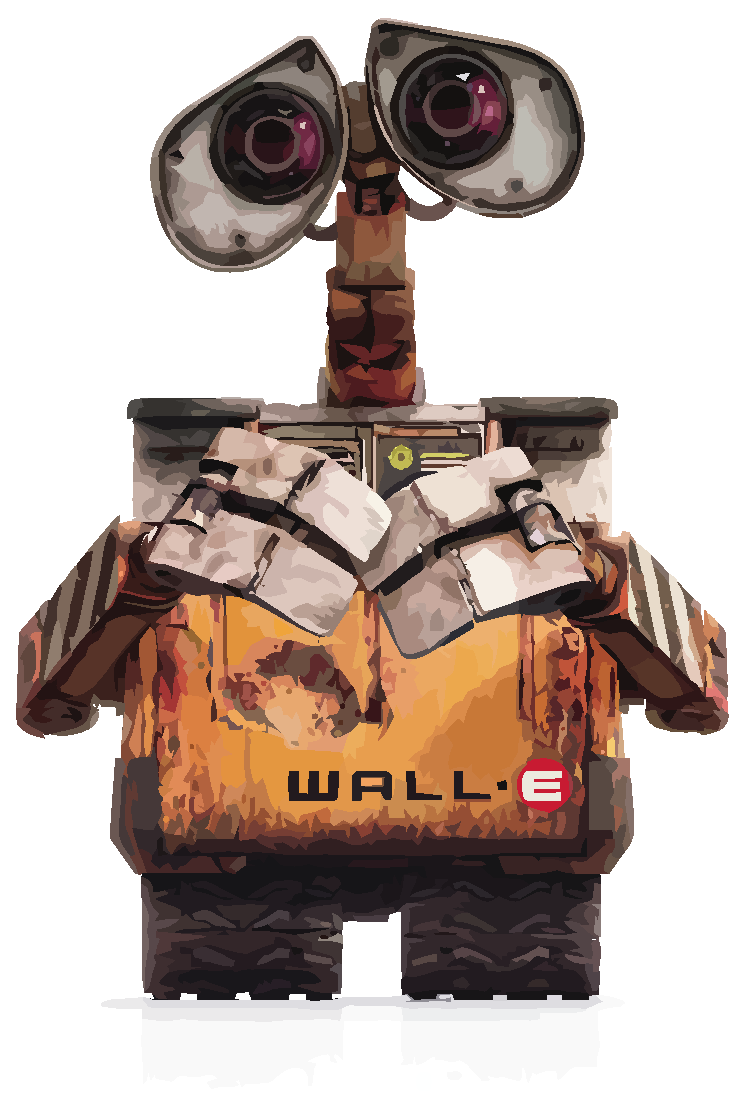
\includegraphics[width=\textwidth]{WallE}
    \caption{Wall-E}
    \label{fig:WallE}
  \end{subfigure}             
  \begin{subfigure}[b]{0.3\textwidth}
    
\includegraphics[width=\textwidth]{minion}
    \caption{Minions}
    \label{fig:Minnion}
  \end{subfigure}
  \caption{Best Animations}
  \label{fig:animations}
\end{figure}


\end{landscape}

%!TEX root = ../thesis.tex
%*******************************************************************************
%****************************** Second Chapter *********************************
%*******************************************************************************

\chapter{Generative Modelling with Latent Variable Models}

\ifpdf
    \graphicspath{{Chapter2/Figs/Raster/}{Chapter2/Figs/PDF/}{Chapter2/Figs/}}
\else
    \graphicspath{{Chapter2/Figs/Vector/}{Chapter2/Figs/}}
\fi

\emph{This chapter introduces key ideas in the literature of generative modelling with latent variable models relevant to this thesis:}
\emph{Chapter \ref{chapter:latent-space-learning-theory} presents learning theoretic results for divergence estimation in the latent spaces of autoencoders, a type of latent variable generative model;}
\emph{Chapter \ref{chapter:ica}, which concerns Independent Component Analysis (ICA), presents identifiability results for a particular class of latent variable models.}


\section{Introduction}\label{sec:generative-modelling-tour}

Suppose that a dataset of samples, drawn \iid~from some unknown data distribution $Q_X$, is given.
The high level goal of generative modelling is to learn a model distribution $P_X$ that approximates the unknown data distribution $Q_X$ based on these samples.
Latent variable models are a flexible way to specify such distributions, and work by composing simple distributions over (unobserved) latent variables with mappings to the observed data space.
The applications of latent variable generative modelling are diverse, since
having such a model of the data may be desirable for a variety of reasons, for instance: to artificially generate new samples of data \citep{goodfellow2014generative, oord2016wavenet}; to perform compression \citep{townsend2019practical, townsend2019hilloc}; to unsupervisedly learn features for transfer to other tasks \citep{tschannen2018recent, donahue2019large}; or to extract latent structure present in the data \citep{hyvarinen2000independent}.

The goal of this chapter is to introduce the necessary background and context for Chapters \ref{chapter:latent-space-learning-theory} and \ref{chapter:ica} of this thesis.
Although both concern latent variable generative models, these chapters are set in different niches of the machine learning literature.
Chapter \ref{chapter:latent-space-learning-theory} presents learning theoretic results that are relevant to the \emph{neural sampler community}, a field centred around the generation of artificial data, for which Sections \ref{sec:literature-lvms}, \ref{subsec:gen-model-divergence} and \ref{sec:literature-gen-models} of this chapter are relevant.
Chapter \ref{chapter:ica} concerns the \emph{Independent Component Analysis (ICA) community}, in which the goal is inference of latent structure, for which Sections \ref{sec:literature-lvms} and \ref{sec:literature-density-ratio-estimation} of this chapter are relevant.


%Both Chapters \ref{chapter:latent-space-learning-theory} and \ref{chapter:ica} of this thesis directly concern generative models, and the goal of this chapter is to introduce the required background.


%Generative modelling has in recent years become synonymous with the artificial generation of natural images or audio \citep{goodfellow2014generative, oord2016wavenet}.
%The mathematical formulation of this problem is, however, more general, and has close connections to other fields such as Independent Component Analysis (ICA) that will be covered in Chapter \ref{chapter:ica}.

%These correspond to (i) the community surrounding Generative Adversarial Networks (GANs) and Variational Autoencoders (VAEs), mostly relevant to Chapter \ref{chapter:latent-space-learning-theory}, will be referred to as the \emph{neural sampler community} as the goal is often to produce good quality artificial samples of data; and (ii)
%the \emph{Independent Component Analysis (ICA) community}, mostly relevant to Chapter \ref{chapter:ica}, in which the goal is inference of latent structure.



% from which new samples can be drawn. 
In the neural sampler community, the problem of generative modelling is made precise with specification of a choice of divergence
%\footnote{Defined in Section \ref{subsec:gen-model-divergence}} 
$D$ and family of distributions $P_X^\theta$ with parameter $\theta\in\Theta$, the goal then being:
%
\begin{align*}
\min_{\theta \in \Theta} \ D\left(P_X^\theta,  Q_X \right)
\end{align*}
%
There are two main challenges in practically implementing and solving this problem.
First, when the data are drawn from complex high dimensional distributions, how can this be modelled with a parameterised distribution that is computationally tractable?
Second, what are appropriate choices of divergences, and how can they be estimated or minimised with respect to the parameters $\theta$?
%These questions will be discussed in the rest of this chapter. 

In the ICA community, the goal is the use the learned model $P_X^\theta$ to infer the values of latent variables. 
Since latent variables are by definition unknown, it is important that if multiple solutions to the generative modelling problem exist, they should correspond to similar models with regard to the use of the latent variables.
That is, if distinct parameters $\theta_1 \not= \theta_2$ are such that  $P_X^{\theta_1} = P_X^{\theta_2} = Q_X$, the corresponding models should be strongly related; for instance, corresponding to the same model but with permuted coordinates over the latent variables.
Such results are known as \emph{identifiability results} and are important in the theoretical study of ICA algorithms. 
ICA will be discussed in more detail in Chapter \ref{chapter:ica}, in which novel identifiability results are presented.

%One of the main families of methods for solving this problem, autoencoders, involve the introduction of a latent space and encoder, a mapping from the data to the latent space.
%The main contribution of Chapter \ref{chapter:latent-space-learning-theory} is a learning theoretic analysis of the estimation of divergences in this latent space. 


\section{Latent variable models}\label{sec:literature-lvms}

A Latent Variable Model (LVM) is a way to specify complex distributions over potentially high-dimensional spaces using simple components. 
These are flexible models that are used widely in the machine learning literature and as such, different parts of the literature often use different terminology to describe fundamentally similar ideas.
In the following, two sets of nomenclature will be introduced for the neural sampler and ICA communities.

\medskip

\begin{definition}[Latent Variable Model]
A Latent Variable Model (LVM) over a data space $\mathcal{X}$ consists of a distribution $P_Z$ over a low dimensional latent space $\mathcal{Z}$ together with conditional distributions $P_{X|Z}$. 
Together, these induce a distribution $P_X$ over the data space. 
\end{definition}

%In practice, an LVM may be parametrised, either by parametrising the prior as $P_Z^\theta$, or the conditional distributions as $P_{X|Z}^\theta$, or both.


In the neural sampler community, $P_Z$ is referred to as a \emph{prior} or \emph{noise distribution} and is usually fixed to be some simple distribution such as a unit Gaussian or uniform distribution. 
In the ICA community, $P_Z$ is referred to as a \emph{source distribution} and may be specified only implicitly through some assumed properties, such as being a factorised distribution.

The conditional distributions can be thought of as a mapping $g:\mathcal{Z}\to\mathcal{P}(\mathcal{X})$ from elements of $\mathcal{Z}$ to distributions over $\mathcal{X}$,
and may in general be Dirac delta distributions (where all probability mass is placed at a single point), in which case the associated mapping $g$ is well-defined as a function $g:\mathcal{Z}\to\mathcal{X}$. 

In the neural sampler community, the conditional distributions are referred to as \emph{generators} or \emph{decoders}, and when given parameter $\theta$ may be written as $P_{X|Z}^\theta$ or $g^\theta$. 
If the conditional distributions they correspond to are Dirac delta distributions, the generators are called \emph{deterministic}, otherwise they are \emph{stochastic}.
In the ICA community, the generators are generally deterministic and are known as \emph{mixing functions}, and are usually denoted by $f$.

When practically implemented in modern applications, generators are often realised as neural networks.
This is straightforward in the deterministic case: $g^\theta$ is simply a function and can thus be represented as a deep network with parameters $\theta$.
If the generator is stochastic, it can still be explicitly represented as a neural network provided that the conditional distributions are sufficiently structured. 
For instance, if the conditional distributions are Gaussian with varying mean and covariance, $g^\theta$ can be represented as a neural network with two outputs, one for the mean and one for the covariance.


For a fixed choice of parameter $\theta$, $P_Z$ and $P^\theta_{X|Z}$ specify a joint distribution $P^\theta_{XZ}$ over $\mathcal{X} \times \mathcal{Z}$ and thus a distribution distribution $P_X^\theta$ over the data space $\mathcal{X}$. 
For simplicity, it will be assumed that densities of all relevant distributions exist, so that this is equivalent to specifying $P_X^\theta$ via the integral
%
\begin{align*}
p^\theta(x) = \int p^\theta(x|z) p(z) dz.
\end{align*}
%
In some special cases, the density $p^\theta(x)$ may be tractable: for instance, if the generators are deterministic and invertible with known Jacobian, as is often the case in the ICA community.
In most cases in the neural sampler community, the integral is intractable, meaning that $P_X^\theta$ has unknown density in practice.
LVMs are nonetheless useful here because samples from $P_X^\theta$ can be drawn easily:
one samples first a value $z\sim P_Z$ and then $x \sim P^\theta_{X|Z=z}$. 
All relevant distributions can be chosen so that these sampling procedures are simple, e.g.\:if $P_Z$ and all $P^\theta_{X|Z}$ are Gaussian. 


\section{Divergences}\label{subsec:gen-model-divergence}

A divergence is a notion of dissimilarity between pairs of distributions that is weaker than a metric.

\medskip

\begin{definition}
A divergence $D$ is a mapping $D: \mathcal{P}(\mathcal{X}) \times \mathcal{P}(\mathcal{X}) \to \mathbb{R} \cup \{\infty\}$ such that

\begin{itemize}
\item $D(P, Q)  \geq 0$ for any distributions $P, Q \in \mathcal{P}(\mathcal{X})$,
\item $D(P, Q) = 0$ if and only if $P = Q$,
\end{itemize}

where $\mathcal{P}(\mathcal{X})$ denotes the set of all distributions on $\mathcal{X}$.
\end{definition}


A metric is additionally symmetric and obeys the triangle inequality.
For a divergence $D(P^\theta_X, Q_X)$ to be useful in the context of generative modelling, it must be possible to minimize it with respect to the parameters $\theta$. 
There are two main families of divergences that are used in the machine learning literature generally.
At a high level, Integral Probability Metrics (IPMs) can be thought of as comparing distributions by considering the difference between their densities, while $f$-divergences can be thought of as considering the ratio of their densities.
These two families are discussed in the rest of this section.

\subsection{Integral Probability Metrics}\label{subsec:intro-ipm}

\begin{definition}
An Integral Probability Metric (IPM) is a divergence that can be written as
%
\begin{align*}
D_{\mathcal{H}}(P, Q) = \sup_{h\in\mathcal{H}} \left| \int h(x) dP(x) - \int h(x) dQ(x) \right|
\end{align*}
%
for some restricted function class $\mathcal{H}: \mathcal{X} \to \mathbb{R}$. 
\end{definition}

Elements of $\mathcal{H}$ are referred to as \emph{witness functions}.
If $\mathcal{H}$ is too small, $D_\mathcal{H}$ may not be a divergence.
For instance, taking $\mathcal{H}$ to contain only the constant $0$ function results in $D_{\mathcal{H}}(P, Q) = 0$ for any $P$ and $Q$.
On the other hand, if $\mathcal{H}$ is too rich then $D_{\mathcal{H}}$ may not be useful: 
taking $\mathcal{H}$ to be the set of all real-valued measurable functions leads to the trivial (Theorem 1, \cite{sriperumbudur2009integral})
\begin{align*}
D_{\mathcal{H}}(P, Q) = \begin{cases} 0 &\text{ if } P = Q, \\ \infty &\text{ if } P \not= Q .\end{cases}
\end{align*}
%
%which would in practice not be useful since a degree of smoothness in $P$ and $Q$ is normally desirable.
Provided $\mathcal{H}$ is sufficiently rich that $D_{\mathcal{H}}$ is a divergence, it is in fact a metric, obeying the triangle inequality and symmetry.
These properties are inherited from the function $d(x,y) = |x - y|$.
%For symmetry, observe that for any $h$, 
%%
%\begin{align*}
%\left| \int h(x) dP(x) - \int h(x) dQ(x) \right| = \left| \int h(x) dQ(x) - \int h(x) dP(x) \right|,
%\end{align*}
%%
%and thus taking the supremum over $h \in \mathcal{H}$ yields $D_{\mathcal{H}}(P, Q) = D_{\mathcal{H}}(Q, P)$. 
%For the triangle inequality


Commonly encountered IPMs include \citep{sriperumbudur2009integral}:
\begin{itemize}	
\item Wasserstein or optimal transport distances, where $\mathcal{H}$ is the set of all functions with Lipschitz constant $1$ with respect to some base metric;
\item The Total Variation distance, where $\mathcal{H}$ is the set of all functions with infinity norm $1$; and
\item The Maximum Mean Discrepancy, where $\mathcal{H}$ is the set of functions in a reproducing kernel Hilbert space with norm at most $1$ induced by some kernel $k$ \citep{gretton2012kernel}.
\end{itemize}
 
%Optimal transport distances will be discussed further in Section, making use of a different formulation of these distances than as IPMs.

\subsection{$f$-divergences}\label{subsec:f-divergences-intro}

%\begin{definition}[$f$-divergence]
%\label{def:fdiv}
%Let $f$ be a convex function on $(0, \infty)$ with $f(1) = 0$. 
%The $f$-divergence $D_f$ between distributions $Q_Z$ and $P_Z$ admitting densities $q(z)$ and $p(z)$ respectively is
%{\addtolength{\abovedisplayskip}{-0.5mm}
%\addtolength{\belowdisplayskip}{-0.5mm}
%\begin{align*}
%    D_f(Q_Z \| P_Z) := \int f \left( \frac{q(z)}{p(z)} \right) p(z) dz.
%\end{align*}}%
%\end{definition}
%Many commonly used divergences such as Kullback–Leibler and $\chi^2$ are $f$-divergences.
%All the divergences considered in this paper together with their corresponding $f$ can be found in Appendix~\ref{appendix:f-fns}. 
%Of them, possibly the least well-known in the machine learning literature are $f_\beta$-divergences \cite{osterreicher2003new}. 
%These symmetric divergences are continuously parameterized by $\beta\in(0, \infty]$. Special cases include squared-Hellinger ($\mathrm{H}^2$) for ${\beta=\frac{1}{2}}$,  Jensen-Shannon (JS) for $\beta=1$, Total Variation (TV) for $\beta=\infty$. 

%\todo{flesh out this section, give more properties of $f$-divergences?}

$f$-divergences are a family of divergences that compare pairs of distributions via their density ratio, and are widespread and important in the statistics literature \citep{csiszar2004information, liese2006divergences, tsybakov2009}

\medskip

\begin{definition}
Let $f$ be a convex real-valued function defined on $(0, \infty)$ such that $f(1)=0$, and let $P$ and $Q$ be distributions with densities $p(x)$ and $q(x)$.
The $f$-divergence between $P$ and $Q$ is defined as
%
\begin{align*}
D_f(P, Q) = \int f\left(\frac{p(x)}{q(x)}\right) q(x) dx.
\end{align*}
%
\end{definition}
This is defined for distributions $P$ and $Q$ for which $P$ is absolutely continuous with respect to $Q$, meaning informally that the density ratio $p(x)/q(x)$ is finite for all $x$ with mass under $Q$, and is usually taken to be $\infty$ otherwise.

A useful property of $f$-divergences is that for any constant $c$, replacing $f(u)$ by $\tilde{f}(u) = f(u) + c(u-1)$ does not change the divergence $D_f$:
%
\begin{align*}
D_{\tilde{f}}(P, Q) &= \int \left[ f\left(\frac{p(x)}{q(x)}\right) + c\left(\frac{p(x)}{q(x)} - 1\right) \right] q(x) dx \\
&=  \int f\left(\frac{p(x)}{q(x)}\right) q(x) dx + c \int p(x) - q(x) dx \\
&= D_f(P, Q)
\end{align*}
%
where the last equality holds since $p(x)$ and $q(x)$ integrate to $1$.
It is often convenient to work with $f_0(u) := f(u) - f'(1)(u-1)$ which is decreasing on $(0, 1)$, increasing on $(1, \infty)$ and satisfies $f'_0(1)=0$.


To see that $f$-divergences are indeed divergences, consider first non-negativity, which follows from convexity of $f$ and Jensen's inequality:
%
\begin{align}
D_f(P, Q) &= \int f\left(\frac{p(x)}{q(x)}\right) q(x) dx \nonumber \\ 
&\geq f\left(\int \frac{p(x)}{q(x)} q(x) dx\right) \label{eqn:f-divergece-jensen}\\
&= f(1) = 0. \nonumber
\end{align}
%

To show that $D_f(P,Q) = 0$ if and only if $P=Q$, note first that if $P=Q$ then $D_f(P,Q) = 0$, since $f(1)=0$.
To see that $D_f(P,Q) > 0$ for any $P \not= Q$, observe that Inequality \ref{eqn:f-divergece-jensen} above is strict for any $f$ that is strictly convex.
%
This also holds for any $f$ that does not have constant gradient in any neighbourhood of $1$, since the $f_0$ associated to any such $f$ is strictly positive on $\mathbb{R}_+\setminus \{1\}$.
For any $P\not= Q$, the distribution $Q$ must put positive mass in areas for which $p(x)/q(x) \not= 1$ and so  $D_{f_0}(P,Q)$ must be positive.
It follows that $D_f = D_{f_0}$ is also positive.
Hence `most' choices of $f$ lead to valid $f$-divergences.


Different choices of $f$ yield several commonly encountered divergences, including the Kullback-Leibler, Jensen-Shannon, Total Variation, $\chi^2$ and $\alpha$-divergences as well as the lesser known $\beta$-divergences \citep{osterreicher2003new}.
This family of symmetric divergences are continuously parameterized by $\beta\in(0, \infty]$ and include as special cases the squared-Hellinger $({\beta=\frac{1}{2}})$,  Jensen-Shannon $(\beta=1)$ and Total Variation $(\beta=\infty)$. 
Table \ref{table:f-fns} lists the corresponding $f_0$ for the divergences considered in Chapter \ref{chapter:latent-space-learning-theory}.

%This is similarly the case for any $f$ for which there exists some $c>0$ such that $f(u) > c(u-1)$ for all $u\not=1$. 
%
%Indeed, for any $P \not= Q$ there exists a set $A \subset \mathcal{X}$ with positive measure under $Q$ on which $p(x)/q(x) \not= 1$ (if this were not the case, we would have $p(x)/q(x) = 1$ everywhere that $Q$ puts mass and so $P=Q$).
%Thus,
%\begin{align*}
%D_f(P, Q) &= \int_A f\left(\frac{p(x)}{q(x)}\right) q(x) dx +  \int_{\mathcal{X} \setminus A} f\left(\frac{p(x)}{q(x)}\right) q(x) dx\\ 
%&> \int_A c \left(\frac{p(x)}{q(x)} - 1\right) q(x) dx +  \int_{\mathcal{X} \setminus A} c \left(\frac{p(x)}{q(x)} - 1\right) q(x) dx\\ 
%&= c > 0.
%\end{align*}





%\section{$f$ for divergences considered in this paper}\label{appendix:f-fns}



{
\renewcommand{\arraystretch}{2}
\begin{table}
 \caption{$f_0$ corresponding to divergences referenced in this thesis.}
 \label{table:f-fns}
 \centering
 \begin{tabular}{c c} 
 \toprule
 $f$-divergence & $f_0(x)$ \\
 \midrule
 Kullback-Leibler (KL) & $x \log x - x + 1$\\
 Total Variation (TV) & $\frac{1}{2}|1-x|$\\
 $\chi^2$ & $x^2 - 2x$\\
 Squared-Hellinger ($\text{H}^2$) & $2(1-\sqrt{x})$\\
 Jensen-Shannon (JS) & $(1+x)\log(\frac{2}{1+x}) + x\log x$\\
 $\alpha$-divergence, \,
% $D_{f_\alpha}$, 
 $-1<\alpha < 1$ & $\frac{4}{1-\alpha^2}\left( 1 - x^{\frac{1+\alpha}{2}} \right) - \frac{2(x-1)}{\alpha-1}$ \\
 $\beta$-divergence, \,
% $D_{f_\beta}$, 
 $\beta > 0,$ $\beta\not=\frac{1}{2}$ & $\frac{1}{1-\frac{1}{\beta}}\left[ (1+x^\beta)^{\frac{1}{\beta}} - 2^{\frac{1}{\beta}-1}(1+x) \right]$\\
 \bottomrule
\end{tabular}
\end{table}
}


%\begin{align*}
%D_f(P, Q) = 
%    \begin{cases}
%       \int f\left(\frac{dQ}{dP}(x) \right) dP, & \text{if $dQ/dP$ exists} \\
%      \infty, & \text{otherwise}
%    \end{cases}
%\end{align*}

%Intuitively, such divergences measure the discrepancy between the two distributions by seeking functions which are maximal on one distribution and minimal on the other. 



\section{Density Ratio Estimation}\label{sec:literature-density-ratio-estimation}

A natural way to distinguish between two distributions $P$ and $Q$ with overlapping support is to consider the problem of classifying between draws from each distribution.
Suppose that samples from $P$ are labelled as class $1$, and samples from $Q$ as class $0$. 
This classification problem implemented as logistic regression, in which case a function $c:\mathcal{X}\to [0,1]$ is introduced and trained to minimise the objective 
%
\begin{align*}
L(c) &=  \mathbb{E}_{x\sim P}\left[ - \log c(x) \right] + \mathbb{E}_{x \sim Q} \left[ - \log(1 - c(x)) \right] \\
&= \int -\log c(x) p(x) - \log (1 - c(x)) q(x) dx
\end{align*}
%
For any particular $x$, the integrand is minimised by $c^*(x) = \frac{p(x)}{q(x) + p(x)}$ \citep{goodfellow2014generative}, and so the optimal classifier assigns $x$ to class $1$ with the posterior probability that it was drawn from $P$.
If $c$ parametrised as $\frac{1}{1+\exp( -r(x))}$ where $r:\mathcal{X}\to\mathbb{R}$, then the optimal  $c^*$ corresponds to $r^*(x) = \log\left(p(x) / q(x)\right)$.

This is a useful trick for cases in which only samples from two distributions are available and estimation of their density ratio is desired, as is the case in Chapter \ref{chapter:ica}.
Moreover, solving this classification problem is closely related to divergence estimation, since for any choice of classifier $c$,
%
\begin{align*}
L(c) \geq \log 4 - 2 \cdot D_{\text{JS}}(P, Q).
\end{align*}
%
This follows straightforwardly from the definition of the Jensen-Shannon divergence and the fact that equality is attained by the optimal $c^*$, see \cite{goodfellow2014generative} for details.
Rearranging, it follows that the Jensen-Shannon divergence between two distributions can be estimated by maximising the lower bound
%
\begin{align*}
D_{\text{JS}}(P, Q) \geq \log 2 - \frac{L(c)}{2}.
\end{align*}

Recall that the Jensen-Shannon divergence is an $f$-divergence. 
It can be similarly shown that any $f$-divergence between two distributions can be estimated by maximisation of a lower bound corresponding to a classification problem, and that doing so results in a function of the density ratio being estimated.
All $f$-divergences admit a variational form as a result of convex conjugacy \citep{nguyen10ratio}.
Any convex function $f(u)$ has a conjugate $f^*(t)$ defined as
%
\begin{align*}
f^*(t) = \sup_{u \in \dom(f)} \{ut - f(u)\}.
\end{align*}
%
The resulting function $f^*$ is itself convex, and
provided that $f$ is continuous, $f$ and $f^*$ are dual in the sense that $f^{**} = f$.
This means that $f$ can be written as
%
\begin{align*}
f(u) = \sup_{t \in \dom(f^*)} \{ut - f^*(t)\}.
\end{align*}
%
Plugging this into the definition of $f$-divergences yields
%
\begin{align*}
D_f(P, Q) &= \int q(x) \sup_{t \in \dom(f^*)} \left\{t \frac{p(x)}{q(x)} - f^*(t) \right\} dx \\
& \geq \sup_{T \in \mathcal{T}} \left\{ \int p(x) T(x) dx - \int q(x) f^*(T(x)) \right\} dx \\
&= \sup_{T \in \mathcal{T}} \mathbb{E}_{x \sim P} \left[ T(x) \right] - \mathbb{E}_{x \sim Q} \left[ f^*(T(x)) \right] 
\end{align*}
where $\mathcal{T}$ is an arbitrary class of functions $\mathcal{X} \to \dom(f^*) \subseteq \mathbb{R}$.
It can be shown \citep{nguyen10ratio} that the optimal $T^*$ attaining the supremum satisfies 
\begin{align*}
T^*(x) = f'\left( \frac{p(x)}{q(x)}\right)
\end{align*}
subject to mild conditions on $f$. 
In this sense, $T^*$ estimates (a function of) the density ratio $p(x)/q(x)$.

%The particular case of the Jensen-Shannon divergence merits further discussion for two reasons.
%First, it is relevant to the explanation of Generative Adversarial Networks in the next section. 
%Second, because it is used in Chapter \ref{chapter:ica}.




%In this chapter we do not make use of this variational formulation of $f$-divergences, but it will be used in explaining Generative Adversarial Networks in the next section.


\section{Examples of generative models}\label{sec:literature-gen-models}

Solving the generative modelling problem as posed in the introduction requires the minimisation of $D(P^\theta_X, Q_X)$ with respect to the parameters $\theta$ of the LVM in a computationally tractable way.
In general it is infeasible to estimate $D(P^\theta_X, Q_X)$ directly, or even to compute gradients of it with respect to $\theta$. 
%Thus, one must resort to approximations.


There are two main families of methods that introduce auxiliary functions as computational tricks to bound or estimate $D(P^\theta_X, Q_X)$ in a computationally tractable way.
These are \emph{Generative Adversarial Networks (GANs)}, which introduce a discriminator $d:\mathcal{X} \to [0,1]$, and \emph{autoencoders}, which introduce an encoder $e:\mathcal{X} \to \mathcal{Z}$.

The remainder of this section discusses GANs and two types of autoencoders, Variational Autoencoders (VAEs) and Wasserstein Autoencoders (WAEs), showing how specific choices of divergences can be approximated.

\subsection{Generative Adversarial Networks}

Generative Adversarial Networks (GANs) are a family of methods that approximately minimise any $f$-divergence and some choices of IPMs. 
In the case of $f$-divergences, the key ideas have been already introduced in Section \ref{sec:literature-density-ratio-estimation}.

\cite{goodfellow2014generative} introduced the idea of training a discriminator $d^\phi: \mathcal{X} \to [0,1]$ to classify between `real' samples from $Q_X$ and `fake' samples from $P^\theta_X$, which then provides a surrogate loss for a generator $g^\theta$, trained simultaneously to maximise the loss of the discriminator. 
In \cite{goodfellow2014generative}, the loss is implemented as logistic regression
%
\begin{align*}
L(\theta, \phi) = \mathbb{E}_{x\sim Q_X}\left[ -\log d^\phi(x) \right] \mathbb{E}_{x \sim P_Z} \left[- \log(1 - d^\phi(g^\theta(z)) \right]
\end{align*}
%
which, as previously discussed in Section \ref{sec:literature-density-ratio-estimation}, is a lower bound on the Jensen-Shannon divergence $D_{\text{JS}}(P^\theta_X, Q_X)$, up to constants and scalar factors.

Stochastic gradients of this loss can be taken with respect to both $\phi$ and $\theta$ by using minibatch samples of data to approximate the outer expectations when $d^\phi$ and $g^\theta$ are both neural networks.
%It was shown that this loss satisfies $L(\theta, \phi) \leq 2 \cdot D_{\text{JS}}(P^\theta_X, Q_X) - \log 4$ for any $d^\phi$ and $g^\theta$, with equality attainable only if the class of $d^\phi$ is sufficiently rich, where $D_{\text{JS}}$ is the Jensen-Shannon divergence.
Thus, although actually computing $D_{\text{JS}}(P^\theta_X, Q_X)$ is intractable, it can be approximately minimised with respect to $\theta$ by maximising the surrogate loss $L(\theta, \phi)$ with respect to $\phi$ and minimising it with respect to $\theta$.
%is (up to constants) a lower bound on this.
%Hence the Jensen-Shannon divergence can be approximately minimised by \emph{maximising} $L(\theta, \phi)$ with respect to $\phi$ and minimising this with respect to $\theta$.


\cite{nowozin2016f}, building on the work of \cite{nguyen10ratio}, generalised this to arbitrary $f$-divergences using the variational formulation of $f$-divergences to yield the surrogate loss
%
%\begin{align*}
%D_f(P, Q) &\geq \sup_{T \in \mathcal{T}} \mathbb{E}_{x \sim P} \left[ T(x) \right] - \mathbb{E}_{x \sim Q} \left[ f^*(T(x)) \right] 
%\end{align*}
%%
%where the set of functions $\mathcal{T}$ is implemented as a neural network.
%Thus, parameterising $T$ by $\phi$ yields the surrogate loss
%
\begin{align*}
L_f(\phi, \theta) = \mathbb{E}_{x \sim Q_X} \left[ T^\phi(x) \right] - \mathbb{E}_{z \sim P_Z} \left[ f^*(T^\phi(g^\theta(x))) \right] \leq D_f(P^\theta_X, Q_X)
\end{align*}
%
where the function $T^\phi$ is implemented as a neural network.
As with the original GAN objective, stochastic gradients of this surrogate loss can be computed. 
The function $T^\phi$ plays the role of the discriminator introduced by \cite{goodfellow2014generative}. %but the above derivation holds for arbitrary choices of $f$. 
\cite{nowozin2016f} thus demonstrated how the GAN `trick' can be applied to other $f$-divergences to approximately minimise $D_f(P^\theta_X, Q_X)$ with respect to the LVM parameters $\theta$.

A similar idea can also be used to approximately minimise IPMs $D_\mathcal{H}(P^\theta_X, Q_X)$, provided that the function class $\mathcal{H}$ can be practically parameterised.
If $\mathcal{H}$ is such that $h \in \mathcal{H}$ implies that $-h \in \mathcal{H}$, $D_\mathcal{H}$ can be written without the inner absolute function, leading to
%
\begin{align*}
D_{\mathcal{H}}(P, Q) &= \sup_{h\in\mathcal{H}} \int h(x) dP(x) - \int h(x) dQ(x) \\
&= \sup_{h\in\mathcal{H}} \left\{ \mathbb{E}_{x \sim P} \left[ h(x) \right]- \mathbb{E}_{x \sim Q} \left[ h(x) \right] \right\} \\
&\geq  \mathbb{E}_{x \sim P} \left[ h(x) \right]- \mathbb{E}_{x \sim Q} \left[ h(x) \right] \\
\end{align*}
%
where the inequality holds for any $h \in \mathcal{H}$, where $h$ now plays the role of the discriminator. 
If the elements of $\mathcal{H}$ can be differentiably parametrised, stochastic gradients of the loss can be obtained with respect its parameters.
In contrast to the $f$-divergence case, the discriminator $h$ must belong to a particular class of functions, which can complicate specifying the parametrisation.
One example of an IPM-based GAN is the Wasserstein GAN of \cite{AB17}. 
Here, the 1-Wasserstein distance is used, corresponding to $h$ having Lipschitz constant at most $1$. 
For certain neural network architectures, including those composed of fully-connected and convolutional layers, this can be enforced by weight clipping.

\subsection{Variational Autoencoders}

Variational Autoencdoers (VAEs) \citep{kingma2013auto, rezende2014stochastic} are a method to minimize the KL-divergence between model and data distributions, defined as
%
\begin{align*}
D_{\text{KL}}(Q_X, P^\theta_X) &= \int q(x) \log \left( \frac{q(x)}{p^\theta(x)} \right) dx \\
&= \int q(x) \log q(x) - \int q(x) \log p^\theta(x) dx.
\end{align*}
%
The first term above, the negative of the \emph{differential entropy} of $Q_X$, often written $H(Q_X)$, cannot be estimated without knowledge of the density $q(x)$.
However, since it is constant as a function of $\theta$, it can be ignored.
The term $\log p^\theta(x)$ inside the second integral is known as the \emph{log-likelihood} or \emph{evidence}, and maximisation of this quantity is known as \emph{maximum likelihood estimation}. 
Although the density $p^\theta(x)$ is intractable, the evidence can be tractably lower bounded leading to the so-called \emph{evidence lower bound} (ELBO), which in turn leads to a tractable \emph{upper} bound on $D_{\text{KL}}(Q_X, P^\theta_X)$. 

First, observe that the log-likelihood can be written 
%
\begin{align*}
\log p^\theta(x) &= \log \left( \int p^\theta(x|z) p(z) dz \right).
\end{align*}
%
Given any distribution $q^\phi(z|x)$ depending on parameter $\phi$ and the value of $x$, we can multiply and divide inside the integral, leaving its value unchanged.
This leads to
%
\begin{align*}
\log p^\theta(x) &= \log \left( \int p^\theta(x|z) \frac{p(z)}{q^\phi(z|x)} q^\phi(z|x) dz \right) \\
&= \log \left( \mathbb{E}_{q^\phi(z|x)} \left[  p^\theta(x|z) \frac{p(z)}{q^\phi(z|x)} \right]\right) \\
&\geq \mathbb{E}_{q^\phi(z|x)} \left[ \log p^\theta(x|z) + \log p(z) - \log q^\phi(z|x) \right] \\
&= \mathbb{E}_{q^\phi(z|x)} \log p^\theta(x|z)  - D_{\text{KL}}\left(q^\phi(z|x), p(z)\right),
\end{align*}
%
where the inequality follows from Jensen's inequality due to the concavity of $\log$.
The distribution $q^\phi(z|x)$ is a variational approximation to the true posterior $p^\theta(z|x)$; it can be shown that the gap introduced by Jensen's inequality is equal to $D_{\text{KL}}\left(q^\phi(z|x), p^\theta(z|x)\right)$. 
$q^\phi(z|x)$ is often referred to as an encoder as it maps elements of the data space $\mathcal{X}$ to distributions over the latent space $\mathcal{Z}$.
Putting things together yields
%
\begin{align*}
D_{\text{KL}}(Q_X, P^\theta_X) \leq -H(Q_X)  - \mathbb{E}_{q(x)} \mathbb{E}_{q^\phi(z|x)} \log p^\theta(x|z) + \mathbb{E}_{q(x)}D_{\text{KL}}\left(q^\phi(z|x), p(z)\right)
\end{align*}
%
where $H(Q_X)$ is the constant differential entropy, leading to the VAE loss
%
\begin{align}
L_{\text{VAE}}(\theta, \phi) =  \underbrace{\mathbb{E}_{q(x)} \mathbb{E}_{q^\phi(z|x)} \left[ - \log p^\theta(x|z)\right]}_{\text{(i)}} + \underbrace{\mathbb{E}_{q(x)}D_{\text{KL}}\left(q^\phi(z|x), p(z)\right)}_{\text{(ii)}}
\end{align}
%
which (up to constants) is an upper bound on $D_{\text{KL}}(Q_X, P^\theta_X)$.
It is common for the prior to be a standard Gaussian, the generator to output Gaussians with mean $\mu^\theta(z)$ and fixed isotropic covariance, and the encoder to map to Gaussians with mean $\mu^\phi(x)$ and diagonal covariance $\Sigma^\phi(x)$.
In this case, term (i) above can be interpreted as an average reconstruction loss and (ii) as a regulariser, hence making the model a type of regularised autoencoder\footnote{Note however that the interpretation of VAEs as a type of autoencoder breaks down when more powerful classes of generators are used, as discussed in \href{http://paulrubenstein.co.uk/variational-autoencoders-are-not-autoencoders/}{http://paulrubenstein.co.uk/variational-autoencoders-are-not-autoencoders/}.}.

The encoder $Q^\phi_{Z|X}$ together with the data distribution $Q_X$ induce the push-forward distribution $Q^\phi_Z$ known as the \emph{aggregate posterior}.
The term (ii) was shown by \cite{hoffman2016elbo} to be equivalent to $D_{\text{KL}}(Q^\phi_Z , P_Z) + I(X,Z)$ where $I(X,Z) = D_{\text{KL}}(Q^\phi_{XZ} , Q_XQ^\phi_{Z})$ is the mutual information of a data sample and its encoding.
Chapter \ref{chapter:latent-space-learning-theory} concerns estimation of $f$-divergences (and hence the KL-divergence) between priors and aggregate posteriors, and so is directly relevant mutual information estimation via this equivalence.

%All distributions involved can be chosen so this can be unbiasedly estimated, meaning that it can be minimised with respect to the parameters $\theta$ and $\phi$ using stochastic gradient methods.
%It is common that the encoder, generator and prior are chosen to be Gaussians, 



%\todo{discuss the fact that the aggregate posterior and prior satisfy the setting we consider and mention that some works consider divergences between them?}

\subsection{Wasserstein Autoencoders}

Wasserstein Autoencoders (WAEs) \citep{tolstikhin2017wasserstein} approximately minimise optimal transport distances, also known as 1-Wasserstein distances, between model and data distributions.
These were discussed briefly in Section \ref{subsec:intro-ipm} as they can be expressed as IPMs, but here an alternative formulation of these distances will be used.

Let $c$ be any metric on $\mathcal{X}$.
For intuition, $c(x, x')$ may be thought of as a function specifying the cost of transporting a point from $x$ to $x'$.
The optimal transport distance between two distributions $P$ and $Q$ over $\mathcal{X}$ is then the minimal cost incurred by transporting the probability mass of $P$ to that of $Q$.
%For simplicity in the following, we will assume $P$ and $Q$ have densities $p$ and $q$. 

Formally, let $\Gamma$ be the set of joint distributions over $\mathcal{X} \times \mathcal{X}$ with marginals $P$ and $Q$. 
That is, any element $\gamma(x, x') \in \Gamma$ is a joint distribution satisfying $\gamma(x) = p(x)$ and $\gamma(x') = q(x')$.
Then, the optimal transport distance is defined as
%
\begin{align*}
OT_c(P, Q) = \min_{\gamma \in \Gamma} \mathbb{E}_{x, x' \sim \gamma} \left[ c(x, x') \right].
\end{align*}
%
This can equivalently be written as
%
\begin{align*}
OT_c(P, Q) = \min_{\gamma \in \Gamma} \mathbb{E}_{x\sim Q} \mathbb{E}_{x'\sim \gamma(x'|x)} \left[ c(x, x') \right],
\end{align*}
%
where $\gamma$ can be though of as a conditional distribution specifying how an element of probability mass at $x$ should be moved and spread over the points $x'$. 
Specified this way, each element of $\Gamma$ should satisfy $\int \gamma(x'|x) q(x) dx = p(x')$.
In the generative modelling setting, we thus have
%
\begin{align*}
OT_c(P_X^\theta, Q_X) = \min_{\gamma \in \Gamma} \mathbb{E}_{x\sim Q_X} \mathbb{E}_{x'\sim \gamma(x'|x)} \left[ c(x, x') \right].
\end{align*}
%
In practice, this minimisation problem cannot be solved directly: given a candidate conditional distribution $\gamma(x'|x)$ it is not practically possible to verify whether or not $\int \gamma(x'|x) q_X(x) dx = p_X^\theta(x')$ since only samples from $Q_X$ are available and the density $p^\theta_X(x)$ is intractable.

\cite{tolstikhin2017wasserstein} proved the following result, giving a handle on this problem:
If the generator $p^\theta(x|z)$ is deterministic, any valid $\gamma$ can be written as a composition $\gamma(x'|x) = \int p^\theta(x'|z) q^\phi(z|x) dz$ where $q^\phi(z|x)$ is a conditional distribution satisfying $\int q^\phi(z|x) q(x) dx = p(z)$. 
That is, any $\gamma$ can be `factored through' the latent space by introducing an encoder $q^\phi(z|x)$, replacing the constraint of distribution matching in the data-space ($\int \gamma(x'|x) q_X(x) dx = p_X^\theta(x')$) with distribution matching in the latent space ($\int q^\phi(z|x) q(x) dx = p(z)$).

Intuitively, $P_Z$ is a different parametrisation of $P_X^\theta$ and so if $Q_X$ pushed through the encoder results in $P_Z$, pushing $Q_X$ through the composition of the encoder and the generator will result in $P_X^\theta$. 
While it is clear that the composition of any such encoder and the generator induces a valid $\gamma$, it is non-trivial that any $\gamma$ can be decomposed as such. 
This is proved in Theorem 1 of \cite{tolstikhin2017wasserstein}.

Writing $Q_Z = \int Q_{Z|X=x} q(x) dx$ to be the latent space distribution obtained by pushing the data through the encoder and $g$ for the deterministic generator yields the following alternative statement of the optimal transport distance in the LVM setting:
%
\begin{align*}
OT_c(P_X^\theta, Q_X) = \min_{Q_{Z|X}: Q_Z = P_Z} \mathbb{E}_{x\sim Q_X} \mathbb{E}_{z\sim Q_{Z|X=x}} \left[ c(x, G(z)) \right].
\end{align*}
%
Again this optimisation problem is not feasible to solve due to the hard constraint, 
but it can be made computationally feasible by relaxing the constraint to obtain the WAE objective:
%
\begin{align}
L_{\text{WAE}}^{\lambda, D}(\theta, \phi) = \underbrace{\mathbb{E}_{x\sim Q_X} \mathbb{E}_{z\sim Q^\phi_{Z|X=x}} \left[ c(x, G^\theta(z)) \right]}_{\text{(i)}} + \underbrace{\lambda D\left(Q^\phi_Z, P_Z  \right)}_{\text{(ii)}}
\end{align}
%
where $D$ is some divergence, $\lambda$ is a positive scalar and the encoder is given parameter $\phi$.
While the generator is required to be deterministic, the encoder may be deterministic or stochastic \citep{rubenstein2018latent}.
For general choices of $\lambda$ and $D$, $\inf_{\phi} L_{\text{WAE}}^{\lambda, D}(\theta, \phi)$ is neither an upper nor lower bound on the original objective $OT_c(P_X^\theta, Q_X)$, but a heuristic approximation due to the relaxation of the constraint. 

%It was, however, proven by \cite{sinkhorn} (Theorem 2.1) that if $G$ is $\lambda$-Lipschitz, , then taking $D$ to be

Term (i) of the WAE loss is simply a reconstruction loss, corresponding to the average distance between data sampled from $Q_X$ and their reconstruction obtained by pushing through the encoder and decoder.
This is therefore simple to estimate and optimise with respect to the parameters $\phi$ and $\theta$.
Term (ii) is potentially challenging to estimate depending on the choice of $D$. 
\cite{tolstikhin2017wasserstein} propose two choices for $D$ which can be estimated based on samples from $P_Z$ and $Q_Z^\phi$: the Maximum Mean Discrepancy (MMD) \citep{gretton2012kernel} which can be estimated directly, leading to WAE-MMD, and a GAN style estimation of the Jensen-Shannon divergence by introducing an additional discriminator to obtain a lower bound on the divergence, leading to WAE-GAN. 

Estimating a divergence between $P_Z$ and $Q_Z^\phi$ using sample-based methods does not make use of a significant degree of structure that is present in the problem. $P_Z$ is typically chosen to be a simple distribution with known density. While $Q_Z^\phi$ may be complex, its density can be decomposed as $q^\phi(z) = \mathbb{E}_{x\sim Q_X} q^\phi(z|x)$ where $q^\phi(z|x)$ is also typically chosen to be simple (e.g. Gaussian) and $Q_X$ can be sampled.
The main contribution of Chapter \ref{chapter:latent-space-learning-theory} is to propose and analyse an estimator making use of this structure for the case that $D$ in (ii) is chosen to be an $f$-divergence. 


%
%!TEX root = ../thesis.tex
%*******************************************************************************
%****************************** Third Chapter **********************************
%*******************************************************************************
\chapter{Latent Space Learning Theory}\label{chapter:latent-space-learning-theory}

% **************************** Define Graphics Path **************************
\ifpdf
    \graphicspath{{Chapter5/Figs/Raster/}{Chapter5/Figs/PDF/}{Chapter5/Figs/}}
\else
    \graphicspath{{Chapter5/Figs/Vector/}{Chapter5/Figs/}}
\fi

\emph{This chapter presents and analyses RAM-MC, an f-divergence estimator that is applicable to estimating divergences between particular distributions in the latent spaces of autoencoder models such as Variational Autoencoders and Wasserstein Autoencoders. 
Learning theoretic analyses of sampled-based $f$-divergence estimators usually yield poor rates of convergence unless strong assumptions are made.
By exploiting the natural structure present in the autoencoder setting, RAM-MC exhibits fast rates under mild assumptions.}

\emph{This work is an important contribution to the literature for two main reasons. 
First, it demonstrates that the $f$-divergences considered can be estimated with a practical number of samples.
Second, it provides a rigorous foundation to related methods that have been heuristically proposed elsewhere in the literature.}

\emph{The main technical content of this chapter has been published in the paper:}

\begin{quote}
\fullcite{rubenstein2019practical}
\end{quote}

%\emph{Additionally, the following related workshop papers were published during my PhD but are not included in this thesis:}
%
%\begin{quote}
%\fullcite{rubenstein2018wasserstein}
%\end{quote}
%
%\begin{quote}
%\fullcite{rubenstein2018learning}
%\end{quote}
%
%\emph{The main contribution of this chapter is a learning theoretic analysis of estimating divergences between distributions. 
%The setting considered by this work occurs naturally in and has application to the latent variable models used in the generative modelling community, in particular Wasserstein Autoencoders.
%Sections ?? - ?? are a review of generative modelling, setting the stage for Sections ?? - ?? which is based on} \cite{rubenstein2019practical}.
%
%\todo{replace $D(.\|.)$ with $D(.,.)$}

%\todo{Consistent use of -divergence and whether $H^2$ is italicised or not}

\section{Introduction}

The estimation and minimisation of divergences between probability distributions based on samples are fundamental problems of machine learning.
The previous chapter discussed generative modelling, but there are numerous other applications across the literature.
For example, 
%maximum likelihood learning can be viewed as minimizing the Kullback-Leibler divergence $D_{\text{KL}}(P_{\text{data}}, P_{\text{model}})$ with respect to the model parameters.
%More generally, generative modelling
%%---most famously Variational Autoencoders and Generative Adversarial Networks \cite{kingma2013auto, goodfellow2014generative} discussed in the next section---
%can be viewed as minimizing a divergence $\smash{D(P_{\text{data}}, P_{\text{model}})}$ where $\smash{P_{\text{model}}}$ may be intractable.
in variational inference, an intractable posterior $p(z|x)$ is approximated with a tractable distribution $q(z)$ chosen to minimise the Kullback-Leibler ($\KL$) divergence $\smash{D_{\text{KL}}\bigl(q(z) , p(z|x)\bigr)}$.
The mutual information between two variables $\smash{I(X,Y)}$, core to information theory and Bayesian machine learning, is equivalent to $\smash{D_{\text{KL}}(P_{X,Y} , P_X P_Y)}$. 
Independence testing often involves estimating a divergence $\smash{D(P_{X,Y} , P_X P_Y)}$, while two-sample testing (does $P=Q$?) involves estimating a divergence $D(P,Q)$.
Additionally, one approach to domain adaptation, in which a classifier is learned on a distribution $P$ but tested on a distinct distribution $Q$, involves learning a feature map $\phi$ such that a divergence $\smash{D\left( \phi_\# P , \phi_\# Q \right)}$ is minimised, where $\smash{\phi_\#}$ represents the push-forward operation \citep{ben2007analysis,ganin2016domain}.

This chapter concerns the estimation of $f$-divergences, introduced in Section \ref{subsec:f-divergences-intro}.
%This chapter considers the well-known family of $f$-divergences \cite{csiszar2004information, liese2006divergences} that includes amongst others the $\KL$, Jensen-Shannon ($\JS$), $\chi^2$, and $\alpha$-divergences as well as the Total Variation ($\TV$) and squared Hellinger ($\Hsq$) distances, the latter two of which play an important role in the statistics literature \cite{tsybakov2009}.
A significant body of work exists studying estimation of $D_f(P , Q)$ for general probability distributions $P$ and $Q$.
While the majority of this focuses on $\alpha$-divergences and closely related R\'enyi-$\alpha$ divergences \citep{poczos11alpha, singh14alpha, krishnamurthy14icml},
many works address specifically the KL-divergence \citep{perez08kl, wang09kl}
with fewer considering $f$-divergences in full generality \citep{nguyen10ratio, kanamori12ratio, moon14ensemble, moon14followup}.
Although the $\KL$-divergence is the most frequently encountered $f$-divergence in the machine learning literature, in recent years there has been growing interest in other $f$-divergences \citep{nowozin2016f,zhang2019variational}, 
in particular in the variational inference community where they have been employed to derive alternative evidence lower bounds \citep{li2016renyi, dieng2017variational, pmlr-v80-chen18k}.


The main challenge in computing $D_f(P , Q)$ is that it requires knowledge of either both densities $p(x)$ and $q(x)$, or the density ratio $p(x)/q(x)$.
In studying this problem, assumptions of differing strength can be made about $P$ and $Q$. 
In the weakest \emph{agnostic} setting, one may be given only a finite number of \iid~samples from the distributions without any further knowledge of their densities.
As an example of stronger assumptions,
both distributions may be mixtures of Gaussians \citep{hershey2007approximating, durrieu2012lower}, 
or one may have access to samples from $Q$ and have full knowledge of $P$ as in e.g.~model fitting \citep{heroma2001techrep, heroma2002ieee}.

Most of the literature on $f$-divergence estimation considers the weaker agnostic setting.
The lack of assumptions makes such work widely applicable, but comes at the cost of needing to work around estimation of either the densities $p(x)$ and $q(x)$ \citep{singh14alpha, krishnamurthy14icml} or the density ratio $p(x)/q(x)$ \citep{nguyen10ratio, kanamori12ratio} from samples.
Both of these estimation problems are provably hard \citep{tsybakov2009, nguyen10ratio} and suffer rates---the speed at which the error of an estimator decays as a function of the number of samples $N$---of order $\smash{N^{-1/d}}$ when $P$ and $Q$ are defined over $\R^d$ unless their densities are sufficiently smooth.
This is a manifestation of the \emph{curse of dimensionality} and rates of this type are often called \emph{nonparametric}.
One could hope to estimate $D_f(P,Q)$ without explicitly estimating the densities or their ratio and thus avoid suffering nonparametric rates, however a lower bound of the same order $\smash{N^{-1/d}}$ is known for $\alpha$-divergences \citep{krishnamurthy14icml}, a sub-family of $f$-divergences.
While some works considering the agnostic setting provide rates for the bias and variance of the proposed estimator \citep{nguyen10ratio, krishnamurthy14icml} or even exponential tail bounds \citep{singh14alpha},
it is more common to only show that the estimators are asymptotically unbiased or consistent without proving specific rates of convergence \citep{wang09kl, poczos11alpha, kanamori12ratio}.


Motivated by recent advances in machine learning, this chapter considers a setting in which structural assumptions are made about the distributions.
Although the assumptions are strong, they are naturally satisfied in the setting of autoencoders such as Wasserstein Autoencoders and Variational Autoencoders.


Let $\X$ and $\Z$ be two finite dimensional Euclidean spaces.
This chapter studies estimation of the divergence $D_f(Q_Z, P_Z)$ between two probability distributions $P_Z$ and $Q_Z$, both defined over $\Z$.
It is assumed that $P_Z$ has known density $p(z)$, while $Q_Z$ with density  $q(z)$ admits the factorization $\smash{q(z) = \int q(z|x)q(x) dx}$.
Access to independent samples from the distribution $Q_X$ with unknown density $q(x)$ and full knowledge of the conditional distribution $\smash{Q_{Z|X}}$ with density $q(z|x)$ are assumed.
%The true density $q(z)$ is unknown due to the integral over the unknown $q(x)$ and so is $D_f(Q_Z , P_Z)$.
In the language of autoencoders,
%As a concrete example, these assumptions are often satisfied in applications of modern unsupervised generative modeling with deep autoencoder architectures,
%where 
$\X$ and $\Z$ would be \emph{data} and \emph{latent} spaces, $\smash{P_Z}$ the \emph{prior}, $\smash{Q_X}$ the \emph{data distribution}, $\smash{Q_{Z|X}}$ the \emph{encoder}, and $\smash{Q_Z}$ the \emph{aggregate posterior}, though the theory presented in this work does not apply exclusively to this setting.

Given independent observations $\smash{X_1, \ldots, X_N}$ from $\smash{Q_X}$, the goal is to estimate $\smash{D_f(Q_Z , P_Z)}$.
The main contribution of this chapter is to use the finite mixture $\smash{\hat{Q}_Z^N := \frac{1}{N} \sum_{i=1}^N Q_{Z|X_i}}$ as a surrogate for the continuous mixture $\smash{Q_Z}$, 
to use this to approximate $\smash{D_f(Q_Z , P_Z)}$ with $\smash{D_f(\hat{Q}_Z^N , P_Z)}$,
%a quantity that can be estimated to arbitrary precision using Monte-Carlo sampling since both distributions have known densities, 
and to theoretically study conditions under which this approximation is reasonable.


$\smash{D_f(\hat{Q}_Z^N , P_Z)}$ is denoted the \emph{Random Mixture (RAM)} estimator and rates at which it converges to $\smash{D_f(Q_Z , P_Z)}$ as $N$ grows are derived.
Similar guarantees are also provided for \emph{RAM-MC}, a practical Monte-Carlo based version of RAM.
By side-stepping the need to perform density estimation, one obtains \emph{parametric} rates of order $N^{-\gamma}$, where $\gamma$ is independent of the dimension (see Tables \ref{table:convergence} and \ref{table:concentration}), although the constants may still in general show exponential dependence on dimension.
This is in contrast to the agnostic setting where \emph{both} nonparametric rates and constants are exponential in dimension. 

These results have immediate implications to existing literature.
For the particular case of the $\KL$ divergence, a similar approach has been heuristically applied 
for estimation of mutual information \citep{poolevariational} and total correlation \citep{chen2018isolating}.
The results presented in this chapter thus provide strong theoretical grounding for these existing methods through rigorous analysis lacking in the original proposals.

Section \ref{sec:f-div-background} presents known results from the literature on $f$-divergences and basic results in learning theory that are used in the proofs of novel results presented in this chapter.
%Since the setting we consider arises naturally in the study of autoencoder-based generative models, the following Section \ref{sec:generative-modelling-tour} provides an overview of the key concepts in the generative modelling literature in the context of this chapter.
Following this, Section \ref{sec:theory} introduces the RAM and RAM-MC estimators and presents the main theoretical results, including rates of convergence for the bias (Theorems~\ref{thm:fast-KL-rate} and \ref{thm:convergence-rate-general}) and tail bounds (Theorems \ref{thm:concentration} and \ref{thm:mc-variance}).
Section \ref{sec:experiments} validates the results in both synthetic and real-data experiments. 
Section \ref{sec:applications} discusses applications of these results to the literature, and 
Section \ref{sec:conclusion} concludes.
The results presented in Section \ref{sec:theory} have long proofs; short sketches are presented in the main text, while the full proofs can be found in Appendix \ref{chapter:appendix-latex-space-learning-theory}.


\section{Background results}\label{sec:f-div-background}

This section presents basic results from the literature that are used in the proofs of novel results in this chapter.
These include bounds relating different $f$-divergences, closed-form expressions for some $f$-divergences in the case of Gaussian probability distributions, and basic concentration inequalities. 
Proofs are omitted for referenced results.


\subsection{$f$-divergence bounds}

The results presented here are inequalities relating the values taken by $f$-divergences. 
These are mostly used in the proof of Theorem \ref{thm:fast-KL-rate}.
A comprehensive treatment of the relationships between different $f$-divergences can be found in \cite{tsybakov2009}, from which many of the results below are taken.

\medskip

\begin{lemma}[Lemma 2.4, \cite{tsybakov2009}]\label{lemma:f-div-hleqkl}
Let $A$ and $B$ be probability distributions. Then,
\begin{align*}
\Hsq(A, B) \leq \KL(A,B).
\end{align*}
\end{lemma}

\medskip

\begin{lemma}[Pinsker's inequality, Lemma 2.5, \cite{tsybakov2009}]\label{lemma:f-div-pinsker}
Let $A$ and $B$ be probability distributions. Then,
\begin{align*}
\TV(A,B)  \leq \sqrt{\frac{1}{2}\KL(A, B)}.
\end{align*}
\end{lemma}

\medskip

\begin{lemma}[Lemma 2.7, \cite{tsybakov2009}]\label{lemma:f-div-klleqchi}
Let $A$ and $B$ be probability distributions. Then,
\begin{align*}
\KL(A,B) \leq e^{\KL(A, B)} - 1 \leq \chi^2(A, B).
\end{align*}
\end{lemma}


\medskip

\begin{lemma}[Theorem 2, \cite{osterreicher2003new}]\label{lemma:f-div-betaleqtv}
Let $A$ and $B$ be probability distributions. For any value $\beta \geq 0$, there exists a scalar $\psi(\beta)$ such that
\begin{align*}
D_{f_\beta}(A,B) \leq \psi(\beta) \TV(A, B).
\end{align*}
\end{lemma}

\medskip


\begin{lemma}\label{lemma:hilbertian-triangle}
Suppose that $D_f^{\frac{1}{2}}$ satisfies the triangle inequality.
Let $A_N$ be a sequence of probability distributions, and let $B$ and $C$ be fixed probability distributions.
Then for any $\lambda>0$,
\begin{align*}
    D_f\left(A_N , C\right) - D_f\left(B , C\right) \leq (1+\lambda) D_f\left(A_N , B \right) +  \frac{1}{\lambda} D_f\left(B , C \right).
\end{align*}
If, furthermore, $D_f\left(A_N , B\right) = O\left( \frac{1}{N^k} \right)$ 
for some $k>0$, 
then
\begin{align*}
	D_f\left(A_N , C\right)  - D_f\left(B , C\right) = O\left( \frac{1}{N^{k/2}} \right).
\end{align*}
\end{lemma}
\begin{proof}
The first inequality follows from the triangle inequality applied to $D_f^{\frac{1}{2}}(A_N, C)$, and the fact that $2\sqrt{ab} \leq \lambda a + \frac{b}{\lambda}$ for ${a, b, \lambda>0}$.
The second inequality follows from the first by taking $\lambda = N^{-\frac{k}{2}}$.
\end{proof}


%\begin{align*}
%    D_f\left(\hat{Q}^N_Z , P_Z\right) - D_f\left(Q_{Z} , P_Z\right) \leq (1+\lambda) D_f\left(\hat{Q}^N_Z , Q_Z \right) +  \frac{1}{\lambda} D_f\left(Q_{Z} , P_Z \right)
%\end{align*}
%If, furthermore, $\E_{\XN}\left[ D_f\left(\hat{Q}^N_Z , Q_Z\right)\right] = O\left( \frac{1}{N^k} \right)$ 
%for some $k>0$, 
%then
%\begin{align*}
%    \E_{\XN}\left[ D_f\left(\hat{Q}^N_Z , P_Z\right) \right] - D_f\left(Q_{Z} , P_Z\right) = O\left( \frac{1}{N^{k/2}} \right)
%\end{align*}
%\end{lemma}
%\begin{proof}
%The first inequality follows from the triangle inequality for $D_f^{\frac{1}{2}}$ on $\hat{Q}^N_Z$ and $P_Z$, and the fact that $2\sqrt{ab} \leq \lambda a + \frac{b}{\lambda}$ for ${a, b, \lambda>0}$.
%The second inequality follows from the first by taking $\lambda = N^{-\frac{k}{2}}$.
%\end{proof}



\subsection{Closed-form expressions for $f$-divergences between Gaussians}\label{subsec:f-div-closed-form-gaussians}

The closed-form expressions for $f$-divergences presented here 
%This section presents closed-form expressions for $f$-divergences. 
are used for the experiments in Section \ref{sec:experiments}, as well as to understand cases in which the assumptions of all results hold in practical scenarios, discussed at the end of Section \ref{sec:theory}.



\medskip
 
\begin{lemma}[Exercise 1.6.11, \cite{pardo2005statistical}]
The KL-divergence between two $d$-variate Gaussians is
\begin{align*}
\KL\bigl( \mathcal{N}(\mu_1, \Sigma_1), 
\mathcal{N}(\mu_2, \Sigma_2)\bigr) = \frac{1}{2} \left( \text{tr}\left(\Sigma_2^{-1} \Sigma_1\right)
+ (\mu_2  - \mu_1)^\intercal \Sigma_2^{-1}(\mu_2 - \mu_1) - d + \log\frac{|\Sigma_2|}{|\Sigma_1|}
\right).
\end{align*}
\end{lemma}

\medskip

\begin{lemma}[Exercise 1.6.14, \cite{pardo2005statistical}]
The squared Hellinger ($H^2$) divergence between two multivariate Gaussians is
\begin{align*}
&\mathrm{H}^2\bigl( \mathcal{N}(\mu_1, \Sigma_1), 
\mathcal{N}(\mu_2, \Sigma_2)\bigr) \\
&\qquad = 1 - \frac{ \det (\Sigma_1)^{1/4} \det (\Sigma_2) ^{1/4}} { \det \left( \frac{\Sigma_1 + \Sigma_2}{2}\right)^{1/2} }
              \exp\left\{-\frac{1}{8}(\mu_1 - \mu_2)^T 
              \left(\frac{\Sigma_1 + \Sigma_2}{2}\right)^{-1}
              (\mu_1 - \mu_2)              
              \right\}.
\end{align*}
\end{lemma}


\medskip

%The closed form expression for the $\chi^2$-divergence between two $d$-variate normal distributions can be found in Lemma 1 of~\cite{NielsenN14}:
\begin{lemma}[Lemma 1, \cite{NielsenN14}]\label{lemma:chi-squared-closed-form}
Suppose that $P_1$ and $P_2$ are members of the same exponential family of distributions with log-partition function $F$ and natural parameters $\theta_1$ and $\theta_2$ respectively. Then
\begin{align*}
\chi^2(P_1, P_2) = e^{F(2\theta_2 - \theta_1) - \left(2F(\theta_2) - F(\theta_1) \right) } - 1,
\end{align*}
and is finite provided that $2\theta_2 - \theta_1$ belongs to the natural parameter space.
In the particular case of Gaussians,
\begin{align*}
\chi^2\bigl( \mathcal{N}(\mu_1, \Sigma_1), 
&\mathcal{N}(\mu_2, \Sigma_2)\bigr)
=
\frac{\mathrm{det}(\Sigma_2^{-1})}{\sqrt{\mathrm{det}(2\Sigma_2^{-1} - \Sigma_1^{-1})\mathrm{det}(\Sigma_1^{-1})}}
\exp\left(
\frac12\mu_2'\Sigma_1^{-1}\mu_2 
-\mu_1'\Sigma_2^{-1}\mu_1 
\right)\\
&\times\exp\left(
-\frac14(2\mu_1' \Sigma_2^{-1} - \mu_2' \Sigma_1^{-1})
\bigl(\frac12 \Sigma_1^{-1} - \Sigma_2^{-1}\bigr)^{-1}
(2\Sigma_2^{-1}\mu_1 - \Sigma_1^{-1}\mu_2)
\right) - 1.
\end{align*}
%\todo{in particular, this is finite when... ref assumptions section which uses this lemma.}
\end{lemma}
%As a corollary, the following also holds:
%\begin{corollary}
%Chi square divergence between two $d$-variate Gaussian distributions both having covariance matrices proportional to identity can be computed as:
%\[
%\chi^2\bigl( \mathcal{N}(\mu, \sigma^2 I_d), \mathcal{N}(0, \beta^2 I_d)\bigr)
%=
%\left(\frac{\beta^2}{\sigma^2\sqrt{2\beta^2/\sigma^2 - 1}}\right)^d
%e^{\frac{\|\mu\|^2}{2\beta^2 - \sigma^2}}
%- 1
%\]
%assuming $2\beta^{2} > \sigma^{2}$. 
%Otherwise the divergence is infinite.
%\end{corollary}


\subsection{Concentration inequalities}

Concentration inequalities provide bounds on the probability with which a random variable deviates from its expectation.
Here two such results are outlined; a comprehensive study can be found in \cite{boucheron2013concentration}. 
One basic result is \emph{Chebyshev's inequality}.

\medskip

\begin{lemma}[Chebyshev's inequality, Section 2.1, \cite{boucheron2013concentration}]\label{lemma:chebyshev}
Let $X$ be a random variable with finite expectation and variance. Then, for any $t>0$,
\begin{align*}
\mathbb{P}\left( |X - \mathbb{E}X | \geq t \right) \leq \frac{\mathrm{Var}(X)}{t}.
\end{align*}
\end{lemma}

A much stronger concentration result, \emph{McDiarmid's inequality} (sometimes called the \emph{bounded difference	inequality}), provides an exponential bound if the \emph{bounded difference property} is satisfied.
This result forms the basis of the proof of Theorem \ref{thm:concentration}.

\medskip

\begin{theorem}[McDiarmid's inequality, Theorem 6.2, \cite{boucheron2013concentration}]\label{thm:mcdiarmid}
Suppose that $X_1, \ldots, X_N \in \mathcal{X}$ are independent random variables and that $\phi : \mathcal{X}^N \to \R$ is a function. 
If it holds that for all $i\in\{1,\ldots,N\}$ and $x_1, \ldots, x_N, x_{i'}$, 
\begin{align*}
    \left| \phi(x_1, \ldots, x_{i-1}, x_i, x_{i+1}, \ldots, x_N) - \phi(x_1, \ldots, x_{i-1}, x_{i'}, x_{i+1}, \ldots, x_N)\right| \leq c_i,
\end{align*}
then
\begin{align*}
    \mathbb{P} \left(|\phi(X_1,\ldots, X_N) - \E\phi| \geq t \right) \leq 2\exp\left(\frac{-2t^2}{\sum_{i=1}^N c^2_i} \right).
\end{align*}
%\begin{align*}
%    \mathbb{P} \left(\phi(X_1,\ldots, X_N) - \E\phi \geq t \right) \leq \exp\left(\frac{-2t^2}{\sum_{i=1}^N c^2_i} \right)
%\end{align*}
%and
%\begin{align*}
%    \mathbb{P} \left(\phi(X_1,\ldots, X_N) - \E\phi \geq -t \right) \leq \exp\left(\frac{-2t^2}{\sum_{i=1}^N c^2_i} \right)
%\end{align*}
\end{theorem}




\section{Random mixture estimator and convergence results}\label{sec:theory}

This section introduces the proposed $f$-divergence estimator and presents theoretical guarantees for it.
The existence is assumed of probability distributions
${P_Z}$ and ${Q_Z}$ defined over $\Z$ with known density $p(z)$ and intractable density ${q(z) = \int q(z|x) q(x) dx}$ respectively,  where ${Q_{Z|X}}$ is known. 
$Q_X$ defined over $\X$ is unknown, but a set of i.i.d.\:samples ${\XN=\{X_1, \ldots, X_N\}}$ from $Q_X$ are given.
The ultimate goal is to estimate the $f$-divergence
%
\begin{align*}
    D_f(Q_Z , P_Z) = \int f \left( \frac{q(z)}{p(z)} \right) p(z) dz.
\end{align*}
%
This cannot be directly computed since $Q_Z$ is unknown. %intractable and so is ${D_f(Q_Z , P_Z)}$.
Substituting $Q_Z$ with a sample-based finite mixture ${\hat{Q}_Z^N := \frac{1}{N} \sum_{i=1}^N Q_{Z|X_i}}$ leads to the proposed 
\emph{Random Mixture estimator (RAM)}:
%
\begin{align}\textstyle
    D_f\bigl(\hat{Q}_Z^N , P_Z\bigr) := D_f\Big(\frac{1}{N} \sum_{i=1}^N Q_{Z|X_i} , P_Z\Big).
\end{align}
%
Although $\smash{\hat{Q}_Z^N} = \smash{\hat{Q}_Z^N}(\XN)$ is a function of the \iid~samples $\smash{\XN}$, this explicit dependence is omitted for notational brevity. 
The true $f$-divergence $D_f(Q_Z , P_Z)$ is a real-valued scalar, but $D_f\bigl(\hat{Q}_Z^N , P_Z\bigr)$ is a random variable whose randomness is inherited from the \iid~samples. 

The rest of this section is devoted to the exploration of conditions under which $\smash{D_f(\hat{Q}_Z^N , P_Z)}$ is a `good' estimator of $\smash{D_f(Q_{Z} , P_Z)}$.
More formally, conditions are established under which the estimator is asymptotically unbiased, concentrates to its expected value and can be practically estimated using Monte-Carlo sampling.

\subsection{Convergence rates for the bias of RAM}

The following proposition shows that $D_f(\hat{Q}_Z^N , P_Z)$ upper bounds $D_f(Q_{Z} , P_Z)$ in expectation for any finite $N$, and that the upper bound becomes tighter with increasing $N$. 
It follows that the \emph{bias} of RAM, the difference between its expectation and the true value of the quantity being estimated, is positive and decreasing in $N$.

\medskip

\begin{proposition}\label{prop:upper-bound}
Let $M \leq N$ be integers. Then
\begin{align}
\label{eq:our-estimate}
    D_f(Q_Z , P_Z) \ \leq 
    \mathbb{E}_{\mathbf{X}^N} \bigl[D_f(\hat{Q}_Z^N , P_Z)\bigr] \  \leq \ \mathbb{E}_{\mathbf{X}^M} \bigl[D_f(\hat{Q}_Z^M , P_Z)\bigr].
\end{align}
\end{proposition}
\begin{proof}[Proof sketch (full proof in Appendix \ref{proof:prop1})]
The first inequality follows from Jensen's inequality, using the facts that $f$ is convex and ${Q_Z = \E_{\XN} [\hat{Q}_Z^N}]$.
The second holds since a sample ${\XM}$ can be drawn by sub-sampling (without replacement) $M$ entries of ${\XN}$, and by applying Jensen's inequality again.
\end{proof}

As a function of $N$, the expectation of RAM is a decreasing sequence that is bounded below.
By the monotone convergence theorem, the sequence converges.
Theorems \ref{thm:fast-KL-rate} and \ref{thm:convergence-rate-general} below give sufficient conditions under which the expectation of RAM converges to $D_f(Q_{Z} , P_Z)$ as $N\to\infty$ for a variety of $f$ and provide rates at which this happens, summarised in Table \ref{table:convergence}.
The two theorems are proved using different techniques and assumptions. 
These assumptions, along with those of other methods (see Table~\ref{table:convergence-other}) are discussed in Section \ref{subsection:discussion-assumptions}.



\medskip


\begin{theorem}[Rates of the bias]\label{thm:fast-KL-rate}
If
$\E_{X\sim Q_X}\bigl[\chi^2\bigl(Q_{Z|X}, Q_Z\bigr)\bigr]$ and
$\KL\left( Q_{Z} , P_Z\right)$ are finite then the bias ${\E_{\XN}\bigl[D_f( \hat{Q}_Z^N , P_Z)\bigr] - D_f\left( Q_{Z} , P_Z\right)}$ decays with rate as given in the first row of Table~\ref{table:convergence}.
\end{theorem}
\begin{proof}[Proof sketch (full proof in Appendix \ref{appendix:subsec:thm1})]
The proofs vary slightly for each choice of $f$ but there are two key steps. 
The first is to bound the bias in terms of ${\E_{\XN}\big[D_f(\hat{Q}_Z^N, Q_Z)\big]}$. 
The second step is to bound ${\E_{\XN}\bigl[D_f(\hat{Q}_Z^N, Q_Z)\bigr]}$ in terms of ${\E_{\XN}\bigl[\chi^2(\hat{Q}_Z^N, Q_Z)\bigr]}$.
From the definition of the $\chi^2$ divergence, the latter quantity is the variance of the average of $N$ i.i.d.\:random variables and therefore decomposes as ${\E_{X\sim Q_X}\bigl[\chi^2(Q_{Z|X}, Q_Z)\bigr] / N} = O(N^{-1})$.

For KL, the first bound is an equality provided that $\KL\left( Q_{Z} , P_Z\right)$ is finite, and the second follows from the fact that $\KL \leq \chi^2$ (Lemma \ref{lemma:f-div-klleqchi}).
For TV, the first bound holds because it is a metric, after which Pinsker's inequality (Lemma \ref{lemma:f-div-pinsker}) can be used to upper bound in terms of the rate for the KL.

For ${D_{f_\beta}}$, which includes $\Hsq$ and JS as special cases, the first bound is derived by applying Lemma \ref{lemma:hilbertian-triangle}, using the property that $D^{1/2}_{f_\beta}$ satisfies the triangle inequality for $\beta \geq \frac{1}{2}$ \citep{hein05hilbertian}.
The rate for $\Hsq$ can then be related to that of the KL by the relation $\Hsq \leq \KL$ (Lemma \ref{lemma:f-div-hleqkl}), while for the other $D_{f_\beta}$ (including JS), it can be related to that of TV via the relation $D_{f_\beta} \leq \psi(\beta) \TV$ for some scalar $\psi(\beta)$ (Lemma \ref{lemma:f-div-betaleqtv}).
\end{proof}

\medskip

\renewcommand{\arraystretch}{1}
\begin{table}
 \caption[Rate of bias of RAM]{Rate of bias $\E_{\XN} D_f\big(\hat{Q}^N_{Z} , P_Z\big) - D_f\left(Q_{Z} , P_Z\right)$.}
 \label{table:convergence}
 \centering
 \begin{tabular}{c c c c c c c c c } 
 \toprule
 \multirow{2}{*}{$f$-divergence} & \multirow{2}{*}{KL} & \multirow{2}{*}{TV} & \multirow{2}{*}{$\chi^2$} & \multirow{2}{*}{$\text{H}^2$} & \multirow{2}{*}{JS} & \multicolumn{2}{c}{\thead{$D_{f_\beta}$}}  & \thead{$D_{f_\alpha}$} \\ [-0.8ex]
 & & & & & & $\scriptstyle{\frac{1}{2}<\beta<1}$ & $\scriptstyle{1<\beta<\infty}$ &
$\scriptstyle{-1<\alpha<1}$ \\
 \midrule
 \thead{Theorem \ref{thm:fast-KL-rate}} & $\scriptstyle{N^{-1}}$ & $\scriptstyle{N^{-\frac{1}{2}}}$ & - & $\scriptstyle{N^{-\frac{1}{2}}}$ & $\scriptstyle{N^{-\frac{1}{4}}}$ & $\scriptstyle{N^{-\frac{1}{4}}}$ & $\scriptstyle{N^{-\frac{1}{4}}}$ & - \\ 
 \thead{Theorem \ref{thm:convergence-rate-general}} & $\scriptstyle{N^{-\frac{1}{3}}\log N}$ & $\scriptstyle{N^{-\frac{1}{2}}}$ & $\scriptstyle{N^{-1}}$ & $\scriptstyle{N^{-\frac{1}{5}}}$ & $\scriptstyle{N^{-\frac{1}{3}}\log N}$ & $\scriptstyle{N^{-\frac{1}{3}}}$ & $\scriptstyle{N^{-\frac{1}{2}}}$ & $\scriptstyle{N^{-\frac{\alpha+1}{\alpha+5}}}$ \\
 \bottomrule
\end{tabular}
\end{table}


\begin{theorem}[Rates of the bias]\label{thm:convergence-rate-general}
If $\E_{X\sim Q_X, Z\sim P_Z}\bigl[ q^4(Z|X) / p^4(Z) \bigr]$ is finite then
the bias $\E_{\XN}\bigl[D_f( \hat{Q}_Z^N , P_Z)\bigr] - D_f\left( Q_{Z} , P_Z\right)$ decays with rate as given in the second row of Table \ref{table:convergence}.
\end{theorem}
\begin{proof}[Proof sketch (full proof in Appendix \ref{proof:thm2})]
The exact proof is different for each choice of $f$.
For the $\chi^2$-divergence, this bias can be bounded directly in terms of the assumed finite expectation $\E_{X\sim Q_X, Z\sim P_Z}\bigl[ q^4(Z|X) / p^4(Z) \bigr]$.

For all other divergences, the proofs have the following general outline.
A convex function lies above any supporting hyperplane, and so $f(u + t) \geq f(u) + f'(u)t$ for any $u,t$ in the scalar case.
Taking $a=u$, $b = u+t$ and rearranging yields the inequality $f(a) - f(b) \leq (a-b) f'(a)$.
Denoting by $\hat{q}_N(z)$ the density of $\hat{Q}_Z^N$,
%
\begin{align*}
\E_{\XN} & \bigl[D_f( \hat{Q}_Z^N , P_Z)\bigr] - D_f\left( Q_{Z} , P_Z\right) \\
&= \E_{\XN} \E_{P_Z} \left[ f\left( \frac{\hat{q}_N(z)}{p(z)} \right) \right] - \E_{P_Z} \left[ f\left( \frac{q(z)}{p(z)}\right)\right] \\
&= \E_{\XN} \E_{P_Z} \left[ f\left( \frac{\hat{q}_N(z)}{p(z)} \right) - f\left( \frac{q(z)}{p(z)}\right)\right] \\
&\leq \E_{\XN} \E_{P_Z} \left[ \frac{\hat{q}_N(z) - q(z)}{p(z)} f'\left(\frac{\hat{q}_N(z)}{p(z)}\right) \right] \\
&\leq \sqrt{\E_{\XN} \E_{P_Z} \left[ \left( \frac{\hat{q}_N(z) - q(z)}{p(z)} \right)^2 \right]} \sqrt{\E_{\XN} \E_{P_Z} \left[ f'^2\left(\frac{\hat{q}_N(z)}{p(z)}\right) \right]}
\end{align*}
%
%$f\bigl(\hat{q}_N(z) / p(z)\bigr) - f\bigl(q(z) / p(z)\bigr)\leq \frac{\hat{q}_N(z) - q(z)}{p(z)} f'\bigl(\hat{q}_N(z) / p(z)\bigr)$ due to convexity of $f$, applied to the bias.
where the second upper bound follows by Cauchy-Schwartz. 
The left term can be bounded in terms of $\E_{X\sim Q_X, Z\sim P_Z}\bigl[ q^4(Z|X) / p^4(Z) \bigr]$, while the right hand term is bounded by controlling $f'$.

Subtle treatment is required for the case that $f'$ diverges as the density ratio $\hat{q}_N(z)/p(z)$ approaches zero.
In this case, the bias is written as a sum of integrals over separate ranges of values for $\hat{q}_N(z)/p(z)$.
For small values of $\hat{q}_N(z)/p(z)$, the integral is controlled directly, while for sufficiently large values the above inequalities are used.
%In the case that $f$ into separate integrals to isolate 
\end{proof}

\subsection{Tail bounds for RAM}

Theorems \ref{thm:fast-KL-rate} and \ref{thm:convergence-rate-general} describe the convergence of the  expectation of the random variable $D_f\big(\hat{Q}^N_{Z} , P_Z\big)$.
In practical scenarios, the spread of its distribution will also be of interest, because evaluation based on a single set of \iid~samples $\XN$ corresponds to a single observation of the random variable $D_f\big(\hat{Q}^N_{Z} , P_Z\big)$.
If the spread were large, then even if the bias were small, one could not confidently conclude that a single draw of $D_f\big(\hat{Q}^N_{Z} , P_Z\big)$ would be close to the true divergence $D_f\big(Q_{Z} , P_Z\big)$.
Fortunately, the following result shows that RAM rapidly concentrates to its expectation.


\begin{table}
 \caption[Rate of high probability bounds of RAM]{Rate $\psi(N)$ of high probability bounds for $D_f\big(\hat{Q}^N_{Z} , P_Z\big)$ (Theorem \ref{thm:concentration}).}
 \label{table:concentration}
 \centering
 \begin{tabular}{c c c c c c c c c } 
 \toprule
 \multirow{2}{*}{$f$-divergence} & \multirow{2}{*}{KL} & \multirow{2}{*}{TV} & \multirow{2}{*}{$\chi^2$} & \multirow{2}{*}{$\text{H}^2$} & \multirow{2}{*}{JS} & \multicolumn{2}{c}{\thead{$D_{f_\beta}$}}  & \thead{$D_{f_\alpha}$} \\ [-0.8ex]
 & & & & & & $\scriptstyle{\frac{1}{2}<\beta<1}$ & $\scriptstyle{1<\beta<\infty}$ &
$\scriptstyle{\frac{1}{3}<\alpha<1}$ \\
 \midrule
 \thead{$\psi(N)$} &  $\scriptstyle{N^{-\frac{1}{6}}\log N}$ & $\scriptstyle{N^{-\frac{1}{2}}}$ & 
 $\scriptstyle{N^{-\frac{1}{2}}}$ &
 - & 
 $\scriptstyle{N^{-\frac{1}{6}}\log N}$ &
 $\scriptstyle{N^{-\frac{1}{6}}}$ &
 $\scriptstyle{N^{-\frac{1}{2}}}$ &
 $\scriptstyle{N^{\frac{1-3\alpha}{\alpha+5}}}$
 \\ 
 \bottomrule
\end{tabular}
\end{table}

\medskip


\begin{theorem}[Tail bounds for RAM]\label{thm:concentration}
Suppose that ${\chi^2\left(Q_{Z|x} , P_Z\right) \leq C < \infty}$ for all $x$ and for some constant $C$.
Then, the RAM estimator ${D_f( \hat{Q}_Z^N , P_Z)}$ concentrates to its mean in the following sense. 
For $N>8$ and for any $\delta >0$, with probability at least $1-\delta$ it holds that
\begin{align*}
    \left| D_f( \hat{Q}_Z^N , P_Z) - \mathbb{E}_{\XN} \bigl[D_f(\hat{Q}_Z^N , P_Z)\bigr] \right| \leq {K \cdot \psi(N)} \  \sqrt{\log (2/\delta)},
\end{align*}
where $K$ is a constant and $\psi(N)$ is given in Table~\ref{table:concentration}.
\end{theorem}
\begin{proof}[Proof sketch (full proof in Appendix \ref{proof:thm3})]
These results follow by McDiarmid's inequality applied to $D_f( \hat{Q}_Z^N , P_Z)$ (Theorem \ref{thm:mcdiarmid}). 
To apply it, it needs to be shown that 
%we need to show that 
RAM viewed as a function of $\XN$ exhibits the bounded differences property.
That is, when changing a single coordinate $X_i$ of $\smash{\XN}=(X_1, X_2, \ldots, X_N)$, the value of $\smash{D_f( \hat{Q}_Z^N(\XN) , P_Z)}$ changes by at most a constant $c_{i,N}$ that may depend on $N$.
This constant is shown to be $\smash{O(N^{-1/2}\psi(N))}$ for all values of $i$, from which the result follows directly from McDiarmid.


Proof of the bounded difference property proceeds similarly to the proof of Theorem \ref{thm:convergence-rate-general}.
Let $\XN$ and ${\XN}'$ be two vectors that differ only in their first coordinate, so that $X_1 \not=X'_1$, but $X_i =X_i'$ for all $j>1$. 
Denote by $\hat{q}_N$ and $\hat{q}_N'$ the densities of $\hat{Q}_Z^N(\XN)$ and $\hat{Q}_Z^N({\XN}')$ respectively.
Then,
%\begin{align*}
%&\left| D_f(  \hat{Q}_Z^N(\XN) , P_Z) - D_f( \hat{Q}_Z^N({\XN}') , P_Z)\right| \\
%&= \left| \E_{P_Z} \left[ f\left( \frac{\hat{q}_N(z)}{p(z)} \right) - f\left( \frac{\hat{q}'_N(z)}{p(z)}\right) \right] \right| 
%\end{align*}
%
\begin{align*}
& D_f( \hat{Q}_Z^N(\XN) , P_Z) - D_f\left( \hat{Q}_Z^N({\XN}') , P_Z\right) \\
&= \E_{P_Z} \left[ f\left( \frac{\hat{q}_N(z)}{p(z)} \right) \right] - \E_{P_Z} \left[ f\left( \frac{\hat{q}_N'(z)}{p(z)}\right)\right] \\
&= \E_{P_Z} \left[ f\left( \frac{\hat{q}_N(z)}{p(z)} \right) - f\left( \frac{\hat{q}_N'(z)}{p(z)}\right)\right] \\
&\leq \E_{P_Z} \left[ \frac{\hat{q}_N(z) - \hat{q}_N'(z)}{p(z)} f'\left(\frac{\hat{q}_N(z)}{p(z)}\right) \right] \\
&\leq \sqrt{ \E_{P_Z} \left[ \left( \frac{\hat{q}_N(z) - \hat{q}_N'(z)}{p(z)} \right)^2 \right]} \sqrt{ \E_{P_Z} \left[ f'^2\left(\frac{\hat{q}_N(z)}{p(z)}\right) \right]} \\
&= \sqrt{ \E_{P_Z} \left[ \left( \frac{1}{N}\frac{q(z|X_1) - q(z|X_1')}{p(z)} \right)^2 \right]} \sqrt{ \E_{P_Z} \left[ f'^2\left(\frac{\hat{q}_N(z)}{p(z)}\right) \right]} \\
&= \frac{1}{N} \sqrt{ \E_{P_Z} \left[ \left( \frac{q(z|X_1) - q(z|X_1')}{p(z)} \right)^2 \right]} \sqrt{ \E_{P_Z} \left[ f'^2\left(\frac{\hat{q}_N(z)}{p(z)}\right) \right]}.
\end{align*}
%
A similar bound can be derived by swapping the role of $\XN$ and ${\XN}'$, thus the absolute value of the difference is upper bounded by the maximum of these bounds.
By symmetry, it suffices to control one of them.
The left hand term is controlled by the assumption that ${\chi^2\left(Q_{Z|x} , P_Z\right) \leq C < \infty}$.
The right hand term requires separate treatment for each choice of $f$. 
Similar to the proof of Theorem \ref{thm:convergence-rate-general}, special care is required for the case that $f$ diverges as the density ratio $\hat{q}_N(z)/p(z)$ goes to zero.
%We show that when replacing $\smash{X_i\in\XN}$ with $\smash{X_i'}$ the value of $\smash{D_f( \hat{Q}_Z^N , P_Z)}$ changes by at most $\smash{O(N^{-1/2}\psi(N))}$.
\end{proof}

\subsection{Practical estimation with RAM-MC}

In practice it may not be possible to evaluate $\smash{D_f( \hat{Q}_Z^N , P_Z)}$ analytically as this would require solving a potentially complicated integral. 
However, since both densities $\hat{q}_N(z)$ and $p(z)$ are known, Monte-Carlo (MC) sampling can be used to estimate the integral.
In particular, consider importance sampling with proposal distribution ${\pi(z|\XN)}$, where $\pi$ can depend on the sample $\XN$.
If $\pi(z|\XN) = p(z)$ this reduces to normal MC sampling. 
We arrive at the \emph{RAM-MC estimator} based on $M$ i.i.d.\:samples $\ZM:=\{Z_1,\dots,Z_M\}$ from $\pi(z|\XN)$:
\begin{align}
\label{eq:our-mc-estimate}
    %\phi_\pi\left(\ZM, \XN\right) := 
    \hat{D}^M_f( \hat{Q}_Z^N , P_Z) :=
    \frac{1}{M}\sum_{m=1}^M f\left( \frac{\hat{q}_N(Z_m)}{p(Z_m)} \right) \frac{p(Z_m)}{\pi\left(Z_m|\XN\right)}.
\end{align}

\medskip


\begin{theorem}[RAM-MC is unbiased and consistent]\label{thm:mc-variance}
For any proposal distribution $\pi$, RAM-MC is unbiased:
%
\begin{align*}
\E\bigl[\hat{D}^M_f( \hat{Q}_Z^N , P_Z)\bigr] =\E\bigl[D_f( \hat{Q}^N_{Z} , P_Z )\bigr].
\end{align*}
%
If the hypothesis of Theorem \ref{thm:concentration} holds and moreover either of the following conditions are satisfied:
%\begin{align*}
%&(i) \ \pi(z|\XN) = p(z),& 
%&\textstyle{\E_X \left\| f\left( \frac{q(z|X)}{p(z)}\right) \right\|^2_{L_2(P_Z)}  < \infty,}&
%&\textstyle{\E_X \left\| \frac{q(z|X)}{p(z)} \right\|^2_{L_2(P_Z)} < \infty} \\
%&(ii) \  \pi(z | \XN) = \hat{q}_N(z),&
%&\textstyle{\E_X \left\| f\left( \frac{q(z|X)}{p(z)}\right)\frac{p(z)}{q(z|X)}\right\|^2_{L_2(Q_{Z|X})} < \infty,}&
%&\textstyle{\E_X \left\| \frac{p(z)}{q(z|X)} \right\|^2_{L_2(Q_{Z|X})} < \infty}
%\end{align*}
\begin{align*}
(i)& \begin{cases}
\displaystyle \pi(z|\XN) = p(z), \\
\displaystyle \E_{Q_X} \int f\left( \frac{q(z|X)}{p(z)}\right)^2 p(z) dz  < \infty, \\
\displaystyle \E_{Q_X} \int \left( \frac{q(z|X)}{p(z)} \right)^2 p(z) dz < \infty,
\end{cases}\\ \ \\
(ii)& \begin{cases}
\displaystyle \pi(z | \XN) = \hat{q}_N(z), \\
\displaystyle \E_{Q_X} \int f\left( \frac{q(z|X)}{p(z)}\right)^2 \left(\frac{p(z)}{q(z|X)}\right)^2 q(z|X) dz < \infty, \\
\displaystyle \E_{Q_X} \int \left(\frac{p(z)}{q(z|X)} \right)^2 q(z|X) dz < \infty,
\end{cases}
\end{align*}
%where $\| g(z) \|^2_{L_2(\mu)} = \int g(z)^2 d\mu(z)$,
then denoting by $\psi(N)$ the rate given in Table~\ref{table:concentration}, the variance of RAM-MC decays as
\begin{align*}
    \text{Var}_{\ZM, \XN} \left[\hat{D}^M_f( \hat{Q}_Z^N , P_Z)  \right] = 
    O\left(M^{-1}\right) + O\left( \psi(N)^2 \right).
\end{align*}
%
%If $\pi(z|\XN) = p(z)$ or $\pi(z | \XN) = \hat{q}_N(z)$ then under mild assumptions$^\star$ on the moments of $q(Z|X)/p(Z)$
%and denoting by ${\psi(N)}$ the rate given in Table~\ref{table:concentration}, we have
%\begin{align*}
%    \text{Var}_{\XN, \ZM} \bigl[\hat{D}^M_f( \hat{Q}_Z^N , P_Z)\bigr] = 
%    O\left(M^{-1}\right) + O\left( \psi(N)^2 \right).
%\end{align*}
\end{theorem}

\begin{proof}[Proof sketch (proof in Appendix \ref{appendix:full-statment-proof-mc})]
For unbiasedness, observe that
\begin{align*}
    \E_{\ZM, \XN} \hat{D}^M_f( \hat{Q}_Z^N , P_Z)
    &=\E_{\XN} \left[ \E_{\ZM \overset{\text{\emph{i.i.d.}}}{\sim} \pi(z | \XN)} \hat{D}^M_f( \hat{Q}_Z^N , P_Z)\right] \\
    &= \E_{\XN} \left[ \E_{z \sim \pi(z | \XN)} f\left(\frac{\hat{q}_N(z)}{p(z)} \right) \frac{p(z)}{\pi(z|\XN)} \right] \\
    &=\E_{\XN} \left[ D_f\left( \hat{Q}^N_Z , P_Z \right)\right].
\end{align*}

By the law of total variance, the variance can be decomposed as
\begin{align*}
    \text{Var}_{\XN, \ZM} \bigl[\hat{D}^M_f\bigr] = 
    \mathbb{E}_{\XN} \bigl[\text{Var}\bigl[\hat{D}^M_f\, | \XN\bigr]\bigr] + \text{Var}_{\XN} \bigl[D_f( \hat{Q}_Z^N , P_Z )\bigr].
\end{align*}
The first of these terms is ${O( M^{-1})}$ by standard results on MC integration, subject to the finiteness assumptions.
The concentration results of Theorem \ref{thm:concentration} imply bounds on the second term, since for a random variable $X$,
\begin{align*}
    \text{Var}X &= \mathbb{E} (X - EX)^2 \\
    &= \int_0^\infty \mathbb{P}\left( (X - \mathbb{E} X)^2 > t \right) dt \\
    &= \int_0^\infty \mathbb{P} \left( \left| X - \mathbb{E} X \right| > \sqrt{t} \right) dt.
\end{align*}
For the second term, observe first that the tail bound of Theorem \ref{thm:concentration} can be rewritten as 
\begin{align*}
\mathbb{P}\left(\left|D_f\left( \hat{Q}^N_Z , P_Z \right) - \E D_f\left( \hat{Q}^N_Z , P_Z \right) \right| > K\psi(N) \sqrt{\log \frac{2}{\delta}} \right) \leq \delta.
\end{align*}
Taking $\sqrt{t} = K\psi(N) \sqrt{\log \frac{2}{\delta}}$ implies $\delta = 2 e^{\frac{-t}{K^2 \psi(N)^2}}$ and so plugging into the above formula for the variance yields
%It follows therefore that
\begin{align*}
    \text{Var}_{\XN} \left[D_f\left( \hat{Q}^N_Z , P_Z \right)\right] 
    &\leq \int_0^\infty 2 \exp\left( -\frac{1}{K^2\psi(N)^2}t \right) dt\\
    &= 2 K^2 \psi(N)^2\\
    &= O\left(\psi(N)^2 \right).
\end{align*}
%where $\psi(N)$ is given by Table~\ref{table:concentration}.
%
%
%Using the fact that ${\text{Var}[Y] = \int_0^\infty\mathbb{P} ( |Y - \mathbb{E} Y| > \sqrt{t}) dt}$ for any random variable $Y$,
%the second term can be bounded by integrating the exponential tail bound of Theorem~\ref{thm:concentration}.
\end{proof}

%Through use of the Efron-Stein inequality---rather than integrating the tail bound provided by McDiarmid's inequality---it is possible for some choices of $f$ to weaken the assumptions under which the $O(\psi(N)^2)$ variance is achieved: from uniform boundedness of $\smash{\chi^2(Q_{Z|X},P_Z)}$ to boundedness in expectation.
In general, a variance better than ${O(M^{-1})}$ is not possible using importance sampling. However, the constant and hence practical performance may vary significantly depending on the choice of $\pi$.
Through Chebyshev's inequality (Lemma \ref{lemma:chebyshev}) it is also possible to derive confidence bounds for RAM-MC of the form similar to Theorem~\ref{thm:concentration}, but with an additional dependence on $M$ and the worse dependence on $\delta$ of $1/\delta$ instead of $\sqrt{\log(2/\delta)}$. 
%This can be done through Chebyshev's inequality, which states that for any random variable $X$ with finite variance, it is within $\epsilon$ of its mean with probability at least $1 - \text{Var}(X)/\epsilon$.  

%For brevity we omit this.


\renewcommand{\arraystretch}{1}
\begin{table}
 \caption[Rate of bias for other estimators]{Rate of bias for other estimators of $D_f(P,Q)$.}
 \label{table:convergence-other}
 \centering
 \begin{tabular}{c c c c c c c c c } 
 \toprule
 \multirow{2}{*}{$f$-divergence} & \multirow{2}{*}{KL} & \multirow{2}{*}{TV} & \multirow{2}{*}{$\chi^2$} & \multirow{2}{*}{$\text{H}^2$} & \multirow{2}{*}{JS} & \multicolumn{2}{c}{\thead{$D_{f_\beta}$}}  & \thead{$D_{f_\alpha}$} \\ [-0.8ex]
 & & & & & & $\scriptstyle{\frac{1}{2}<\beta<1}$ & $\scriptstyle{1<\beta<\infty}$ &
$\scriptstyle{-1<\alpha<1}$ \\
 \midrule
 \thead{\cite{krishnamurthy14icml}} & - & - & - & - & - & - & - & $\scriptstyle{N^{-\frac{1}{2}} + N^{\frac{-3s}{2s + d}}}$ \\ 
 \thead{\cite{nguyen10ratio}} & $\scriptstyle{N^{-\frac{1}{2}}}$ & - & - & - & - & - & - & - \\ 
 \thead{\cite{moon14ensemble}} & $\scriptstyle{N^{-\frac{1}{2}}}$ & - & $\scriptstyle{N^{-\frac{1}{2}}}$ & $\scriptstyle{N^{-\frac{1}{2}}}$ & $\scriptstyle{N^{-\frac{1}{2}}}$ & $\scriptstyle{N^{-\frac{1}{2}}}$ & $\scriptstyle{N^{-\frac{1}{2}}}$ & $\scriptstyle{N^{-\frac{1}{2}}}$ \\ 
 \bottomrule
\end{tabular}
\end{table}

\subsection{Discussion about assumptions}

Although the data distribution $Q_X$ will generally be unknown, in some practical scenarios such as autoencoder models, $P_Z$ may be chosen by design and $Q_{Z|X}$ learned subject to architectural constraints.
In such cases, the assumptions of Theorems \ref{thm:convergence-rate-general}, \ref{thm:concentration} and \ref{thm:mc-variance} can be satisfied by making suitable restrictions (we conjecture also for Theorem~\ref{thm:fast-KL-rate}).

For example, a common architectural choice would be to take ${P_Z}={\mathcal{N}\left(0, I_d\right)}$ and ${Q_{Z|X}}={\mathcal{N}\left( \mu(X), \Sigma(X)\right)}$ with $\Sigma$ diagonal. 
If furthermore there exist constants $K, \epsilon > 0$ such that ${\| \mu(X)\| \leq K}$ and ${\Sigma_{ii}(X) \in [\epsilon, 1]}$ for all $i$, then the assumptions of Theorems \ref{thm:convergence-rate-general}, \ref{thm:concentration} and \ref{thm:mc-variance} hold.

Indeed, $\chi^2\bigl( Q_{Z|x}, P_Z\bigr)$ can be written in terms of $\mu(X)$ and $\Sigma(X)$ and is finite for all $x\in\mathcal{X}$ by Lemma~\ref{lemma:chi-squared-closed-form}.
Since both $\mu(X)$ and $\Sigma(X)$ take value in compact sets, it follows that there exists $C<\infty$ such that $\chi^2\bigl( Q_{Z|x}, P_Z\bigr) \leq C$ and thus the setting of Theorem~\ref{thm:concentration} holds.

A similar argument based on compactness shows that the density ratio is uniformly bounded in $z$ and $x$, so that $q(z|x)/p(z) \leq C'$ for some $C'<\infty$ for all values of $z$ and $x$. 
It follows that the conditions of Theorems \ref{thm:convergence-rate-general} and \ref{thm:mc-variance} hold.
For the former this is because $\int q^4(z|x)/p^4(z) dP(z) < {C'}^4 < \infty$, and for the latter this is because the terms inside the integrals of condition (i) are bounded and thus the norms and expectations are finite. 


%Then the assumptions hold if there exist constants $K, \epsilon > 0$ such that ${\| \mu(X)\| < K}$ and ${\Sigma_{ii}(X) \in [\epsilon, 1]}$ for all $i$ (see Appendix \ref{appendix:discussion-constraints}).
The existence of such an $\epsilon$ and $K$ are not particularly strong assumptions in practice, since
numerical stability often requires the diagonal entries of $\Sigma$ to be lower bounded by a small number (e.g. $10^{-6}$), and
if $\mathcal{X}$ is compact (as is the case for images) then such a $K$ is guaranteed to exist; if not, choosing $K$ very large yields an insignificant constraint.


%Suppose that ${P_Z}$ is  ${\mathcal{N}\left(0, I_d\right)}$ and ${Q_{Z|X}}$ is  ${\mathcal{N}\left( \mu(X), \Sigma(X)\right)}$ with $\Sigma$ diagonal. 
%Suppose further that there exist constants $K, \epsilon > 0$ such that ${\| \mu(X)\| \leq K}$ and ${\Sigma_{ii}(X) \in [\epsilon, 1]}$ for all $i$.
%
%By Lemma~\ref{lemma:chi-squared-closed-form}, it holds that $\chi^2\bigl( Q_{Z|x}, P_Z\bigr) < \infty$ for all $x\in\mathcal{X}$. 
%By compactness of the sets in which $\mu(X)$ and $\Sigma(X)$ take value, it follows that there exists $C<\infty$ such that $\chi^2\bigl( Q_{Z|x}, P_Z\bigr) \leq C$ and thus the setting of Theorem~\ref{thm:concentration} holds.
%
%A similar argument based on compactness shows that the density ratio is uniformly bounded in $z$ and $x$: $q(z|x)/p(z) \leq C'$ for some $C'<\infty$. 
%It therefore follows that the condition of Theorem~\ref{thm:convergence-rate-general} holds: $\int q^4(z|x)/p^4(z) dP(z) < {C'}^4 < \infty$.

We conjecture that the strong boundedness assumptions on $\mu(X)$ and $\Sigma(X)$ also imply the setting of Theorem~\ref{thm:fast-KL-rate} for which it is required that $\E_{X}\bigl[\chi^2\bigl(Q_{Z|X}, Q_Z\bigr)\bigr] < \infty$.
Since the divergence $Q_Z$ explicitly depends on the data distribution, this is more difficult to verify than the conditions of Theorems~\ref{thm:convergence-rate-general} and \ref{thm:concentration}.
The crude upper bound provided by convexity
\[
\E_{X}\bigl[\chi^2\bigl(Q_{Z|X}, Q_Z\bigr)\bigr] \leq  \E_{X}\E_{X'}\bigl[\chi^2\bigl(Q_{Z|X}, Q_{Z|X'}\bigr)\bigr]
\]
means that finiteness of the right hand side would imply that the assumptions of Theorem \ref{thm:fast-KL-rate} hold.
This would be the case, for instance, if ${\| \mu(X)\| \leq K}$ and ${\Sigma_{ii}(X) \in [\frac{1}{2}+\epsilon, 1]}$ for all $i$, however this is a rather strong and unrealistic assumption on $\Sigma(X)$.


\subsection{Summary}\label{subsection:discussion-assumptions}
All of the rates presented for RAM and RAM-MC are independent of the dimension of the space $\mathcal{Z}$ over which the distributions are defined.
However, the constants may exhibit some dependence on the dimension.
Accordingly, for fixed $N$, the bias and variance may generally grow with the dimension.



Table~\ref{table:convergence-other} summarises the rates of bias for some existing methods.
In contrast to the proposals of this work, the assumptions of these estimators may in practice be difficult to verify.
For the estimator of \cite{krishnamurthy14icml}, both densities $p$ and $q$ must belong to the \emph{periodic H\"older class of smoothness} $s$ (see Definition 1 of \cite{krishnamurthy14icml}), be supported on $[0,1]^d$ and satisfy $0<\eta_1 < p, q < \eta_2<\infty$ on the support for known constants $\eta_1, \eta_2$.
For that of \cite{nguyen10ratio}, the density ratio $p/q$ must satisfy $0<\eta_1 < p/q < \eta_2<\infty$ and belong to a function class $G$ whose \emph{bracketing entropy} (a measure of the complexity of a function class, see Section III.A of \cite{nguyen10ratio}) is bounded. The condition on the bracketing entropy is quite strong and ensures that the density ratio is well behaved.
For the estimator of \cite{moon14ensemble}, both $p$ and $q$ must have the same bounded support and satisfy $0<\eta_1 < p, q < \eta_2<\infty$ on the support. $p$ and $q$ must have \emph{continuous bounded} derivatives of order $d$ (which is stronger than the assumptions of \cite{krishnamurthy14icml}), and $f$ must have derivatives of order at least $d$.
Observe that the bounded support assumption does not hold in the case of autoencoders with Gaussian priors or encoders.

In summary, the RAM estimator $D_f(\hat{Q}_Z^N , P_Z)$ for $D_f(Q_Z , P_Z)$ is consistent since it concentrates to its expectation $\E_{\XN}\bigl[D_f(\hat{Q}_Z^N , P_Z)\bigr]$, which in turn converges to $D_f(Q_Z , P_Z)$.
It is also practical because it can be efficiently estimated with Monte-Carlo sampling via RAM-MC.

\section{Empirical evaluation}\label{sec:experiments}

The previous section discussed theoretical properties of the proposed RAM-MC estimator.
This section demonstrates its empirical performance.
First, its behaviour is probed in a synthetic, controlled setting where all distributions and divergences are known.
After this, a more realistic setting is considered in which the goal is to estimate a divergence between the aggregate posterior $Q_Z$ and prior $P_Z$ in pretrained autoencoder models. 
%For experimental details not included in the main text,
%see Appendix \ref{appendix:empirical-evaluation-details}.
%\footnote{A python notebook to reproduce all experiments is available at \url{https://github.com/google-research/google-research/tree/master/f_divergence_estimation_ram_mc}.}


\subsection{Synthetic experiments}\label{section:synth-exps}
%\textbf{The data model.}
The aim is to investigate the behaviour of the RAM-MC estimator for various $d=\dim(\mathcal{Z})$ and $f$-divergences in a synthetic controlled setting. 
This is done by considering a setting in which $Q^{\lambda}_Z$, parametrised by a scalar $\lambda$, and $P_Z$ are both $d$-variate Gaussians for $d\in\{1, 4, 16\}$.
In this case $D_f(Q^\lambda_Z, P_Z)$ can be computed analytically for the KL, $\chi^2$, and $\mathrm{H}^2$ divergences (see Section \ref{subsec:f-div-closed-form-gaussians}).
These analytic values can be used as baselines to compare with the estimates obtained through use of RAM-MC. 
Specifically, take 
\begin{align*}
P_Z &= \mathcal{N}(0, I_d), \\
Q^\lambda_{Z|X=x} &= \mathcal{N}\left(A_\lambda x + b_\lambda, \epsilon^2 I_d \right), \\
P_X &= \mathcal{N}\left(0, I_{20} \right),
\end{align*}
%$P_Z = \mathcal{N}(0, I_d)$ and let $Q^\lambda_{Z|X=x} = \mathcal{N}\left(A_\lambda x + b_\lambda, \epsilon^2 I_d \right)$ and $P_X = \mathcal{N}\left(0, I_{20} \right)$.
where the constant $\epsilon=0.5$.
This results in $Q^\lambda_Z = \mathcal{N}\left(b_\lambda,  A_\lambda A_\lambda^\intercal + \epsilon^2 I_d \right)$. 
$b_\lambda$ was chosen by randomly sampling a vector $v$ from the unit sphere and setting $b_\lambda = \lambda v$. 
$A_\lambda$ was chosen by randomly sampling a $(d,20)$-dimensional matrix $A_0$ with \iid~Gaussian entries and normalising it to have unit Frobenius norm, taking $A_1$ to be the similarly sized matrix with 1 on the main diagonal and 0 elsewhere, and setting $A_\lambda = \frac{1}{2}A_1 + \lambda A_0$.

\afterpage{%
\begin{figure}
\begin{center}
\begin{tikzpicture}
\node[anchor=south west,inner sep=0] at (0,0) {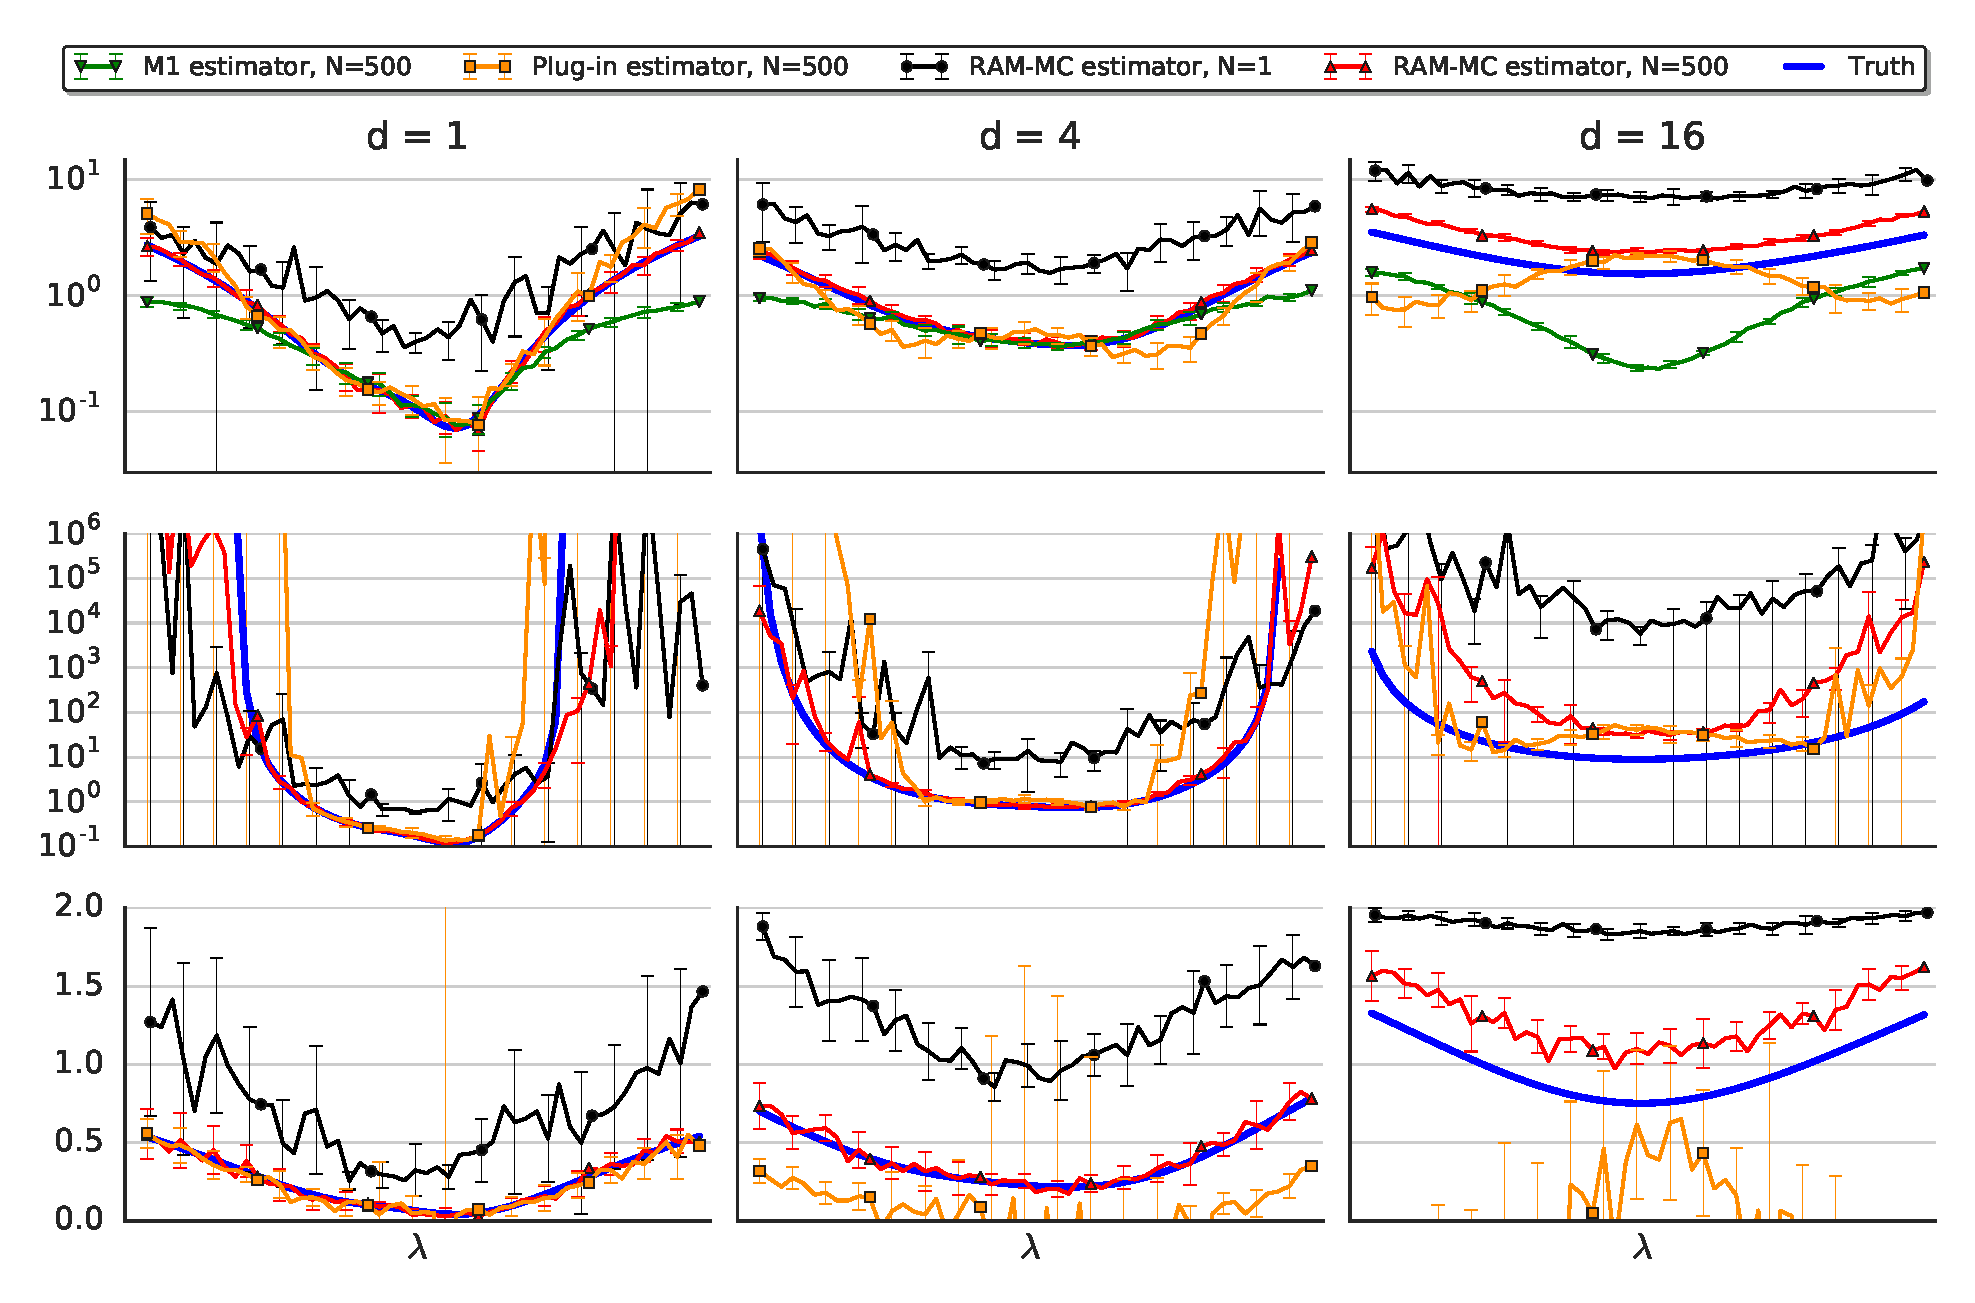
\includegraphics[width=0.97\textwidth, height=0.615\textwidth]{pics/NeurIPS_toy_exps_plot.pdf}};
\node[rotate=0] at (0, 1.7) {$\mathrm{H}^2$};
\node[rotate=0] at (0, 4.2) {$\chi^2$};
\node[rotate=0] at (0, 6.7) {$\mathrm{KL}$};
\end{tikzpicture}
\end{center}
\caption[Evaluation of RAM-MC on synthetic data]{\label{fig:synthetic-exps}
Results of synthetic experiments, Section~\ref{section:synth-exps}.
Estimating $D_f\bigl(\mathcal{N}(\mu_\lambda, \Sigma_\lambda),\, \mathcal{N}(0, I_d)\bigr)$ for various $f$, $d$, and parameters $\mu_\lambda$ and $\Sigma_\lambda$ indexed by $\lambda\in \R$.
Horizontal axis correspond to $\lambda\in[-2, 2]$,
columns to $d\in\{1, 4, 16\}$ and
rows to KL, $\chi^2$, and $\mathrm{H}^2$ divergences respectively.
{\bf \textcolor{blue}{Blue}} are true divergences, 
{\bf black} and {\bf \textcolor{red}{red}} are RAM-MC estimators (Equation \ref{eq:our-mc-estimate}) for $N\in\{1, 500\}$ respectively,
{\bf \textcolor{darkgreen}{green}} are M1 estimator of~\citep{nguyen10ratio} and {\bf \textcolor{orange}{orange}} are plug-in estimates based on Gaussian kernel density estimation \citep{moon14ensemble}.
$N=500$ and $M=128$ in all the plots if not specified otherwise.
Error bars depict one standard deviation over 10 experiments.
}
\end{figure}
\clearpage
}


% and used $\lambda \in [-2,2]$.

%
%Specifically, take ${P_Z} = $ and ${Q_X}$ to be standard normal distributions over $\Z=\R^d$ and $\X=\R^{20}$ respectively,
%and $\smash{Z\sim Q^\lambda_{Z|X}}$ to be a linear transform of $X$ plus a fixed isotropic Gaussian noise, with the linear function parameterised by $\lambda$.
%
%By varying $\lambda$ we can interpolate between different values for $D_f(Q_Z^\lambda , P_Z)$.

%\textbf{The estimators.}
Figure \ref{fig:synthetic-exps} shows the behaviour of RAM-MC with $N\,{\in}\,\{1, 500\}$ and $M{=}128$ compared to the ground truth as $\lambda \in [-2, 2]$ is varied. 
The columns of Figure~\ref{fig:synthetic-exps} correspond to different dimensions $d\,{\in}\,\{1, 4, 16\}$, and rows to the $\KL$, $\chi^2$ and $\mathrm{H}^2$ divergences, respectively. 
For each column, the values of $A_0$ and $v$ were randomly sampled so that the distributions being compared are the same within columns and different between columns.
Two other baseline methods are included for comparison.
First, a plug-in method based on kernel density estimation \citep{moon14ensemble}.
Second, and only for the KL case, the M1 method of \cite{nguyen10ratio} based on density ratio estimation (see Section \ref{sec:literature-density-ratio-estimation}).

%\textbf{The experiment.}
To produce each plot, the following was performed 10 times, with the mean result giving the bold lines and standard deviation giving the error bars.
First, $N$ points $\XN$ were drawn from $Q_X$. 
Then $M{=}128$ points $\ZM$ were drawn from $\hat{Q}_Z^N$ and RAM-MC (Equation \ref{eq:our-mc-estimate}) was evaluated. 
For the plug-in estimator, the densities $\hat{q}(z)$ and $\hat{p}(z)$ were estimated by kernel density estimation with 500 samples from $Q_Z$ and $P_Z$ respectively using the default settings of the Python library {\texttt{scipy.stats.gaussian\_kde}}.
The divergence was then estimated via MC-sampling using $128$ samples from $Q_Z$ and the surrogate densities.
The M1~estimator involves solving a convex linear program in $N$ variables to maximise a lower bound on the true divergence, see \cite{nguyen10ratio} for more details.
Although the M1~estimator can in principle be used for arbitrary $f$-divergences, its implementation requires hand-crafted derivations that are supplied only for the $\KL$ in \cite{nguyen10ratio}.

%\textbf{Discussion.}
The results of this experiment empirically support Proposition \ref{prop:upper-bound} and Theorems \ref{thm:fast-KL-rate}, \ref{thm:convergence-rate-general}, and~\ref{thm:mc-variance}:
(i) in expectation, RAM-MC upper bounds the true divergence; (ii) increasing $N$ from 1 to 500 clearly decreases both the bias and the variance of RAM-MC.
When the dimension $d$ increases, the bias for fixed $N$ also increases.
This is consistent with the theory in that, although the rates are independent of $d$, the constants are not.
By side-stepping the issue of density estimation, RAM-MC performs favourably compared to the plug-in and M1 estimators, more so in higher dimensions ($d=16$).
In particular, the shape of the RAM-MC curve follows that of the truth for each divergence, while that of the plug-in estimator does not for larger dimensions.
In some cases the plug-in estimator can even take negative values due to the large variance.




\subsection{Real-data experiments}
\label{sec:exp_wae}
%\textbf{The data model.}
To investigate the behaviour of RAM-MC in a more realistic setting, this experiment considers the estimation of divergences in the context of Variational Autoencoders (VAEs) and Wasserstein Autoencoders (WAEs), introduced in Section \ref{sec:literature-gen-models}.
Recall that both models have a prior ${P_Z}$ over the latent space and involve learning an encoder $\smash{Q^\phi_{Z|X}}$ with parameter $\phi$ mapping from the data to latent space.
%RAM-MC is used to estimate the divergence $D_f(Q^\phi_Z,P_Z)$ between the aggregate posterior and prior.
%A prior distribution ${P_Z}$ is specified, and the 
%optimization objectives of both models are of the form ``reconstruction + distribution matching penalty''.
%The penalty of the VAE was shown by \cite{hoffman2016elbo} to be equivalent to $\smash{\KL(Q^\theta_Z \| P_Z) + I(X,Z)}$ where $I(X,Z)$ is the mutual information of a sample and its encoding.
%The WAE penalty is ${D(Q^\theta_Z \| P_Z)}$ for any divergence $D$ that can practically be estimated.
%Following \cite{tolstikhin2017wasserstein}, we trained models using the Maximum Mean Discrepency (MMD), a kernel-based distance on distributions, and a divergence estimated using a GAN-style classifier leading to WAE-MMD and WAE-GAN respectively \cite{gretton2012kernel, goodfellow2014generative}.
% Both of them can be estimated from samples.
%For more information about VAE and WAE, see Appendix \ref{appendix:intro-vae-wae}.
%\textbf{The experiment.}

Pre-trained models that were trained on the \emph{CelebA} dataset \citep{liu2015faceattributes} were used to evaluate the RAM-MC estimator as follows.
The test dataset is taken as the ground-truth $Q_X$, and this is embedded into the latent space via the trained encoder.
Since all models considered have Gaussian encoders, the resulting \emph{empirical aggregate posterior}
is a ${\sim}{20}\text{k}$-component Gaussian mixture for $Q_Z$, one component for each item in the test dataset. 
Since $Q_Z$ is a finite---not continuous---mixture, the true $D_f(Q_Z,P_Z)$ can be estimated using a large number of MC samples ($10^4$ samples were used).
This is computationally costly as it involves evaluating $2\cdot 10^4$ Gaussian densities for each of the $10^4$ MC points.
This evaluation was repeated 10 times, and the means and standard deviations are reported in Figures \ref{fig:real-exps} and \ref{fig:real-exps-hsq} for the KL and $\mathrm{H}^2$ divergences respectively.
RAM-MC is evaluated using $N \in \{2^0, 2^1,\ldots, 2^{14}\}$ and $M \in \{10, 10^3\}$.
For each combination $(N,M)$, RAM-MC was computed 50 times with the means plotted as bold lines and standard deviations as error bars.
This procedure was performed for the KL and $\Hsq$ divergences on six models that were chosen to have latent dimension $d\in\{32, 64, 128\}$ and were selected from the classes VAE, WAE-MMD and WAE-GAN.

\afterpage{%
\begin{figure}
\begin{center}
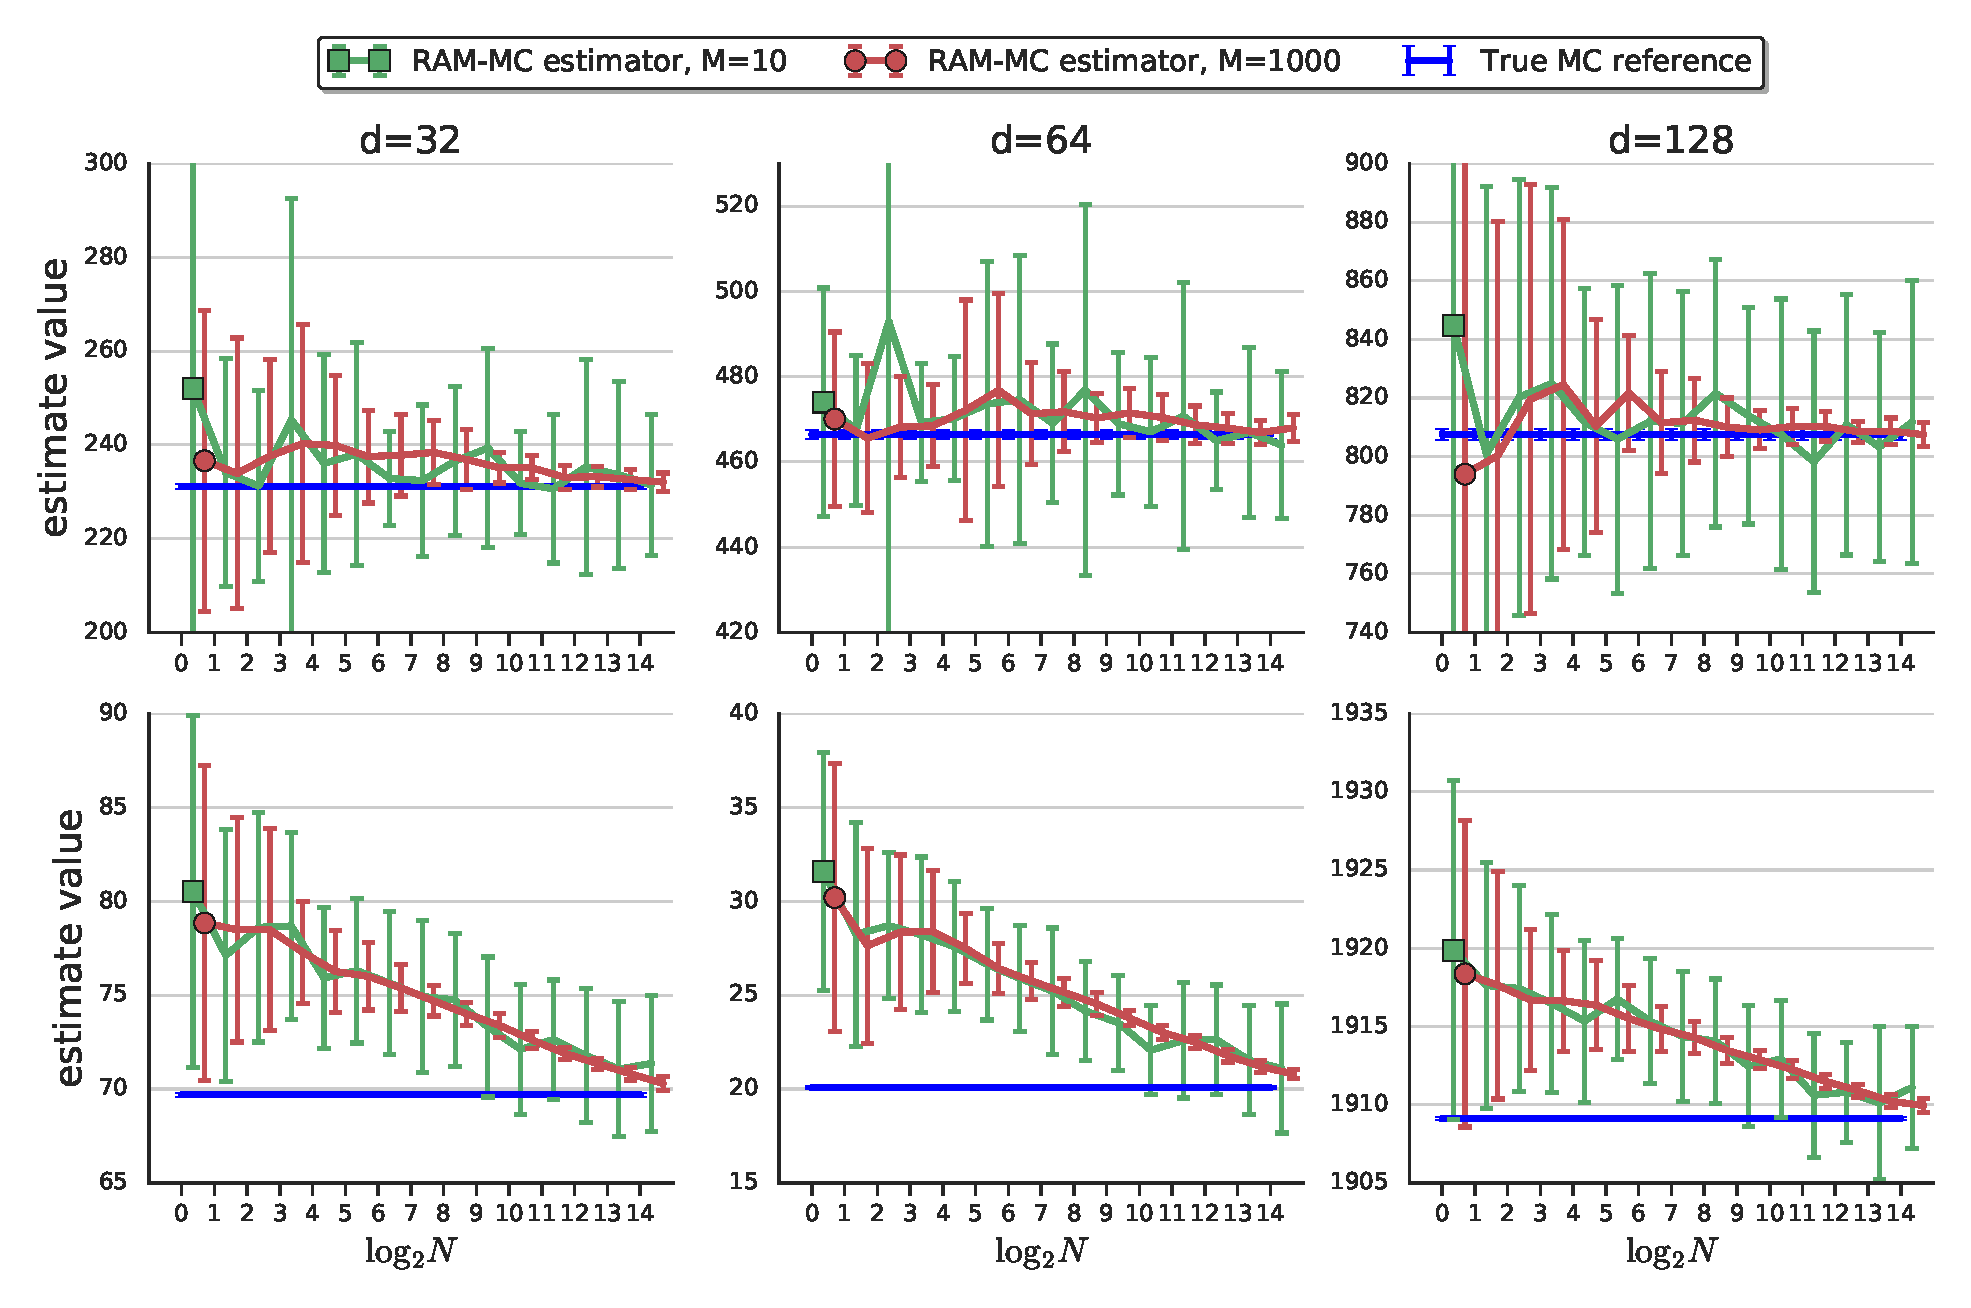
\includegraphics[width=1.\textwidth, height=0.615\textwidth]{pics/NeurIPS_wae_exps_plot.pdf}
\end{center}
\caption[Evaluation of RAM-MC on real data with KL-divergence]{\label{fig:real-exps}
Results of real-data experiments, Section~\ref{sec:exp_wae}. Estimates of $\KL(Q_Z^\theta , P_Z)$ for pretrained autoencoder models with RAM-MC as a function of $N$ for $M{=}10$ ({\bf \textcolor{green!65!blue}{green}}) and $M{=}1000$ ({\bf \textcolor{red}{red}}) compared to an accurate MC estimate of the ground truth ({\bf\textcolor{blue}{blue}}).
Lines and error bars represent means and standard deviations over 50 trials.
}
\end{figure}
\clearpage
}


\afterpage{%
\begin{figure}
\begin{center}
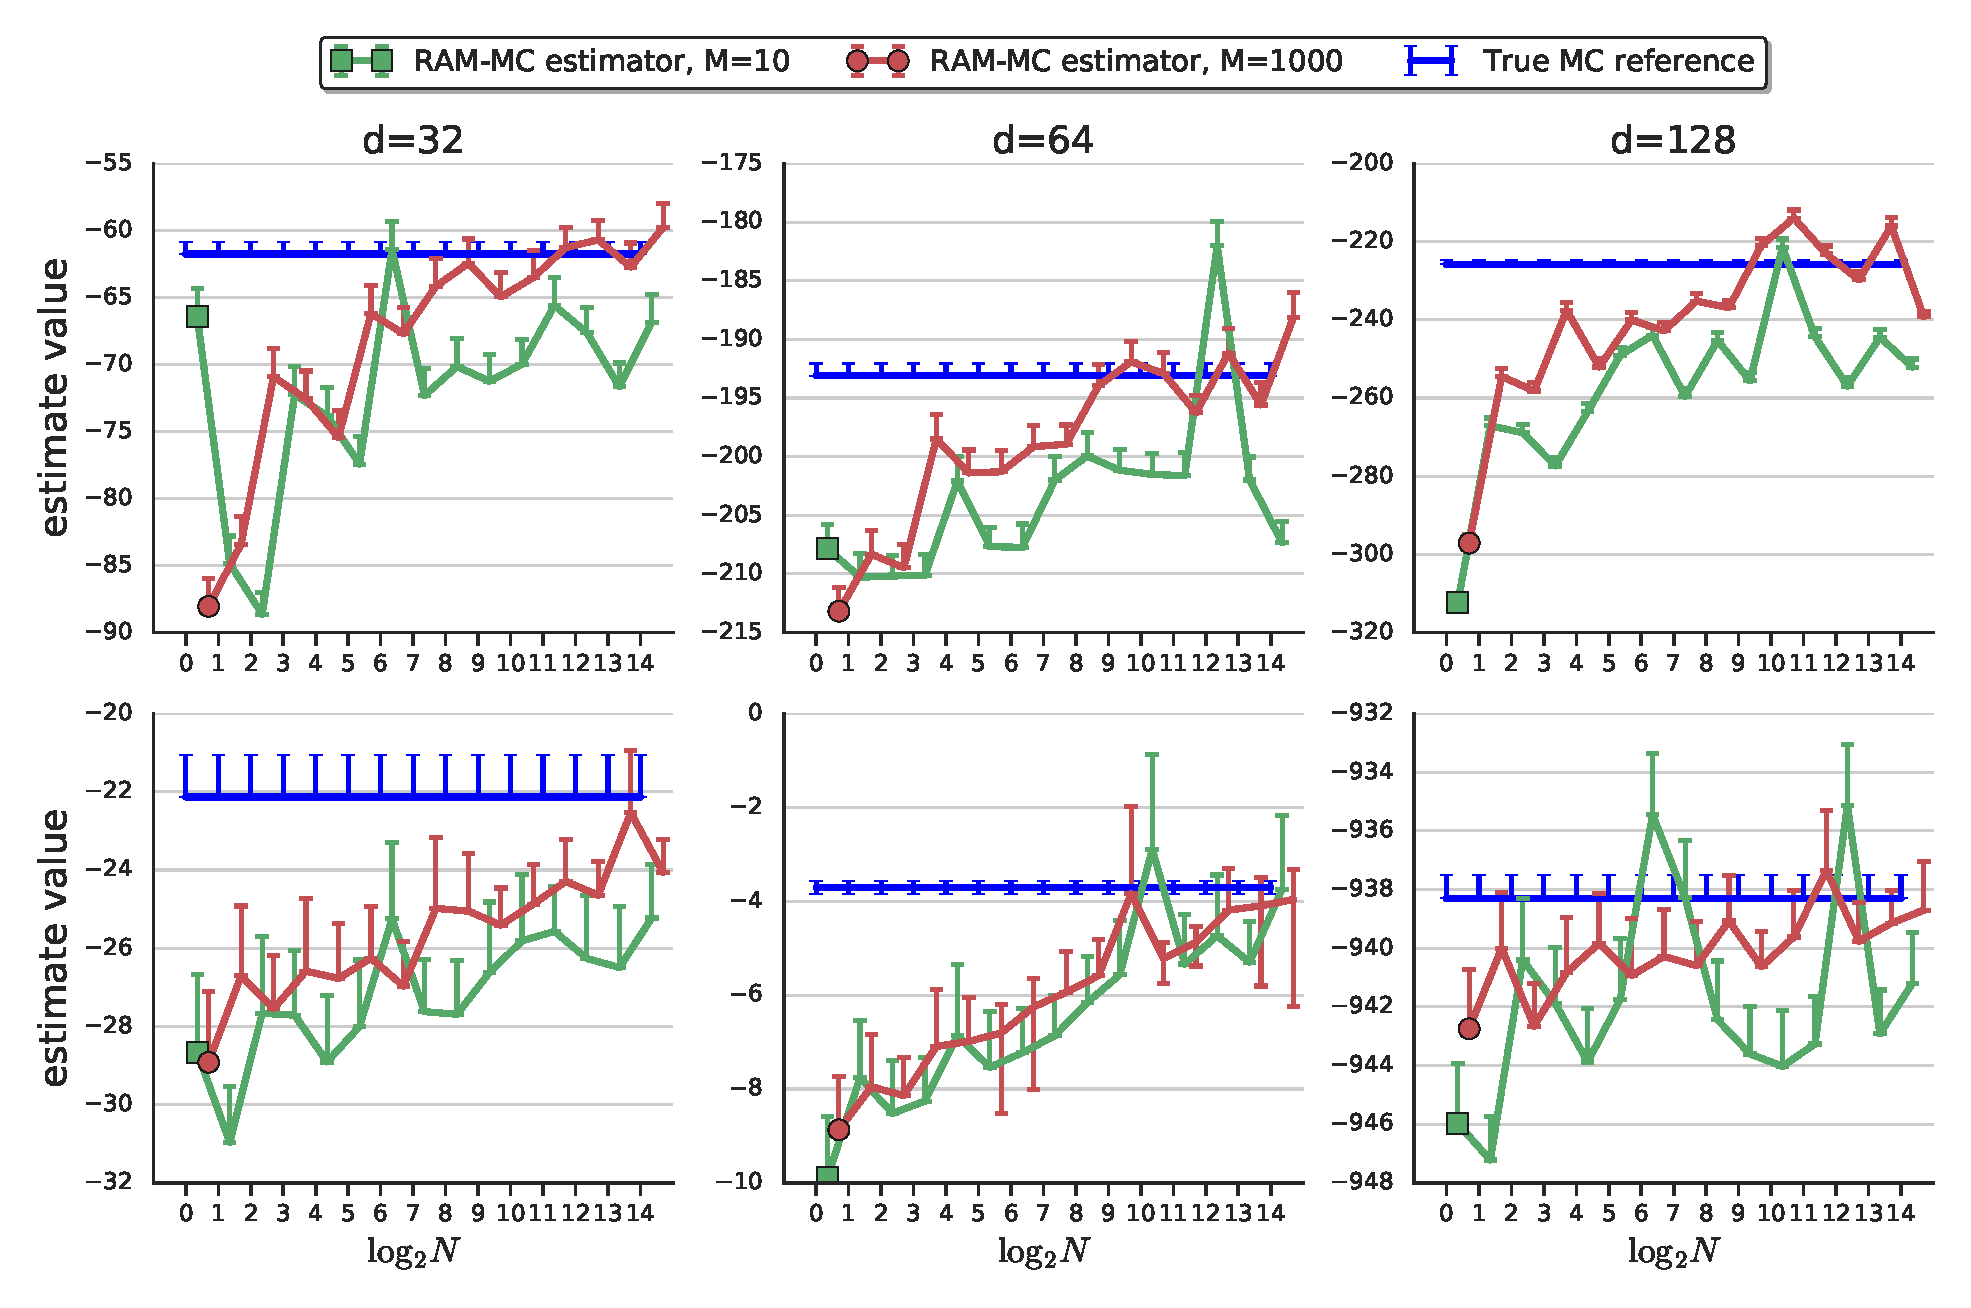
\includegraphics[width=1.\textwidth, height=0.615\textwidth]{pics/NeurIPS_wae_exps_plot_hsq.pdf}
\end{center}
\caption[Evaluation of RAM-MC on real data with $\Hsq$-divergence]{\label{fig:real-exps-hsq}
Results of real-data experiments, Section~\ref{sec:exp_wae}. Estimating $\Hsq(Q_Z^\theta , P_Z)$ in pretrained autoencoder models with RAM-MC as a function of $N$ for $M=10$ ({\bf \textcolor{green!65!blue}{green}}) and $M{=}1000$ ({\bf \textcolor{red}{red}}) compared to ground truth ({\bf\textcolor{blue}{blue}}).
Lines and error bars represent means and standard deviations over 50 trials.
Plots depict $\log\big(2 - \hat{D}^M_{\Hsq}(\hat{Q}^N_Z , P_Z)\big)$ since $\Hsq$ is close to 2 in all models.
Omitted lower error bars correspond to error bars going to $-\infty$ introduced by $\log$.
Note that the approximately \emph{increasing} behaviour evident here corresponds to the expectation of RAM-MC \emph{decreasing} as a function of $N$. 
Due to concavity of $\log$, the decrease in variance when increasing $M$ manifests itself as the {\bf \textcolor{red}{red}} line ($M{=}1000$) being consistently above the {\bf \textcolor{green!65!blue}{green}} line ($M{=}10$).
}
\end{figure}
\clearpage
}

Figure~\ref{fig:real-exps} shows the result of performing this for the KL divergence on six different models.
%For each dimension $d\in\{32, 64, 128\}$, two models were selected from the classes VAE, WAE-MMD and WAE-GAN. 
%See Appendix~\ref{appendix:real-data-experiments-additional} for further details and similar plots for the $H^2$-divergence.
%\textbf{Discussion.}
%The results are encouraging. 
In all cases RAM-MC achieves a reasonable accuracy with $N$ relatively small, even for the bottom right model where the true KL divergence ($\approx 1910$) is large.
There is evidence supporting Theorem~\ref{thm:mc-variance}, which informally states that the variance of RAM-MC is mostly determined by the smaller of $\psi(N)$ and $M$:
when $N$ is small, the variance of RAM-MC does not change significantly with $M$, 
however when $N$ is large, increasing $M$ significantly reduces the variance. 
It was found that there are two general modes of behaviour of RAM-MC across the six trained models considered. 
In the bottom row of Figure~\ref{fig:real-exps}, the decrease in bias with $N$ is very obvious, supporting Proposition~\ref{prop:upper-bound} and Theorems \ref{thm:fast-KL-rate} and \ref{thm:convergence-rate-general}.
In contrast, in the top row it is less obvious, because the comparatively larger variance for $M{=}10$ dominates reductions in the bias.
Even in this case, both the bias and variance of RAM-MC with $M{=}1000$ become negligible for large $N$.
Importantly, the behaviour of RAM-MC does not degrade in higher dimensions.

The baseline estimators (plug-in of \cite{moon14ensemble} and M1 of \cite{nguyen10ratio}) perform so poorly that 
%we decided not to include them in the plots (doing so 
their inclusion would distort the $y$-axis scale.
In contrast, even with a relatively modest $N{=}2^8$ and $M{=}1000$ samples, RAM-MC behaves reasonably well in all cases.

Figure~\ref{fig:real-exps-hsq} displays similar results for the $\Hsq$-divergence.
Since $\Hsq(A,B) \in [0, 2]$ for any probability distributions $A$ and $B$ and all computed estimates were close to $2$,
considerations of scale mean that the estimated values $\log\big(2 - \hat{D}^M_{\Hsq}(\hat{Q}^N_Z , P_Z)\big)$ were plotted instead.
Decreasing bias in $N$ of RAM-MC therefore manifests itself as the lines \emph{increasing} in Figure~\ref{fig:real-exps-hsq}. 
Concavity of $\log$ means that the reduction in variance when increasing $M$ results in RAM-MC with $M{=}1000$ being above RAM-MC with $M{=}10$.
Similar to the results for the KL, these also support the theoretical findings presented in the previous section.

Additionally, the same experiment was attempted using the $\chi^2$-divergence but numerical issues were encountered.
This can be understood as a consequence of the inequality $e^{\KL(A, B)} - 1 \leq \chi^2(A,B)$ for any distributions $A$ and $B$ (Lemma \ref{lemma:f-div-klleqchi}). 
From Figure~\ref{fig:real-exps} it can be seen that the $\KL$-divergence reaches values higher than $1000$, making the corresponding value of the $\chi^2$-divergence larger than can be represented using double-precision floats.






\section{Applications}\label{sec:applications}
This section details some direct consequences of the proposed estimator and its theoretical guarantees to existing literature, illustrating the applicability of this work.
%In addition, this theory may also apply to a number of machine learning domains where estimating entropy, total correlation or mutual information is either the final goal or part of a broader optimization loop.

\subsection{Entropy estimation}
The differential entropy, defined as $H(Q_Z)= -\int_{\mathcal{Z}} q(z) \log q(z)  dz$, is often a quantity of interest in machine learning.
While it is intractable in general, straightforward computation shows that for \emph{any} $P_Z$
{\addtolength{\abovedisplayskip}{-0.5mm}
\addtolength{\belowdisplayskip}{-0.5mm}
\begin{align*}
    H(&Q_Z) - \mathbb{E}_{\XN} H(\hat{Q}_Z^N) \\
    &= - \int q(z) \log q(z) dz + \mathbb{E}_{\XN} \int \hat{q}_N(z) \log \hat{q}_N(z) dz \\
    &= - \int q(z) \log q(z) dz + \int q(z) \log p(z) dz  \\
    & \qquad - \int \mathbb{E}_{\XN} \hat{q}_N(z) \log p(z) dz  + \mathbb{E}_{\XN} \int \hat{q}_N(z) \log \hat{q}_N(z) dz \\
    &= - \int q(z) \log \frac{q(z)}{p(z)} dz  + \mathbb{E}_{\XN} \int \hat{q}_N(z) \log \frac{\hat{q}_N(z)}{p(z)} dz \\
   	&= \mathbb{E}_{\XN} D_{\text{KL}}\left(\hat{Q}_Z^N , P_Z\right) -  D_{\text{KL}}\left(Q_Z , P_Z\right).
\end{align*}}
Therefore, Theorems \ref{thm:fast-KL-rate} and \ref{thm:convergence-rate-general} provide sufficient conditions under which $\smash{H(\hat{Q}_Z^N)}$ is an asymptotically unbiased estimator of $\smash{H(Q_{Z})}$.
Note that it suffices for the assumptions of these results to hold for \emph{any} choice of $P_Z$, suggesting that a more direct analysis of the behaviour of $\smash{H(\hat{Q}_Z^N)}$ could yield milder sufficient conditions.


\subsection{Total correlation estimation}
The results on entropy estimation have consequences for some existing VAE literature.
The Total Correlation (TC) of a distribution $Q_Z$, defined in terms of the KL-divergence, can be written in terms of differential entropy: 
%
\begin{align*}
TC(Q_Z) &:= D_{\text{KL}}\left(Q_Z, \prod_{i=1}^{d_Z} Q_{Z_i}\right)  \\
&= - \int q(z) \log \left( \frac{q(z)}{\prod_i q(z_i)} \right) dz \\
&= - \int q(z) \log q(z) dz + \int q(z) \sum_i \log q(z_i) dz \\
&= - \int q(z) \log q(z) dz + \sum_i \int q(z_i)  \log q(z_i) dz \\
&= \sum_{i=1}^{d_Z}H(Q_{Z_i}) - H(Q_Z)
\end{align*}
%
where $Q_{Z_i}$ is the $i$th marginal of $Q_Z$.
This is considered by \cite{chen2018isolating}, who subtract it from the VAE loss function (see Section \ref{sec:literature-gen-models}). 
Since a non-negative quantity is subtracted from a lower bound on the evidence, the resulting loss function is still an evidence lower bound, with additional encouragement for $Q_Z$ to be factorised. This is named the $\beta$-TC-VAE algorithm.
By the identities above, estimation of TC can be reduced to estimation of $H(Q_Z)$ with only slight modifications needed to treat $H(Q_{Z_i})$.

Two methods are proposed by \cite{chen2018isolating} for estimating $\smash{H(Q_Z)}$, both of which assume a finite dataset of size $D$.
One of these, named \emph{Minibatch Weighted Sample} (MWS), coincides with $\smash{H(\hat{Q}_Z^N) + \log D}$ estimated with a particular form of MC sampling.
The results presented in this chapter therefore imply \emph{inconsistency} of the MWS method due to the constant $\log D$ offset. 
This inconsistency is fact not problematic in the context of \cite{chen2018isolating} since they are concerned with minimising (not estimating) the TC, and a constant offset does not affect gradient-based optimization techniques.
Interestingly, although their derivations suppose a data distribution of finite support, the results presented here show that minor modifications result in an estimator suitable for both finite and infinite support data distributions.

\subsection{Mutual information estimation}
The mutual information (MI) between variables with joint distribution $\smash{Q_{Z,X}}$ is defined as 
\begin{align*}
\smash{I(Z, X) := D_{\text{KL}}\left(Q_{Z,X}, Q_Z Q_X \right) = \E_{X} D_{\text{KL}}\left(Q_{Z|X}, Q_Z \right)}.
\end{align*}

Several recent papers have estimated or optimised this quantity in the context of autoencoder architectures, coinciding with the setting considered here \citep{hoffman2016elbo, alemi2017fixing, dieng2018avoiding}. 
In particular, \cite{poolevariational} propose the following estimator based on replacing $Q_Z$ with $\smash{\hat{Q}_{Z}^N}$, proving it to be a lower bound on the true MI:
%
\begin{align*}\textstyle
    I_{TCPC}^N(Z,X) = \mathbb{E}_{\XN}\Big[\frac{1}{N} \sum_{i=1}^N D_{\text{KL}}\left( Q_{Z|X_i}, \hat{Q}_{Z}^N \right)\Big] \leq I(Z,X).
\end{align*}
%
The gap in this inequality can be written as
%
\begin{align*}
I(Z,X) - I_{TCPC}^N(Z,X) = \E_{\XN} D_{\text{KL}}\left( \hat{Q}_{Z}^N, P_{Z} \right) - D_{\text{KL}}\left( Q_{Z}, P_Z \right)
\end{align*}
%
where $P_Z$ is \emph{any} distribution. 
Therefore, the results in this chapter also provide sufficient conditions under which $\smash{I^N_{TCPC}}$ is an asymptotically unbiased estimator of the true mutual information.


%\todo{Rewrite section heading to make this next bit fit in, moved from the intro}
\subsection{Related, but fundamentally different work}
\cite{burda2015importance} propose to reduce the gap introduced by Jensen's inequality in the derivation of the classical ELBO by using multiple Monte-Carlo samples from the approximate posterior $\smash{Q_{Z|X}}$.
This is similar in flavour to the approach considered in this chapter, but is fundamentally different since the approach taken here uses multiple samples from the \emph{data distribution} to reduce a different Jensen gap.

To avoid confusion, note that replacing the `regulariser' term $\mathbb{E}_X[D_{\text{KL}}(Q_{Z|X}, P_Z)]$ of the classical ELBO with expectation of the proposed estimator $\E_{\XN}[D_{\text{KL}}(\hat{Q}_Z^N, P_Z)]$ results in an upper bound of the classical ELBO (by Proposition~\ref{prop:upper-bound}) but is itself not in general an evidence lower bound:
%
\begin{align*}
    \mathbb{E}_X \Big[ \mathbb{E}_{Q_{Z|X}} \log p(X|Z) - D_{\text{KL}}(Q_{Z|X}, P_Z ) \Big] \leq \mathbb{E}_X \Big[ \mathbb{E}_{Q_{Z|X}} \log p(X|Z) \Big] - \mathbb{E}_{\XN} \Big[ D_{\text{KL}}(\hat{Q}_Z^N, P_Z ) \Big].
\end{align*}


\section{Conclusion}\label{sec:conclusion}
This chapter introduced a practical estimator for the $\smash{f}$-divergence $D_f(Q_Z,P_Z)$ where $Q_Z = \int Q_{Z|X}dQ_X$, samples from $Q_X$ are available, and $P_Z$ and $Q_{Z|X}$ have known density.
The RAM estimator is based on approximating the true $Q_Z$ with data samples as a random mixture via $\smash{\hat{Q}^N_{Z}=\frac{1}{N}\sum_{n} Q_{Z|X_n}}$,
and RAM-MC is the version of this estimator where $\smash{D_f(\hat{Q}^N_Z,P_Z)}$ is estimated with MC sampling.

Rates of convergence and concentration were proved for both RAM and RAM-MC, in terms of sample size $N$ and MC samples $M$ under a variety of choices of $\smash{f}$.
Due to the strong structural assumptions made on the forms of the distributions in question, the fast rates presented here hold under relatively mild and verifiable further assumptions, thus making them applicable to the estimation of divergences in the latent spaces of autoencoders.
In contrast, in the existing literature on $f$-divergence estimation, which generally makes few structural assumptions, fast rates are only obtained under strong assumptions on the smoothness of densities or density ratios of the distributions. 

Synthetic and real-data experiments strongly support the validity of the proposal in practice, and the theoretical results provide guarantees for methods previously proposed heuristically in existing literature for mutual information and total correlation estimation,
thus extending understanding of the conditions under which these quantities can be estimated with practical numbers of samples.


Future work should investigate the use of the proposals for optimization loops, in contrast to pure estimation.
When $\smash{Q^\phi_{Z|X}}$ depends on parameter $\phi$ and the goal is to minimise $\smash{D_f(Q_Z^\phi , P_Z)}$ with respect to $\phi$, such as is the case for Wasserstein Autoencoders, RAM-MC provides a practical surrogate loss that can be minimised using stochastic gradient methods.






%!TEX root = ../thesis.tex
%*******************************************************************************
%****************************** Third Chapter **********************************
%*******************************************************************************

\newcommand\independent{\protect\mathpalette{\protect\independenT}{\perp}}
\def\independenT#1#2{\mathrel{\rlap{$#1#2$}\mkern2mu{#1#2}}}


\chapter{Multi-view Nonlinear Independent Component Analysis}\label{chapter:ica}

% **************************** Define Graphics Path **************************
\ifpdf
    \graphicspath{{Chapter4/Figs/Raster/}{Chapter4/Figs/PDF/}{Chapter4/Figs/}}
\else
    \graphicspath{{Chapter4/Figs/Vector/}{Chapter4/Figs/}}
\fi

\emph{%
This chapter presents identifiability results in a novel multi-view nonlinear ICA setting.
In the usual single-view setting, identifiability holds only under strong assumptions on the source distribution and mixing function.
The results presented here show that when multiple distinct views of the sources are available, identifiability holds under much weaker assumptions.
This work is an important contribution to the literature as it extends the few known identifiability results for nonlinear ICA models.}

%\emph{%
%Theorems \ref{thm:noiseless1} and \ref{thm:demixing} state that in contrast to the single-view setting, the two-view setting is identifiable when the mixing functions are arbitrary smooth, invertible nonlinear functions with smooth inverse, provided that one of the views is corrupted at the source level by sufficiently `complex' noise so that the Sufficiently Distinct Views assumption is satisfied.}
%
%\emph{Identifiability results are also obtained in the case of corruptions on both views. Theorem \ref{thm:two-noisy-views} states that the sources can be recovered up to the corruptions, and Corollary \ref{crl:lownoise} demonstrates that in limit as one of the corruptions becomes small, the uncorrupted sources can be recovered.}
%
%\emph{Finally, initial results are presented in Theorem \ref{thm:lastthm} providing conditions under which the uncorrupted sources are identifiable when a large number of views are available, even if these views are all corrupted by source noise.}



\emph{The main technical content of this chapter has been published in the paper:}

\begin{quote}
	\fullcite{gresele2019incomplete_fullcite}.
\end{quote}

%\emph{The Incomplete Rosetta Stone Problem: Identifiability Results for Multi-View Nonlinear ICA} published at UAI 2019.


\section{Introduction}

%\begin{itemize}
%	\item What is ICA?
%	\begin{itemize}
%		\item cocktail party problem with two speakers
%	\end{itemize}
%	\item Formal definition and definition of identifiability
%	\item Without making assumptions, identifiability is impossible (refer to nonlinear ica section for result)
%	\item Assumptions can be made on the mixing function or on the distribution of sources.
%	\item Discuss ambiguities at high level (identifiability usually is done up to 'tolerable ambiguities')
%\end{itemize}

Independent Component Analysis (ICA) is often motivated by the so-called \emph{cocktail-party problem}.
When two conversations at a party are happening simultaneously, a listener will hear different mixtures of the two audio streams produced by the speakers in each of their ears.
Despite both ears receiving mixtures of the conversations, the listener is able to focus on either of the conversations separately, hearing and understanding one while ignoring the other.
This is due to the brain's ability to separate out the mixed audio streams into the separate underlying sources, one for each conversation.

More generally, given data that are mixtures of independent underlying sources, the goal of ICA is `unmix' the data, thus recovering the sources.
This provides a principled approach to disentanglement of independent latent components, blind source separation, and feature extraction~\citep{hyvarinen2000independent}.
The applications of ICA are ubiquitous, including neuroimaging~\citep{mckeown1998independent}, signal processing~\citep{sawada2003direction}, text mining~\citep{honkela2010wordica}, astronomy~\citep{nuzillard2000blind} and financial time series analysis~\citep{oja2000independent}.

The ICA problem can be written formally by defining the 
latent variable model
%generative model
%\begin{align}
%\bm{x} &= \bm{f}(\bm{s}) \label{eqn:ica-basic-1}\\
%p(\bm{s}) &= \prod_{i} p_i(s_i) \label{eqn:ica-basic-2}
%\end{align}
%
\begin{align}
Z &\sim p(z) = \prod_i p(z_i) \label{eqn:ica-basic-1} \\
%Z &\sim P_Z = \prod_i P_{Z_i}  \\
X &= f(Z) \label{eqn:ica-basic-2}
%p(z) &= \prod_i p(z_i)
\end{align}
%
where $Z$ is a vector of independent \emph{sources}, $X$ is a vector of \emph{observations} or \emph{mixtures} and $f$ is the vector of \emph{mixing functions} expressing how each coordinate of $X$ depends on all of the coordinates of $Z$. 
Given a dataset of observations of $X$, the goal of ICA is to recover the corresponding unknown values of $Z$ by learning to invert the unknown $f$.
In the general case, no assumptions are made about $p(z)$ other than that it factorises.
The latent variable model in this setting should thus be thought of as a true descriptive model for the world, 
in contrast to generative modelling, where latent variable models with factorised priors merely provide a convenient way to specify distributions over the observable variables. 


%where $\bm{s}$ is a vector of independent \emph{sources}, $\bm{x}$ are the vector of \emph{observations} or \emph{mixtures} and $\bm{f}$ is the vector of \emph{mixing functions} expressing how each coordinate of $\bm{x}$ depends on all of the coordinates of $\bm{s}$. 
%%Generally, it is assumed that the number of sources and observations (i.e. the dimension of $\bm{s}$ and $\bm{x}$ respectively) are equal, which we will take to be the case throughout this chapter unless specified otherwise. 
%%If there are more observations than sources, the problem is called \emph{overdetermined} or \emph{undercomplete}, while if there more sources than observations it is called \emph{underdetermined} or \emph{overcomplete} \cite{citation_needed}.
%Given a dataset of observations of $\bm{x}$, the goal of ICA is to recover the corresponding unknown values of $\bm{s}$ by learning to invert the unknown $\bm{f}$.

An ICA problem is known as \emph{identifiable} when it is possible to recover the sources $Z$ up to tolerable ambiguities. 
For instance, it is generally acceptable to recover $Z$ up to linear rescaling or permuted coordinates.
Although identifiability results generally assume access to unlimited samples of data, they are crucial to ensuring the reliability of ICA methods in practical scenarios; in the absence of these, there is no guarantee that a proposed method will successfully reconstruct the true sources, even in controlled settings.

It was proven by \cite{hyvarinen1999nonlinear} that the `vanilla' ICA setting, in which only independence of the sources and invertibility of $f$ are assumed, is \emph{non-identifiable}.
Thus, much of the research in this field has attempted to characterise the assumptions under which identifiability holds.
Such assumptions may be made either on the mixing functions or on the distributions of the sources. 


\begin{figure}
\center

\end{figure}

\begin{figure}
	\begin{subfigure}{.45\linewidth}
		\center\
		\begin{tikzpicture}
		\node[icavarobs] (X) at(0,-2) {$X$};
		\node[icavar] (Z) at(0,0) {$Z$};
		\draw[->] (Z) -- (X);
		\end{tikzpicture}
		\caption{}\label{fig:ica-model:a}
	\end{subfigure}
	%
	\hfill
	%
	\begin{subfigure}{.45\linewidth}
		\center\
		\begin{tikzpicture}
		\node[icavar] (Z) at(0,0) {$Z$};
		\node[icavarobs] (X1) at(-1,-2) {$X_1$};
		\node[icavarobs] (X2) at(1,-2) {$X_2$};
		\draw[->] (Z) -- (X1);
		\draw[->] (Z) -- (X2);
		\end{tikzpicture}
		\caption{}\label{fig:ica-model:b}
	\end{subfigure}
	%
	\caption{Graphical models depicting (a) the usual single-view ICA setting; (2) the multi-view setting considered in this work. $Z$ is a vector of unobserved latent sources and the $X_i$ are observed mixtures of the components of $Z$.}
\end{figure}


The central contribution of the work presented in this chapter is the derivation of identifiability results in a novel \emph{multi-view} setting, in which multiple observations of the same underlying sources through different mixing functions are given (see Figure \ref{fig:ica-model:b}):
%
\begin{align*}
Z &\sim \prod_i p(z_i) \\
X_1 &= f_1(Z) \\
X_2 &= f_2(Z)
\end{align*}
%
In this setting, identifiability holds subject to much weaker assumptions than are required for the single-view setting.
These results are of practical importance for applications in which multiple data modalities may be simultaneously available.

For a high-level intuition of the results, consider the perception of 3D structure through eyesight.
Each of our eyes only sees a 2D projection of the true state of the 3D world.
With only a single eye available, it may be possible to infer the 3D structure present in a scene by exploiting known cues, such as the objects in the scene being familiar to the viewer or the presence of shadows.
But with two eyes together, a human can perceive 3D structure immediately, even without such cues. 
Analogously, the results presented in this work show that inference of latent structure can be performed under much weaker assumptions when more than a single view is available.


The remainder of this chapter is structured as follows.
Section \ref{sec:ica-literature-overview} provides an introduction to ICA and the literature surrounding it, as well as literature from other areas that is relevant to the setting considered in this work.
Section \ref{sec:ica-nonlinear-ica-with-mulitple-views} presents the main results.
Section \ref{sec:ica-assumptions} discusses the assumptions we make, and Section \ref{sec:on_suffistv} concludes.


%In the rest of this section we give an overview of the different cases for which identifiability results are known. 
%%Note that the ICA literature also includes a variety of methods for implementing solutions to the problem with real data, as well as a variety of application areas. 
%%Since the contribution of this chapter is to prove identifiability results in a novel setting, only the essentials required to understand the novel results in full context will be provided in this section.
%In brief, the case of linear mixing functions has been extensively studied and is well understood, while the non-linear case is more challenging.
%Recently, many papers have used a novel proof technique to derive identifiability results in slight modifications to the standard ICA problem setting.
%The contribution of this chapter (Sections ??-??) is similar, proving identifiability in the case of \emph{multiple nonlinear views}. 
%That is, the given dataset consists of observations $\bm{x}^{(1)}$ and $\bm{x}^{(2)}$ of the same sources $\bm{s}$.

%\emph{Notation: discuss use of bold lower case letters for vectors in usual ICA literature and that here we use capitals for consistency with rest of thesis.}

\section{Overview of ICA and related literature}\label{sec:ica-literature-overview}

This section provides an overview of different ICA settings for which identifiability results are known, and discusses other literature relevant to the multi-view setting considered in this work.


%Sections \ref{subsec:ica-literature-linear-ica} - \ref{subsec:ica-literature-nonlinear-ica-with-aux} provide an overview of different ICA settings for which identifiability results are known.
%In brief, the linear case has been extensively studied and is well understood, while the nonlinear case is more challenging.
%Recently, a novel proof technique has been used to derive identifiability results in slight modifications to the standard ICA problem setting.
%Section \ref{sec:related-work} discusses other literature that is not about ICA but is nonetheless relevant to the setting considered in this work.



\subsection{Linear ICA}\label{subsec:ica-literature-linear-ica}

%\begin{itemize}
%	\item The linear case has been studied extensively and is identifiable if at most one of the components is Gaussian
%	\item If more than one component is Gaussian, then these components cannot be unmixed since Gaussians are closed under linear mixing, so any linear unmixing function will not be able to distinguish them.
%	\item Overview of techniques
%\end{itemize}

Linear ICA refers to the setting in which the vector of mixing functions $f$ is a linear map, 
in which case the ICA model can be written
%
\begin{align*}
Z &\sim \prod_i p(z_i) \\
X &= AZ
\end{align*}
%
where $A$ is a square matrix.
This problem has been extensively studied and has been shown to be identifiable if at most one of the latent components is Gaussian~\citep{darmois1953analyse, skitovich1954linear, comon1994independent}.
Nonidentifiability in the case of more than one Gaussian component is a consequence of the fact that an isotropic Gaussian is invariant under orthogonal linear mappings.
Thus if the diagonal matrix $\Lambda$ rescales the Gaussian components of $Z$ to be unit variance, and $U$ is an orthogonal matrix mixing these components, $X$ can be rewritten
%
\begin{align*}
X = \left(A\Lambda^{-1}U^{-1} \right) \left(U\Lambda Z\right).
\end{align*}
%
Since both $Z$ and $U\Lambda Z$ have independent components, it is impossible to tell which of $Z$ and ${U}{\Lambda} Z$ corresponds to the true source distribution.
For most such $U$, $U\Lambda Z$ nontrivially mixes the components of $Z$, and thus the problem is nonidentifiable due to the existence of multiple plausible, yet fundamentally different, solutions.

Note that even in the non-Gaussian case, taking $U=I$ or a permutation matrix also results in $U\Lambda Z$ being a valid solution. 
This, however, corresponds to a `trivial' indeterminacy of the linear ICA problem, since in this case $U\Lambda Z$ still recovers the separate components of $Z$, only linearly rescaled and in a different order.

The non-Gaussianity assumption is exploited by linear ICA algorithms by seeking linear maps $W$ such that the transformed data ${W}X$ have maximally non-Gaussian components.
Intuition for why such an approach works can be seen in the Central Limit Theorem, which, informally, states that an average of \iid~random variables becomes more Gaussian-like as the number of variables in the average increases. 
Similarly, in sense that can be made formal \citep{hyvarinen2000independent}, linearly mixing random variables makes them more Gaussian-like, meaning that appropriate measures of Gaussianity can be used as objective functions for de-mixing.

We recall in passing that linear ICA methods can be used for causal discovery in linear cyclic models, as discussed in Section \ref{subsubsec:causality-causal-inference-cyclic}.\footnote{\todo{rewrite if order of chapters is changed}}





\subsection{Nonlinear ICA}\label{subsec:ica-literature-nonlinear-ica}
 
It was proved by \cite{hyvarinen1999nonlinear} that if only independence of the sources and invertibility of $f$ are assumed, the nonlinear ICA problem is unidentifiable.
Specifically, given any distribution over the observable variables $X$ that admits density with respect to Lebesgue measure, there exist many vector-valued invertible mappings $g$ with the property that the components of $g(X)$ are independent, and these many solutions are non-trivially different.
%i.e. their differences are more than the permutation or linear rescaling indeterminacy of the linear case.

This is proved by first demonstrating the existence of a function $g$ with the property that $Y=g(X)$ is uniformly distributed on the unit cube $[0, 1]^n$,
a generalisation of the result that, for a one-dimensional random variable $U$  with cumulative distribution function $F_U$, the random variable $F_U(U)$ is uniformly distributed on $[0,1]$.
Next, non-uniqueness is proved by demonstrating the existence of an infinite class of functions $h$ which are \emph{measure-preserving} maps $[0,1]^n \to [0,1]^n$. 
That is, if $Y$ is uniformly distributed on $[0,1]^n$ then so is  $Y' = {h}({Y})$.
It follows that ${h}\circ {g}$ thus provides a valid solution to the nonlinear ICA problem and thus there are infinitely many solutions. 
Such a class of measure-preserving functions is given explicitly in the case of $n=2$ dimensions; by extending such functions to the identity mapping on extra dimensions and composing, such a class can be generated for any $n$.

%There are two main steps to this proof: first the existence of a solution is shown, after which it is demonstrated that it is not unique.
%These are briefly reviewed next.
%
%Existence of a solution is demonstrated by explicit construction.
%Given a vector of random variables $X \in \mathbb{R}^n$
%% whose distribution admits density with respect to Lebesgue measure
%, a function $g$ is constructed such that the random vector $Y = g(X) $ is uniformly distributed on the unit cube $[0, 1]^n$.
%${g}$ is constructed coordinate-wise in an iterative process that is similar to Gram-Schmidt orthogonalisation. See Theorem 1 of \cite{hyvarinen1999nonlinear} and the preceding paragraphs for details.
%$\bm{y}$ has independent components and, since this method works for any $\bm{x}$ with non-degenerate distribution, a solution to the ICA problem therefore always exists.
%
%Non-uniqueness of this solution is demonstrated by observing that there exists an infinite class of functions $\bm{h}$ which are \emph{measure-preserving} maps $[0,1]^n \to [0,1]^n$. 
%That is, if $\bm{y}$ is uniformly distributed on $[0,1]^n$ then so is  $\bm{y}' = \bm{h}(\bm{y})$.
%It follows that $\bm{h}\circ \bm{g}$ thus provides a valid solution to the nonlinear ICA problem and thus there are infinitely many solutions. 
%Such a class of measure-preserving functions is given explicitly in the case of $n=2$ dimensions; by extending such functions to the identity mapping on extra dimensions and composing, such a class can be generated for any $n$.

Note that any function ${k}: \mathbb{R}^n \to \mathbb{R}^n$ that acts coordinate-wise and is invertible---that is, for each $i$, ${k}(X)_i = k_i(X_j)$ for some $j$ with $k_i$ invertible---can be composed with ${g}$ to result in the random vector $Y'={k}\circ {g}(X)$ having any desired factorised distribution. 
This is in some sense a `trivial' indeterminacy of nonlinear ICA, analogous to the scalar and permutation indeterminacy of linear ICA.
All of the novel identifiability results presented in Section \ref{sec:ica-nonlinear-ica-with-mulitple-views} hold only up to such functions, which are referred to throughout as \emph{component-wise invertible transformations}.


Other works have shown that identifiability is possible when additional assumptions are made.
Mostly these assume that the observations correspond not to \iid~samples of the sources, but rather time series with temporal structure \citep{cardoso2001three, singer2008non, sprekeler2014extension}.
In contrast, \cite{taleb1999source} prove identifiability under the rather strong \emph{post-nonlinear mixing} assumption on the mixing functions, corresponding to linear mixing followed by a nonlinear component-wise invertible function.


%In the following section we discuss recent developments in the ICA literature that have led to identifiability results with arguably weaker assumptions.





%\begin{itemize}
%	\item Without making assumptions, identifiability is impossible.
%	\item In the past two decades some work has been done on this. Some works making assumptions on the sources as time series, some restricting the mixing function classes.
%\end{itemize}

\subsection{Nonlinear ICA with auxiliary variables}\label{subsec:ica-literature-nonlinear-ica-with-aux}

\cite{hyvarinen19a} study a modification of the typical ICA setting where an additional observed auxiliary variable $U$ is introduced.
$U$ is assumed to be always observed with the sources $Z$ being \emph{conditionally} independent given $U$, resulting in the model

%\begin{align}
%\bm{x} &= \bm{f}(\bm{s}) \\
%p(\bm{s}|\bm{u}) &= \prod_{i} p_i(s_i | \bm{u}).
%\end{align}

\begin{align}
Z | U &\sim p(z|u) = \prod_{i} p_i(z_i | u), \\
X &= f(Z).
\end{align}

%Crucially, the variables $\bm{u}$ are presumed to be observed. 
This general model includes temporally dependent sources as a special case, taking $(U, X)= (X_t,X_{t+1})$.
%For notational convenience later on, let $q_i(s_i, \bm{u}) = \log p_i(s_i | \bm{u})$.
\cite{hyvarinen19a} prove identifiability results under conditions on both the conditional distributions $p_i(z_i | u)$, the relationships between sources and auxiliary variables, and subject to $U$ having a sufficiently diverse influence on the $X$ in a sense that is formalised as the \emph{assumption of variability}.

Identifiability in this model is proved constructively by considering classification between tuples $(x, u)$, sampled from the joint distribution $p(x, u)$, and tuples $(x, u^*)$ sampled from the product of marginals $p(u)p(x)$.
Tuples from the former distribution correspond to the same value of the sources $z$, and thus share information, while tuples from the latter correspond to different sources and thus do not share information.
By appropriately constraining the form of the regression function used in this classification, it is shown that the optimal classifier extracts $z$ up to component-wise invertible functions.

The results presented in Section \ref{sec:ica-nonlinear-ica-with-mulitple-views} build on this approach, extending the results to a novel multi-view setting.

%A constructive proof of identifiability is attained by exploiting a technique known as \emph{contrastive learning}~\citep{gutmann2010noise}.
%This is a method to transform a density ratio estimation problem into one of supervised function approximation. This idea has a long history~\citep{friedman2001elements}, and has more recently attracted attention in machine learning the machine learning community \citep{goodfellow2014generative, gutmann2010noise}. 
%This will be discussed in more detail in the next chapter.\footnote{\todo{rewrite if chapters are moved or if separate literature review covering this is put at the beginning.}}

%In the setting of nonlinear ICA with auxiliary variables, contrastive learning can be exploited by training a classifier to distinguish between a tuple sampled from the joint distribution, which we denote as $(\bm{x}, \bm{u})$, and one where $\bm{u}^*$ is a sample generated from the marginal $p(\bm{u})$ independently of $\bm{x}$, $(\bm{x}, \bm{u}^*)$.\footnote{\todo{Discuss density estimation in earlier literature review and reference it here.}}
%Intuitively, tuples drawn from the former distribution correspond to the same sources $\bm{s}$, and thus share information, while tuples from the latter correspond to different sources and thus do not share information.
%Since the marginals of both distributions are equal, the classifier must learn to distinguish between them based on the common information shared by $\bm{x}$ and $\bm{u}$; that is, ultimately, $\bm{s}$.
%
%With this method, the reconstruction of $\bm{s}$ is again possible only up to invertible scalar ``gauge'' transformations. 


\subsection{Other related work}\label{sec:related-work}
A central concept of the work presented in this chapter is the extraction of features from multiple simultaneous views. 
This section briefly reviews some related work considering similar settings outside of the ICA literature.
\subsubsection{Canonical Correlation Analysis}
\label{sec:probacca}
Given two vector-valued random variables, the goal of Canonical Correlation Analysis (CCA) is to find a pair of linear subspaces that have high cross-correlation, so that each component within one of the subspaces is correlated with a single component from the other subspace~\citep{hotelling1992relations, bishop2006pattern}.
CCA admits a probabilistic interpretation \citep{bach2005probabilistic} and is equivalent to maximum likelihood estimation in a graphical model which is a special case of that depicted in Figure 
\ref{fig:ica-model:b}.

The main differences compared to the setting of this chapter are that the latent components retrieved in CCA are forced to be uncorrelated, whereas ICA is concerned with independent components; and in CCA, mappings between the sources and observations are linear, whereas this work considers nonlinear mappings.
In dealing with correlation instead of independence, CCA is more closely related to Principal Component Analysis (PCA) than to ICA.
Nonlinear extensions of the basic CCA framework have been proposed~\citep{lai2000kernel, fukumizu2007statistical, andrew2013deep, michaeli2016nonparametric}, but identifiability results in the sense considered in this work are lacking.


%

%At a high level, the two noisy views model we consider in Section \ref{sec:constrained} is to CCA as nonlinear ICA is to PCA.



\subsubsection{Multi-view latent variable models}


%Bearing a strong resemblance to our considered setting,~\cite{lederman2018learning} proposes a sequence of diffusion maps to find the common source of variability captured by multiple sensors, discarding irrelevant sensor-specific effects.
%It computes the distance among the samples measured by different sensors to form a similarity matrix for the measurements of each sensor; each similarity matrix is then associated to a diffusion operator, which is a Markov matrix by construction. A Markov chain is then run by alternately applying these Markov matrices on the initial state. During these Markovian dynamics, sensor specific information will eventually vanish, and the final state will only contain information on the common source.
%While the method focuses on recovering the common information in the form of a parametrisation of the common variable, our method both inverts the mixing mechanisms of each view and recovers the common latent variables.

\cite{song2014nonparametric} prove identifiability for multi-view, discrete latent variable models.
%, unifying previously proposed spectral techniques~\cite{anandkumar2014tensor}. 
While the setting they consider is similar to that of this work, their proposed method is aimed at estimating model parameters with the goal of performing density estimation, rather than estimating the values of (continuous) latent variables.
%However, while the setting is similar to the one considered in this work, both the objectives and the employed methods are different.
The paper considers a setting in which $L$ variables $X_l$, $l=1, \ldots, L$ are observed; additionally, there exists an unobserved discrete latent variable $H$, such that conditional distributions $P(X_l|H)$ are independent. 
Their method is based on the mean embedding of distributions in a Reproducing Kernel Hilbert Space and a result of identifiability for the parameters of the mean embeddings of $P(H)$ and $P(X|H)$ is proved.

Another related field of study is multi-view clustering, which considers a multiview setting and aims at performing clustering on a given dataset, see e.g.~\cite{de2005spectral} and~\cite{kumar2011co}. This line of work differs from the setting considered here in two key ways.
First, clustering can be thought of as assigning a discrete latent label per observation. 
In contrast, the setting considered here is concerned with recovery of a continuous latent vector for each observation.
Second, since no underlying generative model with discrete latent variables is assumed, identifiability results are not given.



\subsubsection{Half-sibling regression}
\label{sec:hsr}
Half-sibling regression \citep{scholkopf2016modeling} is a method to reconstruct a source from noisy observations by exploiting observations of other sources that are affected by the same noise process.
In contrast to the multi-view ICA setting, in which the sources to be reconstructed are common to the multiple views, in half-sibling regression it is the \emph{noise} that is common to both views, with the desired sources being separate for each observation.

\cite{scholkopf2016modeling} study this problem under an additive noise assumption. 
By regressing one observation against the other, this common noise can be identified and hence subtracted, recovering the desired sources.

%Suppose that a latent variable of interest $Q$ is not directly available, and that we can only observe corrupted versions of it, denoted as  $Y$, where the corruption is due to a noise $N$.
%Without knowledge of $N$, it is impossible to reconstruct $Q$. However, if one or more additional variables $X$, also influenced by $N$, are observed, we can exploit them to model the effect of $N$ on $Y$ by regressing $Y$ on $X$.
%
%Subtracting this from the observed $Y$ recovers the latent variable $Q$ up to a constant offset,
%provided that (1) the additivity assumption
%\[
%Y = Q + f(N)
%\]
%holds, and (2) that $Y$ contains sufficient information about $f(N)$.
%Analogous to our aim of recovering $\bm{s}$,
%the goal of half-sibling regression is not to infer only the distribution of $Q$, but rather the random variable itself (almost surely).

\section{Nonlinear ICA with multiple views}\label{sec:ica-nonlinear-ica-with-mulitple-views}

This section presents the main contribution of this chapter, in which identifiability results for variations on the following setting are given:
\begin{align}
Z &\sim p(z) = \prod_{i} p_i(z_i) \label{eq:firstind}\\
X_1 &= f_1(Z) \label{eq:nonlinear-ica-1}\\
X_2 &= f_2(Z) \label{eq:nonlinear-ica-2}
\end{align}
where $X_1, X_2, Z \in \mathbb{R}^D$ and $f_1, f_2$ are arbitrary smooth and invertible transformations of the latent variable $Z = (Z_1, \ldots, Z_D)$ with smooth inverse.
$X_1$ and $X_2$ are referred to as different \emph{views} of the sources $Z$.
Given observations of $X_1$ and $X_2$, the goal is to recover $Z$, undoing the mixing induced by the $f_i$.

%the goal is to recover $\bm{s}$, undoing the mixing induced by the $\bm{f}_i$, in the case where only observations of $\bm{x}_1$ and $\bm{x}_2$ are available.
%correspondingly build on the methods introduced in that work. 
%The main difference between the setting is that do not assume that the $\bm{s}$ are conditionally independent given one of the $\bm{x}_i$.
The two problems defined by separately considering the pairs of Equations \ref{eq:firstind}, \ref{eq:nonlinear-ica-1} and \ref{eq:firstind}, \ref{eq:nonlinear-ica-2} are instances of the usual single-view nonlinear ICA setting.
As previously discussed, unless strong assumptions are made on the $f_i$ or the distribution of $Z$, these problems are separately unidentifiable. 

The key contribution of this chapter is 
%to show that 
the derivation of
identifiability results 
%can be obtained 
with relaxed assumptions by exploiting the fact that the 
%the structure of the generative model, in which observations of the 
two views are connected through the shared latent variable $Z$. 
That is, observing $X_1$ and $X_2$ together provides sufficient information to remove the ambiguities present in the vanilla nonlinear ICA setting.



This section considers three instances of the general setting described above, providing identifiability results for each.
Specifically:
%
\begin{itemize}
	\item Section \ref{sec:onenoisless} considers the case that only one of the observations, $X_2$, is corrupted with noise, showing that it is possible to fully reconstruct $Z$ using the noiseless variable. 
	This corresponds to a setting in which one accurate measurement device is supplemented with a second noisy device. 
	\item Section \ref{sec:constrained} considers the case that both variables are corrupted with noise, showing that it is possible to recover $Z$ up to the corruptions. 
	Furthermore, it is shown that $Z$ can be recovered with arbitrary precision in the limit that the corruptions go to zero.
	\item Section \ref{sec:multiple} considers the case of $M$ simultaneous views of the source $Z$ rather than just two.
	When considering the limit $M \rightarrow \infty$, sufficient conditions are provided under which it is possible to reconstruct $Z$ even if each observation is corrupted by noise.
\end{itemize}
%
%To the best of our knowledge, no result of identifiability of latent sources in the case in which only corrupted, mixed versions are observed has been given before.


%We consider a contrastive learning task in which a classifier is trained to distinguish between pairs $(\bm{x}_1, \bm{x}_2)$ corresponding to the same $\bm{s}$ and $(\bm{x}_1, \bm{x}^*_2)$ corresponding to different realisations of $\bm{s}$.
%The classifier is forced to employ the information shared by the simultaneous views in order to distinguish the two classes.
%By placing constraints on the form of this classifier, this ultimately results in recovering $\bm{s}$ (up to unavoidable ambiguities).

The setting considered in this work is related to that of \cite{hyvarinen19a}, discussed in Section \ref{subsec:ica-literature-nonlinear-ica-with-aux},
and the approach to proving the identifiability results presented here builds on the technique presented in that work.
%A crucial difference between the two settings is that here it is not assumed that the sources $\bm{s}$ are conditionally independent given one of the $\bm{x}_i$.
This approach 
%to recovering $\bm{s}$ 
is to classify between pairs $(X_1, X_2)$ corresponding to the same $Z$ and $(X_1, X^*_2)$ corresponding to different realisations of $Z$.
This classification problem can only be solved by employing the information shared by the simultaneous views in order to distinguish the two classes.
By placing constraints on the regression function used in such a classifier, it can be shown that an intermediate layer recovers $Z$ up to unavoidable ambiguities.

For technical reasons discussed in Section
\ref{sec:converged}, the results require some stochasticity in the relationship between $Z$ and at least one of the $X_i$.
This is not a significant constraint in practice; in most real settings observations are corrupted by noise, and a truly deterministic relationship between $Z$ and the $X_i$ would be unrealistic.
Component-wise independent corruptions of the sources are considered, i.e. $\mathbb{R}^D$-valued noise vectors $N_1$ and $N_2$ are introduced, and $X_1 = f_1 \circ g_1(Z, N_1)$ with $g_{1i}(Z, N_1) = g_{1i}(Z_i, N_{1i})$, where the components of $N_{1}$ are mutually independent, and similar for $N_2$ and $X_2$. 
The noise variables $N_1$, $N_2$ and the sources $Z$ are assumed to be mutually independent.
This constrains the way the source is corrupted by noise, namely the $g_i$, and not the mixing functions $f_i$.
In the the vanilla ICA setting, inversion of the mixing function and recovery of the sources $Z$ are equivalent; in the setting considered here, inversion of the mixing $f_i$ only implies recovering the sources up to the effect of the corrupter $g_i$.

Such $g_i$ as described in the previous paragraph are referred to as \emph{component-wise corrupters} throughout, and the corresponding output as \emph{corruptions}. 
All identifiability results hold only up to \emph{component-wise invertible transformations}, meaning that the components of $Z$ are recovered, but possibly reparametrised and in a permuted order. 
%Formally, the estimate $h(Z)$ of $Z$ is such that for any $i$, $h_i(Z)=h_i(Z_j)$ for some $j$ where $h_i$ is an invertible function. 





\subsection{One noiseless view}
\label{sec:onenoisless}
Consider the following model in which one noiseless and one noisy view of the sources are given, represented in Figure \ref{fig:generalized_hsr_basic}, 
%\begin{align}
%\bm{x}_{1}&=\bm{f}_{1}(\bm{s}) \label{eq:sem2_1}\\
%\bm{x}_{2}&=\bm{f}_{2}(\bm{g}(\bm{s}, \bm{n})) \label{eq:sem2_2} \\
%p(\bm{s}) &= \prod_{i} p_i(s_i) \nonumber \\
%p(\bm{n}) &= \prod_{i} p_i(n_i), \label{eq:indep}
%\end{align}
%
\begin{align}
Z &\sim p(z) = \prod_{i} p(z_i), \label{eq:indep}\\
N &\sim p(n) = \prod_{i} p(n_i), \nonumber  \\
X_{1}&= f_{1}(Z) \label{eq:sem2_1}, \\
X_{2}&= f_{2}( g(Z, N)) \label{eq:sem2_2},
\end{align}
%
where $f_1$ and $f_2$ are invertible, $g$ is a component-wise corrupter, $N \independent Z$ and $X_1$ and $X_2$ are observed.
The following theorem demonstrates assumptions under which identifiability in this model holds.
This result is quite involved; we will first state it, and then discuss it.

\begin{figure}[t!]
	\centering
			\begin{tikzpicture}
		\node[icavar] (Z) at(0,0) {$Z$};
		\node[icavar] (N) at(0,-1.5) {$N$};
		\node[icavarobs] (X2) at(2,-1.5) {$X_2$};
		\node[icavarobs] (X1) at(2,1.5) {$X_1$};
		\draw[->] (Z) -- (X1);
		\draw[->] (Z) -- (X2);
		\draw[->] (N) -- (X2);
		\end{tikzpicture}
%	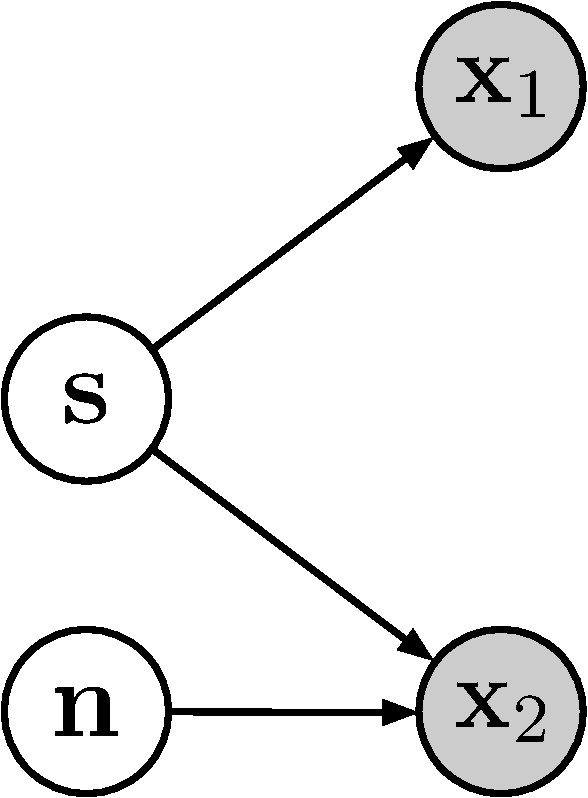
\includegraphics[scale=0.3]{img_pdf/one_noisy.pdf}
	\caption{The setting considered in Section \ref{sec:onenoisless}. Two views of the sources are available, one of which, $X_1$, is not corrupted by noise. In this and all subsequent figures in this chapter, each node is a deterministic function of its parents in the graph.
	}
	\label{fig:generalized_hsr_basic}
\end{figure}

\medskip

\begin{theorem}
	\label{thm:noiseless1}
	The difference between the log joint probability and log product of marginals of the observed variables in the model given in Equations \ref{eq:indep}-\ref{eq:sem2_1} admits the following factorisation:
	\begin{align}
	&\log p({x}_1, {x}_2) - \log p({x}_1) p({x}_2) \nonumber \\
	&= \log p({x}_2 | {x}_1) - \log p({x}_2) \nonumber\\
	&= \left(\sum_i \alpha_i(z_{i}, g_i(z_i, n_i)) + \log \det J \right) \nonumber\\
	&\qquad - \left( \sum_i \delta_i(g_i(z_i, n_i)) + \log \det J\right) \nonumber\\
	&= \sum_i \alpha_i(z_{i}, g_i(z_i, n_i)) - \sum_i \delta_i(g_i(z_i, n_i))\label{eq:logdens_noiesless_1} \,
	\end{align}
	where $z_i=f^{-1}_{1i}({x}_1)$, $g_i=f^{-1}_{2i}({x}_2)$,
	and $J$ is the Jacobian of the transformation $f^{-1}_2$ (note that the introduced Jacobians cancel\footnote{Several subsequent results in this section consider the difference between two log-probabilities.
In all of these cases, the Jacobians introduced by a change of variables cancel out as in Equation \ref{eq:logdens_noiesless_1}.
For brevity these Jacobians are omitted henceforth.}).
	Suppose that
	\begin{enumerate}
		\item $\alpha$ satisfies the \emph{Sufficiently Distinct Views} assumption (see after this theorem).
		\item A classifier is trained to discriminate between
		\begin{align*}
		(X_{1},X_{2}) \text{ vs. } (X_{1},X_{2}^{*})\,,
		\end{align*}
		where $({X}_{1},{X}_{2})$ correspond to the same realisation of $Z$ and $({X}_{1},{X}_{2}^{*})$ correspond to different realisations of ${Z}$.
		\item The classifier minimises the logistic regression loss, and is constrained to use a regression function of the form
		\begin{equation*}
		r({x}_{1},{x}_{2})=\sum_{i}\psi_{i}(h_{i}({x}_{1}),{x}_{2})
		\end{equation*}
		where ${h} =(h_{1}, \ldots, h_{n})$  is invertible, smooth and has smooth inverse.
	\end{enumerate}
	
	Then, in the limit of infinite data and with universal approximation capacity, $h$ inverts ${f}_1$ in the sense that the $h_{i}(X_1)$ recover the independent components of $Z$ up to component-wise invertible transformations.
\end{theorem}
An outline of the proof for this result is provided below after discussing some of the assumptions; full proof can be found in Appendix \ref{appendix:proof-thm1}.

The assumption of invertibility for $h$ could be satisfied by, e.g., the use of normalizing flows~\citep{rezende2015variational, chen2018neural} or deep invertible networks~\citep{jacobsen_hal-01712808}.


If $X_1$ and $X_2$ were always equal, the multiple view setting would reduce to the normal nonlinear ICA setting.
The \emph{Sufficiently Distinct Views (SDV)} assumption formalises a sense in which the two views must be sufficiently different from one another,
resulting in more information being available in totality than from each view individually.
In the context of Theorem~\ref{thm:noiseless1}, it is an assumption about the log-probability of the \emph{corruption} conditioned on the source.
Informally, it demands that the probability distribution of the corruption should vary significantly as a result of conditioning on different values of the source.

\medskip

\begin{definition}[Sufficiently Distinct Views]\label{suff_dist_assumption}
	Let $\alpha_i(y_i, t_i)$, $i=1,\ldots, D$ be functions of two arguments.
	Denote by $\alpha$ the vector of functions and define
	\begin{align}
	\alpha'_{i}(y_i, t_i)&= \partial \alpha_{i}(y_i, t_i)/\partial y_i, \label{eq:convention1}\\
	\alpha''_{i}(y_i, t_i)&=\partial^2 \alpha_{i}(y_i, t_i)/\partial y_i^2\, \label{eq:convention2}\\
	{w}_{\alpha}({y}, {t}) &= (\alpha''_{1}, \ldots, \alpha''_{D}, \alpha'_{1}, \ldots,\alpha'_{D}).
	\end{align}
	We say that ${\alpha}$ satisfies the assumption of \emph{Sufficiently Distinct Views (SDV)} if for any value of ${y}$, there exist $2D$ distinct values ${t}^j$, $j=1, \ldots, 2D$ such that the vectors ${w}({y},{t}^j)$ are linearly independent.
	\\    \end{definition}
This is closely related to the Assumption of Variability in~\cite{hyvarinen19a}.
The SDV assumption is discussed in further detail in Section \ref{appendix:sdv}, where simple cases of conditional log-probability density functions satisfying and violating the assumption are presented.



\begin{proof}[Sketch proof of Theorem \ref{thm:noiseless1}]
The first observation to be made is that for logistic regression, the optimal regression function for the logit $r(x_1, x_2)$ is equal to the log density-ratio between the two distributions being distinguished, namely $\log\left( p(x_1, x_2) / p(x_1)p(x_2)\right) = \log p(x_1, x_2) - \log p(x_1)p(x_2)$.
Thus, in the limit of infinite data and with universal approximation capacity, the following equality holds:
%
\begin{align*}
\sum_{i}\psi_{i}(h_{i}({x}_{1}),{x}_{2}) = \sum_i \alpha_i(z_i, g_i(z_i, n_i)) - \sum_i \delta_i(g_i(z_i, n_i)).
\end{align*}
%
By performing the change of variables $y=h(x_1)$, $t=f_2^{-1}(x_2)$, and defining $v(y) := f_1^{-1}(h^{-1}(y)) = z$, this equation can be rewritten
%
\begin{align}
\sum_{i}\psi_{i}(y_i,f_2(t)) = \sum_i \alpha_i(v_i(y), t_i) - \sum_i \delta_i(t_i). \label{eqn:ica-first-theorem-proof}
\end{align}
%
The goal is to show that $v_i(y)$ depends on exactly one coordinate of $y$, so that $v_i(y) = v_i(y_j)$ for some $j$. 
Since $z = v(y)$, this implies that $z_i = v_i(y_j)$ is a function only of $y_j$, which in turn implies that $z_i$ is a function only of $h_j(x_1)$. 
Since $v = f_1^{-1} \circ h^{-1}$ is the composition of two invertible functions, it is itself invertible, and since each component of $v$ depends only one one component of its input, each of the components are also invertible.
It follows that $z_i$ is an invertible function of $h_j(x_1)$, and so $h(x_1)$ recovers $z$ up to permutations and coordinate-wise invertible transformations.

Showing that $v_i(y) = v_i(y_j)$ for some $j$ is somewhat technically involved, and it is here that the SDV assumption is required.
It is proved by taking partial derivatives of Equation \ref{eqn:ica-first-theorem-proof} with respect to $y_i$ and $y_j$ for $j\not=i$. 
This results in an expression involving first- and second-order derivatives of $\alpha_i$ and $v_i$ in which the expressions in the SDV assumption appear. 
If the SDV assumption holds, it follows that the derivative of $v_i$ with respect to $y_j$ is everywhere zero, meaning that $v_i$ does not depend on $y_j$. 
\end{proof}

See the full proof in Appendix \ref{appendix:proof-thm1} for further details; proofs of subsequent results Corollary \ref{crl:noiseless1} and Theorems \ref{thm:demixing} and \ref{thm:two-noisy-views} proceed similarly to this, and thus sketches of these results will be omitted.

Theorem \ref{thm:noiseless1} shows that by jointly considering the two views, it is possible to recover $Z$, in contrast to the single-view setting.
This result can be extended to learn the inverse of ${f}_2$ up to component-wise invertible functions.

\medskip

\begin{corollary}
	\label{crl:noiseless1}
	Consider the setting of Theorem \ref{thm:noiseless1} with the alternative factorisation of the log joint probability
	\begin{align}
	&\log p({x}_1, {x}_2) - \log p({x}_1) p({x}_2) \nonumber \\
	&= \log p({x}_1 | {x}_2) - \log p({x}_1)\nonumber \\
	&= \sum_i \gamma_i(z_i, g_i(z_i, n_i)) - \sum_i \beta_i(z_i)) \label{eq:logdens_noiesless_2}\,.
	\end{align}
	Suppose that ${\gamma}$ satisfies the SDV assumption.
	Replacing the regression function with
	\begin{equation*}
	r({x}_{1},{x}_{2})=\sum_{i}\psi_{i}({x}_{1}, h_{i}({x}_{2}))
	\end{equation*}
	results in ${h}$ inverting ${f}_2$ in the sense that the $h_{i}({X}_2)$ recover the independent components of the ${g}({Z}, {N})$ up  to component-wise invertible transformations.
\end{corollary}
The proof can be found in Appendix \ref{appendix:proof-cor2}.
Theorem \ref{thm:noiseless1} and Corollary \ref{crl:noiseless1} together mean that it is possible to learn inverses ${h}_1$ and ${h}_2$ of ${f}_1$ and ${f}_2$, and therefore to recover ${Z}$ and ${g}({Z}, {N})$, up to component-wise intertible functions.
Note, however, that doing so requires running two separate algorithms.
Furthermore, there is no guarantee that the learned inverses ${h}_1$ and ${h}_2$ are `aligned' in the sense that for each $i$ the components ${h}_{1i}({X}_1)$ and ${h}_{2i}({X}_2)$ correspond to the same components of ${Z}$.

This problem of misalignment can be resolved by changing the form of the regression function.

\medskip

\begin{theorem}\label{thm:demixing}
	Consider the settings of Theorem \ref{thm:noiseless1} and Corollary \ref{crl:noiseless1}.
	Suppose that both ${\alpha}$ and ${\gamma}$ satisfy the SDV assumption.
	Replacing the regression function with
	\begin{equation}\label{eqn:double-regression-fn}
	r({x}_{1},{x}_{2})=\sum_{i}\psi_{i}(h_{1,i}({x}_{1}),h_{2,i}({x}_{2}))
	\end{equation}
	results in ${h}_1$, ${h}_2$ inverting ${f}_1$, ${f}_2$ in the sense that the $h_{1,i}({X}_1)$ and $h_{2,i}({X}_2)$ recover the independent components of ${Z}$ and ${g}({Z}, {N})$ up to two different component-wise invertible transformations. Furthermore, the two representations are aligned, i.e. for $i\not=j$,
	\begin{equation*}
	h_{1,i}({X}_{1})\independent h_{2,j}({X}_{2}).
	\end{equation*}
\end{theorem}
The proof can be found in Appendix \ref{appendix:thm1}.
Note that Theorem \ref{thm:demixing} is \emph{not} a generalisation of Theorem \ref{thm:noiseless1} or Corollary \ref{crl:noiseless1}, since it makes stricter assumptions by imposing the SDV assumption on both ${\alpha}$ and ${\gamma}$.
In contrast, Theorem \ref{thm:noiseless1} and Corollary \ref{crl:noiseless1} require that only one is valid for each.
For cases in which finding aligned representations for ${Z}$ and ${g}({Z}, {N})$ are desired, Theorem \ref{thm:demixing} should be applied.
If the only goal is recovery of ${Z}$, the assumptions of Theorem \ref{thm:noiseless1} are easier to satisfy.


In practical applications, the multi-view scenario is useful in multimodal datasets where one of the two acquisition modalities has much higher signal to noise ratio than the other one (e.g., in neuroimaging, when simultaneous fMRI and Optical Imaging recordings are compared). In such cases,
these results show that jointly exploiting the multiple modalities can lead to identification of the true underlying sources in a manner not attainable through use of the more reliable modality alone.

%would help to discern a meaningful and identifiable latent representation which could not be attained through analysis of the more reliable modality alone.


%\subsubsection{Equivalence with Permutation Contrastive Learning for Time Dependent Sources}
%Note that the analysis of Theorem~\ref{thm:noiseless1} covers the case of temporally dependent stationary sources analyzed in~\cite{pmlr-v54-hyvarinen17a}.
%Indeed, if it is further assumed that $\bm{s}$ and $\bm{g}(\bm{s}, \bm{n})$ are uniformly dependent~\cite{pmlr-v54-hyvarinen17a}, they can be seen as a pair of subsequent time points of an ergodic stationary stochastic process for which the analysis of Theorem 1 of~\cite{pmlr-v54-hyvarinen17a} would hold. In other words, we can define a stochastic process as $p(\bm{s}_{t+1}| \bm{s}_t) := p(\bm{g}(\bm{s}, \bm{n})| \bm{s})$.
%Note that while the two formulations are theoretically equivalent, our view offers a wider applicability as it covers the asynchronous sensing of $\bm{s}$, provided that multiple measurements (i.e. $\bm{x}_1, \bm{x}_2$) are available; additionally, our \textit{Sufficiently Distinct Views} assumption does not necessarily imply uniform dependency. Furthermore, while~\cite{pmlr-v54-hyvarinen17a} considers a generative model of the form $\bm{x}(t) = \bm{f}(\bm{s}(t))$, thus constraining the mixing function to be the same for any two data points $\bm{x}(t_1)$, $\bm{x}(t_2)$, in our setting we consider two different mixing functions, $\bm{f}_1$ and $\bm{f}_2$, for the two different views.
%Finally, we study this setting as an intermediate step for the following two sections, in which no deterministic function of the sources is observed, learning to invert any of the $\bm{f}_i$ can only recover $\bm{s}$ up to the corruption operated by $\bm{g}$.

\subsection{Two noisy views}
\label{sec:constrained}

\begin{figure}[t!]
	\centering
		\begin{tikzpicture}
		\node[icavar] (Z) at(0,0) {$Z$};
		\node[icavar] (N1) at(0,1.5) {$N_1$};
		\node[icavar] (N2) at(0,-1.5) {$N_2$};
		\node[icavarobs] (X2) at(2,-1.5) {$X_2$};
		\node[icavarobs] (X1) at(2,1.5) {$X_1$};
		\draw[->] (Z) -- (X1);
		\draw[->] (Z) -- (X2);
		\draw[->] (N2) -- (X2);
		\draw[->] (N1) -- (X1);
		\end{tikzpicture}
%	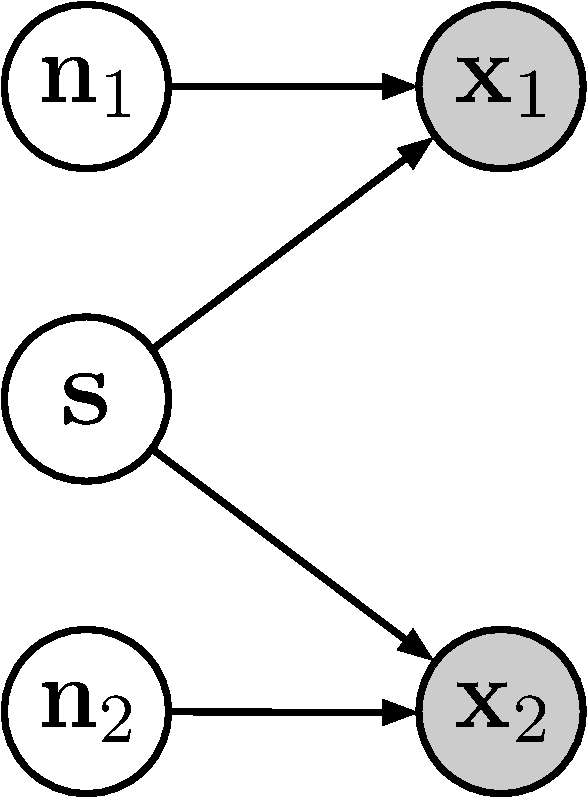
\includegraphics[scale=0.3]{img_pdf/classic_hsr.pdf}
	\caption{Setting with two views of the sources $Z$, both corrupted by noise.}
	\label{fig:classic_hsr}
\end{figure}

Consider next the setting in which both variables are corrupted by noise, depicted in Figure \ref{fig:classic_hsr} and described by the following model:
\begin{align*}
X_{1}&={f}_{1}({g}_{1}({Z},N_{1}))  \\
X_{2}&={f}_{2}({g}_{2}({Z},N_{2}))  \,,
\end{align*}
where all variables take value in $\mathbb{R}^D$, ${f}_{1}$ and ${f}_{2}$ are nonlinear, invertible, deterministic functions,
${g}_{1}$ and ${g}_{2}$ are component-wise corrupters, and $Z$ and the $N_i$ are independent with independent components.
This class of models generalises the setting of Section \ref{sec:onenoisless}, since by taking ${g}_1(Z, N_1) = Z$ it reduces to the case of one noiseless observation.

The log density-ratio $\log p({x}_1, {x}_2) - \log p({x}_1)p({x}_2)$ admits similar factorisations to those given in Equations \ref{eq:logdens_noiesless_1} and \ref{eq:logdens_noiesless_2}:
\begin{align}
&\log p({x}_1, {x}_2) - \log p({x}_1) p({x}_2) \nonumber\\
&= \log p({x}_1 | {x}_2) - \log p({x}_1)\nonumber\\
&= \sum_i \eta_i(g_{1i}(z_i, n_{i1}), g_{2i}(z_i, n_{2i})) - \sum_i \theta_i(g_{1i}(z_i, n_{1i}) \label{eq:noisylogdens_1}\\
&= \log p({x}_2 | {x}_1) - \log p({x}_2) \nonumber\\
&= \sum_i \lambda_i(g_{2i}(z_i, n_{2i}), g_{1i}(z_i, n_{1i})) - \sum_i \mu_i(g_{2i}(z_i, n_{2i})) \label{eq:noisylogdens_2}
\end{align}
Since access is only given to corrupted observations, exact recovery of $Z$ is not possible.
Nonetheless, a generalisation of Theorem \ref{thm:demixing} holds showing that the ${f}_i$ can be inverted and $Z$ recovered up to the corruptions induced by the $N_i$ via the ${g}_i$.

\medskip

\begin{theorem}\label{thm:two-noisy-views}
	Suppose that ${\eta}$ and ${\lambda}$ satisfy the SDV assumption.
	The algorithm described in Theorem \ref{thm:noiseless1} with regression function specified in Equation \ref{eqn:double-regression-fn} results in ${h}_1$ and ${h}_2$ inverting ${f}_1$ and ${f}_2$ in the sense that the $h_{1,i}({X}_1)$ and $h_{2,i}({X}_2)$ recover the independent components of ${g}_1({Z}, {N}_1)$ and ${g}_2({Z}, {N}_2)$ up to two different component-wise invertible transformations. Furthermore, the two representations are aligned, i.e. for $i\not=j$,
	\begin{equation*}
	h_{1,i}({X}_{1})\independent h_{2,j}({X}_{2}).
	\end{equation*}
\end{theorem}
The proof can be found in Appendix \ref{appendix:thm1}.

We can thus recover the common source $Z$ up to the corruptions ${g}_i(Z, N_i)$.
In the limit of the magnitude of one of the noise variables going to zero, the reconstruction of the sources $Z$ attained through the corresponding view is exact up to the component-wise invertible functions, as stated in the following corollary.

\medskip
\begin{corollary}
	\label{crl:lownoise}
	Let $N_1^{(k)} = \frac{1}{k} \cdot  \Tilde{N}$ for $k \in \NN$, where $\Tilde{N}\in\mathbb{R}^D$ is a fixed random variable with finite variance, and let $N_2$ be a random variable that does not depend on $k$.
	Let $h_1^{(k)}, h_2^{(k)}$ be the output of the algorithm specified by Theorem \ref{thm:two-noisy-views} with noise variables $N_1^{(k)}$ and $N_2$.
	
	Suppose that the corrupters $g_i$ satisfy the following two criteria:
	\begin{enumerate}
		\item $\exists {a}  \in \mathbb{R}_{> 0}^D \: $   s.t. $\: \left|\frac{\partial g_1(z,n)}{\partial n} \right|_{n=0} \leq {a} \: $ for all ${z}$
		\item $\exists {b}  \in \mathbb{R}_{> 0}^D \: $ s.t. $\: 0<\frac{\partial g_1(z,0)}{\partial z} \leq b$
	\end{enumerate}
	Then, denoting by $\mathcal{E}$ the set of all component-wise, invertible functions, it holds that
	\[
	 \inf_{{e}\in \mathcal{E}}  \left \|Z - {e}(h_1^{(k)}(X_1)) \right \| \xrightarrow[k \to \infty]{p} 0
	\]
	where $p$ denotes convergence in probability.
\end{corollary}

\begin{proof}[Sketch; see Appendix \ref{appendix:thm2} for full proof.]
The key idea of the proof is to rewrite ${e}(h_1^{(k)}(X_1))$ as $\tilde{e} \circ g_1(Z, N_1^{(k)})$ for some $\tilde{e} \in \mathcal{E}$, and to Taylor expand $g_1(Z, N_1^{(k)})$ in its second argument.
Together with the assumptions on $g_1$, it is proved that the random variable converges to $0$ in mean, which implies that it converges to $0$ in probability.
\end{proof}

%\begin{corollary}
%	Let $\bm{n}_1^{(k)} = \frac{1}{k} \cdot  \Tilde{\bm{n}}$ for $k \in \NN$, where $\Tilde{\bm{n}}\in\mathbb{R}^D$ is a fixed random variable, and $\bm{n}_2$ be a random variable that does not depend on $k$.
%	Let $\bm{h}_1^{(k)}, \bm{h}_2^{(k)}$ be the output of the algorithm specified by Theorem \ref{thm:two-noisy-views} with noise variables $\bm{n}_1^{(k)}$ and $\bm{n}_2$.
%	
%	Suppose that the corrupters $\bm{g}_i$ satisfy the following two criteria:
%	\begin{enumerate}
%		\item $\exists \bm{a}  \in \mathbb{R}_{> 0}^D \: $   s.t. $\: \left|\frac{\partial \bm{g}_1(\bm{s},\bm{n})}{\partial \bm{n}} \right|_{\bm{n}=0} \leq \bm{a} \: $ for all $\bm{s}$
%		\item $\exists \bm{b}  \in \mathbb{R}_{> 0}^D \: $ s.t. $\: 0<\frac{\partial \bm{g}_1(\bm{s},0)}{\partial \bm{s}} \leq \bm{b}$
%	\end{enumerate}
%	Then, denoting by $\bm{E}$ the set of all scalar, invertible functions, we have that
%	\[
%	\lim_{k \to \infty} \inf_{\bm{e}\in \bm{E}} \left \|\bm{s} - \bm{e}(\bm{h}_1^{(k)}(\bm{x}_1)) \right \| = 0
%	\]
%\end{corollary}

Corollary \ref{crl:lownoise} implies that in the limit of small noise, the sources $Z$ can be recovered exactly.
Condition $1$ upper bounds the influence of $N_1$ on the corruption: one cannot not hope to recover $Z$ if $g_1(Z, N_1)$ contains too little signal.
Condition $2$ ensures that the function $g_1$ is invertible with respect to $z$ when $n_1$ is equal to zero.
If this were not satisfied, some information about $Z$ would be washed out by $g_1$ even in absence of noise, which would make recovery of $Z$ trivially impossible.
These conditions are satisfied, for example, by additive noise.


\subsection{Multiple noisy views}
\label{sec:multiple}

The results of Section \ref{sec:constrained} state that in the two noisy views setting, $Z$ can be recovered up to the corruptions.
In the limit that the magnitude of the noises goes to zero, the uncorrupted $Z$ can be recovered.
The intuition is that the less noise there is, the more information each observation provides about $Z$.

\begin{figure}[t!]
	\centering
		\begin{tikzpicture}
		\node[icavar] (Z) at(0,0) {$Z$};
		\node[icavar] (Ni) at(0,1.7) {$N_i$};
		\node[icavarobs] (Xi) at(3,1.7) {$X_i$};
		\draw[->] (Z) -- (Xi);
		\draw[->] (Ni) -- (Xi);
		\draw[solid] (-.75,2.45) -- (3.75,2.45) -- (3.75,.85) -- (-.75,.85) -- (-.75,2.45);
		\node[](text) at(0.5,1.05) {\scriptsize $i=1,\ldots,M$};
		\end{tikzpicture}	
%	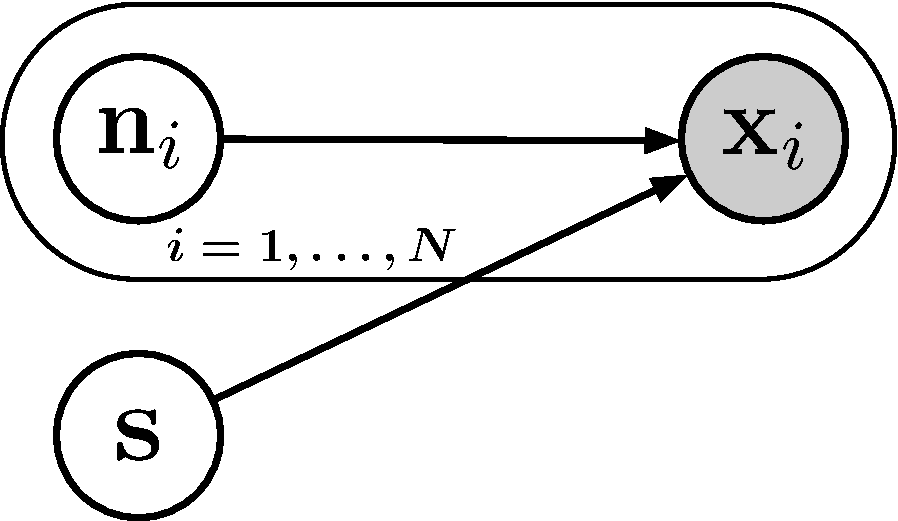
\includegraphics[scale=0.3]{img_pdf/generalized_hsr_many.pdf}
	\caption{The setting of Section \ref{sec:multiple} with $M$ corrupted views of the sources.}
	\label{fig:generalized_hsr_many}
\end{figure}

This section considers the multi-view setting, where $M$ distinct noisy views of $Z$ are available,
\begin{equation*}
X_{i}={f}_{i}({g}_{i}(Z,N_{i})),\,\,\,i=1, \ldots, M\,, \label{eq:multi}\\
\end{equation*}
and the noise variables $N_{i}$ are mutually independent, as represented in Figure \ref{fig:generalized_hsr_many}.
Since each view provides additional information about $Z$, the question naturally arises: in the limit as $M \to \infty$, is it possible to reconstruct $Z$ exactly?


By applying Theorem \ref{thm:two-noisy-views} to the pair $({X}_1,X_i)$ it is possible to recover  $({g}_1(Z,N_1),{g}_i(Z,N_i))$ such that the components are aligned, but up to different component-wise invertible functions ${k}_1$ and ${k}_i$.
Running the algorithm on a different pair  $({X}_1,X_{j})$ will result in recovery up to different component-wise invertible functions $k'_1$ and $k'_j$.

Note that these will \emph{not} necessarily result in  ${k}_i\circ{g}_i(Z,N_i)$ and ${k}'_j\circ{g}_j(Z,N_j)$ being aligned with each other.
However, the components of ${k}_1\circ{g}_1(Z,N_1)$ and ${k}'_1\circ{g}_1(Z,N_1)$ are the same, up to permutation and component-wise invertible functions.
This permutation can therefore be undone by performing independence testing between each pair of components.
Components that are `different' will be independent; those that are the same will be deterministically related.
Therefore, they can be used as a reference to permute the components of ${k}'_j$ and make it aligned with ${k}_i$.

The problem is then how to combine the information from each aligned ${k}_i \circ {g}_i(Z,N_i)$ to more precisely identify $Z$.
The fact that the components are recovered up to \emph{different} scalar invertible functions makes combining information from different views non-trivial.


As a first step in this direction, consider the special case that each ${g}_i$ acts additively and each $N_i$ is zero mean and each of $Z$ and the $N_i$ are independent with independent components.
\begin{align}
\left.
\begin{array}{ll}
&X_{i}={f}_{i}(Z + N_{i}) \\
&\mathbb{E}[N_i]= 0
\end{array}
\right\rbrace \quad i \in \mathbb{N}
\end{align}

Suppose to begin with that it is possible to recover each $Z + N_i$ \emph{without} the usual component-wise invertible functions. Then, writing $N$ to denote all of the $N_i$, it is possible to estimate $Z$ as
\begin{align*}
Z \approx \Omega^M(Z, N) = \frac{1}{M}\sum_{i=1}^M \left(Z + N_i\right).
\end{align*}
Subject to mild conditions on the rate of growth of the variances $\text{Var}(N_i)$ as $i\to\infty$, Kolmogorov's strong law implies that $\Omega^M(Z, N)$ is a good approximation to $Z$ as $M\to\infty$ in the sense that  $\Omega^M(Z, N) \overset{a.s.}{\longrightarrow} Z$.
This implies moreover that it is possible to reconstruct the $N_i$ by considering the residue $R^N_i(Z, N) = (Z + N_i) - \Omega^M(Z, N) \overset{a.s.}{\longrightarrow} N_i$.

In the presence of the unknown functions ${k}_i$, we would be able to reconstruct $Z$ and the $N_i$ if we were able to identify the inverses ${e}_i = {k}_i^{-1}$ for each $i$.
For any component-wise invertible functions ${e}_i$, define
\begin{align*}
\Omega_{e}^M(Z, N) &= \frac{1}{M} \sum_{i=1}^M {e}_i\circ {k}_i( Z + N_i) \\
R_{{e}, i}^M(Z, N) &= {e}_i\circ {k}_i( Z + N_i) - \Omega_{{e}}^M(Z, N).\\
\end{align*}
${e}_i$ is something we can choose and ${k}_i(Z+N_i) = {h}_i({X}_i)$ is the output of the algorithm, and hence $\Omega_{e}^M(Z, N)$ and $R_{{e}, i}^M(Z, N)$ are random variables with known distributions.
Subject to mild conditions, the dependence of these quantities on most or all of the $N_i$ becomes increasingly small as $M$ grows and disappears in the limit $M\to\infty$.

\medskip

\begin{lemma}\label{lem:last-lemma}
	Suppose that the sequence $\mathbb{E}_{N}[\Omega_{e}^M(Z, N)] = \frac{1}{M}\sum_{i=1}^M \mathbb{E}_{N_i}[{e}_i\circ {k}_i( Z + N_i)] $ converges as $M \to \infty$ for almost all $Z$, and write this limit as
	\begin{align*}
	\Omega_e(Z) = \lim_{M\to\infty}\mathbb{E}_{N}[\Omega_{e}^M(Z, N)].
	\end{align*}
	
	Suppose further that there exists $K$ such that $V_{e_i} = \mathrm{Var}\left({e}_i \circ {k}_i(Z + N_i) \right) \leq K$ for all $i$.
	Then
	\begin{align*}
	\Omega_{e}^M(Z, N) & \overset{a.s.}{\longrightarrow} \Omega_{e}(Z) \\
	R_{e, i}^M(Z, N) & \overset{a.s.}{\longrightarrow} R_{e, i}(Z, N_i) = {e}_i\circ {k}_i( Z + N_i) - \Omega_{e}(Z)
	\end{align*}
\end{lemma}
\begin{proof}[Sketch; see Appendix \ref{appendix:last-lemma} for full proof]
The result follows by applying Kolmogorov's strong law to $\Omega_{e}^M(Z, N)$ for each value of $Z$.
Kolmogorov's strong law states that the average of a sequence of independent, but not necessarily identically distributed, random variables converges to the expectation of the average, provided that the variances of the random variables do not grow too quickly. 
This is ensured by the assumption on the $V_{e_i}$.
\end{proof}

%The proof can be found in Appendix \ref{appendix:last-lemma}. \todo{give sketch}

Given some choice of ${e}$, the quantities $\Omega_{e}(Z)$ and $R_{e, i}(Z, N_i)$ can be thought of as putative candidates for $Z$ and $N_i$ respectively.
As discussed earlier, if it were possible to identify ${e}_i={k}_i^{-1}$, then it would be the case that $\Omega_{e}(Z) = Z$ and $R_{e, i}(Z, N_i) = N_i$, and thus $\Omega_{e}$ and $R_{e, i}$ would satisfy the same independences and other statistical properties as $Z$ and $N_i$ respectively.
Can these properties be used as criteria to identify good choices of ${e}_i$?

The following theorem provides sufficient conditions which, if satisfied by a putative choice for the $e_i$, implies that they invert the $k_i$ up to some affine ambiguity for all $i$. 

%The following theorem gives a set of sufficient conditions under which each ${e}_i$ inverts ${k}_i$ up to some affine ambiguity which is the same for every $i$.
%Under these conditions, the properties discussed in the previous paragraph are sufficient to identify whether a putative choice for $e$ indeed results in recovery of the sources.

\medskip

\begin{theorem}
	\label{thm:lastthm}
	Suppose there exists $C>0$ such that $\text{Var}(N_i) \leq C$ for all $i$ and let $\mathcal{G}_K = \big\lbrace
	\{{e}_i \}$ s.t.
	\begin{align}
	& V_{{e}_i} \leq K \ \forall i \label{eq:resid_1}\\
	& \Omega_{{e}}(Z) < \infty \  \text{ for almost all } Z \label{eq:resid_2}\\
	&R_{{e}, i} \independent R_{{e}, j} \ \forall i \not= j, \label{eq:resid_3}\\
	\nonumber \\    &\mathbb{E} R_{{e}, i} = 0 \ \forall i \label{eq:resid_5} \\
	&R_{{e}, i}(Z, N_i) = R_{{e}, i}(N_i) \ \forall i \ \big\rbrace \label{eq:resid_6}
	\end{align}
	
	Then,
	\begin{align*}
	\mathcal{G}_K \subseteq\left\lbrace \{ {\alpha} {k}^{-1}_i + {\beta} \} \ : \ {\alpha} \in \mathbb{R}^{D}_{\not=0}, \: {\beta} \in \mathbb{R}^{D} \right\rbrace
	\end{align*}
	where $\alpha {k}^{-1}_i$ denotes the element-wise product with the scalar elements of ${\alpha}$.
	If $K \geq \text{Var}(Z) + C$, then $ \{ {k}^{-1}_i \}  \in \mathcal{G}_K$,
	and so $\mathcal{G}_K$ is non-empty for $K$ sufficiently large.
\end{theorem}
\begin{proof}[Sketch; see Appendix \ref{sec:lasttmpr} for full proof]
That $\{ {k}^{-1}_i \}  \in \mathcal{G}_K$ can be shown using Lemma \ref{lem:last-lemma}. 
The fact that $\mathcal{G}_K \subseteq\left\lbrace \{ {\alpha} {k}^{-1}_i + {\beta} \} \ : \ {\alpha} \in \mathbb{R}^{D}_{\not=0}, \: {\beta} \in \mathbb{R}^{D} \right\rbrace$ is proved by showing that for any $e_i$ such that $\{e_i\} \in \mathcal{G}_K$, the composition $e_i \circ k_i$ is affine.
It follows that $e_i = A_i k_i^{-1} + \beta_i$ for some matrix $A_i$ and vector $\beta_i$. 
Finally, it is shown that $A_i$ and $\beta_i$ are equal for all choices of $i$, and $A$ is a diagonal matrix, and thus $A k_i^{-1}$ can be written as an elementwise product with a vector $\alpha$.
\end{proof}

It follows that it is possible recover $Z$ and $N_i$ up to ${\alpha}$ and ${\beta}$ via $\Omega_e(Z) = {\alpha}Z + {\beta}$ and $R_{{e}, i}(N_i) = {\alpha}N_i$.

Each of the conditions \ref{eq:resid_1}--\ref{eq:resid_5} can be verified from known information.
We conjecture that condition \ref{eq:resid_6} can be relaxed to assuming the verifiable condition of independence between $\Omega_{e}(Z)$ and $R_{e, i}(Z, N_i)$ for all $i$ along with additional regularity assumptions on the functional form of $R_{e, i}$ (e.g. smoothness).

To conclude, Theorem \ref{thm:lastthm} provides sufficient conditions under which it is possible to fully reconstruct $Z$ with corrupted views.
In contrast to previous results in Sections \ref{sec:onenoisless} and \ref{sec:constrained}, this result leverages infinitely many corrupted views rather than vanishingly small corruption of finitely many views.




\section{Discussion about assumptions}\label{sec:ica-assumptions}

This section discusses in further detail the Sufficiently Distinct Views (SDV) assumption and the necessity for source-level noise for at least one of the views.

Typically, noise is a nuisance variable that would preferably not exist.
In the setting considered here however, the presence of some source-level noise is necessary, since without this the classification based approach cannot be applied.
Furthermore, the SDV assumption is ultimately an assumption about how the corrupted sources corresponding to each view are related, and is by implication an assumption about the source corruptions themselves.



\subsection{The Sufficiently Distinct Views assumption}
\label{appendix:sdv}

Recall that the SDV assumption is a demand on how much the conditional probability distribution of the source of one view given another varies, e.g. how much $p(z_1 | z_2)$ changes as a function of $z_2$ where $z_i = f_1^{-i}(x_i)$. 
To provide intuition, this section gives examples of cases in which the SDV assumption does and does not hold.

The SDV assumption is closely related to the \emph{Assumption of Variability} of \cite{hyvarinen19a}, an analogous assumption that occurs in the context a different graphical model from the multi-view setting considered here; see that paper for further details.




%We give the following two examples to provide intuition about the Sufficiently Distinct Views (SDV) assumption - one regarding a case in which it does not hold, and another one in which it does.

\subsubsection{An example violating SDV}

Suppose that the conditional distribution of one corrupted source given the other is Gaussian, so that

\begin{equation}
\log p(z_1|z_2) =  -\sum_i (z_{1i} - z_{2i})^2/(2\sigma_i^2) + C \,, \label{eq:unsatisfied}
\end{equation}

where $C$ is a constant.
Since taking second derivatives of the log-probability with respect to $s_i$ results in constants,
there is no way to find $2D$ vectors ${t}_j$, $j=1, \ldots, 2D$, such that the corresponding ${w}(z_1, t_j)$ in Definition \ref{suff_dist_assumption} are linearly independent.

This rules out the case in which one or both views correspond to the source being corrupted by additive Gaussian noise.

Note that this result is distinct from the non-identifiability result in the case of Gaussian sources for ICA.
The problem here is not that the conditional distribution is rotationally invariant, but that the connection it implies between the two variables is `too simple'.
In fact, the identifiability results presented here do not demand that the marginal distribution over the uncorrupted source be non-Gaussian.

%The fact that the assumption breaks down in this case is reminiscent of the breakdown in the case of Gaussianity for linear ICA. Interestingly, in our work, the true latent sources \textbf{are} allowed to be Gaussian. In fact, the distribution of $\bm{s}$ does not enter the expression above.


\subsubsection{An example satisfying SDV}

By choosing a conditional distribution  that is more comlex, the SDV assumption can be satisfied. Consider

\begin{equation}
\log p(z_1|z_2) =  - \sum_i (z_i^2  s_i^2 + z_i^4 s_i^4  ) + C(z_2) \,, \label{eq:satisfied}
\end{equation}

where $C(z_2)$ is a normalisation constant that depends only on $z_2$.
Proof that this conditional distribution satisfies the SDV assumption requires a few lines of computation.

Since this polynomial expression is of order strictly greater than 2, the second derivatives are not constant.
${w}(z_1, z_2)$ can be written as the product of a matrix and vector which are functions only of $z_1$ and $z_2$ respectively.
The columns of this matrix are linearly independent for almost all values of $z_1$ and $2D$ linearly independent vectors can be realised by different choices of $z_2$, and hence the assumption is satisfied.


\subsection{Source noise}\label{sec:converged}

Noise on the sources is required for at least one of the views. 
This is a consequence of training a classifier as a way retrieve the the unmixed signals.
The reasons for this are explained briefly here.\footnote{\todo{Rewrite if density ratio estimation is covered in the literature review}}


Suppose that a variable $X$ is drawn with equal probability from two distributions $P_0$ and $P_1$ with densities $p_0(x)$ and $p_1(x)$ respectively.
A classifier $D: x \mapsto [0,1]$ is trained to estimate the posterior probability that a particular realisation of $X$ was drawn from $P_0$ with the cross entropy loss, i.e. the parameters of $D$ are chosen to minimise

\[
L(D) = \mathbb{E}_{X\sim P_0} \left[ - \log D(X) \right] + \mathbb{E}_{X\sim P_1} \left[ - \log (1 - D(X)) \right].
\]

As shown in, for instance, \cite{goodfellow2014generative}, the global optimum of this loss occurs when $D(x) = \frac{p_0(x)}{p_0(x) + p_1(x)}$, which can be rewritten as

\begin{align}
D(x) &= \frac{1}{1 + p_1(x)/p_0(x)}\\
&= \frac{1}{1 + \exp ( - \log (p_0(x)/p_1(x))) } \label{eq:density-ratio-classification}
\end{align}

Recall that in the setting considered in this work, the function $r(x_1, x_2)$ is trained to classify between the two cases that $(x_1, x_2)$ is drawn from the joint distribution $p(x_1, x_2)$ (\emph{class $0$}) or the product of marginals $p(x_1) p(x_2)$ (\emph{class $1$}).
$r(x_1, x_2)$ is trained so that $\frac{1}{1 + \exp(-r(x_1, x_2))}$ estimates the posterior probability of $(x_1, x_2)$ belonging to class 0.
By comparing to Equation \ref{eq:density-ratio-classification}, it can be seen that
%
\begin{align*}
r(x_1, x_2) &= \log \left( p(x_1, x_2) / p(x_1) p(x_2)\right) \\
&= \log p(x_1 | x_2)  - \log p(x_1) \\
&= \log p(x_2 | x_1)  - \log p(x_2) \\
\end{align*}
%
If the variables $x_1$ and $x_2$ are deterministically related, this log-ratio is everywhere either $0$ or $\infty$.
%In order for the classification trick of contrastive learning to be useful, the variables $x_1$ and $x_2$ cannot be deterministically related.
%If this is the case, the log-ratio is everywhere either $0$ or $\infty$ and hence the learned features are not useful.
To see why this is the case, suppose that $x_1$, and $x_2$ are each $N$-dimensional vectors.
If they are deterministically related, $p(x_1, x_2)$ puts mass on an $N$-dimensional submanifold of a $2N$-dimensional space.
On the other hand, $p(x_1)p(x_2)$ will put mass on a $2N$-dimensional manifold since it is the product of two distributions each of which are N-dimensional.

In this case, the distributions $p(x_1, x_2)$ and $p(x_1)p(x_2)$ are therefore not absolutely continuous with respect to one another and thus the log-ratio is ill-defined: $p(x_1, x_2)/p(x_1)p(x_2) = \infty$ at any point $(x_1,x_2)$ at which $p(x_1, x_2)$ puts mass and zero at points where $p(x_1)p(x_2)$ puts mass and $p(x_1,x_2)$ does not.

It follows that the method of classification used in the results considered in this chapter can only be applied when the different views $X_1$ and $X_2$ are not deterministically related.
For this technical reason, the corruptions are necessary.



\section{Conclusion}
\label{sec:on_suffistv}

The main contribution of this chapter was to present identifiability results in a novel multi-view nonlinear ICA setting.
These results are an important contribution to the field since they extend the scarce literature on identifiability results for nonlinear ICA models.


Theorems \ref{thm:noiseless1} and \ref{thm:demixing} state that in contrast to the single-view setting, the two-view setting is identifiable when the mixing functions are arbitrary smooth, invertible nonlinear functions with smooth inverse, provided that one of the views is corrupted at the source level by sufficiently `complex' noise so that the Sufficiently Distinct Views assumption is satisfied. 

Identifiability results are also obtained in the case of corruptions on both views. Theorem \ref{thm:two-noisy-views} states that the sources can be recovered up to the corruptions, and Corollary \ref{crl:lownoise} demonstrates that in limit as one of the corruptions becomes small, the uncorrupted sources can be recovered.

Finally, initial results are presented in Theorem \ref{thm:lastthm} providing conditions under which the uncorrupted sources are identifiable when a large number of views are available, even if these views are all corrupted by source noise.


%We presented identifiability results in a novel setting by extending the formalism of nonlinear ICA.
%We have investigated different scenarios of multi-view latent variable models and provided theoretical proofs on the possibility of inverting the mixing function and recovering the sources in each case.
%Our results thus extend the scarce literature on identifiability for nonlinear ICA models.

%In the classical noiseless ICA setting, the deterministic relationship between the sources and observations means that inverting the mixing function and recovering the sources are equivalent.
%In contrast, we consider views of corrupted versions of the common sources, resulting in the decoupling of the demixing and retrieval of the sources.
%Remarkably, Theorem \ref{thm:lastthm} points towards the possibility of simultaneously solving the two problems in the limit of infinitely many views.
%
%Classical nonlinear ICA is provably non-identifiable because a single view is not sufficiently informative to resolve non-trivial ambiguities when recovering the sources.
%While many papers in the ICA literature have explored placing restrictions either on the source distribution or on the form of the mixing to resolve these ambiguities, in this paper we consider exploiting additional views to constrain the inverse problem.
%Clearly, if a second view is identical to the first, then nothing is gained by its observation.
%Hence, in order for the second view to assist in resolving ambiguity, it must be sufficiently different from the first.
%This is the intuition behind the technical assumption of \emph{sufficiently distinct views}.




The multi-view setting is relevant in a number of real-world applications, namely in all datasets that include multiple distinct measurements of related phenomena.
In practice, it may be better to think of the noise variables rather as intrinsic sources of variability specific to each view.
In most practical applications this would probably not be a significant limitation due to the prevalence of stochasticity in real-world systems.

A specific example application of the work presented here can be found in the field of neuroimaging.
Consider a study involving a cohort of subjects whose response to the presentation of the same stimulus is measured.
One of the key problems in this field is how to extract a shared response from all subjects despite high inter-subject variability and complex nonlinear mappings between latent source and observation~\citep{haxby2011common, chen2015reduced}.
The results presented here provide principled approaches to the extraction and decomposition of the components of the shared response, by considering the measurements to be different views of an underlying shared response that is corrupted by inter-subject variability.


%In particular, the setting described in our model is suited to account for the high variability of the responses throughout the cohort, since the measurement corresponding to each subject is given by a combination of individual variability and shared response.

There are further directions to explore.
Observe that Theorem \ref{thm:lastthm} builds on the setting of Theorem \ref{thm:two-noisy-views}, which only makes use of pairwise information from the observations.
A natural extension of this work would be to investigate algorithms that explicitly make use of $N>2$ views, which may allow relaxation of the additivity assumption on the corruptions.
Furthermore, Theorem \ref{thm:lastthm} provides results that only hold for the asymptotic limit as the number of views becomes large.
Other extensions to this result could include analysis of the case of finitely many views.






%!TEX root = ../thesis.tex
%*******************************************************************************
%****************************** Third Chapter **********************************
%*******************************************************************************
\chapter{Causal Abstractions}

% **************************** Define Graphics Path **************************
\ifpdf
    \graphicspath{{Chapter3/Figs/Raster/}{Chapter3/Figs/PDF/}{Chapter3/Figs/}}
\else
    \graphicspath{{Chapter3/Figs/Vector/}{Chapter3/Figs/}}
\fi

\emph{This chapter is largely based on the paper:}


\begin{quote}
\fullcite{rubenstein2017causal_fullcite}.
\end{quote}

%\citep{rubenstein2017causal}
%\cite{rubenstein2017causal}
%\citet{rubenstein2017causal}

\emph{Sections ... are an in-depth introduction to causality, motivating and explaining the setting considered by the paper.
Sections ... are mostly based on the paper. 
Section ... discusses how this work has influenced the research community and briefly discusses work that builds on it.}



\section{Introduction}

Much of machine learning concerns the statistical relationships between random variables. In this context, the word \emph{statistical} refers to the assumptions that a fixed but unknown probability distribution exists from which observed data are sampled \emph{independently and identically distributed (\iid)}, and that new data at `test time' will similarly be drawn \iid~from this distribution.
Classification is the canonical example of this, where given a set of \iid~samples from a joint distribution $\PP_{XY}$ over input $X$ and discrete target $Y$, the goal is to learn the conditional distribution $\PP_{Y|X}$ giving the probability distribution over targets for each possible input. Other problems such as density estimation can be phrased similarly.
%Given a set of \emph{i.i.d.} samples from a distribution $\PP_X$, the goal of \emph{density estimation} is to learn an approximation to $\PP_X$.

Despite the great empirical successes of machine learning in practical and applied settings in recent years, there remain problems of interest that cannot be cast directly into the framework described above. 
The framework is limited in that it presupposes the existence of a single joint distribution over all of the random variables of interest, with the operations of marginalisation and conditioning then providing the relationships connecting any subset of variables.
But there are many examples of problems for which a single joint distribution over all variables does not suffice. 
For many questions of scientific interest, this is because the problem either implicitly or explicitly concerns an \emph{intervention} or \emph{action} in the world that changes the joint distribution over the observable variables.

For example, we may be interested to understand the influence of diet on longevity, with the aim of improving public health by encouraging people to eat healthily. 
One might find the consumption of expensive imported fruits to be correlated with a longer life. This may well be due to the nutritiousness of such fruits; it could equally well be due to the fact that only wealthy people can afford such a diet, and that such wealth entails better access to medical treatment, sports facilities for exercise and so on. In the former case, intervening in the world by reducing tariffs on imported fruits to make them cheaper and thus encourage their consumption would have a positive effect on public health; in the latter, not.
Similarly, we may observe in the population that taking over-the-counter painkillers is associated with an elevated risk of heart disease. This might be because such painkillers have a negative effect on the cardiovascular system, in which case acting to reduce access to such painkillers might have a positive impact on health outcomes. But if instead the association is because people who have poor health, and thus heightened risk of heart disease, tend to take more painkillers, then such a policy might have little effect other than to increase overall suffering.

These questions are concerned with understanding causal, not statistical, relationships in the world. 
The aim of \emph{causality} is to study causal influence through the lens of a formal mathematical language, in much the same way that statistical machine learning uses the language of probability. 
\emph{Causal inference} or \emph{causal discovery}, a large part of the causality literature, concerns the identification of causal relationships using data.
As the examples above demonstrate, this can be highly non-trivial, with the well-known phrase ``correlation does not imply causation'' standing testament to the simultaneous difficulty and ubiquity of this problem.
Since correlation (or statistical dependence more generally) is a symmetric relation, an asymmetric causal relationship between two variables can never be inferred without other prior knowledge. 
Moreover, simply identifying that two quantities tend to co-occur does not itself imply a causal relation between the two, since both could be causally influenced by a third.

While causal inference is an important problem with a wide variety of applications ranging from astronomy to neuroscience and economics [**citations**], the main contribution of this chapter is to extend and provide greater understanding of \emph{Structural Equation Models (SEMs)}, one of the popular mathematical frameworks for formalising causal relationships between random variables and interventions, along with the variety of probability distributions these entail. 
In particular, this work seeks to understand the implications of modelling causal structure at a different level of \emph{abstraction} compared to the `truth'. For instance, causal influence between variables of interest may be mediated by irrelevant variables that are ignored; interactions between low-level variables may instead be modelled at a macroscopic level, similar to the manner in which temperature and pressure arise as macroscopic properties of a large number of gaseous particles; and though time invariably plays a role in any causal influence in the real world, mathematical models of causal structure may often omit explicit reference to it.
This work additionally sheds new light on \emph{cyclic} SEMs, a previously poorly understood family of causal models, and has implications to existing causal inference algorithms by providing a framework for understanding the limitations of previous approaches.

REWRITE:
The next sections provide a comprehensive background sufficient to understand the novel contribution of this chapter.
In Section ??, we will introduce SEMs, followed in Section ?? by an overview of approaches to causal inference using SEMs. 
In Section ?? we will discuss the implicit assumptions in these approaches to causal inference, which will lead us to discussing causal abstractions in Sections ?? to ??.
Section ?? discusses the influence that this work has had on the research community in the $\sim 2$ years since its publication as well as recent work by others that directly builds on it.

%Best summarised by the well known phrase ``correlation does not imply causation'', while causal influence between two random variables typically implies statistical dependence, the reverse is not true.
%At its heart, causality and statistical machine learning differ in that the former concerns itself with interventions in the world. 





%\begin{itemize}
%\item There are interesting problems that don't fall into above framework that are nonetheless about learning from data.
%\item For instance scientific questions that are causal in nature, which scientists investigate by gathering and analysing data. These often are to do with decision making. For instance, given a patient with some condition, should we give them drug A or drug B? Here we are interested in the causal influence of the choice of drug on health outcome, not the statistical correlations. The reasons for this are best illustrated with an example.
%\item Suppose that drug A is a well established treatment for a condition, while drug B is new and experimental. It may be that only those patients that are very  
%\end{itemize}


\section{Structural Equation Models: A Language for Causality}

\emph{This section introduces Structural Equations Models (SEMs), a mathematical formalism used to model causal influence. Later in the chapter an extension to the classical SEM will be presented; as such, in this section we present classical SEMs in a slightly different way compared to typical treatments.}
\\

\noindent An SEM over a tuple of random variables $X = (X_1, \ldots, X_N)$ consists of equations so that each $X_i$ is written as a function of a subset of the other $X_j$ and an \emph{exogenous noise variable} $E_i$. More formally:

\begin{definition}[Structural Equation Model (SEM)]
Let $X = (X_1, \ldots, X_N)$ and $E = (E_1, \ldots E_N)$ with each $X_i$, $E_i$ taking value in $\R$. An SEM $\mathcal{M}_X$ over $X$ is a tuple $(\mathcal{S}_X, \mathbb{P}_E)$ where
\begin{itemize}
	\item $\mathcal{S}_X$ is a set of structural equations of the form $X_i = f_i(X_{\pa(i)}, E_i)$ for $i=1,\ldots,N$, [where the functions $f_i$ are measurable], $\pa(i) \subset \{1,\ldots,N\}$ and $X_{\pa(i)}$ is the corresponding subset of the variables $X$.
	\item The variables $E = (E_1,\ldots,E_N)$ have distribution $\mathbb{P}_E$ which factorises, i.e. the $E_i$ are independent.
	\item The \emph{causal graph} $\mathcal{G}$, the directed graph with nodes $X_i$ and edges $X_i \to X_j$ if and only if $i \in \pa(j)$, is acyclic.
\end{itemize}
\end{definition}

\paragraph{Remark:} REWRITE:
The requirement that $\mathcal{G}$ be acyclic ensures that the SEM implies a well defined distribution $\mathbb{P}_X$ over the variables $X$. This is known as the \emph{observational distribution}. We will discuss this fact further next. Later, we will discuss the additional fact that, in combination with the requirement that the noise variables $E_i$ are independent, $\mathcal{G}$ being acyclic implies a correspondence between the conditional independence properties of the joint distribution $\mathbb{P}_X$ and $\mathcal{G}$, which is useful for learning $\mathcal{G}$ from data (i.e. causal inference). 

\begin{lemma}[Well defined observational distribution]\label{lemma:acyclic-sem-well-defined-obs-dist}
An SEM implies a well-defined observational distribution $\mathbb{P}_X$ over $X$.
\end{lemma}
\begin{proof}
For any particular value $e$ of the noise variables $E$, there is a unique vector $x(e)$ so that $(x(e), e)$ solves the structural equations $\mathcal{S}_X$. To see this, observe that acyclicity of $\mathcal{G}$ means that the structural equations can be solved recursively, beginning with variables with no parents. It follows that each $x_i$ can be written as a function of $e_{\text{anc}(i)}$, where $\text{anc}(i)$ are the indices of the \emph{ancestors} of $X_i$ in $\mathcal{G}$, that is the $X_j$ for which there exists a path $X_j \to X_i$....

continue this proof. Use the fact that $f_i$ are measurable.
\end{proof}

As discussed in the introduction, an important part of causal relationships is a notion of behaviour under \emph{interventions}. SEMs are equipped with a formal notion of such interventions which we call \emph{perfect interventions}. The idea is that intervening on a variable makes a change to the function determining its value in the observational setting.  Although there may be an effect on the \emph{distributions} over variables downstream of the intervened variable, the functions determining those variables are unchanged. Such an intervention is realised simply by replacing the structural equation of the intervened variable. This notion is easily generalised to interventions on multiple variables by replacing all of the corresponding equations. Formally:

\begin{definition}[Perfect interventions and the do-operator]
	Let $\mathcal{M}_X$ be a SEM, $i \in \{1,\ldots,N \}$ and $x_i \in \mathbb{R}$. The perfect intervention setting $X_i$ to take value $x_i$ is denoted $\doop(X_i = x_i)$ and is implemented by replacing the $i$th equation with $X_i = x_i$. The resulting set of structural equations is denoted $\mathcal{S}_X^{\doop(X_i=x_i)}$ and the resulting SEM $\mathcal{M}_X^{\doop(X_i=x_i)} = (\mathcal{S}_X^{\doop(X_i=x_i)}, \mathbb{P}_E)$.
	Perfect interventions over two or more variables are also valid, which are denoted for instance as $\doop(X_i = x_i, X_k = x_k)$.
\end{definition}

\paragraph{Remark:} We note in passing that the notion of a perfect intervention can also be extended to a notion of \emph{imperfect} or \emph{stochastic intervention} in which the intervened variable is set equal to some random variable rather than a constant. Formally, this is no different from the case of perfect interventions other than needing to additionally introduce distributions over the new random variables. We will not discuss such interventions further. [cite Eberhardt? See elem causality book for references].

\paragraph{Remark:} An intervened SEM is still just a SEM, since it has structural equations and a distribution over exogenous variables. The only difference is that the functions corresponding to an intervened variable $X_i = f_i(X_{\pa(i)}, E_i)$ will have $\pa(i) = \emptyset$ and $f_i$ will be a constant function. Moreover, the causal graph $\mathcal{G}_{\doop(\ldots)}$ has the same nodes but a \emph{subset} of edges compared to $\mathcal{G}$, and thus inherits acyclicity. This implies the following lemma.

\begin{lemma}[Well defined interventional distribution for any perfect intervention]\label{lemma:acyclic-sem-well-defined-int-dist}
	Any perfect intervention on a SEM (i.e. any subset of variables set to any particular values) implies a well-defined interventional distribution $\mathbb{P}^{\doop(...)}_X$ over $X$.
\end{lemma}
\begin{proof}
	As discussed in the remark above, $\mathcal{M}_X^{\doop(...)}$ is a valid SEM. Thus, Lemma ?? applies to $\mathcal{M}_X^{\doop(...)}$.
\end{proof}
	
\paragraph{Remark:} SEMs can thus be thought of as a way to model not just a single distribution over the variables of interest, but an entire family of related distributions, one for each possible perfect intervention.


\paragraph{Example:} Give example of simple SEM, one or two interventions and the distributions implied by all of them.

\subsection{Connections between SEMs and Bayesian networks}

SEMs as described in the previous section are closely related to Bayesian networks, a class of graphical models.
\begin{definition}
A Bayesian network over variables $X = (X_1,\ldots, X_N)$ with directed acyclic graph $\mathcal{G}$ specifies a joint distribution over $X$ as a product of simple conditional distributions
\begin{align*}
	p(X_1,\ldots,X_N) = \prod_{i=1}^N p(X_i | X_{\pa(i)})
\end{align*}
where the nodes of $\mathcal{G}$ correspond to the variables $X$ and there is an edge $X_j \to X_i$ in $\mathcal{G}$ if and only if $j \in \pa(i)$.
\end{definition}


Bayesian networks can be endowed with a similar notion of perfect intervention as SEMs. To model the effect of the perfect intervention $\doop(X_i = x_i)$, in the resulting joint distribution the factor $p(X_i | X_{\pa(i)})$ is replaced with a dirac delta distribution $\delta_{X_i = x_i}$. 
Bayesian networks equipped with such a notion are often referred to as \emph{causal} Bayesian networks. 
In the following, we will simply refer to them as Bayesian networks.


\paragraph{Remark (equivalence of SEMs and Bayesian networks):} Any SEM induces a Bayesian network with the same graph $\mathcal{G}$.
To see this, observe that for any fixed value of $X_{\pa(i)}$, the equation $X_i = f(X_{\pa(i)} , E_i)$ in combination with the distribution over $E_i$ induces a distribution over $X_i$ which corresponds to $p(X_i | X_{\pa(i)})$. The observational distributions of the SEM and Bayesian network are then equal. Further, since the equation $X_i=x_i$ associated with the intervention $\doop(X_i = x_i)$ corresponds to the distribution $\delta_{X_i = x_i}$, and similar for interventions or arbitrary subsets of variables, the interventional distributions also agree.

Showing the reverse, namely that any Bayesian network induces a SEM, is somewhat more complicated. In the case that all variables are discrete, this can be shown relatively straightforwardly \cite{druzdzel1993causality}. The intuition is that for any fixed value for $x_{\pa(i)}$,  the distribution $p(X_i | X_{\pa(i)}=x_{\pa(i)})$ can be written as a transformation $g_{x_{\pa(i)}}(E_i)$ of a uniformly distributed random variable $E_i$. We can then define the function $f_i$ of the constructed SEM as $f_i(x_{\pa(i)}, e_i) = g_{x_{\pa(i)}}(e_i)$, which is straightforwardly measurable as all spaces are discrete. [**Check this**]

In the general case, however, one quickly runs into very technical measure-theoretical arguments due to the requirement that the functions $f_i$ be measurable. [Basically, the issue is that you need to ensure that $E_i$ can be transformed into $p(X_i | X_{\pa(i)}=x_{\pa(i)})$ for all choices of $x_{\pa(i)}$. You get a different transformation$g_{x_{\pa(i)}}$ for each value of $x_{\pa(i)}$. Then you need to show that defining $f_i(x_{\pa(i)}, e_i) = g_{x_{\pa(i)}}(e_i)$ results in $f_i$ being measurable. If $f_i$ is continuous in each of its arguments then paper cited in second answer of \url{https://math.stackexchange.com/questions/215215/showing-a-function-of-two-variables-is-measurable} says that it is measurable. But in the general case I'm not sure what to do. 

I think it suffices to say that in most typical use cases, the conditional probability distributions will be specified in some way that makes them amenable to directly rewriting as an SEM. For example, if conditional distribution is Gaussian with mean and covariance dependent on parents, the reparameterisation trick is precisely writing this as a SEM.]
\\




It is easy to overstate the differences between SEMs and Bayesian networks. As the remark above discusses, they are fundamentally the same, with their main differences being mostly philosophical.
First, SEMs are usually explicitly used with the modelling of causal structure in mind, while Bayesian networks are often not. For instance, variables in a Bayesian network may be latent variables that have no direct physical meaning.
Second, in an SEM the noise variables $E$ are explicitly modelled, while in a Bayesian network they are not. \footnote{Exceptions to this have arisen in recent years with the use of the \emph{reparameterisation trick} as a way to train Bayesian networks via stochastic gradient methods \citep{kingma, rezende}, though as the name suggests this is generally viewed as a computational `trick' rather than a general strategy of mathematical modelling.}
As discussed in \cite{pearl}, this corresponds to a Laplacian quasi-deterministic view of the world in which any observed randomness is a consequence of a lack of knowledge. In contrast, modelling with Bayesian networks corresponds to a view that the world is inherently stochastic. This difference is largely academic and we will not concern ourselves with it further.

As a consequence of the noise variables being explicitly modelled, SEMs are equipped with \emph{counterfactual reasoning}. That is, once the variables have been observed, the noise values for the variables can generally be inferred. This means that one can answer questions such as ``what would have happened had the intervention $\doop(X_i=x_i)$ been performed?'', as illustrated by the following example:

\paragraph{Example:} todo.

Whether or not this is useful in practice is debatable: different SEMs may imply the same set of observational and interventional distributions, but nonetheless be counterfactually non-equivalent. That is, they may produce different answers to the same counterfactual question, despite implying the same observational and interventional distributions. This means that such models cannot be distinguished based on data, be it in the observational or interventional setting. Therefore one cannot hope to be able to answer counterfactual questions based on data without prior knowledge to distinguish between counterfactually non-equivalent models.
We will not discuss counterfactual reasoning further.


The main consequential difference is that it can be easier to express assumptions on the mechanisms of causal influence within the SCM framework, for instance by assuming that the distribution $\mathbb{P}_E$ and the functions $f_i$ fall in some restricted sets.
It is also conceptually simple to extend the SCM framework to express cyclic dependencies, which we discuss in the next section.
%For this reasons, study of the SCM framework is preferred in this chapter.

%Next, we discuss the relaxation of the acyclicity contraint in the definition

Mention latent confounders and that independent noise variables corresponds to no latent confounders?

\subsection{Cyclic Structural Equation Models}

Many, if not most, causal systems involve some degree of feedback. 
Examples can be found in a wide variety of settings: molecular biology (e.g. gene-gene or gene-protein interactions in a cell), ecology (e.g. population dynamics), climate science (e.g. methane release from thawing permafrost) and public policy and economics (e.g. poverty traps).
Studying the mathematical modelling of these cases is interesting in part because their treatment requires consideration of issues that are not present in the acyclic, feedback-free case.

Recall that Lemmas \ref{lemma:acyclic-sem-well-defined-obs-dist} and \ref{lemma:acyclic-sem-well-defined-int-dist} relied on acyclicity of the causal graph $\mathcal{G}$ to prove that an SEM induces well-defined observational and interventional distributions over the variables $X$. 
When generalising to \emph{cyclic SEMs} by relaxing this acyclicity constraint, one must be careful to understand under which conditions the observational and interventional distributions are well-defined.
The implied observational distribution is well-defined if and only if there is a unique solution $X(E)$ to the structural equations for $\mathbb{P}_E$-almost all values of $E$. Similarly, an interventional distribution is well-defined if and only if the intervened structural equations have unique solution $\mathbb{P}_E$-almost surely.
The following example shows a simple case of an SEM with well-defined observational distribution for which some interventional distributions are well-defined but others are ill-defined.

\paragraph{Example:} $X$, $Y$, $Z$ with $X = Y+Z+ E_X$ and so on. Then observational distribution is well defined with e.g. $X= -(E_Y + E_Z) / 2$. But interventional distributions on single variables are in general not well defined. Interventions on pairs of variables are well defined.

The literature on cyclic SEMs has not settled on a set of criteria for which cyclic SEMs should be considered `valid'. 
All agree on the fact that observational distributions must be well-defined, but there is significant disagreement on interventional distributions.
Notable works include [16], which requires well-defined distributions after any intervention, and [35], which state that for any cyclic SEM, any intervention leading to a well-defined interventional distribution may be given a causal interpretation. Other works in this area such as [29] avoid discussion of this issue.

It will be argued in Sections [4.4-4.5] that it should be considered an integral part of the modelling process to choose a set of interventions being modelled. As such, it should be guaranteed that interventional distributions be well-defined for those that are part of the modelled intervention set; the behaviour outside of this set being considered outside of the universe and thus irrelevant.

\paragraph{Interpretations of cyclic SEMs}
Note to self: mention this later on after presenting transformations.
In the acyclic case, one can think of an SEM as defining a generative process in which variables are realised as a function of their parents. Interventions then break the generative process for a single variable, leaving other processes unchanged.
This interpretation breaks down for cyclic models. Existing works have interpreted them as dynamical systems that equilibrate quickly. 


\section{Methods of Causal Inference}

Although the main contribution of this chapter is to improve theoretical understanding and extend the mathematical framework of SEMs, we discuss here the challenge of performing causal inference from observational data. %and outline some prominent methods for doing so, since this is ultimately of most interest to practitioners.
Generally speaking, the goal of a causal inference algorithm is to learn the causal graph $\mathcal{G}$. 
In the case of no latent confounders, once $\mathcal{G}$ has been identified, learning the functional relationships between parents and children reduces to solving independent regression problems. As such, we will only discuss methods for identifying $\mathcal{G}$, though some of these may estimate the functional relationships as an intermediate step.
These methods focus on the acyclic case unless otherwise stated.

More formally, the problem can be stated thus: Given \iid~draws from a distribution $\mathbb{P}_X$ induced by an SEM with causal graph $\mathcal{G}$, estimate $\mathcal{G}$.
Broadly speaking, there are two main categories of approaches: those which exploit a correspondence between statistical properties of $\mathbb{P}_X$ and properties of $\mathcal{G}$; and those that make additional assumptions on the noise variable distribution $\mathbb{P}_E$ and functions $f_i$.

\subsection{Conditional independence}

REWRITE:
At a high level, the idea is to relate statistical properties of the joint distribution $\mathbb{P}_X$ to properties of the causal graph $\mathcal{G}$.
The statistical properties in question are \emph{conditional independences}.
Graphs exhibiting the same set of conditional independences form an equivalence relation, the classes of which are known as \emph{Markov equivalence classes}.
From the conditional independences present in $\mathbb{P}_X$, it is thus possible to identify $\mathcal{G}$ up to its Markov equivalence class.
We begin by defining the notion of \emph{d-separation}, a purely graph theoretic concept. 
\\

\begin{definition}[d-separation]\label{def:d-sep}\citep{pearl2009causality}
Let $\mathcal{G}$ be a DAG with vertex set $V$ and define a \emph{path} to be a sequence of consecutive edges of either directionality. 
Let $Z \subset V$ and $u, w \in V \setminus Z$. 

$Z$ \emph{d-separates} $u$ and $w$ if and only if, for any path $p$
connecting $u$ and $w$, one of the following conditions holds:

\begin{itemize}
\item $p$ contains a chain $i \rightarrow m \rightarrow j$ or a fork $i \leftarrow m \rightarrow j$ such that $m \in Z$
\item $p$ contains a collider $i \rightarrow m \leftarrow j$ such that $m$ and all of its descendants
are not elements of $Z$.
\end{itemize}

Given disjoint subsets of variables $U$, $W$ and $Z$, we say that $Z$ \emph{d-separates} $U$ and $W$ if $Z$ d-separates $u$ and $w$ for all $u \in U$ and $w \in W$.
\end{definition}

The `d' stands for `directed', since this is a notion that holds only for directed acyclic graphs.
Intuitively, $Z$ d-separates two nodes $x$ and $y$ if conditioning on $Z$ blocks any flow of information between $x$ and $y$. That is, having already observed $Z$, learning the value of $x$ provides no extra information about the value of $y$ (and vice versa).

The following definition and theorem show how this graph theoretic notion is related to probability distributions.
\\

\begin{definition}[Markov]\cite{cite something?}
Suppose that $\mathcal{G}$ is a DAG with nodes corresponding to the tuple of variables $X$. 
A distribution $\mathbb{P}_X$ on $X$ is \emph{Markov} with respect to $\mathcal{G}$ if, for all
disjoint subsets $A$, $B$ and $C$ of $X$, 
\begin{center}
$A$ and $B$ are d-separated by $C$ $\implies$ $A \perp B | C$.
\end{center}
\end{definition}
\medskip

\paragraph{Remark:} if $\mathcal{G}'$ and $\mathcal{G}$ are two DAGs over the same vertices such that the edges present in $\mathcal{G}$ are a subset of those in $\mathcal{G}'$, then the set of d-separations entailed by $\mathcal{G}'$ is a subset of those entailed by $\mathcal{G}$. To see this, note that given any nodes $Z$, $u$ and $v$ in the definition, adding extra edges can only increase the number of paths $p$ that have to satisfy one of the conditions. 
This means that if $\mathbb{P}_X$ is Markov with respect to $\mathcal{G}$, it is also Markov with respect to $\mathcal{G}'$.
\medskip


\begin{theorem}\cite{lauritzen}
Suppose that $\mathbb{P}_X$ admits density $p(x)$ with respect to the Lebesgue measure, and that $\mathcal{G}$ is a DAG with nodes corresponding to the variables $X$ in which $X_i$ has parents $X_{\pa(i)}$. 
Then the following two conditions are equivalent:
\begin{enumerate}
\item $p(x)$ factorises as $p(x) = \prod_i p(x_i |x_{\pa(i)})$;
\item $\mathbb{P}_X$ is Markov with respect to $\mathcal{G}$.
\end{enumerate}
\end{theorem}
\medskip

Suppose that the distribution $\mathbb{P}_X$ is induced by an SEM with unknown graph $\mathcal{G}$.
The conditional independences exhibited by $\mathbb{P}_X$ constrain the set of possible graphs to which $\mathcal{G}$ must belong, since the d-separations that it entails must be consistent with the conditional independences.
However, the set of graphs with respect to which $\mathbb{P}_X$ is Markov is `too large', since $\mathbb{P}_X$ is Markov with respect to any DAG $\mathcal{G}'$ whose edges contain those of $\mathcal{G}$.
The following definition is a kind of minimality condition.\footnote{Faithfulness is additionally required to rule out certain pathological cases, for instance in which the influence of two variables on a third exactly cancel out. In the case of linear SEMs, such cases are rare \cite{lauritzen, see elem causality book ex. 6.34}.}
\\

\begin{definition}[Faithfulness]\cite{cite something?}
$\mathbb{P}_X$ is faithful with respect to $\mathcal{G}$ if, for all disjoint subsets
$A$, $B$ and $C$, 
\begin{center}
$A \perp B | C$ $\implies$ $A$ and $B$ are d-separated by $C$.
\end{center}
\end{definition}
\medskip

If $\mathbb{P}_X$ is both Markov and faithful with respect to a DAG $\mathcal{G}$, then there is an exact correspondence between the conditional independences of $\mathbb{P}_X$ and the Markov equivalence class of $\mathcal{G}$. 
This fact can be exploited for causal inference.
The most well-known algorithm that does so is the IC (inductive causality) algorithm.

The algorithm works by first constructing a `skeleton' of undirected edges, followed by orienting these edges.
For each pair of variables $u$ and $v$, one first searches for a set of other variables $Z_{uv}$ such that $u \perp v| Z_{uv}$. 
An undirected edge is drawn between $u$ and $v$ if no such $Z_{uv}$ can be found, since pair of nodes are adjacent if and only if there is a set that d-separates them \cite{elem causality, lemma 7.8}. 
The undirected arrows are then oriented as much as possible by identifying colliders ($u \rightarrow z \leftarrow v$).
This is done by exploiting the fact that out of all possible directed graphs consistent with the skeleton $u - z- v $\footnote{These are: $u \rightarrow z \rightarrow v$, $u \leftarrow z \leftarrow v$, $u \leftarrow  z \rightarrow v$ and $u \rightarrow z \leftarrow v$}, it is only the collider in which $u$ and $v$ are \emph{not} d-separated by $z$.
The remaining edges are then oriented as much as possible such that any other orientation would lead to new colliders or cycles. 
The result is a graph consisting of a mixture of directed and undirected edges. Any orientations of the undirected edges that does not result in new v-structures or cycles results in a Markov equivalent graph.
Note that the search over sets of vertices $Z_{uv}$ for each pair $(u,v)$ can be in the worst case combinatorially expensive.

The PC algorithm (named after the authors Peter Sprites and Clark Glymore) is a faster refinement of the IC algorithm. In the particular case that the causal graph is sparse, it runs in polynomial time. The main difference is that the search over the conditioning sets $Z_{uv}$ is restricted, and the `skeleton'  is constructed by starting with a fully-connected graph which is progressively pruned.  

These are `meta-algorithms' in that they do not provide a way to directly learn structure from data, but rather use the list of conditional independences.  
Thus, for practical use one requires a reliable method for detecting conditional independences from samples.
Note that errors in doing so will propogate into errors in inferred causal graph and can even result in inconsistent sets of conditional independences. 
This is a hard problem which we will not discuss further here, see .... for further details.

\subsection{Structural Equation based methods}

The conditional independence approach outlined in the previous section makes rather weak assumptions about the data generating process, namely only that the conditional independences should agree with those implied by the causal graphical structure (Markov and faithfulness). 
As a result of such weak assumptions, it is often not possible to uniquely identify the causal structure using only observational data. 
Indeed, in the very simple case of a two variable system, the graphs $X \rightarrow Y$ and $Y \rightarrow X$ cannot be distinguished:
both graphs exhibit the same (trivial) set of d-separations, thus are Markov equivalent. 

One way in which we can specify further assumptions is to use the language of SEMs. 
By placing suitable restrictions on the functional forms of the structural equations, we can make further assumptions that lead to identifiability - that is, unambiguous recovery of the SEM from the observational distribution. In the following, we will outline some methods for inferring SEMs and the assumptions they require for identifiability. 
The main restricted model class that has been studied are \emph{additive noise models}.

\begin{definition}
	An SEM is an \emph{additive noise model} if the structural equations are deterministic functions of the parent variables with additive noise, i.e.
	\[f_i(\mathbf{X}_i,E_i) = g_i(\mathbf{X}_i) + E_i \]
	
	for some functions $g_i$, with the noise variables $E_i$ being jointly independent.
\end{definition}

In the case that the additive noise model is linear, we can write this model as:
\[ \mathbf{x} = \mathbf{A}\mathbf{x} + \mathbf{e} \]

where $\mathbf{A}$ is strictly upper triangular\footnote{i.e. the diagonal and anything below/left of it is 0.} for an acyclic SEM. 
We see that $\mathbf{e}$ induces a density on $\mathbf{x}$ via
\[\mathbf{x} = (\mathbf{I}-\mathbf{A})^{-1} \mathbf{e}\]

\paragraph{Linear additive noise models:}
The Linear Non-Gaussian Acyclic causal Model method (LiNGAM) of \cite{shimizu2006linear} assumes further that the components of $\mathbf{e}$ are jointly independent and that at most one component has a Gaussian marginal distribution. 
Under these conditions, Independent Component Analysis (ICA) can be applied to recover the both the matrix $\mathbf{I}-\mathbf{A}$ and the distribution over $\mathbf{e}$ from only observational data.
In brief, the algorithm works by identifying linear combinations of the components of $\mathbf{x}$ that maximise independence. 
LiNGAM then prunes the matrix of linear weights to force small entries to be 0 and finds an ordering on the components by rearranging the matrix to be upper triangular. 
ICA will be covered in more detail in the next chapter 
[Remove these citations] \cite{hyvarinen2000independent},  \cite{comon1994independent}.

\cite{peters2013identifiability} consider linear additive noise models under the assumption that the noise variables are independent Gaussians with equal (unknown) variance.
It is shown that all model parameters are identifiable from observational data under this assumption. 
Intuitively, the idea is that in this model, graphs in the same Markov equivalence class would be distinguishable from one another given the variances of the observed variables. 
Therefore, at least in principle, any technique could be used to first identify the set of graphs satisfying the conditional independence relations of the observed variables. 
Then, the correct graph amongst these can be identified by considering the variances. 
The method proposed by \cite{peters2013identifiability} to learn the SEM in practice works by performing a greedy search over graphical structures. 
A score for each graph is evaluated by optimising the model likelihood subject to the constraints on the parameters imposed by the graph.

\paragraph{Nonlinear additive noise models:}
When the linearity assumption is dropped, the possible model complexity grows enormously. As such, much of the work that has been done on inferring casual structure from observational data in \emph{non-linear} additive noise models has considered the bivariate case, as this is the simplest non-trivial problem. Inferring causal structure in this case is often referred to as the problem of \emph{distinguishing between cause and effect}. A variety of different approaches have been taken to this problem, including using ideas from information theory \cite{janzing2012information} \cite{janzing2010causal} \cite{janzing2009telling}, ICA \cite{hyvarinen2013pairwise}, \cite{zhang2008distinguishing}, Bayesian methods \cite{mooij2010distinguishing} \cite{stegle2010probabilistic} and RKHS theory \cite{lopez2015towards}.

The key to all of the above approaches is to make assumptions on the data-generating process, and then exploit these to reconstruct the model. In particular, a prominent assumption is that the noise variables are independent\footnote{This assumption is often referred to as `causal sufficiency' or that there are `no latent confounders'.}, which can be incorporated as part of an optimisation objective or to test model fit. For example, the main idea of \cite{hoyer2009nonlinear}, \cite{peters2014causal}, \cite{peters2010identifying} and \cite{mooij2010distinguishing} is to perform regression using both models $X \longrightarrow Y$ and $Y \longrightarrow X$ and to choose between these using one of a variety of independence scores to test that the `regressor' or `parent' variable is independent of the residuals. \cite{zhang2008distinguishing} and \cite{zhang2009identifiability} extend the additive noise model by considering the \emph{post-nonlinear (PNL)} model where $x = f_2(f_1(y+e))$ and $f_2$ is invertible. The notable exception to the above ideas is \cite{lopez2015towards}, which treats the identification of cause and effect as a classification problem: artificial data is generated by additive noise models which is used to train a classifier. This classifier, perhaps somewhat surprisingly, is able to generalise to perform well on real data that does not obviously satisfy the additive noise model.

We note in passing that distinguishing between cause and effect in the presence of confounders is significantly more challenging than without confounders; \cite{hoyer2008estimation} and \cite{janzing2009identifying} consider this problem.  For more in-depth reading on the topic of bivariate causal identification, see \cite{mooij2014distinguishing} and for more information on additive noise models, see \cite{peters2014causal}.


\paragraph{Cyclic additive noise models:}
As previously discussed, different works in the literature consider different variations on definitions for cyclic SEMs. 
Nonetheless, work has been done on causal inference in different models. 
The basic assumption core to many of the methods is that the causal model is linear with additive noise, and that the observations are the solution to the equation to the following equation for fixed realisations of the noise variables:
\[ \mathbf{x} = \mathbf{B}\mathbf{x} + \mathbf{e}\]

The fundamental problem is to learn the matrix $\mathbf{B}$ and the distribution over the noise variables $\mathbf{e}$.


Variations on this model, including different assumptions on the noise structure and the types of interventions, are considered in different lines of research. 
For example, \cite{hyttinen2010causal} \cite{hyttinen2012learning} \cite{hyttinen2013discovering} and \cite{scheines2010combining} consider the case that the errors $\mathbf{e}$ are not independent (equivalently that there are latent confounders) and that interventions correspond to perfectly randomising the intervened variables. 
The essence of their idea is to first estimate $\mathbf{B}$ and then use this to estimate the joint distribution on the error terms via the equation $\mathbf{e} = (I-B)\mathbf{x}$. 
Their method to estimate $\mathbf{B}$ exploits the fact that the observed correlations between pairs of variables can be decomposed into weighted sums of elements of $\mathbf{B}$, meaning that estimating $\mathbf{B}$ boils down to solving a simple linear algebraic problem.

\cite{lacerda2012discovering} take a different approach, and assume that the noise variables are jointly independent. 
Their method generalises LiNGAM \cite{shimizu2006linear} to the cyclic case by exploiting ICA. 
This method, however, is only able to identify the SEM up to the equivalence class of those that induce the same observational distribution, and so in general will not be able to correctly predict the result of interventions.

Another line of research tries to relax the linearity assumption. 
As was the case for acyclic SEMS, removing this assumption leads to the possible model complexity growing significantly with the challenge of learning structure growing correspondingly. \cite{mooij2011causal} considers the following model class:
\[\mathbf{x} = \mathbf{f}(\mathbf{x}) + \mathbf{e}\] 
where $\mathbf{e}$ is Gaussian distributed. 
They assume a Gaussian Process prior over $\mathbf{f}$ and find sufficient conditions for identifiability in the bivariate case. \cite{mooij2013cyclic} assume the same model but make a locally linear approximation in order to reduce model complexity.


We note in passing that there are also methods \cite{richardson1996automated} \cite{richardson1996discovery} that exploit the conditional independences present and try to connect this to graphical structures that are consistent with these.



\section{What are causal variables?}

The approaches to causal inference discussed in the previous section all make a crucial assumption that we have not yet discussed: we are presented with a vector of random variables which are individually `causally meaningful' in the sense that causal relations between them exist and are to be discovered. 
Clearly not all random variables are meaningful in this way, and thus cannot be endowed with a causal interpretation.
A simple intuitive example of this can be found in images, where individual pixels are not meaningful, though higher level features such as the presence of an object may be.
This issue is best illustrated concretely by an example previously used by~\cite{spirtes2004causal} to demonstrate problems in the causal modelling process.


\begin{figure}
	\begin{subfigure}{.45\linewidth}
		\center\
		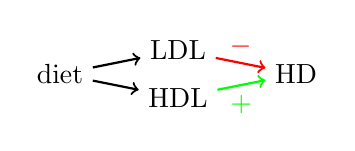
\begin{tikzpicture}
		\node (d1) at(0,0.0) {diet};
		\node (LDL) at(1.5,0.3) {LDL};
		\node (HDL) at(1.5,-0.3) {HDL};
		\node (HD) at(3,0) {HD};
		
		\draw[->,thick] (d1) -- (HDL);
		\draw[->,thick] (d1) -- (LDL);
		\draw[->,red,thick] (LDL) -- node[above,yshift=-1] {$-$} (HD);
		\draw[->,green,thick] (HDL) -- node[below] {$+$} (HD);
		\end{tikzpicture}
		\caption{}\label{fig:cholesterol:a}
	\end{subfigure}
	%
	\hfill
	%
	\begin{subfigure}{.45\linewidth}
		\center\
		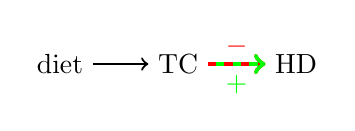
\begin{tikzpicture}
		\node (d1) at(0,0.) {diet};
		\node (LHDL) at(1.5,0) {TC};
		\node (HD) at(3,0) {HD};
		
		\draw[->,thick] (d1) -- (LHDL);
		\draw[->,red,dash pattern= on 3pt off 3pt,ultra thick] (LHDL) -- node[above,yshift=-1] {$-$} (HD);
		\draw[->,green,dash pattern= on 3pt off 3pt,dash phase=3pt,ultra thick] (LHDL) -- node[below] {$+$} (HD);
		\end{tikzpicture}
		\caption{}\label{fig:cholesterol:b}
	\end{subfigure}
	%
	\caption{Effects of cholesterol on risk of heart disease. As illustrated by~(a), the current consensus is that low-density lipoprotein (LDL) has a negative effect on heart disease (HD), while high-density lipoprotein (HDL) has a positive effect on heart disease. Considering total blood cholesterol (TC = LDL + HDL) to be a causal variable as in~(b) leads to problems: two diets promoting raised LDL levels and raised HDL levels respectively have the same effect on TC but opposite effects on heart disease. Hence different studies come to contradictory conclusions about the effect of TC on heart disease.}
	\label{fig:cholesterol}
\end{figure}


%In the following we give an example of the problems that can arise when there exists no consistent correspondence between two causal models, i.\,e.\ neither model can be viewed as an exact transformation of the other. This example falls into category (b) of the differing model levels listed above and was used by~\cite{spirtes2004causal} to illustrate problems in the causal modelling process.


Historically, the level of total blood cholesterol (TC) in a human subject was thought to be an important variable in determining their risk of developing heart disease (HD).
To investigate this, many experiments were carried out in which patients were assigned to different diets in order to raise or lower TC\@.
Conflicting evidence was found by these experiments: some found that higher TC had the effect of lowering HD, while others found the opposite \citep{truswell2010cholesterol,steinberg2011cholesterol}.

The reason for this apparent contradiction is clear with hindsight, but serves to illustrate the care that must be taken when seeking causal relations. 
The current scientific consensus is that there are two types of blood cholesterol, low-density lipoprotein (LDL) and high-density lipoprotein (HDL), which have a negative and positive effect on HD respectively (Figure \ref{fig:cholesterol:a}).
A measurement of TC is in fact a measurement of the sum of LDL and HDL.
Therefore two experiments, one raising LDL levels and the other raising HDL levels, would have the same effect on TC but opposite effects on HD (Figure \ref{fig:cholesterol:b}).

In this example, total blood cholesterol is too `coarse' a variable to have a well-defined causal relation with risk of heart disease. 
However, if it had been possible to affect only one of LDL and HDL through diet, this issue may never have been discovered:
if only HDL could be influenced by diet, the scientific consensus would be that total blood cholesterol is protective against heart disease and no contradictions would have been found.

Similarly, it is conceivable that there are in fact two different types of HDL: a more prevalent form which is protective against heart disease and one present in smaller quantities that has a detrimental impact. 
If the ratio of these two types is constant under any intervention through diet, the negative impact will always be outweighed by the positive impact and so we might never discover the detrimental subtype. 
If this were true, would the statement `increased HDL levels cause reduced risk of heart disease' be rendered false? 
Arguably it would be an oversimplification of the more complicated truth, but it would not be false in that it would correctly predict the outcome of any conceivable diet-based intervention.

This example raises two main points that we will discuss in the rest of this section. The first is that in the real world measurements or observations are always made at some level of detail or coarseness that is somewhat arbitrary. In the next subsection we will outline a variety of ways in which models of different levels of detail naturally arise in a variety of cases and further motivate the study of this fact in a causal setting.
The second is that whether or not a variable is `causally meaningful' is intricately connected to the interventions being considered. If we consider a coarse variable such as TC, we can consistently model causal relations if the interventions considered are sufficiently restricted, but this breaks down if the interventions are too rich. In subsection ?? we will discuss how to modify the framework of SEMs to take this into account.

The remainder of this section sets the stage for section ??, in which we tackle our overarching goal of trying to answer the following questions:
If the true causal mechanisms of the world operate at a very low level of detail (e.g.~atoms), under what conditions can we speak of causal relations at higher levels (e.g.~objects)?
How can we formalise such a notion of consistent modelling in the framework of SEMs?


\subsection{Modelling at different levels of detail}

Physical systems or processes in the real world are complex and can be understood at various levels of detail.
In the previous subsection we discussed the example of cholesterol levels and risk of heart disease.
Although the true mechanisms by which cholesterol affects heart disease are surely very complicated -- for instance, it may be important how cholesterol is distributed throughout the body -- we sought to summarise the micro-level details into a small number of macro-level variables, the total levels of HDL and LDL.

Another example of micro-macro abstraction 
%that is more rigorously understood 
can be found in statistical physics.
A gas in a volume consists of a large number of molecules, but instead of modelling the motions of each particle individually, we may choose to consider macroscopic properties of their motions such as temperature and pressure.
As in the case of cholesterol, our decision to use such macroscopic properties may first necessitated by practical considerations.
Indeed, for all but extremely simple cases, making a measurement of all the individual molecules is practically impossible and our resources insufficient for modelling the ${\sim}10^{22}$ particles present per litre of ideal gas.
Furthermore, the decision for a macroscopic description level is also a pragmatic one: if we only wish to reason about temperature and pressure, a model of $10^{22}$ particles is ill-suited.

Statistical physics explains how higher-level concepts such as temperature and pressure arise as statistical properties of a system of a large number of particles, justifying the use of a macro-level model as a useful transformation of the micro-level model~\citep{Balian}.
However, in many cases aggregate or indirect measurements of a complex system form the basis of a macroscopic description of the system, with little theory to explain whether this is justified or how the micro- and macro-descriptions stand in relation to each other.

Due to deliberate modelling choice or the limited ability to observe a system, differing levels of model descriptions are ubiquitous and occur, amongst possibly others, in the following three settings:

\begin{itemize}[noitemsep]
	\item[(a)] Models with large numbers of variables versus models in which the `irrelevant' or unobservable variables have been marginalised out \citep{bongers2016structural}; e.\,g.\ modelling blood cholesterol levels and risk of heart disease while ignoring other blood chemicals or external factors such as stress.
	
	\item[(b)] Micro-level models versus macro-level models in which the macro-variables are aggregate features of the micro-variables \citep{simon1961aggregation,iwasaki1994causality,hoel2013quantifying,chalupka2015visual,chalupka2016multi}; e.\,g.\ instead of modelling the brain as consisting of $100$ billion neurons it can be modelled as averaged neuronal activity in distinct functional brain regions.
	
	\item[(c)] Dynamical time series models versus models of their stationary behaviour \citep{fisher1970correspondence,iwasaki1994causality,dash2001caveats,lacerda2012discovering,mooij2013ode,mooij2013cyclic}; e.\,g.\ modelling only the final ratios of reactants and products of a time evolving chemical reaction.
\end{itemize}

In the context of causal modelling, such differing model levels should be consistent with one another in the sense that they agree in their predictions of the effects of interventions. 
In section ??, the notion of an exact transformation between two SEMs is introduced, providing a general framework to evaluate when two models can be thought of as causal descriptions of the same system.
On a high level, if an SEM can be viewed as an exact transformation of another SEM, there is an explicit correspondence between the two models in such a way that causal reasoning on both levels is consistent.


%The particular causal models we focus on in this paper are Structural Equation Models (SEMs, Section~\ref{sec:SEMs}, Section~\ref{sec:sem-for-causal-modelling}) \citep{spirtes2000causation,pearl2009causality}.
%
%In Section~\ref{sec:sem-transformation}, we introduce the notion of an exact transformation between two SEMs, providing us with a general framework to evaluate when two models can be thought of as causal descriptions of the same system.
%An important novel idea of this paper is to explicitly make use of a natural ordering on the set of interventions.
%On a high level, if an SEM can be viewed as an exact transformation of another SEM, we are provided with an explicit correspondence between the two models in such a way that causal reasoning on both levels is consistent.
%We discuss this notion of consistency in detail in Sections~\ref{subsec:causal-interpretation-transformation} and~\ref{sec:wrong}.
%
%In Section~\ref{sec:example-transformations} we apply this mathematical framework and prove the exactness of transformations belonging to each of the three categories listed above, with practical implications for the following questions in causal modelling:
%When can we model only a subsystem of a more complex system?
%When does a micro-level system admit a causal description in terms of macro-level features?
%How do cyclic SEMs arise?
%The fact that these distinct problems can all be considered using the language of transformations between SEMs demonstrates the generality of our approach.
%We close in Section~\ref{sec:questions} with a discussion.


%It is therefore not possible to transform the model in Figure~\ref{fig:cholesterol:b} into the model in Figure~\ref{fig:cholesterol:a} without leading to conflict:
%in order to reason about the causes of HD we need to consider the variables LDL and HDL separately.

\subsection{Natural partial orderings on interventions}

We next introduce an important novel idea that must be discussed before exact transformations can be formally defined.
This is to extend the definition of SEMs to explicitly include restricted sets of interventions and to introduce a natural ordering that exists on such sets of interventions.






\section{Transformations between Structural Equation Models}
\section{Examples of transformations}
\section{Discussion and work building on this}











































%
%!TEX root = ../thesis.tex
%*******************************************************************************
%****************************** Third Chapter **********************************
%*******************************************************************************
\chapter{Conclusion}\label{chapter:conclusion}

% **************************** Define Graphics Path **************************
\ifpdf
    \graphicspath{{Chapter7/Figs/Raster/}{Chapter7/Figs/PDF/}{Chapter7/Figs/}}
\else
    \graphicspath{{Chapter7/Figs/Vector/}{Chapter7/Figs/}}
\fi

This thesis presented theoretical advances in three niches of the machine learning literature related to the modelling of structured data.
This chapter summarises the main contributions and discusses future directions of research.

\section{Summary of Contributions}

Chapter \ref{chapter:latent-space-learning-theory} presented an estimator for $f$-divergences between pairs of distributions satisfying certain structural assumptions that are naturally satisfied in the setting of autoencoders. 
These assumptions enabled the derivation of fast rates for the decay of the bias and concentration of this estimator without additional strong assumptions on the distributions.
This is in contrast to much of the existing $f$-divergence estimation literature, where fast rates are only attainable with strong assumptions that would be difficult to verify in practice.

%These assumptions that hold in this setting make it possible to estimate the divergences with fast rates.
%In contrast, in much of the existing $f$-divergence estimation literature fast rates are only attainable with strong assumptions that would be hard to verify in practice.

Chapter \ref{chapter:ica} presented identifiability results for a novel multi-view nonlinear ICA setting, extending the few identifiability results known for nonlinear ICA.
These results required at least one of the views to exhibit source-side noise, termed corruptions.
In particular, if one noiseless view of the sources is supplemented by a second view that is appropriately corrupted by source-level noise, it was proved that the sources can be fully reconstructed from the observations up to tolerable ambiguities.
%The settings considered were: one in which two views are available, one of which is noiseless, in which case full reconstruction of the sources is possible; one in which two noisy views are available, in which reconstruction of the sources up to the corruptions is possible; one in which a large number of noisy views are available, in which case preliminary results suggest
This setting has application to practical scenarios in which multiple distinct data modalities are available, such as in neuroimaging. % where fMRI and EEG data of a subject may be measured.


Chapter \ref{chapter:causality} introduced the notion of \emph{exact transformations} between Structural Equations Models (SEMs), providing a framework to understand when two SEMs can be viewed as consistent causal models of the same system at different levels of detail. 
This provides a way to formally understand when higher-level variables can be considered to be causal variables, and encompasses a wide range of settings in which such higher-level models arise.
Practically all measurements are made at a level of detail different to that at which `true' causal structure exists, yet causal discovery algorithms typically seek causal relations at the level of measurements.
Thus, this work has broad implications to the causality community in general and in particular to the problem of causal variable definition.
It furthermore brings to attention the importance of the specification of interventions of interest as a part of the causal modelling process.


\section{Future directions}

Chapter \ref{chapter:latent-space-learning-theory} was fundamentally a learning theoretic study of $f$-divergence estimation under particular structural assumptions. 
One direction for future enquiry would be the use of the proposed RAM-MC estimator for optimisation, instead of pure estimation. 
A clear application of this would be to the training of Wasserstein Autoencoders, the regularisation term of which is any divergence between the prior and aggregate posterior, and naturally satisfies the structural assumptions considered in this chapter.

This work has broader implications as it demonstrates that there is interesting work to be done at the intersection of deep learning and learning theory. 
While the learning theory literature has tended to focus on settings in which as few assumptions are made as possible, this work shows that in some cases strong assumptions that naturally apply to modern deep learning settings can yield superior results.
To give one specific example, it is known that in the general case, estimation of mutual information is a hard problem \citep{mcallester2018formal}.
Yet in many practical cases where mutual information is used, such as in representation learning \citep{hjelm2018learning, oord2018representation, tschannen2020onmutual}, stronger assumptions may hold than in the general case.
One such setting was encountered in Chapter \ref{chapter:latent-space-learning-theory}, though others may exist.

The identifiability results presented in Chapter \ref{chapter:ica} show that ICA in the multi-view setting is in principle possible, and natural next steps would be the development of practical algorithms that actually work in application.
%Tbut it remains to be seen whether the proposal works in practice.
%If not, other approaches can be considered; identifiability results have been proven and so t

An emerging area within deep learning is \emph{disentangled representation learning}. 
This empirically driven community shares similar goals to the ICA community but with a strong emphasis on image datasets.
Despite this, few bridges have been built between the two communities, though recent work in  disentanglement has begun to consider multi-view settings similar to that considered here \citep{shu2019weakly}.

One barrier to connecting the ICA and disentanglement communities is the pervasive assumption in ICA that the source and observation dimensions be the same.
In high dimensional data such as images, this is clearly unrealistic as usually dozens of latent dimensions are sufficient to explain the majority of variation in images with hundreds or thousands of pixels. 
Thus, attempting to relax this assumption would seem to be a possible way to give ICA wider applicability across the modern machine learning community.


Similarly, gaps exist between the causality literature and modern advances in deep learning.
The fundamental assumption to almost all causal learning algorithms is that the individual components of the data are meaningful entities. 
In contrast, deep learning algorithms can be applied to data such as images and audio for which the components of raw data, i.e. individual pixels or amplitudes at a particular point in time, are themselves not meaningful, but where higher-level features such as objects, textures or syllables are.
Causality is nonetheless gaining increasing attention outside of the traditional community, with authors such as \cite{bengio2019meta} attempting to blend ideas from causality with deep learning.

The framework introduced in Chapter \ref{chapter:causality} allows one to reason about whether higher-level causal variables are consistent with the `raw' variables from which they are derived, but it is not clear how such coarsenings can be learned automatically from data.
My hope is that others may build on this work, leading to `causal' feature learning.
However, given the central importance of interventions in the causal setting, I have reservations about whether this is possible given the current paradigm of \iid~machine learning with large datasets.
Reinforcement learning, however, could be a fruitful area in which to apply ideas from causality, given the centrality of action there.




%\begin{itemize}
%	\item What was presented in this thesis?
%	\item How are the contributions in this thesis connected to current areas of advancement?
%\end{itemize}



% ********************************** Back Matter *******************************
% Backmatter should be commented out, if you are using appendices after References
%\backmatter

% ********************************** Bibliography ******************************
\begin{spacing}{0.9}

% To use the conventional natbib style referencing
% Bibliography style previews: http://nodonn.tipido.net/bibstyle.php
% Reference styles: http://sites.stat.psu.edu/~surajit/present/bib.htm

%\bibliographystyle{apalike}
%\bibliographystyle{unsrt} % Use for unsorted references  
%\bibliographystyle{plainnat} % use this to have URLs listed in References
\cleardoublepage
%\bibliography{References/references} % Path to your References.bib file


% If you would like to use BibLaTeX for your references, pass `custombib' as
% an option in the document class. The location of 'reference.bib' should be
% specified in the preamble.tex file in the custombib section.
% Comment out the lines related to natbib above and uncomment the following line.

\printbibliography[heading=bibintoc, title={References}, notcategory=ignore]


\end{spacing}

% ********************************** Appendices ********************************

\begin{appendices} % Using appendices environment for more functunality

%!TEX root = ../thesis.tex
% ******************************* Thesis Appendix B ********************************

\ifpdf
    \graphicspath{{Appendix3/Figs/Raster/}{Appendix3/Figs/PDF/}{Appendix3/Figs/}}
\else
    \graphicspath{{Appendix3/Figs/Vector/}{Appendix3/Figs/}}
\fi


\chapter{Additional Materials for Chapter \ref{chapter:latent-space-learning-theory}}\label{chapter:appendix-latex-space-learning-theory}

\section{Proof of Proposition \ref{prop:upper-bound}}\label{proof:prop1}

\begin{repproposition}{prop:upper-bound}
Let $M \leq N$ be integers. Then
\begin{align*}
    D_f(Q_Z , P_Z) \ \leq 
    \mathbb{E}_{\mathbf{X}^N \sim Q_{X}^N} D_f( \hat{Q}_Z^N , P_Z) \  \leq \ \mathbb{E}_{\mathbf{X}^M \sim Q_{X}^M} D_f( \hat{Q}_Z^M , P_Z).
\end{align*}
\end{repproposition}
\begin{proof}
Observe that $\mathbb{E}_{\mathbf{X}^N} \hat{Q}_Z^N = Q_Z$. Thus,
\begin{align*}
    D_f(Q_Z , P_Z) &= \int f\left(\frac{\E_{\XN}\hat{q}_N(z)}{p(z)}\right) dP_Z(z) \\
    &\leq \E_{\XN} \int f\left(\frac{\hat{q}_N(z)}{p(z)}\right) dP_Z(z)\\
    &=\mathbb{E}_{\mathbf{X}^N \sim Q_{X}^N} D_f( \hat{Q}_Z^N , P_Z),
\end{align*}
where the inequality follows from convexity of $f$.

To see that $\mathbb{E}_{\mathbf{X}^N \sim Q_{X}^N} D_f( \hat{Q}_Z^N , P_Z) \leq \mathbb{E}_{\mathbf{X}^M \sim Q_{X}^N} D_f( \hat{Q}_Z^M , P_Z)$ for $N \geq M$,
let $I \subseteq \{1, \ldots, N\}$, $|I| = M$ and write
\begin{align*}
    \hat{Q}_Z^I = \frac{1}{M} \sum_{i \in I} Q_{Z | X_i}.
\end{align*}
%
Letting $I$ be a random subset chosen uniformly \emph{without replacement},
observe that for any fixed $I$, $\mathbf{X}^I \sim Q_X^M$ (with the randomness coming from $\mathbf{X}^N \sim Q_X^N$). Thus
%
\begin{align*}
    \hat{Q}_Z^N &= \frac{1}{N} \sum_{i=1}^N Q_{Z|X_i} \\
    &= \mathbb{E}_I \frac{1}{M} \sum_{i \in I} Q_{Z|X_i} \\
    &= \mathbb{E}_I \hat{Q}_Z^I
\end{align*}
%
and so again by convexity of $f$ we have that
%
\begin{align*}
    \mathbb{E}_{\mathbf{X}^N \sim Q_{X}^N} D_f( \hat{Q}_Z^N , P_Z) &\leq  \mathbb{E}_{\mathbf{X}^N} \mathbb{E}_I D_f( \hat{Q}_Z^I , P_Z) \\
    &= \mathbb{E}_{\mathbf{X}^M} D_f(\hat{Q}_Z^M , P_Z)
\end{align*}
with the last line following from the observation that $\mathbf{X}^I \sim Q_X^M$.
\end{proof}



\section{Proof of Theorem \ref{thm:fast-KL-rate}}\label{appendix:subsec:thm1}




\begin{reptheorem}{thm:fast-KL-rate}[Rates of the bias]
If
$\E_{X\sim Q_X}\bigl[\chi^2\bigl(Q_{Z|X}, Q_Z\bigr)\bigr]$ and
$\KL\left( Q_{Z} , P_Z\right)$ are finite then the bias ${\E_{\XN}\bigl[D_f( \hat{Q}_Z^N , P_Z)\bigr] - D_f\left( Q_{Z} , P_Z\right)}$ decays with rate as given in the first row of Table~\ref{table:convergence} (see Page \pageref{table:convergence}).
\end{reptheorem}

\begin{proof}
To begin, observe that 
\begin{align*}
    \E_{\XN}\left[\chi^2\bigl(\hat{Q}^N_Z, Q_Z\bigr)\right]
    &= \E_{\XN}\E_{Q_Z}\left[\left(\frac{\hat{q}_N(z)}{q(z)} - 1\right)^2 \right]\\
    &=\E_{Q_Z} \V_{\XN} \left[ \frac{1}{N} \sum_{n=1}^N\frac{q(z|X_n)}{q(z)}\right] \\
    &= \frac{1}{N} \E_{Q_Z}\V_X \left[ \frac{q(z|X)}{q(z)} \right]\\
    &= \frac{1}{N}\E_{X}\left[\chi^2\bigl(Q_{Z|X}, Q_Z\bigr) \right]
\end{align*}

where the introduction of the variance operator follows from the fact that $\E_{X_N}\left[ \frac{\hat{q}_N(z)}{q(z)} \right] = 1$.

For the $\KL$-divergence, using the fact that $\KL \leq \chi^2$ (Lemma \ref{lemma:f-div-klleqchi}) yields
\begin{align*}
    \E_{\XN}\left[\KL\left( \hat{Q}^N_Z , P_Z\right)\right] - \KL\left( Q_{Z} , P_Z\right) &=\E_{\XN}\left[\KL\left( \hat{Q}^N_Z , Q_Z\right)\right]\\
    &\leq \E_{\XN}\left[\chi^2\bigl(\hat{Q}^N_Z, Q_Z\bigr) \right]\\
    &= \frac{1}{N}\E_{X}\left[\chi^2\bigl(Q_{Z|X}, Q_Z\bigr)\right]\\
    &=O\left(\frac{1}{N}\right),
\end{align*}
where the first equality can be verified by using the definition of $\KL$ and the fact that $Q_Z = \E_{\XN}\hat{Q}^N_Z$.

For Total Variation, we have
\begin{align*}
    \E_{\XN}\left[\TV\left( \hat{Q}^N_Z , P_Z\right)\right] - \TV\left( Q_{Z} , P_Z\right) &\leq\E_{\XN}\left[\TV\left( \hat{Q}^N_Z , Q_Z\right)\right]\\
    &\leq \frac{1}{\sqrt{2}} \sqrt{\E_{\XN}\left[\KL\left( \hat{Q}^N_Z , Q_Z\right) \right]}\\
    &=O\left(\frac{1}{\sqrt{N}}\right),
\end{align*}
where the first inequality holds since $\TV$ is a metric and thus obeys the triangle inequality, and the second inequality follows by Pinsker's inequality combined with concavity of $\sqrt{x}$ (Lemma \ref{lemma:f-div-pinsker}).

For $D_{f_\beta}$ (including Jenson-Shannon) using the fact that $D_{f_\beta}^{1/2}$ satisfies the triangular inequality, we apply the second part of Lemma~\ref{lemma:hilbertian-triangle}
in combination with the fact that
$D_{f_\beta}\left(\hat{Q}^N_Z , Q_Z\right) \leq \psi(\beta) \ \TV\left( \hat{Q}^N_Z , Q_Z \right)$ for some scalar $\psi(\beta)$ (Lemma \ref{lemma:f-div-betaleqtv}) to obtain
%
\begin{align*}
    \E_{\XN}\left[D_{f_\beta}\left( \hat{Q}^N_Z , P_Z\right)\right] - D_{f_\beta}\left( Q_{Z} , P_Z\right) \leq O\left(\frac{1}{N^{1/4}}\right).
\end{align*}
%
Although the squared Hellinger divergence is a member of the $f_\beta$-divergence family, we can use the tighter bound $\Hsq\left( \hat{Q}^N_Z , Q_Z\right) \leq KL\left( \hat{Q}^N_Z , Q_Z\right)$ (Lemma \ref{lemma:f-div-hleqkl}) in combination with Lemma~\ref{lemma:hilbertian-triangle} to obtain
\begin{align*}
    \E_{\XN}\left[\Hsq\left( \hat{Q}^N_Z , P_Z\right)\right] - \Hsq\left( Q_{Z} , P_Z\right) \leq O\left(\frac{1}{\sqrt{N}}\right).
\end{align*}
\end{proof}





\section{Upper bounds of f}\label{appendix:subsubsec:f-upper-bounds}

We will make use of the following lemmas in the proofs of Theorem \ref{thm:convergence-rate-general} and \ref{thm:concentration}.

\medskip

\begin{lemma}\label{lemma:concave-upper-bound-kl} 
Let $f_0(x)=x\log x - x +1$, corresponding to $D_{f_0} = \KL$.
Write $g(x) = f_0'^2(x) = \log^2(x)$.
For any $0< \delta < 1$, the function
\begin{align*}
    h_{\delta}(x) := \begin{cases} 
    g(\delta) + x g'(e) & \: x \in [0, e]\\
    g(\delta) + e g'(e) + g(x) - g(e) & \: x \in [e, \infty)
    \end{cases}
\end{align*}
is an upper bound of $g(x)$ on $[\delta, \infty)$, and is concave and non-negative on $[0, \infty)$.
\end{lemma}

\begin{proof}
First observe that $h_{\delta}$ is concave.
It has continuous first and second derivatives:
\begin{align*}
    h_{\delta}'(x) = \begin{cases} 
    g'(e) & \: x \in [0, e]\\
    g'(x) & \: x \in [e, \infty)
    \end{cases}
    &&
    h_{\delta}''(x) = \begin{cases} 
    0 & \: x \in [0, e]\\
    g''(x) & \: x \in [e, \infty)
    \end{cases}
\end{align*}
Note that $g''(x) = \frac{2}{x^2} - \frac{2 \log(x)}{x^2} \leq 0$ for $x \geq e$ and $g''(e) = 0$.
Therefore $h''_{\delta}(x)$ has non-positive second derivative on $[0, \infty)$ and is thus concave on this set.

To see that $h_{\delta}(x)$ is an upper bound of $g(x)$ for $x \in [\delta, \infty)$, use the fact that $g'(x) = \frac{2\log(x)}{x}$ and observe that
\begin{align*}
    h_{\delta}(x) - g(x)
    &= \begin{cases} 
    \log^2(\delta) + \frac{2x}{e} - \log^2(x)& \: x \in [\delta, e]\\
    \log^2(\delta) + 1& \: x \in [e, \infty)
    \end{cases}
    \ > 0.
\end{align*}
%
To see that $h_{\delta}(x)$ is non-negative on $[0, \infty)$, note that $h_{\delta}(x) > g(x) \geq 0$ on $[\delta, \infty)$. 
Moreover, $g'(e) = 2/e > 0$, and so for $x \in [0, \delta]$ we have that $h_{\delta}(x) = g(\delta) + 2x/e \geq g(\delta) \geq 0$.
\end{proof}

\medskip

\begin{lemma}\label{lemma:upper-bound-hellinger}
Let $f_0(x) = 2(1 -\sqrt{x})$ corresponding to the squared-Hellinger divergence. 
Write $g(x) = f'^2_0(x) = (1-\frac{1}{\sqrt{x}})^2$.
For any $0<\delta<1$, the function
\begin{align*}
    h_\delta(x) = \frac{1}{\delta}(x-1)^2 
\end{align*}
is an upper bound of $g(x)$ on $[\delta, \infty)$.
\end{lemma}
\begin{proof}
For $x=1$, we have $g(1)=h_\delta(1)$. 
For $x\not=1$,
\begin{align*}
    0 &\leq \frac{1}{\delta}(x-1)^2 - (1-\frac{1}{\sqrt{x}})^2 \\
    \iff \sqrt{\delta} &\leq \frac{x-1}{1-\frac{1}{\sqrt{x}}}
\end{align*}
If $x \in [\delta, 1)$ then
\begin{align*}
    \frac{x-1}{1-\frac{1}{\sqrt{x}}} &= \sqrt{x} \cdot \frac{\frac{1}{\sqrt{x}} - \sqrt{x}}{\frac{1}{\sqrt{x}}-1} \geq \sqrt{x} \geq \sqrt{\delta}.
\end{align*}
If $x \in (1, \infty)$ then
\begin{align*}
    \frac{x-1}{1-\frac{1}{\sqrt{x}}} &= \sqrt{x} \cdot \frac{\sqrt{x} - \frac{1}{\sqrt{x}}}{1-\frac{1}{\sqrt{x}}} \geq \sqrt{x} \geq \sqrt{\delta}.
\end{align*}
Thus $g(x) \leq h_\delta(x)$ for $x\in[\delta, \infty)$.
\end{proof}

\medskip

\begin{lemma}\label{lemma:upper-bound-alpha}
Let $f_0(x) = \frac{4}{1-\alpha^2}\left(1 -x^{\frac{1+\alpha}{2}}\right) - \frac{2(x-1)}{\alpha-1}$ corresponding to the $\alpha$-divergence with $\alpha \in (-1,1)$. 
Write $g(x) = f'^2_0(x) = \frac{4}{(\alpha -1)^2} \left(x^\frac{\alpha-1}{2} - 1\right)^2$.
For any $0<\delta<1$, the function
\begin{align*}
    h_\delta(x) = \frac{4\left(\delta^\frac{\alpha-1}{2} - 1\right)^2}{(\alpha - 1)^2 (\delta- 1)^2}\cdot (x-1)^2
\end{align*}
is an upper bound of $g(x)$ on $[\delta, \infty)$.
\end{lemma}
\begin{proof}
For $x=1$, we have $g(1)=h_\delta(1)$. 
Consider now the case that $x\geq\delta$ and $x\not=1$. 
Since $0<\delta <1$, we have that $1-\delta > 0$.
And because $(\alpha-1)/2 \in (-1,0)$, we have that $\delta^{\frac{\alpha - 1}{2}} - 1 > 0$.
It follows by taking square roots that
\begin{align*}
    &g(x) \leq h_\delta(x) \\
    \iff& d(x) := \frac{x^{\frac{\alpha -1}{2}} -1}{1-x} \leq \frac{\delta^{\frac{\alpha -1}{2}} -1}{1-\delta} 
\end{align*}
Now, $d(x)$ is non-increasing for $x>0$. Indeed,
\begin{align*}
    d'(x) = \frac{-1}{(1-x)^2} \left[ 1 - \frac{3 - \alpha}{2}x^{\frac{\alpha -1}{2}} + \frac{1-\alpha}{2} x^{\frac{\alpha-3}{2}} \right]
\end{align*}
and it can be shown by differentiating that the term inside the square brackets attains its minimum at $x=1$ and is therefore non-negative. Since $(1-x)^2 \geq 0$ it follows that $d'(x) \leq 0$ and so $d(x)$ is non-increasing.
From this fact it follows that $d(x)$ attains its maximum on $x \in [\delta, \infty)$ at $x=\delta$, and thus the desired inequality holds. 
\end{proof}

\medskip

\begin{lemma}\label{lemma:upper-bound-JS}
Let $f_0(x) = \left(1+x\right) \log 2 + x\log x - \left( 1 + x\right) \log \left(1+x\right)$ corresponding to the Jensen-Shannon divergence.
Write $g(x) = f'^2_0(x) = \log^2 2 + \log^2\left( \frac{x}{1+x} \right) + 2\log 2 \log\left( \frac{x}{1+x} \right)$.
For $0< \delta < 1$, the function
\begin{align*}
    h_\delta(x) = g(\delta) + 4\log^2 2
\end{align*}
is an upper bound of $g(x)$ on $[\delta, \infty)$.
\end{lemma}
\begin{proof}
For $x\geq1$,  $\frac{x}{x+1} \in [0.5, 1)$ and so $\log\left( \frac{x}{1+x} \right) \in \left[-\log2, 0\right)$.
Therefore $g(x) \in \left(0, 4\log^2 2\right]$ for $x>1$.
It follows that for any value of $\delta$, $h_\delta(x) \geq g(x)$ for $x\geq1$.
$f'_0(1)=0$ and by differentiating again it can be shown that $f''_0(x) > 0$ for $x\in(0,1)$.
Thus $f'_0(x)<0$ and is increasing on $(0,1)$ and so $g(x) > 0$ and is decreasing on $(0,1)$.
Thus $h_\delta(x) > g(\delta) \geq g(x)$ for $x \in [\delta, 1)$.
\end{proof}

\medskip

\begin{lemma}\label{lemma:upper-bound-f-beta}
Let $f_0(x) = \frac{1}{1-\frac{1}{\beta}}\left[ \left(1+x^\beta\right)^\frac{1}{\beta}  - 2^{\frac{1}{\beta} - 1}(1+x)\right]$
corresponding to the ${f_\beta}$-divergence introduced in \cite{osterreicher2003new}.
We assume $\beta \in \left( \frac{1}{2}, \infty\right) \setminus \{1\}$.
Write $g(x) = f'^2_0(x) = \left(\frac{\beta}{1-\beta}\right)^2\left[ \left(1+x^{-\beta}\right)^\frac{1-\beta}{\beta}  - 2^{\frac{1}{\beta} - 1}\right]^2$.

If $\beta \in \left(\frac{1}{2}, 1\right)$, then $\lim_{x\to \infty}g(x)$ exists and is finite and for any $0<\delta<1$, we have that $h_\delta(x) := g(\delta) + \lim_{x\to \infty}g(x) \geq g(x)$ for all $x\in[\delta, \infty)$.

If $\beta \in \left(1, \infty \right)$, then $\lim_{x\to0}g(x)$ and $\lim_{x\to \infty}g(x)$ both exist and are finite, and $g(x) \leq \max\{\lim_{x\to0}g(x), \lim_{x\to \infty}g(x)\}$ for all $x\in[0, \infty)$.
\end{lemma}
\begin{proof}
For any $\beta \in \left( \frac{1}{2}, \infty\right) \setminus \{1\}$, we have that $f''_0(x) = \frac{\beta}{(1-\beta)^2} \left[ 
\frac{1}{x^{\beta+1}} \left( 1 + x^{-\beta}\right)^{\frac{1-2\beta}{\beta}}\right] > 0$ for $x>0$.
Since $f'_0(1)=0$, it follows that $f'_0(x)$ is increasing everywhere, negative on $(0,1)$ and positive on $(1,\infty)$.
It follows that $g(x)$ is decreasing on $(0,1)$ and increasing on $(1,\infty)$.
$\beta > 0$ means that $1+x^{-\beta} \to 1$ as $x\to \infty$. Hence $g(x)$ is bounded above and increasing in $x$, thus $\lim_{x\to\infty} g(x)$ exists and is finite.

For $\beta \in (\frac{1}{2}, 1)$, $\frac{1-\beta}{\beta} > 0$. 
It follows that $\left(1+x^{-\beta}\right)^\frac{1-\beta}{\beta}$ grows unboundedly as $x \to 0$, and hence so does $g(x)$.
Since $g(x)$ is decreasing on $(0,1)$, for any $0<\delta<1$ we have that $h_\delta(x)\geq g(x)$ on $(0,1)$.
Since $g(x)$ is increasing on $(1, \infty)$ we have that $h_\delta(x) \geq \lim_{x\to\infty} g(x) \geq g(x)$ on $(1,\infty)$.

For $\beta \in (1, \infty)$, $\frac{1-\beta}{\beta} < 0$. 
It follows that $\left(1+x^{-\beta}\right)^\frac{1-\beta}{\beta} \to 0$ as $x \to 0$, and hence $\lim_{x\to 0}g(x)$ exists and is finite.
Since $g(x)$ is decreasing on $(0,1)$ and increasing on $(1,\infty)$, it follows that 
$g(x) \leq \max\{\lim_{x\to 0}g(x), \lim_{x\to \infty}g(x)\}$ for all $x\in [0, \infty)$
\end{proof}


\section{Proof of Theorem \ref{thm:convergence-rate-general}}\label{proof:thm2}

\begin{reptheorem}{thm:convergence-rate-general}[Rates of the bias]
If $\E_{X\sim Q_X, Z\sim P_Z}\bigl[ q^4(Z|X) / p^4(Z) \bigr]$ is finite then
the bias $\E_{\XN}\bigl[D_f( \hat{Q}_Z^N , P_Z)\bigr] - D_f\left( Q_{Z} , P_Z\right)$ decays with rate as given in the second row of Table \ref{table:convergence} (see Page \pageref{table:convergence}).
\end{reptheorem}

\begin{proof}
For each $f$-divergence we will work with the function $f_0$ which is decreasing on $(0,1)$ and increasing on $(1, \infty)$ with $D_f = D_{f_0}$ (see Section \ref{subsec:f-divergences-intro}).

For shorthand we will sometimes use the notation $\| q(z|X)/p(z)\|^2_{L_2(P_Z)} = \int \frac{q(z|X)^2}{p(z)^2} p(z) dz$ and $\| q^2(z|X)/p^2(z)\|^2_{L_2(P_Z)} = \int \frac{q(z|X)^4}{p(z)^4} p(z) dz$.

We will denote $C:= \E_{X\sim Q_X, Z\sim P_Z}\bigl[ q^4(Z|X) / p^4(Z) \bigr]$ which is finite by assumption. 
This implies that the second moment $B:= \E_{X\sim Q_X, Z\sim P_Z}\bigl[ q^2(Z|X) / p^2(Z) \bigr]$ is also finite due to Jensen's inequality: 
\[
\E[Y^2] = \E[\sqrt{Y^4}]\leq \sqrt{\E[Y^4]}.
\]

% New proof for chi^2
\paragraph{The case that $D_f$ is the $\chi^2$-divergence:}
% 
In this case, using $f(x) = x^2-1$, it can be seen that the bias is equal to
\begin{align}\label{eqn:chi2-bias}
    \E_{\XN} \left[ D_{f}\left( \hat{Q}_Z^N , P_Z\right)\right] - D_{f}\left( Q_{Z} , P_Z\right) = \E_{\XN}\left[ \int_Z  \left(\frac{\hat{q}_N(z) - q(z)}{p(z)}\right)^2 dP(z) \right].
\end{align}
Indeed, expanding the right hand side and using the fact that $\E_{\XN}\hat{q}_N(z) = q(z)$ yields
\begin{align*}
    &\E_{\XN}\left[ \int_Z  \frac{\hat{q}^2_N(z) - 2\hat{q}_N(z)q(z) + q^2(z)}{p^2(z)} dP(z) \right]\\
    &=\E_{\XN}\left[ \int_Z  \frac{\hat{q}^2_N(z) - q^2(z)}{p^2(z)} dP(z) \right]\\
    &=\E_{\XN}\left[ \int_Z  \left(\frac{\hat{q}^2_N(z)}{p^2(z)} - 1 \right)dP(z) \right] - \int_Z  \left(\frac{q^2(z)}{p^2(z)} - 1\right) dP(z)\\
    &= \E_{\XN} \left[ D_{f}\left( \hat{Q}_Z^N , P_Z\right)\right] - D_{f}\left( Q_{Z} , P_Z\right).
\end{align*}
Again using the fact that $\E_{\XN}\hat{q}_N(z) = q(z)$, observe that taking expectations over $\XN$ in the right hand size of Equation \ref{eqn:chi2-bias} above (after changing the order of integration) can be viewed as taking the variance of $\hat{q}_N(z)/p(z)$, the average of $N$ i.i.d. random variables, and so

\begin{align*}
 \E_{\XN}\left[ \int_Z  \left(\frac{\hat{q}_N(z) - q(z)}{p(z)}\right)^2 dP(z) \right] &= \int_Z \E_{\XN}\left[  \left(\frac{\hat{q}_N(z) - q(z)}{p(z)}\right)^2 \right] dP(z) \\
 &=\frac{1}{N} \int_Z \E_{X}\left[  \left(\frac{q(z|X) - q(z)}{p(z)}\right)^2 \right] dP(z) \\
 &= \frac{1}{N} \E_{X} \chi^2\left( Q_{Z|X} , P_Z \right) - \frac{1}{N} \chi^2\left( Q_{Z} , P_Z \right)\\
 &\leq \frac{B-1}{N}.
\end{align*}

\paragraph{The case that $D_f$ is the Total Variation distance or $D_{f_\beta}$ with $\beta>1$:}

For these divergences, we only need the condition that the second moment $\E_X \| q(z|X)/p(z)\|^2_{L_2(P_Z)} < \infty$ is bounded.

\begin{align*}
    & \E_{\XN} \left[ D_{f_0}\left( \hat{Q}_Z^N , P_Z\right)\right] - D_{f_0}\left( Q_{Z} , P_Z\right)  \\
    &= \E_{\XN}\E_{P_Z} \left[ f_0\left( \frac{\hat{q}_N(z)}{p(z)} \right) - f_0\left( \frac{q(z)}{p(z)} \right) \right] \\
    &\leq \E_{\XN}\E_{P_Z} \left[ \left( \frac{\hat{q}_N(z) - q(z)}{p(z)} \right)     f_0'\left(\frac{\hat{q}_N(z)}{p(z)} \right) \right]  \\
    &\leq \underbrace{ \sqrt{ \E_{\XN}\E_{P_Z} \left[\left( \frac{\hat{q}_N(z) - q(z)}{p(z)} \right)^2\right] }}_{(i)} 
    \times 
    \underbrace{\sqrt{\E_{\XN}\E_{P_Z} \left[ f_0'^2\left(\frac{\hat{q}_N(z)}{p(z)}\right] \right) }}_{(ii)}
\end{align*}
where the first inequality holds due to convexity of $f_0$ and the second inequality follows by Cauchy-Schwartz.
Then,
\begin{align*}
    (i)^2 
    &= \E_{P_Z} \text{Var}_{\XN}\left[\frac{\hat{q}_N(z)}{p(z)} \right]\\
    &= \frac{1}{N}\E_{P_Z} \text{Var}_{X}\left[\frac{q(z|X)}{p(z)} \right]\\
    &\leq \frac{1}{N}\E_{X} \E_{P_Z} \left[ \frac{q^2(z|X)}{p^2(z)} \right] = \frac{1}{N} \E_X \left\| \frac{q(z|X)}{p(z)} \right\|^2_{L_2(P_Z)}\\
    \implies & (i) = O\left(\frac{1}{\sqrt{N}}\right).
\end{align*}

For Total Variation, ${f'_0}^2(x) \leq 1$, so
\begin{align*}
    (ii)^2 \leq 1.
\end{align*}

For $D_{f_\beta}$ with $\beta>1$, Lemma~\ref{lemma:upper-bound-f-beta} shows that $f'^2_0(x) \leq \max\{\lim_{x\to 0}f'^2_0(x), \lim_{x\to \infty}f'^2_0(x)\} < \infty$ and so 
\begin{align*}
    (ii)^2 = O(1).
\end{align*}

Thus, for both cases considered,
\begin{align*}
    \E_{\XN} \left[ D_f\left( \hat{Q}_Z^N , P_Z\right)\right] - D_f\left( Q_{Z} , P_Z\right) \leq O\left( \frac{1}{\sqrt{N}} \right).
\end{align*}

\paragraph{All other divergences.}

We start by writing the difference as the sum of integrals over mutually exclusive events that partition $\mathcal{Z}$.
Denoting by $\gamma_N$ and $\delta_N$ scalars depending on $N$, write

\begin{align*}
    & \E_{\XN} \left[ D_f\left( \hat{Q}_Z^N , P_Z\right)\right] - D_f\left( Q_{Z} , P_Z\right)  \\
    &= \E_{\XN} \left[\int f_0\left( \frac{\hat{q}_N(z)}{p(z)} \right) - f_0\left( \frac{q(z)}{p(z)} \right) dP_Z(z) \right] \\
    &= \E_{\XN} \left[ \int f_0\left( \frac{\hat{q}_N(z)}{p(z)} \right) - f_0\left( \frac{q(z)}{p(z)} \right) \mathds{1}_{\left\lbrace \frac{\hat{q}_N(z)}{p(z)} \leq \delta_N \text{ and } \frac{q(z)}{p(z)} \leq \gamma_N \right\rbrace} dP_Z(z) \right] \tag*{\encircle{A}}\\
    & \quad + \E_{\XN} \left[\int f_0\left( \frac{\hat{q}_N(z)}{p(z)} \right) - f_0\left( \frac{q(z)}{p(z)} \right) \mathds{1}_{\left\lbrace \frac{\hat{q}_N(z)}{p(z)} \leq \delta_N \text{ and } \frac{q(z)}{p(z)} > \gamma_N \right\rbrace} dP_Z(z) \right]\tag*{\encircle{B}}\\
    & \quad + \E_{\XN} \left[ \int f_0\left( \frac{\hat{q}_N(z)}{p(z)} \right) - f_0\left( \frac{q(z)}{p(z)} \right) \mathds{1}_{\left\lbrace \frac{\hat{q}_N(z)}{p(z)} > \delta_N \right\rbrace} dP_Z(z) \right]. \tag*{\encircle{C}}
\end{align*}

Consider each of the terms \encircle{A}, \encircle{B} and  \encircle{C} separately.

Later on, we will pick $\delta_N < \gamma_N$ to be decreasing in $N$.
In the worst case, $N>8$ will be sufficient to ensure that $\gamma_N < 1$, so in the remainder of this proof we will assume that $\delta_N, \gamma_N < 1$.

\encircle{A}: 
Recall that $f_0(x)$ is decreasing on the interval $[0,1]$.
Since $\gamma_N, \delta_N \leq 1$, the integrand is at most $f_0(0) - f_0(\gamma_N)$, and so
\begin{align*}
    \encircle{A} &\leq f_0(0) - f_0(\gamma_N).
\end{align*}


\encircle{B}:
The integrand is bounded above by $f_0(0)$ since $\delta_N<1$, and so 
% \carlos{Again, here we need $\delta_N < 1$ right?}
\begin{align*}
    \encircle{B} &\leq f_0(0) \times \mathbb{P}_{Z,\XN}
    \underbrace{
    \left\lbrace \frac{\hat{q}_N(z)}{p(z)} \leq \delta_N \text{ and } \frac{q(z)}{p(z)} > \gamma_N \right\rbrace}_{\encircle{$*$}}.
\end{align*}

We will upper bound $\mathbb{P}_{Z,\XN} \encircle{$*$}$:
observe that if $\gamma_N > \delta_N$, then  $\encircle{$*$}\implies \left| \frac{\hat{q}_N(z) - q(z)}{p(z)} \right| \geq \gamma_N - \delta_N$.
It thus follows that
\begin{align*}
    \mathbb{P}_{Z,\XN} \encircle{$*$} &\leq  \mathbb{P}_{Z,\XN} \left\lbrace \left| \frac{\hat{q}_N(z) - q(z)}{p(z)} \right| \geq \gamma_N - \delta_N  \right\rbrace\\
    &= \mathbb{E}_Z\left[ \mathbb{P}_{\XN} \left\lbrace \left| \frac{\hat{q}_N(z) - q(z)}{p(z)} \right| \geq \gamma_N - \delta_N  \  | \ Z \right\rbrace \right]\\
    &\leq \mathbb{E}_Z\left[ 
    \frac{\text{Var}_{\XN}\left[ 
    \frac{\hat{q}_N(z)}{p(z)}
    \right]}{(\gamma_N - \delta_N)^2}
    \right]\\
    &= \frac{1}{N(\gamma_N - \delta_N)^2}  \E_Z \left[ \E_{X}\left[
     \frac{q^2(z|X)}{p^2(z)}\right] - \frac{q^2(z)}{p^2(z)} \right]\\
    &\leq \frac{1}{N(\gamma_N - \delta_N)^2}  \E_Z \E_{X}\left[
     \frac{q^2(z|X)}{p^2(z)}\right]\\
    &\leq \frac{\sqrt{C} }{N(\gamma_N - \delta_N)^2}.\\
\end{align*}
The second inequality follows by Chebyshev's inequality, noting that $\E_{\XN} \frac{\hat{q}_N(z)}{p(z)} = \frac{q(z)}{p(z)}$.
The penultimate inequality is due to dropping a negative term.
The final inequality is due to the boundedness assumption $C =  \E_{X}\left\| \frac{q^2(z|X)}{p^2(z)} \right\|^2_{L_2(P_Z)}$.
We thus have that 
\begin{align*}
    \encircle{B}
    &\leq f_0(0) \frac{\sqrt{C}}{N (\gamma_N - \delta_N)^2}.
\end{align*}


\encircle{C}:
Bounding this term will involve two computations, one of which $(\dagger\dagger)$ will be treated separately for each divergence we consider.

\begin{align*}
    \encircle{C} &= \E_{\XN}\left[\int f_0\left( \frac{\hat{q}_N(z)}{p(z)}\right) - f_0\left( \frac{q(z)}{p(z)} \right) \mathds{1}_{\left\lbrace \frac{\hat{q}_N(z)}{p(z)} > \delta_N \right\rbrace} dP_Z(z)\right] \\
    &\leq \E_{\XN} \left[ \int \left(\frac{\hat{q}_N(z)}{p(z)} - \frac{q(z)}{p(z)}\right) f'_0\left(\frac{\hat{q}_N(z)}{p(z)} \right) \mathds{1}_{\left\lbrace \frac{\hat{q}_N(z)}{p(z)} > \delta_N \right\rbrace} dP_Z(z) \right]
    && \text{(Convexity of $f$)}
    \\
    &\leq \underbrace{\sqrt{\E_{\XN} \E_{Z}\left[ \left(\frac{\hat{q}_N(z)}{p(z)} - \frac{q(z)}{p(z)}\right)^2 \right]}}_{(\dagger)} \times 
    \underbrace{\sqrt{\E_{\XN} \E_{Z} \left[ f'^2_0\left(\frac{\hat{q}_N(z)}{p(z)} \right) \mathds{1}_{\left\lbrace \frac{\hat{q}_N(z)}{p(z)} > \delta_N \right\rbrace} \right]}}_{(\dagger\dagger)}
    && \text{(Cauchy-Schwartz)}
\end{align*}
Noting that $\E_{X} \frac{q(z|X)}{p(z)} = \frac{q(z)}{p(z)}$, we have that
\begin{align*}
    (\dagger)^2
    &= \E_Z \text{Var}_{\XN} \left[ \frac{\hat{q}_N(z)}{p(z)}\right] \\
    &=  \frac{1}{N} \E_Z \text{Var}_{X} \left[ \frac{q(z|X)}{p(z)}\right] \\
    &\leq \frac{1}{N} \E_X \left\|\frac{q(z|X)}{p(z)} \right\|^2_{L_2(P_Z)}\\
    \implies (\dagger) &\leq \frac{\sqrt{B}}{\sqrt{N}}
\end{align*}
where $\sqrt{B} = \sqrt{\E_X \left\|\frac{q(z|X)}{p(z)} \right\|^2_{L_2(P_Z)}}$ is finite by assumption.

Term $(\dagger\dagger)$ will be bounded differently for each divergence, though using a similar pattern. 
The idea is to use the results of Lemmas~\ref{lemma:concave-upper-bound-kl}-\ref{lemma:upper-bound-f-beta} in order to upper bound $f'^2_0(x)$ with something that can be easily integrated.

\paragraph{KL.}

By Lemma \ref{lemma:concave-upper-bound-kl}, there exists a function $h_{\delta_N}(x)$ that is positive and concave on $[0, \infty)$ and is an upper bound of $f_0'^2(x)$ on $[\delta_N, \infty)$ with $h_{\delta_N}(1) = \log^2(\delta_N) + \frac{2}{e}$.

\begin{align*}
    (\dagger\dagger)^2 
    &= \E_{\XN} \left[\int f_0'^2\left(\frac{\hat{q}_N(z)}{p(z)} \right) \mathds{1}_{\left\lbrace \frac{\hat{q}_N(z)}{p(z)} > \delta_N \right\rbrace} p(z) dz \right]
    \\
    &\leq \E_{\XN} \left[ \int h_{\delta_N}\left(\frac{\hat{q}_N(z)}{p(z)} \right) \mathds{1}_{\left\lbrace \frac{\hat{q}_N(z)}{p(z)} > \delta_N \right\rbrace} p(z) dz \right]
    && \text{($h_{\delta_N}$ upper bounds $f'^2$ on $(\delta_N, \infty)$)}
    \\
    &\leq \E_{\XN}\left[ \int h_{\delta_N}\left(\frac{\hat{q}_N(z)}{p(z)} \right) p(z) dz \right]
    && \text{($h_{\delta_N}$ non-negative on $[0, \infty)$)}
    \\
    &\leq \E_{\XN} \left[ h_{\delta_N}\left( \int \frac{\hat{q}_N(z)}{p(z)} p(z) dz \right)  \right]
    && \text{($h_{\delta_N}$ concave)}
    \\
    &=  h_{\delta_N}\left( 1\right) \\
    &= \log^2(\delta_N) + \frac{2}{e} \\
    \implies (\dagger\dagger)&= \sqrt{\log^2(\delta_N) + \frac{2}{e}}.
\end{align*}

Therefore,
\begin{align*}
    \encircle{C} \leq \sqrt{B} \sqrt{\frac{\log^2(\delta_N) + \frac{2}{e}}{N}}.
\end{align*}

Putting everything together,

\begin{align*}
    &\E_{\XN} \left[ D_f\left( \hat{Q}_Z^N , P_Z\right)\right] - D_f\left( Q_{Z} , P_Z\right)\\
    &\leq \encircle{A} + \encircle{B} + \encircle{C} \\
    &\leq f_0(0) - f_0(\gamma_N) + f_0(0) \frac{\sqrt{C}}{N \left( \gamma_N - \delta_N \right)^2} + \sqrt{B} \sqrt{\frac{\log^2(\delta_N) + \frac{2}{e}}{N}}\\
    &= \gamma_N - \gamma_N \log \gamma_N  + \frac{\sqrt{C}}{N \left( \gamma_N - \delta_N \right)^2} + \sqrt{B} \sqrt{\frac{\log^2(\delta_N) + \frac{2}{e}}{N}}.
\end{align*}
Taking $\delta_N = \frac{1}{N^{1/3}}$ and $\gamma_N = \frac{2}{N^{1/3}}$:
\begin{align*}
    &=\frac{2}{N^{1/3}} - \frac{2}{N^{1/3}} \log\left( \frac{2}{N^{1/3}}\right) + \frac{ \sqrt{C} }{N \cdot \frac{1}{N^{2/3}} } + \sqrt{B} \sqrt{\frac{\log^2\left(\frac{1}{N^{1/3}}\right) + \frac{2}{e}}{N}}\\
    &= \frac{ 2 - 2\log2}{N^{1/3}} + \frac{2}{3}\frac{\log N}{N^{1/3}} + \frac{\sqrt{C}}{N^{1/3}} + \sqrt{B} \sqrt{\frac{\frac{1}{4}\log^2\left(N\right) + \frac{2}{e}}{N}} \\
    & = O\left( \frac{\log N}{N^{1/3}}\right)
\end{align*}


\paragraph{Squared-Hellinger.}
Lemma~\ref{lemma:upper-bound-hellinger} provides a function $h_\delta$ that upper bounds $f'^2(x)$ for $x \in \in[\delta, \infty)$.

\begin{align*}
    (\dagger\dagger)^2 
    &= \E_{\XN} \left[\int f_0'^2\left(\frac{\hat{q}_N(z)}{p(z)} \right) \mathds{1}_{\left\lbrace \frac{\hat{q}_N(z)}{p(z)} > \delta_N \right\rbrace} p(z) dz \right]
    \\
    &\leq \E_{\XN} \left[\int h_{\delta_N}\left(\frac{\hat{q}_N(z)}{p(z)} \right) \mathds{1}_{\left\lbrace \frac{\hat{q}_N(z)}{p(z)} > \delta_N \right\rbrace} p(z) dz \right]
    && \text{($h_{\delta_N}$ upper bounds $f_0'^2$ on $(\delta_N, \infty)$)}
    \\
    &\leq \E_{\XN} \left[\int h_{\delta_N}\left(\frac{\hat{q}_N(z)}{p(z)} \right) p(z) dz \right]
    && \text{($h_{\delta_N}$ non-negative on $[0, \infty)$)}
    \\
    &= \frac{1}{\delta_N} \E_{\XN}\E_{P_Z} \left[ \left(\frac{\hat{q}_N(z)}{p(z)} - 1 \right)^2 \right] \\
    &\leq \frac{1}{\delta_N} \E_{\XN}\E_{P_Z} \left[ \left(\frac{\hat{q}_N(z)}{p(z)}\right)^2 + 1 \right] \\
    &= \frac{1}{\delta_N} + \frac{1}{\delta_N} \E_{\XN}\left[ \left\| \frac{\hat{q}_N(z)}{p(z)}\right\|^2_{L_2(P_Z)} \right]\\
    &\leq \frac{B + 1}{\delta_N} \\
    \implies (\dagger\dagger)&= \frac{\sqrt{B + 1}}{\sqrt{\delta_N}}.
\end{align*}

and thus

\begin{align*}
    &\E_{\XN} \left[ D_f\left( \hat{Q}_Z^N , P_Z\right)\right] - D_f\left( Q_{Z} , P_Z\right)\\
    &\leq \encircle{A} + \encircle{B} + \encircle{C} \\
    &\leq f_0(0) - f_0(\gamma_N) + f_0(0) \frac{\sqrt{C}}{N \left( \gamma_N - \delta_N \right)^2} + \frac{\sqrt{B}\sqrt{B + 1}}{\sqrt{N \delta_N}}\\
    &= 2\sqrt{\gamma_N}  + \frac{2\sqrt{C}}{N \left( \gamma_N - \delta_N \right)^2} + \frac{\sqrt{B}\sqrt{B + 1}}{\sqrt{N \delta_N}}.
\end{align*}

Setting $\gamma_N = \frac{2}{N^{2/5}}$ and $\delta_N = \frac{1}{N^{2/5}}$ yields

\begin{align*}
    &= \frac{2}{N^{1/5}}  + \frac{2\sqrt{C}}{N^{1/5}} + \frac{\sqrt{B}\sqrt{B + 1}}{N^{3/10}} \\
    & = O\left(\frac{1}{N^{1/5}} \right)
\end{align*}

\paragraph{$\alpha$-divergence with $\alpha\in(-1,1)$.}
Lemma~\ref{lemma:upper-bound-alpha} provides a function $h_\delta$ that upper bounds $f'^2(x)$ for $x \in \in[\delta, \infty)$.

\begin{align*}
    (\dagger\dagger)^2 
    &= \E_{\XN} \left[\int f_0'^2\left(\frac{\hat{q}_N(z)}{p(z)} \right) \mathds{1}_{\left\lbrace \frac{\hat{q}_N(z)}{p(z)} > \delta_N \right\rbrace} p(z) dz \right]
    \\
    &\leq \E_{\XN} \left[\int h_{\delta_N}\left(\frac{\hat{q}_N(z)}{p(z)} \right) \mathds{1}_{\left\lbrace \frac{\hat{q}_N(z)}{p(z)} > \delta_N \right\rbrace} p(z) dz \right]
    && \text{($h_{\delta_N}$ upper bounds $f_0'^2$ on $(\delta_N, \infty)$)}
    \\
    &\leq \E_{\XN} \left[\int h_{\delta_N}\left(\frac{\hat{q}_N(z)}{p(z)} \right) p(z) dz \right]
    && \text{($h_{\delta_N}$ non-negative on $[0, \infty)$)}
    \\
    &= \frac{4\left(\delta_N^\frac{\alpha-1}{2} - 1\right)^2}{(\alpha - 1)^2 (\delta_N- 1)^2} \E_{\XN}\E_{P_Z} \left[ \left(\frac{\hat{q}_N(z)}{p(z)} - 1 \right)^2 \right] \\
    &\leq \frac{4\left(\delta_N^\frac{\alpha-1}{2} - 1\right)^2}{(\alpha - 1)^2 (\delta_N- 1)^2} \E_{\XN}\E_{P_Z} \left[ \left(\frac{\hat{q}_N(z)}{p(z)}\right)^2 + 1 \right] \\
    &= \frac{4\left(\delta_N^\frac{\alpha-1}{2} - 1\right)^2}{(\alpha - 1)^2 (\delta_N- 1)^2}\left( 1 +  \E_{\XN}\left[ \left\| \frac{\hat{q}_N(z)}{p(z)}\right\|^2_{L_2(P_Z)} \right] \right)\\
    &\leq \frac{4(1+B)\left(\delta_N^\frac{\alpha-1}{2} - 1\right)^2}{(\alpha - 1)^2 (\delta_N- 1)^2} \\
    \implies (\dagger\dagger)&= \frac{2\sqrt{1+B}\left(\delta_N^\frac{\alpha-1}{2} - 1\right)}{(\alpha - 1) (\delta_N- 1)}.
\end{align*}

and thus

\begin{align*}
    &\E_{\XN} \left[ D_f\left( \hat{Q}_Z^N , P_Z\right)\right] - D_f\left( Q_{Z} , P_Z\right)\\
    &\leq \encircle{A} + \encircle{B} + \encircle{C} \\
    &\leq f_0(0) - f_0(\gamma_N) + f_0(0) \frac{\sqrt{C}}{N \left( \gamma_N - \delta_N \right)^2} + \frac{2\sqrt{B}\sqrt{1+B}\left(\delta_N^\frac{\alpha-1}{2} - 1\right)}{(\alpha - 1) (\delta_N- 1) \sqrt{N}}\\
    &\leq k_1 \gamma_N^{\frac{\alpha+1}{2}} + k_2 \gamma_N + \frac{k_3}{N(\gamma_N - \delta_N)^2} + \frac{k_4 \delta_N^\frac{\alpha-1}{2}}{\sqrt{N}}.
\end{align*}
where each $k_i$ is a positive constant independent of $N$.

Setting $\gamma_N = \frac{2}{N^\frac{2}{\alpha+5}}$ and $\delta_N = \frac{1}{N^\frac{2}{\alpha+5}}$ yields

\begin{align*}
    &= \leq  \frac{k_1}{N^{\frac{\alpha+1}{\alpha+5}}} + \frac{k_2}{N^{\frac{2}{\alpha+5}}}
    + \frac{k_3}{N^{\frac{\alpha+1}{\alpha+5}}} 
    + \frac{k_4}{N^{\frac{7-\alpha}{2(\alpha+5)}}} \\
    & = O\left(\frac{1}{N^\frac{\alpha+1}{\alpha+5}} \right)
\end{align*}


\paragraph{Jensen-Shannon.}
Lemma~\ref{lemma:upper-bound-JS} provides a function $h_\delta$ that upper bounds $f'^2(x)$ for $x \in[\delta, \infty)$.

\begin{align*}
    (\dagger\dagger)^2 
    &= \E_{\XN} \left[\int f_0'^2\left(\frac{\hat{q}_N(z)}{p(z)} \right) \mathds{1}_{\left\lbrace \frac{\hat{q}_N(z)}{p(z)} > \delta_N \right\rbrace} p(z) dz \right]
    \\
    &\leq \E_{\XN} \left[\int h_{\delta_N}\left(\frac{\hat{q}_N(z)}{p(z)} \right) \mathds{1}_{\left\lbrace \frac{\hat{q}_N(z)}{p(z)} > \delta_N \right\rbrace} p(z) dz \right]
    && \text{($h_{\delta_N}$ upper bounds $f_0'^2$ on $(\delta_N, \infty)$)}
    \\
    &\leq \E_{\XN} \left[\int h_{\delta_N}\left(\frac{\hat{q}_N(z)}{p(z)} \right) p(z) dz \right]
    && \text{($h_{\delta_N}$ non-negative on $[0, \infty)$)}
    \\
    &= 5\log^2 2 + \log^2\left( \frac{\delta_N}{1+\delta_N} \right) + 2\log 2 \log\left( \frac{\delta_N}{1+\delta_N} \right)\\
    &= 5\log^2 2 + \log^2\left(1 + \frac{1}{\delta_N}\right) - 2\log 2 \log\left(1 + \frac{1}{\delta_N}\right)\\
    &\leq 5\log^2 2 + 5\log^2\left(1 + \frac{1}{\delta_N}\right) + 10\log 2 \log\left(1 + \frac{1}{\delta_N}\right)\\
    &=5\left(\log\left(1 + \frac{1}{\delta_N} \right) - \log 2\right)^2\\
    \implies (\dagger\dagger)&\leq 
    \sqrt{5}\log\left(1 + \frac{1}{\delta_N} \right) - \sqrt{5}\log 2 \\
    &\leq \sqrt{5}\log\left(\frac{2}{\delta_N} \right) - \sqrt{5}\log 2 && \text{(since $\delta_N<1$)}\\
    &= -\sqrt{5}\log(\delta_N).
\end{align*}

and thus

\begin{align*}
    &\E_{\XN} \left[ D_f\left( \hat{Q}_Z^N , P_Z\right)\right] - D_f\left( Q_{Z} , P_Z\right)\\
    &\leq \encircle{A} + \encircle{B} + \encircle{C} \\
    &\leq f_0(0) - f_0(\gamma_N) + f_0(0) \frac{\sqrt{C}}{N \left( \gamma_N - \delta_N \right)^2} - \frac{\sqrt{5}\sqrt{B}\log \delta_N}{\sqrt{N}}\\
    &\leq \gamma_N \log\left(\frac{1+\gamma_N}{2\gamma_N}\right) + \log(1+\gamma_N) + \frac{\log2\sqrt{C}}{N \left( \gamma_N - \delta_N \right)^2} - \frac{\sqrt{5}\sqrt{B} \log \delta_N}{\sqrt{N}} \\
\end{align*}
Using the fact that $\gamma_N \log(1+\gamma_N) \leq \gamma_N \log2$ for $\gamma_N < 1$ and $\log(1+ \gamma_N) \leq \gamma_N$, we can upper bound the last line with
\begin{align*}
    &\leq \gamma_N \left(\log2 + 1\right)   - \gamma_N \log \gamma_N  + \frac{\log2\sqrt{C}}{N \left( \gamma_N - \delta_N \right)^2} - \frac{\sqrt{5}\sqrt{B} \log \delta_N}{\sqrt{N}} \\
\end{align*}

Setting $\gamma_N = \frac{2}{N^\frac{1}{3}}$ and $\delta_N = \frac{1}{N^\frac{1}{3}}$ yields

\begin{align*}
    &= \frac{k_1}{N^{\frac{1}{3}}} + \frac{k_2 \log N}{N^{\frac{1}{3}}}
    + \frac{k_3}{N^{\frac{1}{3}}} 
    + \frac{k_4 \log N}{N^{\frac{1}{2}}} \\
    & = O\left(\frac{\log N}{N^\frac{1}{3}} \right)
\end{align*}
where the $k_i$ are positive constants independent of $N$.

\paragraph{$f_\beta$-divergence with $\beta\in(\frac{1}{2}, 1)$.}
Lemma~\ref{lemma:upper-bound-f-beta} provides a function $h_\delta$ that upper bounds $f'^2(x)$ for $x \in[\delta, \infty)$.

\begin{align*}
    (\dagger\dagger)^2 
    &= \E_{\XN} \left[ \int f_0'^2\left(\frac{\hat{q}_N(z)}{p(z)} \right) \mathds{1}_{\left\lbrace \frac{\hat{q}_N(z)}{p(z)} > \delta_N \right\rbrace} p(z) dz \right]
    \\
    &\leq \E_{\XN} \left[\int h_{\delta_N}\left(\frac{\hat{q}_N(z)}{p(z)} \right) \mathds{1}_{\left\lbrace \frac{\hat{q}_N(z)}{p(z)} > \delta_N \right\rbrace} p(z) dz \right]
    \qquad \text{($h_{\delta_N}$ upper bounds $f_0'^2$ on $(\delta_N, \infty)$)}
    \\
    &\leq \E_{\XN} \left[\int h_{\delta_N}\left(\frac{\hat{q}_N(z)}{p(z)} \right) p(z) dz \right]
    \qquad \text{($h_{\delta_N}$ non-negative on $[0, \infty)$)}
    \\
    &= \left(\frac{\beta}{1-\beta}\right)^2\left[ \left(1+\delta_N^{-\beta}\right)^\frac{1-\beta}{\beta}  - 2^{\frac{1-\beta}{\beta}}\right]^2 + \frac{\beta^2}{(1-\beta)^2}\left(2^{\frac{1-\beta}{\beta}}\right)^2\\
    &\leq 2\left(\frac{\beta}{1-\beta}\right)^2\left[ \left(1+\delta_N^{-\beta}\right)^\frac{1-\beta}{\beta}  + 2^{\frac{1-\beta}{\beta}}\right]^2\\
    &\leq 2\left(\frac{\beta}{1-\beta}\right)^2\left[ 2\left(2\delta_N^{-\beta}\right)^\frac{1-\beta}{\beta}\right]^2 
    \qquad (\text{since $\delta_N<1$ and $\beta>0$ implies $\delta_N^{-\beta} > 1$})\\
    &= 2^{\frac{2+\beta}{\beta}}\left(\frac{\beta}{1-\beta}\right)^2 \delta_N^{2(\beta - 1)}\\
    \implies (\dagger\dagger)&\leq 
    2^{\frac{2+\beta}{2\beta}}\left(\frac{\beta}{1-\beta}\right) \delta_N^{\beta - 1}\\
\end{align*}

(noting that $\frac{\beta^2}{(1-\beta)^2}\left(2^{\frac{1}{\beta} - 1}\right)^2 = \lim_{x\to\infty} f'^2_0(x)$ as defined in Lemma~\ref{lemma:upper-bound-f-beta}). Thus

\begin{align*}
    &\E_{\XN} \left[ D_f\left( \hat{Q}_Z^N , P_Z\right)\right] - D_f\left( Q_{Z} , P_Z\right)\\
    &\leq \encircle{A} + \encircle{B} + \encircle{C} \\
    &\leq f_0(0) - f_0(\gamma_N) + f_0(0) \frac{\sqrt{C}}{N \left( \gamma_N - \delta_N \right)^2} + \frac{\sqrt{B}}{\sqrt{N}}2^{\frac{2+\beta}{2\beta}}\left(\frac{\beta}{1-\beta}\right) \delta_N^{\beta - 1}\\
    &\leq \frac{\beta}{1-\beta}\left[1 - \left(1+\delta_N^\beta\right)^{1/\beta} + 2^{\frac{1-\beta}{\beta}}\delta_N\right] + f_0(0) \frac{\sqrt{C}}{N \left( \gamma_N - \delta_N \right)^2} + \frac{\sqrt{B}}{\sqrt{N}}2^{\frac{2+\beta}{2\beta}}\left(\frac{\beta}{1-\beta}\right) \delta_N^{\beta - 1}\\
    &\leq \frac{\beta}{1-\beta} 2^{\frac{1-\beta}{\beta}}\delta_N + f_0(0) \frac{\sqrt{C}}{N \left( \gamma_N - \delta_N \right)^2}  + \frac{\sqrt{B}}{\sqrt{N}}2^{\frac{2+\beta}{2\beta}}\left(\frac{\beta}{1-\beta}\right) \delta_N^{\beta - 1}\\
    &= k_1 \delta_N + \frac{k_2}{N(\gamma_N - \delta_N)^2} + \frac{k_3\delta_N^{\beta-1}}{\sqrt{N}}
\end{align*}
where the $k_i$ are positive constants independent of $N$.

Setting $\gamma_N = \frac{2}{N^\frac{1}{3}}$ and $\delta_N = \frac{1}{N^\frac{1}{3}}$ yields

\begin{align*}
    &= \frac{k_1}{N^{\frac{1}{3}}}
    + \frac{k_2}{N^{\frac{1}{3}}} 
    + \frac{k_3}{N^{\frac{1}{2}+\frac{\beta-1}{3}}} \\
    &= O\left(\frac{1}{N^\frac{1}{3}}\right)
\end{align*}

\end{proof}

\section{Proof of Theorem \ref{thm:concentration}}\label{proof:thm3}

We will make use of McDiarmid's inequality (Theorem \ref{thm:mcdiarmid}) in our proof of Theorem \ref{thm:concentration}.
In our setting we will consider $\phi(\XN) = D_f\left( \hat{Q}_Z^N , P_Z\right)$.


\begin{reptheorem}{thm:concentration}[Tail bounds for RAM]
Suppose that ${\chi^2\left(Q_{Z|x} , P_Z\right) \leq C < \infty}$ for all $x$ and for some constant $C$.
Then, the RAM estimator ${D_f( \hat{Q}_Z^N , P_Z)}$ concentrates to its mean in the following sense. 
For $N>8$ and for any $\delta >0$, with probability at least $1-\delta$ it holds that
\begin{align*}
    \left| D_f( \hat{Q}_Z^N , P_Z) - \mathbb{E}_{\XN} \bigl[D_f(\hat{Q}_Z^N , P_Z)\bigr] \right| \leq {K \cdot \psi(N)} \  \sqrt{\log (2/\delta)},
\end{align*}
where $K$ is a constant and $\psi(N)$ is given in Table~\ref{table:concentration}.
\end{reptheorem}
\begin{proof}
We will show that $D_f\left( \hat{Q}_Z^N , P_Z\right)$ exhibits the bounded difference property as in the statement of McDiarmid's theorem.
Since $\hat{q}_N(z)$ is symmetric in the indices of $\XN$, we can without loss of generality consider only the case $i=1$.
Henceforth, suppose $\XN, {\XN}'$ are two batches of data with $\XN_1 \not= {\XN}'_1$ and $\XN_i = {\XN}'_i$ for all $i > 1$. 
For the remainder of this proof we will write explicitly the dependence of $\hat{Q}_Z^N$ on $\XN$. 
We will write $\hat{Q}_Z^N(\XN)$ for the probability measure and $\hat{q}_N(z; \XN)$ for its density.


We will show that $\left|D_f\left( \hat{Q}_Z^N(\XN) , P_Z\right) - D_f\left( \hat{Q}_Z^N({\XN}') , P_Z\right)\right| \leq c_N$ where $c_N$ is a constant depending only on $N$.
From this fact, McDiarmid's theorem and the union bound, it follows that:
\begin{align*}
    &\mathbb{P}\left( \left| D_f\left( \hat{Q}_Z^N(\XN) , P_Z\right) - \E_{\XN} D_f\left( \hat{Q}_Z^N(\XN) , P_Z\right) \right|\geq t \right) \\
    &= \mathbb{P}\bigg( D_f\left( \hat{Q}_Z^N(\XN) , P_Z\right) - \E_{\XN} D_f\left( \hat{Q}_Z^N(\XN) , P_Z\right) \geq t \text{ or }\\
    & \qquad \qquad D_f\left( \hat{Q}_Z^N(\XN) , P_Z\right) - \E_{\XN} D_f\left( \hat{Q}_Z^N(\XN) , P_Z\right) \leq -t\bigg) \\
    &\leq \mathbb{P}\left( D_f\left( \hat{Q}_Z^N(\XN) , P_Z\right) - \E_{\XN} D_f\left( \hat{Q}_Z^N(\XN) , P_Z\right) \geq t \right) 
    + \\
    & \qquad \qquad \mathbb{P}\left( D_f\left( \hat{Q}_Z^N(\XN) , P_Z\right) - \E_{\XN} D_f\left( \hat{Q}_Z^N(\XN) , P_Z\right) \leq -t\right) \\
    &\leq 2 \exp\left(\frac{-2 t^2 }{Nc^2_N} \right).
\end{align*}
Observe that by setting $t = \sqrt{\frac{Nc_N^2}{2} \log\left(\frac{2}{\delta}\right)}$, 

the above inequality is equivalent to the statement that for any $\delta>0$, with probability at least $1-\delta$ 
\begin{align*}
    \left| D_f\left( \hat{Q}_Z^N(\XN) , P_Z\right) - \E_{\XN} D_f\left( \hat{Q}_Z^N(\XN) , P_Z\right) \right| < \sqrt{\frac{Nc_N^2}{2}} \sqrt{\log\left(\frac{2}{\delta}\right)}.
\end{align*}
We will show that $c_N \leq k N^{-1/2} \psi(N)$ for $k$ and $\psi(N)$ depending on $f$.
The statement of Theorem~\ref{thm:concentration} is of this form.
Note that in order to show that
\begin{align}\label{eqn:bounded-diff-abs}
    \left|D_f\left( \hat{Q}_Z^N(\XN) , P_Z\right) - D_f\left( \hat{Q}_Z^N({\XN}') , P_Z\right)\right| \leq c_N,
\end{align}
it is sufficient to prove that 
\begin{align}\label{eqn:bounded-diff}
     D_f\left( \hat{Q}_Z^N(\XN) , P_Z\right) - D_f\left( \hat{Q}_Z^N({\XN}') , P_Z\right) \leq c_N
\end{align}
since the symmetry in $\XN \leftrightarrow {\XN}'$ implies that
\begin{align}
    - D_f\left( \hat{Q}_Z^N(\XN) , P_Z\right) + D_f\left( \hat{Q}_Z^N({\XN}') , P_Z\right) \leq c_N
\end{align}
and thus implies Inequality \ref{eqn:bounded-diff-abs}.
The remainder of this proof is therefore devoted to showing that Inequality \ref{eqn:bounded-diff} holds for each divergence.

We will make use of the fact that $\chi^2\left(Q_{Z|x} , P_Z\right) \leq C \implies \bigl\| \frac{q(z|x)}{p(z)} \bigr\|_{L_2(P_Z)} \leq C+1 $

\paragraph{The case that $D_f$ is the $\chi^2$-divergence, Total Variation or $D_{f_\beta}$ with $\beta>1$:}
\begin{align*}
    & D_f\left( \hat{Q}_Z^N(\XN) , P_Z\right) - D_f\left( \hat{Q}_Z^N({\XN}') , P_Z\right)  \\
    &= \int f_0\left( \frac{d\hat{Q}_Z^N(\XN)}{dP_Z}(z) \right) - f_0\left( \frac{d\hat{Q}_Z^N({\XN}')}{dP_Z}(z) \right) dP_Z(z)  \\
    &\leq \int \left( \frac{\hat{q}_N(z;\XN) - \hat{q}_N(z;{\XN}')}{p(z)} \right)     f'_0\left(\frac{\hat{q}_N(z;\XN)}{p(z)} \right) dP_Z(z)  \\
    &\leq \left\| \frac{\hat{q}_N(z;\XN) - \hat{q}_N(z;{\XN}')}{p(z)} \right\|_{L_2(P_Z)} \times \left\| f'_0\left(\frac{\hat{q}_N(z;\XN)}{p(z)}\right) \right\|_{L_2(P_Z)}
    && \text{ (Cauchy-Schwartz)}\\
    &= \left\| \frac{1}{N} \frac{q(z|X_1) - q(z|X'_1)}{p(z)} \right\|_{L_2(P_Z)} \times \left\| f'_0\left(\frac{\hat{q}_N(z;\XN)}{p(z)}\right) \right\|_{L_2(P_Z)} \\
    &\leq \frac{1}{N} \left( \left\| \frac{q(z|X_1)}{p(z)}\right\|_{L_2(P_Z)} + \left\|\frac{q(z|X'_1)}{p(z)} \right\|_{L_2(P_Z)} \right)\times \left\| f'_0\left(\frac{\hat{q}_N(z;\XN)}{p(z)}\right) \right\|_{L_2(P_Z)} \\
    &\leq \frac{2(C+1)}{N} \left\| f'_0\left(\frac{\hat{q}_N(z;\XN)}{p(z)}\right) \right\|_{L_2(P_Z)}.
\end{align*}

By similar arguments as made in the proof of Theorem \ref{thm:convergence-rate-general} considering the term $(ii)$, $\left\| f_0'\left(\frac{\hat{q}_N(z;\XN)}{p(z)}\right) \right\|_{L_2(P_Z)} = \sqrt{\E_Z {f'_0}^2\left(\frac{\hat{q}_N(z;\XN)}{p(z)}\right)} = O(1)$ thus we have the difference is upper-bounded by $c_N = \frac{k}{N}$ for some constant $k$.
The only modification needed to the proof in Theorem \ref{thm:convergence-rate-general} is the omission of all occurrences of $\E_{\XN}$.

This holds for any $N>0$.

\paragraph{All other divergences.}

Similar to the proof of Theorem \ref{thm:convergence-rate-general},
we write the difference as the sum of integrals over different mutually exclusive events that partition $\mathcal{Z}$.
Denoting by $\gamma_N$ and $\delta_N$ scalars depending on $N$, we have that

\begin{align*}
    & D_f\left( \hat{Q}_Z^N(\XN) , P_Z\right) - D_f\left( \hat{Q}_Z^N({\XN}') , P_Z\right)  \\
    &= \int f_0\left( \frac{d\hat{Q}_Z^N(\XN)}{dP_Z}(z) \right) - f_0\left( \frac{d\hat{Q}_Z^N({\XN}')}{dP_Z}(z) \right) dP_Z(z)  \\
    &= \int f_0\left( \frac{d\hat{Q}_Z^N(\XN)}{dP_Z}(z) \right) - f_0\left( \frac{d\hat{Q}_Z^N({\XN}')}{dP_Z}(z) \right) \mathds{1}_{\left\lbrace \frac{d\hat{Q}_Z^N(\XN)}{dP_Z}(z) \leq \delta_N \text{ and } \frac{d\hat{Q}_Z^N({\XN}')}{dP_Z}(z) \leq \gamma_N \right\rbrace} dP_Z(z) \tag*{\encircle{A}}\\
    & \quad + \int f_0\left( \frac{d\hat{Q}_Z^N(\XN)}{dP_Z}(z) \right) - f_0\left( \frac{d\hat{Q}_Z^N({\XN}')}{dP_Z}(z) \right) \mathds{1}_{\left\lbrace \frac{d\hat{Q}_Z^N(\XN)}{dP_Z}(z) \leq \delta_N \text{ and } \frac{d\hat{Q}_Z^N({\XN}')}{dP_Z}(z) > \gamma_N \right\rbrace} dP_Z(z) \tag*{\encircle{B}}\\
    & \quad + \int f_0\left( \frac{d\hat{Q}_Z^N(\XN)}{dP_Z}(z) \right) - f_0\left( \frac{d\hat{Q}_Z^N({\XN}')}{dP_Z}(z) \right) \mathds{1}_{\left\lbrace \frac{d\hat{Q}_Z^N(\XN)}{dP_Z}(z) > \delta_N \right\rbrace} dP_Z(z). \tag*{\encircle{C}}
\end{align*}

We will consider each of the terms \encircle{A}, \encircle{B} and  \encircle{C} separately.

Later on, we will pick $\gamma_N$ and $\delta_N$ to be decreasing in $N$ such that $\delta_N < \gamma_N$.
We will require $N$ sufficiently large so that $\gamma_N< 1$, so in the rest of this proof we will assume this to be the case and later on provide lower bounds on how large $N$ must be to ensure this.

\encircle{A}: 
Recall that $f_0(x)$ is decreasing on the interval $[0,1]$.
Since $\gamma_N, \delta_N \leq 1$, 
the integrand is at most $f_0(0) - f_0(\gamma_N)$, and so 
\begin{align*}
    \encircle{A} &\leq f_0(0) - f_0(\gamma_N)
\end{align*}


\encircle{B}:
Since $\delta_N \leq 1$,
the integrand is at most $f_0(0)$ and so
\begin{align*}
    \encircle{B} &\leq f_0(0) \times \mathbb{P}_Z
    \underbrace{
    \left\lbrace \frac{d\hat{Q}_Z^N(\XN)}{dP_Z}(z) \leq \delta_N \text{ and } \frac{d\hat{Q}_Z^N({\XN}')}{dP_Z}(z) > \gamma_N \right\rbrace}_{\encircle{$*$}} \\
\end{align*}

We will bound $\mathbb{P}_Z\encircle{$*$} = 0$ using Chebyshev's inequality.
Noting that 
\begin{align*}
    \frac{\hat{q}_N(z;\XN)}{p(z)} 
    &= \frac{\hat{q}_N(z;{\XN}')}{p(z)} - \frac{1}{N}\frac{q(z|X'_1)}{p(z)} + \frac{1}{N}\frac{q(z|X_1)}{p(z)}, \\
\end{align*}
and using the fact that $\frac{q(z|X_1)}{p(z)} > 0$ it follows that
\begin{align*}
    \encircle{$*$} \implies &\gamma_N - \frac{1}{N}\frac{q(z|X'_1)}{p(z)} + \frac{1}{N}\frac{q(z|X_1)}{p(z)} < \delta_N \\
    \iff & (\gamma_N - \delta_N)N + \frac{q(z|X_1)}{p(z)} < \frac{q(z|X'_1)}{p(z)}\\
    \implies & (\gamma_N-\delta_N)N < \frac{q(z|X'_1)}{p(z)}  \\
\implies & (\gamma_N-\delta_N)N - 1 < \frac{q(z|X'_1)}{p(z)} - 1.
\end{align*}
where the penultimate line follows from the fact that $q(z|X_1)/p(z)\geq0$. It follows that
\begin{align*}
    \mathbb{P}_Z\encircle{$*$} &\leq \mathbb{P}_Z\left\lbrace \frac{q(z|X'_1)}{p(z)} - 1 > (\gamma_N-\delta_N)N - 1 \right\rbrace \\
    &\leq \mathbb{P}_Z\left\lbrace \left|\frac{q(z|X'_1)}{p(z)} - 1\right| > (\gamma_N-\delta_N)N - 1 \right\rbrace. \\
\end{align*}

Denote by $\sigma^2(X) = \V_Z\left[\frac{q(z|X)}{p(z)}\right] = \E_Z \frac{q^2(z|X)}{p^2(z)} - 1 \leq C$.
We have by Chebyshev that for any $t>0$,
\begin{align*}
    &\mathbb{P}_Z\left\lbrace \left|\frac{q(z|X)}{p(z)} - 1\right| > t \right\rbrace \leq \frac{\sigma^2(X)}{t^2} \\
\end{align*}
and so setting $t=(\gamma_N-\delta_N)N - 1$ yields
\begin{align*}
    \mathbb{P}_Z\encircle{$*$} &\leq \frac{\sigma^2(X)}{\left((\gamma_N-\delta_N)N - 1\right)^2} \leq \frac{C}{\left((\gamma_N-\delta_N)N - 1\right)^2}
\end{align*}

It follow that
\begin{align*}
    \encircle{B} &\leq f_0(0) \frac{C}{\left((\gamma_N-\delta_N)N - 1\right)^2}
\end{align*}


\encircle{C}: Similar to the proof of Theorem \ref{thm:convergence-rate-general}, we can upper bound this term by the product of two terms, one of which is independent of the choice of divergence.
The other term will be treated separately for each divergence considered.


\begin{align*}
    \encircle{C} &= \int {f_0}\left( \frac{\hat{q}_N(z;\XN)}{p(z)}\right) - {f_0}\left( \frac{\hat{q}_N(z;{\XN}')}{p(z)} \right) \mathds{1}_{\left\lbrace \frac{\hat{q}_N(z;\XN)}{p(z)} > \delta_N \right\rbrace} dP_Z(z) \\
    &\leq \int \left(\frac{\hat{q}_N(z;\XN)}{p(z)} - \frac{\hat{q}_N(z;{\XN}')}{p(z)}\right) {f_0}'\left(\frac{\hat{q}_N(z;\XN)}{p(z)} \right) \mathds{1}_{\left\lbrace \frac{\hat{q}_N(z;\XN)}{p(z)} > \delta_N \right\rbrace} dP_Z(z) 
    \quad \text{(Convexity of ${f_0}$)}
    \\
    &= \int \frac{1}{N}\frac{q(z|X_1) - q(z|X'_1)}{p(z)}  {f_0}'\left(\frac{\hat{q}_N(z;\XN)}{p(z)} \right) \mathds{1}_{\left\lbrace \frac{\hat{q}_N(z;\XN)}{p(z)} > \delta_N \right\rbrace} dP_Z(z) \\
    &\leq \left\| \frac{1}{N}\frac{q(z|X_1) - q(z|X'_1)}{p(z)}\right\|_{L_2(P_Z)}
    \left\| {f_0}'\left(\frac{\hat{q}_N(z;\XN)}{p(z)} \right) \mathds{1}_{\left\lbrace \frac{\hat{q}_N(z;\XN)}{p(z)} > \delta_N \right\rbrace} \right\|_{L_2(P_Z)} 
    \quad \text{(Cauchy-Schwartz)}
    \\
    &\leq \frac{2(C+1)}{N} \underbrace{\sqrt{\int {f_0}'^2\left(\frac{\hat{q}_N(z;\XN)}{p(z)} \right) \mathds{1}_{\left\lbrace \frac{\hat{q}_N(z;\XN)}{p(z)} > \delta_N \right\rbrace} p(z) dz }}_{\encircle{$*$}}
    \qquad \text{(Boundedness of ${\scriptscriptstyle\left\| \frac{q(z|x)}{p(z)}\right\|_{L_2(P_Z)}}$)}
    \\
\end{align*}
The term \encircle{$*$} will be treated separately for each divergence.

\paragraph{$\KL$:}

By Lemma \ref{lemma:concave-upper-bound-kl}, there exists a function $h_{\delta_N}(x)$ that is positive and concave on $[0, \infty)$ and is an upper bound of $f_0'^2(x)$ on $[\delta_N, \infty)$ with $h_{\delta_N}(1) = \log^2(\delta_N) + \frac{2}{e}$.

\begin{align*}
    \encircle{$*$}^2
    &\leq \int h_{\delta_N}\left(\frac{\hat{q}_N(z;\XN)}{p(z)} \right) \mathds{1}_{\left\lbrace \frac{\hat{q}_N(z;\XN)}{p(z)} > \delta_N \right\rbrace} p(z) dz
    && \text{($h_{\delta_N}$ upper bounds $f'^2$ on $(\delta_N, \infty)$)}
    \\
    &\leq \int h_{\delta_N}\left(\frac{\hat{q}_N(z;\XN)}{p(z)} \right) p(z) dz
    && \text{($h_{\delta_N}$ non-negative on $[0, \infty)$)}
    \\
    &\leq  h_{\delta_N}\left( \int \frac{\hat{q}_N(z;\XN)}{p(z)} p(z) dz \right) 
    && \text{($h_{\delta_N}$ concave)}
    \\
    &= h_{\delta_N}\left( 1\right) \\
    &= \log^2(\delta_N) + \frac{2}{e}\\
    \implies \encircle{$C$} &\leq \frac{2(C+1)}{N}\sqrt{\log^2(\delta_N) + \frac{2}{e}}.
\end{align*}


Putting together the separate integrals and setting $\delta_N = \frac{1}{N^{2/3}}$ and $\gamma_N = \frac{2}{N^{2/3}}$ , we have that

\begin{align*}
    &D_f\left( \hat{Q}_Z^N(\XN) , P_Z\right) - D_f\left( \hat{Q}_Z^N({\XN}') , P_Z\right) \\
    &= \encircle{A} + \encircle{B} + \encircle{C} \\
    &\leq f_0(0) - f_0\left(\gamma_N\right) +  \frac{f_0(0)C}{\left((\gamma_N-\delta_N)N - 1\right)^2} + \frac{2(C+1)}{N} \sqrt{\log^2(\delta_N) + \frac{2}{e} } \\
    &= \gamma_N - \gamma_N \log \gamma_N + \frac{f_0(0)C}{\left((\gamma_N-\delta_N)N - 1\right)^2} + \frac{2(C+1)}{N}  \sqrt{\log^2(\delta_N) + \frac{2}{e}}\\
    &=\frac{2}{N^{2/3}} - \frac{2}{N^{2/3}} \log\left(\frac{2}{N^{2/3}} \right) + \frac{f_0(0)C}{\left(N^{1/3} - 1\right)^2} + \frac{2(C+1)}{N} \sqrt{\frac{4}{9}\log^2(N) + \frac{2}{e}} 
    \\
    &\leq\frac{2}{N^{2/3}} - \frac{2}{N^{2/3}} \log\left(\frac{2}{N^{2/3}} \right) + \frac{9f_0(0)C}{4N^{2/3}} + \frac{2(C+1)}{N} \sqrt{\frac{4}{9}\log^2(N) + \frac{2}{e}} 
    \\
    &= \frac{k_1}{N^{2/3}} + \frac{k_2 \log N}{N^{2/3}} + \frac{k_3 \sqrt{\log^2N + \frac{9}{2e}}}{N}\\
    &\leq (k_1+k_2+2k_3)\frac{\log N}{N^{2/3}}
\end{align*}
where $k_1, k_2$ and $k_3$ are constants depending on $C$.
The second inequality holds if $N^{1/3}-1 > \frac{N^{1/3}}{3} \iff N>\left(\frac{3}{2}\right)^3 < 4$ and the third inequality holds if $N\geq 4$

The assumption that $\delta_N, \gamma_N \leq 1$ holds if $N>2^{3/2}$ and so holds if $N\geq3$.

This leads to $Nc_N^2 = \frac{\log^2N}{N^{1/3}}$ for $N> 3$.


\paragraph{Squared Hellinger.}

In this case similar reasoning to the other divergences leads to a bound that is worse than $O\left(\frac{1}{\sqrt{N}}\right)$ and thus $Nc^2_N$ is bigger than $O(1)$ leading to a trivial concentration result.

\paragraph{$\alpha$-divergence with $\alpha\in(\frac{1}{3},1)$.}

Following similar reasoning to the proof of Theorem \ref{thm:convergence-rate-general} for the $\alpha$-divergence case, we use the function $h_{\delta_N}(x)$ provided by Lemma \ref{lemma:upper-bound-alpha} to derive the following upper bound:

\begin{align*}
    \encircle{C} &\leq \frac{2(C+1)}{N} \cdot \frac{2\sqrt{1+(C+1)^2}\left(\delta_N^\frac{\alpha-1}{2} - 1\right)}{(\alpha - 1) (\delta_N- 1)}.
\end{align*}


Setting $\delta_N = \frac{1}{N^\frac{4}{\alpha+5}}$ and $\gamma_N = \frac{2}{N^\frac{4}{\alpha+5}}$,

\begin{align*}
    &D_f\left( \hat{Q}_Z^N(\XN) , P_Z\right) - D_f\left( \hat{Q}_Z^N({\XN}') , P_Z\right) \\
    &= \encircle{A} + \encircle{B} + \encircle{C} \\
    &\leq f_0(0) - f_0\left(\gamma_N\right) + \frac{f_0(0)C}{\left((\gamma_N-\delta_N)N - 1\right)^2} + \frac{2(C+1)}{N}\frac{2\sqrt{1+(C+1)^2}\left(\delta_N^\frac{\alpha-1}{2} - 1\right)}{(1-\alpha) (1-\delta_N)} \\
    &\leq f_0(0) - f_0\left(\gamma_N\right) + \frac{t^2f_0(0)C}{(t-1)^2(\gamma_N-\delta_N)^2N^2} + \frac{2(C+1)}{N}\frac{2\sqrt{1+(C+1)^2}\left(\delta_N^\frac{\alpha-1}{2} - 1\right)}{(1-\alpha) (1-\delta_N)} \\
    &\leq f_0(0) - f_0\left(\gamma_N\right) + \frac{t^2f_0(0)C}{(t-1)^2(\gamma_N-\delta_N)^2N^2} + \frac{2(C+1)}{N}\frac{4\sqrt{1+(C+1)^2}\delta_N^\frac{\alpha-1}{2}}{(1-\alpha)} \\
    &\leq k_1 \gamma_N^{\frac{\alpha+1}{2}} + k_2 \gamma_N +\frac{k_3}{(\gamma_N-\delta_N)^2N^2} + \frac{k_4 \delta_N^\frac{\alpha-1}{2}}{N} \\
    &= \frac{k_1}{N^{\frac{2\alpha+2}{\alpha+5}}} + \frac{k_2}{N^\frac{4}{\alpha+5}} + \frac{k_3}{N^{\frac{2\alpha -2}{\alpha+5}}} +\frac{k_4}{N^{\frac{3\alpha+3}{\alpha+5}}} \\
    &\leq \frac{k_1+k_2+k_3 + k_4}{N^{\frac{2\alpha+2}{\alpha+5}}}
\end{align*}
where $t$ is any positive number and where the second inequality holds if $N^\frac{2\alpha+2}{\alpha+5} - 1 > \frac{N^\frac{2\alpha+2}{\alpha+5}}{t} \iff N > (\frac{t}{t-1})^{\frac{\alpha+5}{2\alpha+21}}$.
For $\alpha \in (\frac{1}{3}, 1)$ we have $\frac{\alpha+5}{2\alpha+2} \in (\frac{3}{2}, 2)$. 
If we take $t=100$ then $N> 1$ suffices for any $\alpha$.

The third inequality holds if $1-\delta_N > \frac{1}{2} \iff N>2^\frac{\alpha+5}{4}$ and so holds if $N>3$.

The assumption that $\delta_N, \gamma_N \leq 1$ holds if $N>4^\frac{\alpha+5}{4}\leq8$ and so holds if $N>8$.

Thus, this leads to $Nc_N^2 = \frac{k}{N^{\frac{3\alpha - 1}{\alpha+5}}}$ for $N>8$.


\paragraph{Jensen-Shannon.}

Following similar reasoning to the proof of Theorem \ref{thm:convergence-rate-general} for the $\alpha$-divergence case, we use the function $h_{\delta_N}(x)$ provided by Lemma \ref{lemma:upper-bound-JS} to derive the following upper bound:


\begin{align*}
    \encircle{C} &\leq \frac{2(C+1)}{N} \cdot \sqrt{5}\log\left(\frac{1}{\delta_N}\right).
\end{align*}


Setting $\delta_N = \frac{1}{N^{2/3}}$ and $\gamma_N = \frac{2}{N^{2/3}}$,

\begin{align*}
    &D_f\left( \hat{Q}_Z^N(\XN) , P_Z\right) - D_f\left( \hat{Q}_Z^N({\XN}') , P_Z\right) \\
    &= \encircle{A} + \encircle{B} + \encircle{C} \\
    &\leq f_0(0) - f_0\left(\gamma_N\right) + \frac{f_0(0)C}{\left((\gamma_N-\delta_N)N - 1\right)^2} + \frac{2(C+1)}{N} \cdot \log\left(\frac{1}{\delta_N}\right) \\
    &\leq \gamma_N \log\left(\frac{1+\gamma_N}{2\gamma_N}\right) + \log(1+\gamma_N) + \frac{f_0(0)C}{\left((\gamma_N-\delta_N)N - 1\right)^2} + \frac{2(C+1)}{N} \cdot \log\left(\frac{1}{\delta_N}\right).\\
\end{align*}

Using the fact that $\log(1+\gamma_N)\leq \gamma_N$, we obtain the following upper bound:

\begin{align*}
    &\leq \gamma_N^2 + \gamma_N(1-\log 2 ) - \gamma_N \log \gamma_N + \frac{f_0(0)C}{\left((\gamma_N-\delta_N)N - 1\right)^2} + \frac{2(C+1)}{N} \cdot \log\left(\frac{1}{\delta_N}\right)\\
    &= \frac{k_1}{N^{4/3}} + \frac{k_2}{N^{2/3}} + \frac{k_3\log N}{N^{2/3}} + \frac{k_4}{(N^{1/3} - 1)^2} +\frac{k_5 \log N }{ N^{2/3}} \\
    &= \frac{k_1}{N^{4/3}} + \frac{k_2}{N^{2/3}} + \frac{k_3\log N}{N^{2/3}} + \frac{k_4}{(N^{1/3} - 1)^2} +\frac{k_5 \log N }{ N^{2/3}} \\
    &\leq \frac{k_1}{N^{4/3}} + \frac{k_2}{N^{2/3}} + \frac{k_3\log N}{N^{2/3}} + \frac{100k_4}{81N^{2/3}} +\frac{k_5 \log N }{ N^{2/3}} \\
    &\leq (k_1+k_2+k_3+k'_4 + k_5)\frac{\log N}{N^{2/3}}
\end{align*}
where the penultimate inequality holds if $N^{1/3}-1 > \frac{N^{1/3}}{10} \iff N>\left(\frac{10}{9}\right)^3$ which is satisfied if $N>1$ and the last inequality is true if $N>1$.

The assumption that $\delta_N, \gamma_N \leq 1$ holds if $N>2^{3/2}$ and so holds if $N\geq3$.

This leads to $Nc_N^2 = \frac{\log^2N}{N^{1/3}}$ for $N>2$.


\paragraph{$f_\beta$-divergence, $\beta\in(\frac{1}{2},1)$.}

Following similar reasoning to the proof of Theorem \ref{thm:convergence-rate-general} for the $\alpha$-divergence case, we use the function $h_{\delta_N}(x)$ provided by Lemma \ref{lemma:upper-bound-f-beta} to derive the following upper bound:


\begin{align*}
    \encircle{C} &\leq \frac{2(C+1)}{N} \cdot \frac{\beta}{1-\beta}\cdot 2^{\frac{2+\beta}{2\beta}}\delta_N^{\beta-1}.
\end{align*}

Setting $\delta_N = \frac{1}{N^{2/3}}$ and $\gamma_N =\frac{2}{N^{2/3}}$,

\begin{align*}
    &D_f\left( \hat{Q}_Z^N(\XN) , P_Z\right) - D_f\left( \hat{Q}_Z^N({\XN}') , P_Z\right) \\
    &= \encircle{A} + \encircle{B} + \encircle{C} \\
    &\leq f_0(0) - f_0\left(\gamma_N\right) + \frac{f_0(0)C}{\left((\gamma_N-\delta_N)N - 1\right)^2} + \frac{\beta}{1-\beta}\cdot 2^{\frac{2+\beta}{2\beta}}\delta_N^{\beta-1} \\
    &\leq \frac{\beta}{\beta-1}2^{\frac{1-\beta}{\beta}}\gamma_N + \frac{f_0(0)C}{\left((\gamma_N-\delta_N)N - 1\right)^2}+ \frac{\beta}{1-\beta}\cdot 2^{\frac{2+\beta}{2\beta}} \frac{ \delta^{\beta-1}}{N} \\
    &= \frac{k_1}{N^{2/3}} + \frac{k_2}{(N^{1/3} - 1)^2} + \frac{k_3}{N^\frac{2\beta + 1}{3}}\\
    &\leq \frac{k_1}{N^{2/3}} + \frac{100k_2}{81N^{2/3}} + \frac{k_3}{N^\frac{2\beta + 1}{3}}\\
    &\leq \frac{k_1+k'_2 + k_3}{N^{2/3}}
\end{align*}
where the penultimate inequality holds if $N^{1/3}-1 > \frac{N^{1/3}}{10} \iff N>\left(\frac{10}{9}\right)^3$ which is satisfied if $N>1$.

The assumption that $\delta_N, \gamma_N \leq 1$ holds if $N>2^{3/2}$ and so holds if $N\geq3$.

This leads to $Nc_N^2 = \frac{1}{N^{1/3}}$ for $N>2$.


\end{proof}

\section{Proof of Theorem \ref{thm:mc-variance}}\label{appendix:full-statment-proof-mc}

\begin{reptheorem}{thm:mc-variance}[RAM-MC is unbiased and consistent]
For any proposal distribution $\pi$, RAM-MC is unbiased:
%
\begin{align*}
\E\bigl[\hat{D}^M_f( \hat{Q}_Z^N , P_Z)\bigr] =\E\bigl[D_f( \hat{Q}^N_{Z} , P_Z )\bigr].
\end{align*}
%
If the hypothesis of Theorem \ref{thm:concentration} holds and moreover either of the following conditions are satisfied:
%\begin{align*}
%&(i) \ \pi(z|\XN) = p(z),& 
%&\textstyle{\E_X \left\| f\left( \frac{q(z|X)}{p(z)}\right) \right\|^2_{L_2(P_Z)}  < \infty,}&
%&\textstyle{\E_X \left\| \frac{q(z|X)}{p(z)} \right\|^2_{L_2(P_Z)} < \infty} \\
%&(ii) \  \pi(z | \XN) = \hat{q}_N(z),&
%&\textstyle{\E_X \left\| f\left( \frac{q(z|X)}{p(z)}\right)\frac{p(z)}{q(z|X)}\right\|^2_{L_2(Q_{Z|X})} < \infty,}&
%&\textstyle{\E_X \left\| \frac{p(z)}{q(z|X)} \right\|^2_{L_2(Q_{Z|X})} < \infty}
%\end{align*}
\begin{align*}
(i)& \begin{cases}
\displaystyle \pi(z|\XN) = p(z) \\
\displaystyle \E_{Q_X} \int f\left( \frac{q(z|X)}{p(z)}\right)^2 p(z) dz  < \infty, \\
\displaystyle \E_{Q_X} \int \left( \frac{q(z|X)}{p(z)} \right)^2 p(z) dz < \infty
\end{cases}\\ \ \\
(ii)& \begin{cases}
\displaystyle \pi(z | \XN) = \hat{q}_N(z), \\
\displaystyle \E_{Q_X} \int f\left( \frac{q(z|X)}{p(z)}\right)^2 \left(\frac{p(z)}{q(z|X)}\right)^2 q(z|X) dz < \infty, \\
\displaystyle \E_{Q_X} \int \left(\frac{p(z)}{q(z|X)} \right)^2 q(z|X) dz < \infty
\end{cases}
\end{align*}
%where $\| g(z) \|^2_{L_2(\mu)} = \int g(z)^2 d\mu(z)$,
then denoting by $\psi(N)$ the rate given in Table~\ref{table:concentration}, the variance of RAM-MC decays as
\begin{align*}
    \text{Var}_{\ZM, \XN} \left[\hat{D}^M_f( \hat{Q}_Z^N , P_Z)  \right] = 
    O\left(M^{-1}\right) + O\left( \psi(N)^2 \right) 
\end{align*}
%
%If $\pi(z|\XN) = p(z)$ or $\pi(z | \XN) = \hat{q}_N(z)$ then under mild assumptions$^\star$ on the moments of $q(Z|X)/p(Z)$
%and denoting by ${\psi(N)}$ the rate given in Table~\ref{table:concentration}, we have
%\begin{align*}
%    \text{Var}_{\XN, \ZM} \bigl[\hat{D}^M_f( \hat{Q}_Z^N , P_Z)\bigr] = 
%    O\left(M^{-1}\right) + O\left( \psi(N)^2 \right).
%\end{align*}
\end{reptheorem}

%\begin{theorem}
%For any $\pi$,
%\begin{align*}
%    \E_{\ZM, \XN} \bigl[\hat{D}^M_f( \hat{Q}_Z^N , P_Z)\bigr]
%    &=\E_{\XN} \left[ D_f\left( \hat{Q}^N_Z , P_Z \right)\right].
%\end{align*}
%If either of the following conditions are satisfied:
%\begin{align*}
%&(i) \ \pi(z|\XN) = p(z),& 
%&\textstyle{\E_X \left\| f\left( \frac{q(z|X)}{p(z)}\right) \right\|^2_{L_2(P_Z)}  < \infty,}&
%&\textstyle{\E_X \left\| \frac{q(z|X)}{p(z)} \right\|^2_{L_2(P_Z)} < \infty} \\
%&(ii) \  \pi(z | \XN) = \hat{q}_N(z),&
%&\textstyle{\E_X \left\| f\left( \frac{q(z|X)}{p(z)}\right)\frac{p(z)}{q(z|X)}\right\|^2_{L_2(Q_{Z|X})} < \infty,}&
%&\textstyle{\E_X \left\| \frac{p(z)}{q(z|X)} \right\|^2_{L_2(Q_{Z|X})} < \infty}
%\end{align*}
%then, denoting by $\psi(N)$ the rate given in Table~\ref{table:concentration}, we have
%\begin{align*}
%    \text{Var}_{\ZM, \XN} \left[\hat{D}^M_f( \hat{Q}_Z^N , P_Z)  \right] = 
%    O\left(M^{-1}\right) + O\left( \psi(N)^2 \right) 
%\end{align*}
%\end{theorem}

In proving Theorem~\ref{thm:mc-variance} we will make use of the following lemma.

\medskip

\begin{lemma}\label{lemma:f0-x-convex}
For any $f_0(x)$,
the functions $f_0(x)^2$ and $\frac{f_0(x)^2}{x}$ are convex on $(0, \infty)$.
\end{lemma}
\begin{proof}
To see that $f_0(x)^2$ is convex, observe that 
\begin{align*}
    \frac{d^2}{dx^2} f_0(x)^2 = 2\left( f_0(x) f_0''(x) + f_0'(x)^2 \right)
\end{align*}
All of these terms are postive for $x > 0$.
Indeed, since $f_0(x)$ is convex for $x > 0$, $f_0''(x) \geq 0$.  
By construction of $f_0$, $f_0(x) \geq 0$ for $x > 0$. 
Thus $f_0(x)^2$ has non-negative second derivative and is thus convex on $(0, \infty)$.

To see that $\frac{f_0(x)^2}{x}$ is convex, observe that

\begin{align*}
    \frac{d^2}{dx^2} \frac{f_0(x)^2}{x} = \frac{2}{x}\left( f_0(x) f_0''(x) + \left(f_0'(x) - \frac{f_0(x)}{x}\right)^2 \right).
\end{align*}
By the same arguments above, this is positive for $x > 0$ and thus $\frac{f_0(x)^2}{x}$ is convex for $x>0$.
\end{proof}

\begin{proof}(Theorem \ref{thm:mc-variance})
For the expectation, observe that

\begin{align*}
    \E_{\ZM, \XN} \hat{D}^M_f( \hat{Q}_Z^N , P_Z)
    &=\E_{\XN} \left[ \E_{\ZM \overset{\text{\emph{i.i.d.}}}{\sim} \pi(z | \XN)} \hat{D}^M_f( \hat{Q}_Z^N , P_Z)\right] \\
    &= \E_{\XN} \left[ \E_{z \sim \pi(z | \XN)} f\left(\frac{\hat{q}_N(z)}{p(z)} \right) \frac{p(z)}{\pi(z|\XN)} \right] \\
    &=\E_{\XN} \left[ D_f\left( \hat{Q}^N_Z , P_Z \right)\right].
\end{align*}

For the variance, by the law of total variance we have that

\begin{align*}
    &\text{Var}_{\ZM, \XN} \left[\hat{D}^M_f( \hat{Q}_Z^N , P_Z)  \right]  \\
    &= \E_{\XN} \text{Var}_{\ZM \overset{\text{\emph{i.i.d.}}}{\sim} \pi(z|\XN)} \hat{D}^M_f( \hat{Q}_Z^N , P_Z) + \text{Var}_{\XN} \mathbb{E}_{\ZM \overset{\text{\emph{i.i.d.}}}{\sim} \pi(z|\XN)} \hat{D}^M_f( \hat{Q}_Z^N , P_Z)
    \\
    &=\frac{1}{M} \underbrace{\E_{\XN} \text{Var}_{\pi(z|\XN)} \left[ f\left( \frac{\hat{q}_N(z)}{p(z)} \right) \frac{p(z)}{\pi\left(z|\XN\right)} \right]}_{(i)}  + \underbrace{\text{Var}_{\XN} \left[D_f\left( \hat{Q}^N_Z , P_Z \right)\right]}_{(ii)}.
\end{align*}

Consider term $(ii)$.
The concentration results of Theorem \ref{thm:concentration} imply bounds on $(ii)$, since for a random variable $X$,
\begin{align*}
    \text{Var}X &= \mathbb{E} (X - EX)^2 \\
    &= \int_0^\infty \mathbb{P}\left( (X - \mathbb{E} X)^2 > t \right) dt \\
    &= \int_0^\infty \mathbb{P} \left(( \left| X - \mathbb{E} X \right| > \sqrt{t} \right) dt.
\end{align*}
It follows therefore that
\begin{align*}
    \text{Var}_{\XN} \left[D_f\left( \hat{Q}^N_Z , P_Z \right)\right] 
    &\leq \int_0^\infty 2 \exp\left( -\frac{k}{\psi(N)^2}t \right) dt\\
    &= O\left(\psi(N)^2 \right)
\end{align*}
where $\psi(N)$ is given by Table~\ref{table:concentration}.

Next we consider $(i)$ and show that it is bounded independent of $N$, and so the component of the variance due to this term is $O\left(\frac{1}{M}\right)$.
In the case that $\pi(z|\XN) = p(z)$,
\begin{align*}
(i) &\leq \E_{\XN} \E_{p(z)} \left[ f\left( \frac{\hat{q}_N(z)}{p(z)} \right)^2\right]\\
&= \E_{\XN} \E_{p(z)} \left[ \left( f_0\left( \frac{\hat{q}_N(z)}{p(z)} \right) + f'(1) \left( \frac{\hat{q}_N(z)}{p(z)} - 1 \right) \right)^2\right] \\
&\leq \E_{\XN} \E_{p(z)} \left[  f_0\left( \frac{\hat{q}_N(z)}{p(z)} \right)^2\right] 
+
 f'(1)^2 \E_{\XN} \E_{p(z)} \left[  \left( \frac{\hat{q}_N(z)}{p(z)} - 1 \right)^2\right] \\
 & \qquad + 2f'(1) \sqrt{\E_{\XN} \E_{p(z)} \left[  f_0\left( \frac{\hat{q}_N(z)}{p(z)} \right)^2\right] } \times \sqrt{\E_{\XN} \E_{p(z)} \left[  \left( \frac{\hat{q}_N(z)}{p(z)} - 1 \right)^2\right]} \\
&\leq \E_{X} \E_{p(z)} \left[  f_0\left( \frac{q(z|X)}{p(z)} \right)^2\right] 
+
 f'(1)^2 \E_{X} \E_{p(z)} \left[  \left( \frac{q(z|X)}{p(z)} - 1 \right)^2\right] \\
 & \qquad + 2f'(1) \sqrt{\E_{X} \E_{p(z)} \left[  f_0\left( \frac{q(z|X)}{p(z)} \right)^2\right] } \times \sqrt{\E_{X} \E_{p(z)} \left[  \left( \frac{q(z|X)}{p(z)} - 1 \right)^2\right]} \\
\end{align*}
The penultimate inequality follows by application of Cauchy-Schwartz.
The last inequality follows by Proposition \ref{prop:upper-bound} applied to $D_{f_0^2}$ and $D_{(x-1)^2}$, 
using the fact that the functions $f_0^2(x)$ and $(x-1)^2$ are convex and are zero at $x=1$ (see Lemma \ref{lemma:f0-x-convex}).
By assumption, $\E_{X} \E_{p(z)} \left[  \left( \frac{q(z|X)}{p(z)} - 1 \right)^2\right] < \infty$. 
Consider the other term:
\begin{align*}
    \E_{X} \E_{p(z)} \left[  f_0\left( \frac{q(z|X)}{p(z)} \right)^2\right]
    &= \E_{X} \E_{p(z)} \left[ \left( f\left( \frac{q(z|X)}{p(z)}\right) - f'(1) \left(\frac{q(z|X)}{p(z)} - 1 \right) \right)^2\right] \\
    &\leq \E_{X} \E_{p(z)} \left[  f\left( \frac{q(z|X)}{p(z)} \right)^2\right] 
    +
    f'(1)^2 \E_{X} \E_{p(z)} \left[  \left( \frac{q(z|X)}{p(z)} - 1 \right)^2\right] \\
    & \qquad + 2f'(1) \sqrt{\E_{X} \E_{p(z)} \left[  f\left( \frac{q(z|X)}{p(z)} \right)^2\right] } \times \sqrt{\E_{X} \E_{p(z)} \left[  \left( \frac{q(z|X)}{p(z)} - 1 \right)^2\right]} \\
    & < \infty
\end{align*}
The inequality follows by Cauchy-Schwartz.
All terms are finite by assumption.
Thus $(i) \leq K < \infty$ for some $K$ independent of $N$.

Now consider the case that $\pi(z|\XN) = \hat{q}_N(z)$. 
Then, following similar (but algebraically more tedious) reasoning to the previous case, it can be shown that

\begin{align*}
(i)
&\leq \E_{X} \E_{p(z)} \left[  f_0\left( \frac{q(z|X)}{p(z)} \right)^2 \frac{p(z)}{q(z|X)}\right] 
+
 f'(1)^2 \E_{X} \E_{p(z)} \left[  \left( \sqrt{\frac{q(z|X)}{p(z)}} - \sqrt{\frac{p(z)}{q(z|X)}} \right)^2\right] \\
 & \qquad + 2f'(1) \sqrt{\E_{X} \E_{p(z)} \left[  f_0\left( \frac{q(z|X)}{p(z)} \right)^2 \frac{p(z)}{q(z|X)}\right] } \times \sqrt{\E_{X} \E_{p(z)} \left[  \left( \sqrt{\frac{q(z|X)}{p(z)}} - \sqrt{\frac{p(z)}{q(z|X)}} \right)^2\right]} \\
\end{align*}
where Proposition \ref{prop:upper-bound} is applied to $D_{\frac{f_0^2(x)}{x}}$ and $D_{(\sqrt{x}- \frac{1}{\sqrt{x}})^2}$, 
using the fact that the functions $f_0^2(x)/x$ and $(\sqrt{x}- \frac{1}{\sqrt{x}})^2$ are convex and are zero at $x=1$ (see Lemma \ref{lemma:f0-x-convex}).
Noting that
\begin{align*}
    \E_{X} \E_{p(z)} \left[  \left( \sqrt{\frac{q(z|X)}{p(z)}} - \sqrt{\frac{p(z)}{q(z|X)}} \right)^2\right]
    &=\E_{X} \E_{p(z)} \left[ \frac{q(z|X)}{p(z)} + \frac{p(z)}{q(z|X)} - 2 \right] \\
    &=\E_{X} \E_{p(z)} \left[ \frac{p(z)}{q(z|X)} - 1 \right] < \infty
\end{align*}
where the inequality holds by assumption, it follows that
\begin{align*}
    &\E_{X} \E_{p(z)} \left[  f_0\left( \frac{q(z|X)}{p(z)} \right)^2 \frac{p(z)}{q(z|X)}\right]\\
    &\leq \E_{X} \E_{p(z)} \left[  f\left( \frac{q(z|X)}{p(z)} \right)^2 \frac{p(z)}{q(z|X)}\right] 
    +
    f'(1)^2 \E_{X} \E_{p(z)} \left[  \left( \sqrt{\frac{q(z|X)}{p(z)}} - \sqrt{\frac{p(z)}{q(z|X)}} \right)^2\right] \\
    & \qquad + 2f'(1) \sqrt{\E_{X} \E_{p(z)} \left[  f\left( \frac{q(z|X)}{p(z)} \right)^2 \frac{p(z)}{q(z|X)}\right] } \times \sqrt{\E_{X} \E_{p(z)} \left[  \left( \sqrt{\frac{q(z|X)}{p(z)}} - \sqrt{\frac{p(z)}{q(z|X)}} \right)^2\right]} \\
    & < \infty.
\end{align*}
where the first inequality holds by the definition of $f_0$ and Cauchy-Schwartz. 

Thus $(i) \leq K < \infty$ for some $K$ independent of $N$ in both cases of $\pi$.
\end{proof}


%\subsection{Elaboration of Section \ref{subsection:discussion-assumptions}: satisfaction of assumptions of theorems}\label{appendix:discussion-constraints}
%
%\todo{remove}


%\section{Empirical evaluation: further details}\label{appendix:empirical-evaluation-details}
%
%In this section with give further details about the synthetic and real-data experiments presented in Section \ref{sec:experiments}.
%
%\subsection{Synthetic experiments}
%
%
%
%\subsubsection{Analytical expressions for divergences between two Gaussians}\label{appendix:toy-exps}
%
%
%
%
%
%\subsubsection{Further experimental details}
%
%We take $Q^\lambda_{Z|X=x} = \mathcal{N}\left(A_\lambda x + b_\lambda, \epsilon^2 I_d \right)$ and $P_X = \mathcal{N}\left(0, I_{20} \right)$.
%This results in $Q^\lambda_Z = \mathcal{N}\left(b_\lambda,  A_\lambda A_\lambda^\intercal + \epsilon^2 I_d \right)$. We chose $\epsilon=0.5$ and used $\lambda \in [-2,2]$. $P_Z = \mathcal{N}(0, I_d)$.
%
%$A_\lambda$ and $b_\lambda$ were determined as follows:
%Define $A_1$ to be the $(d, 20)$-dimensional matrix with 1's on the main diagonal, and let $A_0$ be similarly sized matrix with entries randomly sampled i.i.d.\: unit Gaussians which is then normalised to have unit Frobenius norm. 
%Let $v$ be a vector randomly sampled from the $d$-dimensional unit sphere.
%We then set
%$A_\lambda=\frac{1}{2} A_1 + \lambda A_0$ and $b_\lambda= \lambda v$.
%
%$A_0$ and $v$ are sampled once for each dimension $d{\in}\{1,4,16\}$, such that the within each column of Figure~\ref{fig:synthetic-exps}, the distributions used are the same.
%
%
%
%
%
%
%
%\subsection{Real-data experiments}\label{appendix:real-data-experiments-additional}
%
%\subsubsection{Variational Autoencoders (VAEs) and Wasserstein Autoencoders (WAEs)}\label{appendix:intro-vae-wae}
%
%\todo{remove?}
%
%Autoencoders are a general class of models typically used to learn compressed representations of high-dimensional data.
%Given a \emph{data-space} $\mathcal{X}$ and low-dimensional \emph{latent space} $\mathcal{Z}$, the goal is to learn an \emph{encoder} mapping $\mathcal{X}\to\mathcal{Z}$ and \emph{generator} (or \emph{decoder}\footnote{In the VAE literature, the encoder and generator are sometimes referred to as the \emph{inference network} and \emph{likelihood model} respectively.}) mapping $\mathcal{Z}\to\mathcal{X}$.
%The objectives used to train these two components always involve some kind of reconstruction loss measuring how corrupted a datum becomes after mapping through both the encoder and generator, and often some kind of regularization.
%
%Representing by $\theta$ and $\eta$ the parameters of the encoder and generator respectively, the objective functions of VAEs and WAEs are:
%
%\begin{align*}
%    L^{\text{VAE}}(\theta, \eta) &= \E_X \left[ \E_{q_\theta(Z|X)} \log p_\eta(X|Z) + \KL\left( Q^\theta_{Z|X} , P_Z) \right) \right]\\
%    L^{\text{WAE}}(\theta, \eta) &= \E_X \E_{q_\theta(Z|X)} c(X, G_\eta(Z)) + \lambda \cdot D(Q^\theta_Z , P_Z)
%\end{align*}
%
%For VAEs, both encoder $Q^\theta_{Z|X}$ and generator $p_\eta$ are \emph{stochastic} mappings taking an input and mapping it to a distribution over the output space.
%In WAEs, only the encoder $Q^\theta_{Z|X}$ is stochastic, while the generator $G_\eta$ is deterministic.
%$c$ is a cost function, $\lambda$ is a hyperparameter and $D$ is any divergence.
%
%A common assumption made for VAEs is that the generator outputs a Gaussian distribution with fixed diagonal covariance and mean $\mu(z)$ that is a function of the input $z$.
%In this case, the $\log p_\eta(X|z)$ term can be written as the $l^2_2$ (i.e. square of the $l_2$ distance) between $X$ and its reconstruction after encoding and re-generating $\mu(z)$.
%If the cost function of the WAE is chosen to be $l^2_2$, then the left hand terms of the VAE and WAE losses are the same. 
%That is, in this particular case, $L^{\text{VAE}}$ and $L^{\text{WAE}}$ differ only in their regularizers.
%
%The penalty of the VAE was shown by \cite{hoffman2016elbo} to be equivalent to $\smash{\KL(Q^\theta_Z , P_Z) + I(X,Z)}$ where $I(X,Z)$ is the mutual information of a sample and its encoding.
%For the WAE penalty, there is a choice of which $\smash{D(Q^\theta_Z , P_Z)}$ to use; it must only be possible to practically estimate it.
%In the experiments used in this paper, we considered models trained with the Maximum Mean Discrepency (MMD) \cite{gretton2012kernel}, a kernel-based distance on distributions, and a divergence estimated using a GAN-style classifier \cite{goodfellow2014generative} leading to WAE-MMD and WAE-GAN respectively, following \cite{tolstikhin2017wasserstein}.
%
%\subsubsection{Further experimental details}
%
%We took a corpus of VAE, WAE-GAN and WAE-MMD models that had been trained with a large variety of hyperparameters including learning rate, latent dimension (32, 64, 128), architecture (ResNet/DCGAN), scalar factor for regulariser, and additional algorithm-specific hyperparameters: kernel bandwidth for WAE-MMD and learning rate of discriminator for WAE-GAN.
%In total, 60 models were trained of each type (WAE-MMD, WAE-GAN and VAE) leading to 180 models in total.
%
%The small subset of six models exposed in Figures~\ref{fig:real-exps} and \ref{fig:real-exps-hsq} were selected by a heuristic that we next describe. However, we note that qualitatively similar behaviour was found in all other models tested, and so the choice of models to display was somewhat arbitrary; we describe it nonetheless for completeness.
%
%Recall that the objective functions of WAEs and VAEs both include a divergence between $Q^\theta_Z$ and $P_Z$.
%We were interested in considering models from the two extremes of the distribution matching: some models in which $Q^\theta_Z$ and $P_Z$ were close, some in which they were distant.
%
%To determine whether $Q^\theta_Z$ and $P_Z$ in a model are close, we made use of FID \cite{heusel2017gans} scores as a proxy that is independent of the particular divergences for training.
%The FID score between two distributions over images is obtained by pushing both distributions through to an intermediate feature layer of the \emph{Inception} network.
%The resulting push-through distributions are approximated with Gaussians and the \emph{Fr\'echet} distance between them is calculated.
%Denote by $G_\#(Q^\theta_Z)$ the distribution over reconstructed images, $G_\#(P_Z)$ the distribution over model samples and $Q_X$ the data distribution, where $G$ is the generator and $\#$ denotes the push-through operator. 
%The quantity $\text{FID}\left(Q_X, G_\#(Q^\theta_Z)\right)$ is a measure of quality (lower is better) of the reconstructed data,
%while $\text{FID}\left(Q_X, G_\#(P_Z)\right)$ is a measure of quality of model samples.
%
%The two FID scores being very different is an indication that $P_Z$ and $Q^\theta_Z$ are different.
%In contrast, if the two FID scores are similar, we cannot conclude that $P_Z$ and $Q^\theta_Z$ are the same, though it provides some evidence towards that fact.
%Therefore, in order to select a model in which matching between $P_Z$ and $Q^\theta_Z$ is poor, we pick one for which $\text{FID}\left(Q_X, G_\#(Q^\theta_Z)\right)$ is small but $\text{FID}\left(Q_X, G_\#(P_Z)\right)$ is large (good reconstructions; poor samples).
%In order to select a model in which matching between $P_Z$ and $Q^\theta_Z$ is good, we pick one for both FIDs are small (good reconstructions; good samples). 
%We will refer to these settings as \emph{poor matching} and \emph{good matching} respectively.
%
%Our goal was to pick models according to the following criteria. 
%The six chosen should include: two from each model class (VAE, WAE-GAN, WAE-MMD), of which one from each should exhibit poor matching and one good matching; two from each dimension $d\in\{32, 64, 128\}$; three with the ResNet architecture and three with the DCGAN architecture.
%A set of models satisfying these criteria were selected by hand, but as noted previously we saw qualitatively similar results with the other models.
%
%\subsubsection{Additional results for squared Hellinger distance}\label{appendix:sq-hellinger-results}
%
%\todo{remove}
%
%



%!TEX root = ../thesis.tex
% ******************************* Thesis Appendix B ********************************

\chapter{Proofs for ICA chapter}

\section{Proof of Theorem \ref{thm:noiseless1} and Corollary \ref{crl:noiseless1}}
\label{appendix:thm_noiseless}

\subsection{Proof of Theorem \ref{thm:noiseless1}}\label{appendix:proof-thm1}
This proof is mainly inspired by the techniques employed by \cite{hyvarinen19a}.

\begin{proof}
	We have to
	show that, upon convergence, $h_{i}(\bm{x}_{1})$ are s.t.
	\begin{align*}
	h_{i}(\bm{x}_{1})\independent h_{j}(\bm{x}_{1}),\forall i\neq j
	\end{align*}
	
	We start by writing the difference in log-densities of the two classes:
	\begin{align*}
	\sum_{i}\psi_{i}(h_{i}(\bm{x}_{1}),\bm{x}_{2})  &=\sum_{i}\alpha_{i}(\bm{f}_{1,i}^{-1}(\bm{x}_{1}), \bm{f}_{2,i}^{-1}(\bm{x}_{2}))+\\
	&-\sum_{i}\delta_{i}( \bm{f}_{2,i}^{-1}(\bm{x}_{2}))
	\end{align*}
	We now make the change of variables
	\begin{align*}
	\bm{y} & =\bm{h}(\bm{x}_{1})\\
	\bm{v}(\bm{y}) & =\bm{f}_{1}^{-1}(\bm{h}^{-1}(\bm{y}))\\
	\bm{t} & = \bm{f}_{2}^{-1}(\bm{x}_{2}))
	\end{align*}
	and rewrite the first equation in the following form:
	\begin{align}
	\sum_{i}\psi_{i}(y_{i},\bm{x}_{2})=&\sum_{i}\alpha_{i}(v_{i}(\bm{y}), t_{i})\\
	-&\sum_{i}\delta_{i}( t_{i})
	\end{align}
	
	We take derivatives with respect to $y_j$, $y_{j'}$, $j \neq j'$,  of the LHS and RHS of equation \ref{eq:logistic}. Adopting the conventions in \ref{eq:convention1} and \ref{eq:convention2} and
	\begin{align}
	v^j_i(\bm{y})&=\partial v_i(\bm{y})/\partial y_j\\
	v^{jj'}_i(\bm{y})&= \partial^2 v_i(\bm{y})/\partial y_j \partial y_{j'}\,,
	\end{align}
	we have
	\begin{align*}
	&\sum_{i} \alpha''_{i}(v_{i}(\bm{y}), t_{i})v^j_i(\bm{y})v^{j'}_i(\bm{y}) \\
	&+ \alpha'_{i}(v_{i}(\bm{y}),  t_{i})v^{jj'}(\bm{y})=0\,,
	\end{align*}
	where taking derivative w.r.t. $y_j$ and $y_j'$ for $j \neq j'$ makes LHS equal to zero, since the LHS has functions which depend only one $y_i$ each.
	If we now rearrange our variables by defining vectors $\bm{a}_i(\bm{y})$ collecting all entries $v_i^j(\bm{y})v_i^{j'}(\bm{y})$, $j=1, \ldots, n$, $j'=1, \ldots, j-1$, and vectors $\bm{b}_i(\bm{y})$ with the variables $v_i^j(\bm{y})v_i^{j'}(\bm{y})$, $j=1, \ldots, n$, $j'=1, \ldots, j-1$, the above equality can be rewritten as
	\begin{align*}
	&\sum_{i} \alpha''_{i}(v_{i}(\bm{y}), t_{i})\bm{a}_i(\bm{y}) \\
	&+ \alpha'_{i}(v_{i}(\bm{y}),  t_{i}))\bm{b}_i(\bm{y})=0\,.
	\end{align*}
	The above expression can be recast in matrix form,
	\[
	\bm{M}(\bm{y})\bm{w}(\bm{y}, \bm{t})=0\,,
	\]
	where $\bm{M}(\bm{y}) = (\bm{a}_1(\bm{y}), \ldots,  \bm{a}_n(\bm{y}), \bm{b}_1(\bm{y}), \ldots, \bm{b}_n(\bm{y})) $ and $\bm{w}(\bm{y}, \bm{t}) = (\alpha''_{1}, \ldots, \alpha''_{n}, \alpha'_{1}, \ldots,\alpha'_{n})$. $\bm{M}(\bm{y})$ is therefore a $n(n-1)/2 \times 2n$ matrix, and $\bm{w}(\bm{y}, \bm{t})$ is a $2n$ dimensional vector.
	
	To show that $\bm{M}(\bm{y})$ is equal to zero, we invoke the SDV assumption.
	This implies the existence of $2n$ linearly independent $\bm{w}(\bm{y}, \bm{t}_j)$.
	It follows that
	
	\[
	\bm{M}(\bm{y})[\bm{w}(\bm{y}, \bm{t}_1), \ldots, \bm{w}(\bm{y}, \bm{t}_{2n})]=0\,,
	\]
	
	and hence $\bm{M}(\bm{y})$ is zero by elementary linear algebraic results.
	It follows that $v_i^j(\bm{y})\not=0$ for at most one value of $j$, since otherwise the product of two non-zero terms would appear in one of the entries of $\bm{M}(\bm{y})$, thus rendering it non-zero.
	Thus $v_i$ is a function only of one $y_j$.
	
	Observe that $\bm{v}(\bm{y}) = \bm{s}$.
	We have just proven that $v_i(y_{\pi(i)}) = s_i$.
	Since $v_i$ is invertible, it follows that $h_{\pi(i)}(\bm{x}_{1}) = y_{\pi(i)} = v_i^{-1}(s_i)$ and hence the components of $\bm{h}(\bm{x}_{1})$ recover the components of $\bm{s}$ up to the invertible component-wise ambiguity given by $\bm{v}$, and the permutation ambiguity.
	
\end{proof}

\subsection{Proof of Corollary \ref{crl:noiseless1}}\label{appendix:proof-cor2}
\begin{proof}
	This follows exactly by repeating the proof of Theorem \ref{thm:noiseless1} where the roles of $\bm{x}_1$ and $\bm{x}_2$ are exchanged and the regression function in the statement of the corollary is used.
\end{proof}

\section{Proof of Theorems \ref{thm:demixing} AND \ref{thm:two-noisy-views}}
\label{appendix:thm1}

Theorem \ref{thm:demixing} is a special case of Theorem \ref{thm:two-noisy-views} by considering the case $\bm{g}_1(\bm{s}, \bm{n}_1) = \bm{s}$.
We therefore prove only the more general Theorem \ref{thm:two-noisy-views}.

\begin{proof}
	We have to
	show that, upon convergence, $h_{i}(\bm{x}_{1})$ and $k_{i}(\bm{x}_{2})$
	are such that
	\begin{align}
	h_{1,i}(\bm{x}_{1})\independent h_{1,j}(\bm{x}_{1}),\forall i\neq j \label{eq:inds_twov_1} \\
	h_{2,i}(\bm{x}_{2})\independent h_{2,j}(\bm{x}_{2}),\forall i\neq j \label{eq:inds_twov_2}\\
	h_{1,i}(\bm{x}_{1})\independent h_{2,j}(\bm{x}_{2}),\forall i\neq j. \label{eq:inds_twov_3}
	\end{align}
	
	We start by exploiting Equations \ref{eq:noisylogdens_1} and \ref{eq:noisylogdens_2} to write the difference in log-densities of the two classes
	\begin{align}
	&\sum_{i}\psi_{i}(h_{1,i}(\bm{x}_{1}),h_{2,i}(\bm{x}_{2}))\nonumber\\
	=&\sum_{i}\eta_{i}(\bm{f}_{1,i}^{-1}(\bm{x}_{1}), \bm{f}_{2,i}^{-1}(\bm{x}_{2})) - \sum_{i}\theta_{i}(\bm{f}_{1,i}^{-1}(\bm{x}_{1})) \label{eq:first_factorization}\\
	=&\sum_{i}\lambda_{i}(\bm{f}_{2,i}^{-1}(\bm{x}_{2}), \bm{f}_{1,i}^{-1}(\bm{x}_{1})) - \sum_{i}\mu_{i}(\bm{f}_{2,i}^{-1}(\bm{x}_{2}))\label{eq:2nd_factorization}
	\end{align}
	We now make the change of variables
	\begin{align*}
	\bm{y} & =\bm{h}_1(\bm{x}_{1})\\
	\bm{t} & =\bm{h}_2(\bm{x}_{2})\\
	\bm{v}(\bm{y}) & =\bm{f}_{1}^{-1}(\bm{h}_1^{-1}(\bm{y}))\\
	\bm{u}(\bm{t}) & =\bm{f}_{2}^{-1}(\bm{h}_2^{-1}(\bm{t}))
	\end{align*}
	and rewrite equation \ref{eq:first_factorization} in the following form:
	\begin{align}
	&\sum_{i}\psi_{i}(y_{i},t_{i}) \nonumber \\
	&=\sum_{i}\eta_{i}(v_i(\bm{y}), u_i(\bm{t}))
	-\sum_{i}\theta_{i}(v_i(\bm{y}))\label{eq:logistic}
	\end{align}
	We first want to prove the condition in Equation \ref{eq:inds_twov_1}.
	We will show this is true by proving that
	\begin{equation}
	\label{eq:v_onev}
	v_{i}(\bm{y})  \equiv v_{i}(y_{\pi(i)})\\
	\end{equation}
	for some permutation of the indices $\pi$ with respect to the indexing of the sources $\bm{s} = (s_1, \ldots, s_D)$.
	
	We take derivatives with respect to $y_j$, $y_{j'}$, $j \neq j'$,  of the LHS and RHS of equation \ref{eq:logistic}, yielding
	\begin{align*}
	&\sum_{i} \eta''_{i}(v_{i}(\bm{y}),u_{i}(\bm{t}))v^j_i(\bm{y})v^{j'}_i(\bm{y}) \\
	&\ + \sum_{i}\eta'_{i}(v_{i}(\bm{y}), u_{i}(\bm{t}))v^{jj'}(\bm{y})=0
	\end{align*}
	If we now rearrange our variables by defining vectors $\bm{a}_i(\bm{y})$ collecting all entries $v_i^j(\bm{y})v_i^{j'}(\bm{y})$, $j=1, \ldots, n$, $j'=1, \ldots, j-1$, and vectors $\bm{b}_i(\bm{y})$ with the variables $v_i^j(\bm{y})v_i^{j'}(\bm{y})$, $j=1, \ldots, n$, $j'=1, \ldots, j-1$, the above equality can be rewritten as
	
	\begin{align*}
	&\sum_{i} \eta''_{i}(v_{i}(\bm{y}),u_{i}(\bm{t}))\bm{a}_i(\bm{y}) \\
	&+ \eta'_{i}(v_{i}(\bm{y}), u_{i}(\bm{t}))\bm{b}_i(\bm{y})=0\,.
	\end{align*}
	
	Again following \cite{hyvarinen19a}, we recast the above formula in matrix form,
	
	\begin{equation}
	\label{eq:matrixmult}
	\bm{M}(\bm{y})\bm{w}(\bm{y}, \bm{t})=0\,,
	\end{equation}
	
	where $\bm{M}(\bm{y}) = (\bm{a}_1(\bm{y}), \ldots,  \bm{a}_n(\bm{y}), \bm{b}_1(\bm{y}), \ldots, \bm{b}_n(\bm{y})) $ and $\bm{w}(\bm{y}, \bm{t}) = (\eta''_{1}, \ldots, \eta''_{n}, \eta'_{1}, \ldots,\eta'_{n})$. $\bm{M}(\bm{y})$ is therefore a $n(n-1)/2 \times 2n$ matrix, and $\bm{w}(\bm{y}, \bm{t})$ is a $2n$ dimensional vector.
	
	To show that $\bm{M}(\bm{y})$ is equal to zero, we invoke the SDV assumption on $\bm{\eta}$.
	This implies the existence of $2n$ linearly independent $\bm{w}(\bm{y}, \bm{t}_j)$.
	It follows that
	
	\[
	\bm{M}(\bm{y})[\bm{w}(\bm{y}, \bm{t}_1), \ldots, \bm{w}(\bm{y}, \bm{t}_{2n})]=0\,,
	\]
	
	and hence $\bm{M}(\bm{y})$ is zero by elementary linear algebraic results.
	It follows that $v_i^j(\bm{y})\not=0$ for at most one value of $j$, since otherwise the product of two non-zero terms would appear in one of the entries of $\bm{M}(\bm{y})$, thus rendering it non-zero.
	Thus $v_i$ is a function only of one $y_j = y_{\pi(i)}$.
	
	Observe that $\bm{v}(\bm{y}) = \bm{s}$.
	We have just proven that $v_i(y_{\pi(i)}) = s_i$.
	Since $v_i$ is invertible, it follows that $h_{\pi(i)}(\bm{x}_{1}) = y_{\pi(i)} = v_i^{-1}(s_i)$ and hence the components of $\bm{h}(\bm{x}_{1})$ recover the components of $\bm{s}$ up to the invertible component-wise ambiguity given by $\bm{v}$, and the permutation ambiguity.
	
	For the condition in Equation \ref{eq:inds_twov_2}, we need
	\begin{equation}
	\label{eq:u_onev}
	u_{i}(\bm{t})  \equiv u_{i}(t_{\tilde{\pi}(i)})\,,
	\end{equation}
	where the permutation $\tilde{\pi}$ doesn't need to be equal to $\pi$.
	By symmetry, exactly the same argument as used to prove the condition in Equation \ref{eq:v_onev} holds, by replacing $(\bm{v},\bm{y}, \bm{\eta}, \bm{\theta})$ with $(\bm{u},\bm{t}, \bm{\lambda}, \bm{\mu})$, noting that the SDV assumption is also assumed for $\bm{\lambda}$.
	\\
	We have shown that $\bm{y}=\bm{h}_1(\bm{x}_1)$ and $\bm{t}=\bm{h}_2(\bm{x}_2)$ estimate $\bm{g}_1(\bm{s}, \bm{n}_1)$ and $\bm{g}_2(\bm{s}, \bm{n}_2)$ up to two different gauges of all possible scalar invertible functions.
	
	A remaining ambiguity could be that the two representations might be misaligned; that is, defining $\bm{z}_1=\bm{g}_1(\bm{s}, \bm{n}_1)$ and $\bm{z}_2=\bm{g}_2(\bm{s}, \bm{n}_2)$, while
	\begin{equation}
	z_{1,i} \independent z_{2,j} \forall i \neq j \label{eq:fact}
	\end{equation}
	we might have
	\[
	y_{\pi(i)} \independent t_{\tilde{\pi}(j)} \forall i \neq j\,,
	\]
	where $\pi(i)$, $\tilde{\pi}(i)$ are two different permutations of the indices $i=1, \ldots, n$. We want to show that this ambiguity is also resolved; that means, our goal is to show that
	\begin{equation}
	y_{i} \independent t_{j},\;\;\forall i \neq j \label{eq:aim_lastpart}
	\end{equation}
	
	
	We recall that, by definition, we have $v_i(y_{\pi(i)}) = z_{1,i}$ and $u_j(t_{\tilde{\pi}(j)}) = z_{2,j}$. Then, due to equation \ref{eq:fact},
	\begin{align}
	v_i(y_{\pi(i)}) & \independent u_j(t_{\tilde{\pi}(j)}) \,\,\, \forall i \neq j \label{eq:permutind_1}\\
	\implies y_{\pi(i)} & \independent t_{\tilde{\pi}(j)} \,\,\, \forall i \neq j \label{eq:permutindep}\\
	\implies y_{i} & \independent t_{\tilde{\pi}\circ \pi^{-1} (j)} \,\,\, \forall i \neq j\,, \label{eq:permutind_2}
	\end{align}
	where the implication \ref{eq:permutind_1}-\ref{eq:permutindep} follows from invertibility of $v_i$ and $u_j$, and the implication \ref{eq:permutindep}-\ref{eq:permutind_2} follows from considering that, given that we know \ref{eq:permutindep}, we can define $l=\pi(j)$ and $k=\pi(i)$ and have
	\[
	y_{k}  \independent t_{\tilde{\pi} \circ \pi^{-1} (l)} \,\,\, \forall k \neq l.
	\]
	
	Define
	\[
	\tau = \tilde{\pi} \circ \pi^{-1}
	\]
	and note that it is a permutation. Then
	\begin{equation}
	y_i \independent t_{\tau(j)}  \forall i \neq j \label{eq:tauperm}
	\end{equation}
	
	Fix any particular $i$.
	Our goal is to show that for any $j\not= i$ the independence relation in Equation \ref{eq:aim_lastpart} holds.
	There are two possibilities:
	\begin{enumerate}
		\item $\tau(i)=i$
		\item $\tau(i)\neq i$
	\end{enumerate}
	In the first case, $\tau$ restricted to the set $\{1,\ldots,D\}\setminus\{i\}$ is still a permutation, and thus considering the independences of Equation \ref{eq:tauperm} for all $j\not= i$ implies each of the independences of Equation \ref{eq:aim_lastpart} and we are done.
	
	Let us consider the second case. Then,
	\[
	\exists l \in \{1, \ldots, D \}\setminus\{i\}\,\, \text{s.t.} \,\, l = \tau(i)\,.
	\]
	We then need to prove
	\begin{equation}
	y_i \independent t_l\,, \label{eq:ref_indices}
	\end{equation}
	
	which is the only independence implied by Equation \ref{eq:aim_lastpart} which is not implied by Equation \ref{eq:tauperm}.
	
	In order to do so, we rewrite equation \ref{eq:logistic}, yielding
	\begin{align}
	&\sum_{m}\psi_{m}(y_{m},t_{m}) \nonumber \\
	=&\sum_{m}\eta_{m}(v_m(y_{\pi(m)}), u_m(t_{\tilde{\pi}(m)}))
	-\sum_{m}\theta_{i}(v_m(y_{\pi(m)}))
	\end{align}
	We now take derivative with respect to $y_i$ and $t_l$ in \ref{eq:ref_indices}; noting that $\tilde{\pi}^{-1}(l) = \pi^{-1}(i) $, we get
	\begin{align}
	0 = & \frac{\partial^2}{\partial v_{\pi^{-1}(i)} \partial u_{\pi^{-1}(i)}} \eta_{\pi^{-1}(i)}(v_{\pi^{-1}(i)}(y_i), u_{\pi^{-1}(i)}(t_l)) \nonumber \\
	\times & \frac{\partial}{\partial y_i}v_{\pi^{-1}(i)}(y_i) \frac{\partial }{\partial t_l} u_{\pi^{-1}(i)}(t_l) \label{eq:perm_deriv}
	\end{align}
	
	Since $v_{\pi^{-1}(i)}(y_i)$ is a smooth and invertible function of its argument, the set of $y_i$ such that $\frac{\partial}{\partial y_i}v_{\pi^{-1}(i)}(y_i) = 0$ has measure zero.
	Similarly, $\frac{\partial }{\partial t_l} u_{\pi^{-1}(i)}(t_l) = 0$ on a set of measure zero.
	
	It therefore follows that
	\begin{align*}
	\frac{\partial}{\partial y_i}v_{\pi^{-1}(i)}(y_i) \frac{\partial }{\partial t_l} u_{\pi^{-1}(i)}(t_l) \neq 0
	\end{align*}
	almost everywhere and hence that
	\begin{equation}
	\frac{\partial^2}{\partial v_{\pi^{-1}(i)} \partial u_{\pi^{-1}(i)}} \eta_{\pi^{-1}(i)}(v_{\pi^{-1}(i)}(y_i), u_{\pi^{-1}(i)}(t_l)) = 0\,. \label{eq:additive_eta}
	\end{equation}
	almost everywhere.
	We can thus conclude that
	\begin{align*}
	&\eta_{\pi^{-1}(i)}(v_{\pi^{-1}(i)}(y_i), u_{\pi^{-1}(i)}(t_l)) = \\ &\eta_{\pi^{-1}(i)}^y(v_{\pi^{-1}(i)}(y_i))+ \eta_{\pi^{-1}(i)}^t(u_{\pi^{-1}(i)}(t_l))
	\end{align*}
	This in turn implies that, for some functions $A$ and $B$, we can write
	\begin{align*}
	&\log p(z_{1, \pi^{-1}(i)}|z_{2, \pi^{-1}(i)}) - \log p(z_{1, \pi^{-1}(i)}) \\ &= A(v_{\pi^{-1}(i)}(y_i)) + B(u_{\pi^{-1}(i)}(t_l))
	\end{align*}
	and therefore
	\begin{align*}
	\log p(z_{1, \pi^{-1}(i)},z_{2, \pi^{-1}(i)}) = C(v_{\pi^{-1}(i)}(y_i)) + D(u_{\pi^{-1}(i)}(t_l))
	\end{align*}
	for some functions $C$ and $D$. This decomposition of the log-pdf implies
	\begin{align*}
	z_{1, \pi^{-1}(i)} &\independent z_{2, \pi^{-1}(i)}\\
	\implies z_{1, \pi^{-1}(i)} &\independent z_{2, \tilde{\pi}^{-1}(l)}  \\
	\implies v_{\pi^{-1}(i)}(y_i)  &\independent u_{\tilde{\pi}^{-1}(l)}(t_l) \\
	\implies y_i  &\independent t_l \,,
	\end{align*}
	where the last implication holds due to invertibility of $v_{\pi^{-1}(i)}$ and $u_{\tilde{\pi}^{-1}(l)}$.
	
	We have thus concluded the proof.
	
\end{proof}

\section{Proof of Corollary \ref{crl:lownoise}}
\label{appendix:thm2}

\begin{proof}
To show that the random variable 
\begin{align*}
\inf_{{e}\in \mathcal{E}}  \left \|Z - {e}(h_1^{(k)}(X_1)) \right \|
\end{align*}
converges to $0$ in probability, we will prove the stronger statement that it converges in mean to $0$.
Denoting by ${d}^{(k)}_1$ the component-wise invertible ambiguity up to which ${g}(Z, N_1^{(k)})$ is recovered, we have that
	\begin{align}
	&\mathbb{E}_{Z, X_1} \left| \inf_{{e}\in \mathcal{E}}  \left \|Z - {e}(h_1^{(k)}(X_1)) \right \| \right| \\
	& = \mathbb{E}_{Z, X_1} \inf_{{e}\in \mathcal{E}}  \left \|Z - {e}(h_1^{(k)}(X_1)) \right \| \\
	& \leq \inf_{{e}\in \mathcal{E}} \mathbb{E}_{Z, X_1} \left \|Z - {e}(h_1^{(k)}(X_1)) \right \| \\
	& = \inf_{{e}\in \mathcal{E}} \mathbb{E}_{Z, N_1^{(k)}} \left \|Z - {e} \circ d_1^{(k)} \circ g_1(Z, N_1^{(k)}) \right \| \\
	& = \inf_{\tilde{e}\in \mathcal{E}} \mathbb{E}_{Z, N_1^{(k)}} \left \|Z - \tilde{e} \circ g_1(Z, N_1^{(k)}) \right \| \\
	& \leq \mathbb{E}_{Z, N_1^{(k)}} \left \|Z - e^* \circ g_1(Z, N_1^{(k)}) \right \| \label{eq:low_bounded} 
	\end{align}
	where the first upper bound holds by concavity, and the second holds for any ${e^*}\in\mathcal{E}$ by definition of infimum and in particular for ${e^*} = {g}_1 |^{-1}_{{n}=0}$, the existence of which is guaranteed by the assumptions on ${g}_1$.
	Taking a Taylor expansion of ${e^*} \circ  {g}_1(z, {n}_1^{(k)})$ around ${n}_1^{(k)}=0$ yields
	\begin{align*}
	&\mathbb{E}_{(Z, N_1^{(k)})} \Bigg[  \Bigg\|Z - e^* \circ {g}_1 (Z, 0) 
	+ \left.\left.\frac{\partial e^*}{\partial {g}_1} \frac{\partial {g}_1 (Z, 0)}{\partial {n}_1^{(k)}} \cdot N_1^{(k)} + \mathcal{O}(\|N_1^{(k)}\|^2) \right \| \right]\\
	&=\mathbb{E}_{(Z, N_1^{(k)})} \Bigg[  \Bigg\|\left.\left.\frac{\partial e^*}{\partial {g}_1} \frac{\partial {g}_1 (Z, 0)}{\partial {n}_1^{(k)}} \cdot N_1^{(k)} + \mathcal{O}(\|N_1^{(k)}\|^2) \right \| \right]\\
%	&\leq \mathbb{E}_{(Z, N_1^{(k)})} \left[  \left\| \frac{\partial e^*}{\partial {g}_1} \right\| \cdot \left\| \frac{\partial {g}_1 (Z, 0)}{\partial {n}_1^{(k)}} \right\| \cdot \left\| N_1^{(k)} \right\| + \left\| \mathcal{O}(\|N_1^{(k)}\|^2) \right \| \right]\\
%	&\leq \mathbb{E}_{(Z, N_1^{(k)})} \left[  \frac{b}{a} \left\| N_1^{(k)} \right\| + \left\| \mathcal{O}(\|N_1^{(k)}\|^2) \right \| \right]\\
	&\longrightarrow 0 \text{ as $k \longrightarrow \infty$}
	\end{align*}
	where the last equality follows from fact that $e^* = g |^{-1}_{\bm{n}=0}$ and the convergence follows from the fact that $N_1^{(k)} = \frac{1}{k} N_1$ where $N_1$ has finite variance (and thus mean) and from the boundedness conditions on the partial derivatives of $g_1$.
\end{proof}



\section{Proof of Lemma \ref{lem:last-lemma}}
\label{appendix:last-lemma}


We will make crucial use of \emph{Kolmogorov's strong law}:
\begin{theorem}
	Suppose that $X_n$ is a sequence of independent (but not necessarily identically distributed) random variables with
	\begin{align*}
	\sum_{n=1}^\infty \frac{1}{n^2}\mathrm{Var} [X_n] < \infty
	\end{align*}
	Then,
	\begin{align*}
	\frac{1}{N}\sum_{n=1}^N X_n - \mathbb{E}[X_n] \overset{a.s.}{\longrightarrow} 0
	\end{align*}
\end{theorem}

Fix $\bm{s}$ and consider $\Omega_{\eb}^N(\bm{s}, \bm{n})$ as a random variable with randomness induced by $\bm{n}$.
We will show that for almost all $\bm{s}$ this converges $\bm{n}$-almost surely to a constant, and hence $\Omega_{\eb}^N(\bm{s}, \bm{n})$ converges almost surely to a function of $\bm{s}$.

The law of total expectation says that
\begin{align*}
&\mathrm{Var}_{\bm{s}, \bm{n}_i} [\bm{e}_i\circ \bm{k}_i(\bm{s} + \bm{n}_i)] \\
&= \mathbb{E}_{\bm{s}}\left[ V_i(\bm{s}) \right] + \mathrm{Var}_{\bm{s}}\left[ \mathbb{E}_{\bm{n}_i} [\bm{e}_i\circ \bm{k}_i( \bm{s} + \bm{n}_i)] \right] \\
& \geq \mathbb{E}_{\bm{s}}\left[ V_i(\bm{s}) \right].
\end{align*}
Since by assumption $\mathrm{Var}_{\bm{s}, \bm{n}_i} [\bm{e}_i\circ \bm{k}_i(\bm{s} + \bm{n}_i)] \leq K$, we have that
\begin{align*}
\mathbb{E}_{\bm{s}}\left[ \sum_{i=1}^\infty  \frac{V_i(\bm{s})}{i^2} \right] \leq \frac{ K \pi^2}{6}
\end{align*}
and therefore  $\sum_{i=1}^\infty  \frac{V_i(\bm{s})}{i^2} < \infty$ with probability $1$ over $\bm{s}$, else the expectation above would be unbounded since $V_i(\bm{s})\geq 0$.

We have further that for almost all $\bm{s}$,
\begin{align*}
\Omega_{\bm{e}}(\bm{s}) = \lim_{N\to\infty}\frac{1}{N}\sum_{i=1}^N E_{\bm{e}_i}(\bm{s})
\end{align*}
exists.
Therefore, for almost all $s$ the conditions of Kolmogorov's strong law are met by $\Omega_{\bm{e}}^N(\bm{s}, \bm{n})$ and so
\begin{align*}
\Omega_{\bm{e}}^N(\bm{s}, \bm{n}) - \mathbb{E}_{\bm{n}}[\Omega_{\bm{e}}^N(\bm{s}, \bm{n})] \overset{\bm{n}-a.s.}{\longrightarrow} 0
\end{align*}

Since $\mathbb{E}_{\bm{n}}[\Omega_{\bm{e}}^N(\bm{s}, \bm{n})] \overset{\bm{n}-a.s.}{\longrightarrow} \Omega_{\bm{e}}(\bm{s})$, it follows that
\begin{align*}
\Omega_{\bm{e}}^N(\bm{s}, \bm{n}) \overset{\bm{n}-a.s.}{\longrightarrow} \Omega_{\bm{e}}(\bm{s}).
\end{align*}
Since this holds with probability $1$ over $\bm{s}$, we have that
\begin{align*}
\Omega_{\bm{e}}^N(\bm{s}, \bm{n}) \overset{\bm{n}-a.s.}{\longrightarrow} \Omega_{\bm{e}}(\bm{s}).
\end{align*}

It follows that we can write

\begin{align*}
R_{\bm{e}, i}^N(\bm{s}, \bm{n}) &= \bm{e}_i\circ \bm{k}_i( \bm{s} + \bm{n}_i) - \Omega_{\bm{e}}^N(\bm{s}, \bm{n}) \\
&\overset{a.s.}{\longrightarrow} R_{\bm{e}, i}(\bm{s}, \bm{n}_i):= \bm{e}_i\circ \bm{k}_i( \bm{s} + \bm{n}_i) - \Omega_{\bm{e}}(\bm{s})
\end{align*}


\section{Proof of Theorem \ref{thm:lastthm}}
\label{sec:lasttmpr}

We will begin by showing that if $K \geq \mathrm{Var}(\bm{s}) + C$ then $\{ \bm{k}^{-1}_i \}  \in \mathcal{G}_K$.

For $\bm{e}_i = \bm{k}_i^{-1}$, we have that
\begin{align*}
\Omega_{\bm{e}}^N(\bm{s}, \bm{n}) = \frac{1}{N} \sum_{i=1}^N \bm{s} + \bm{n}_i &\overset{a.s.}{\longrightarrow} \bm{s} = \Omega_{\bm{e}}^N(\bm{s})\\
R_i^N = \bm{s} + \bm{n}_i - \Omega_{\bm{e}}(\bm{s}, \bm{n})  &\overset{a.s.}{\longrightarrow} \bm{n}_i = R_{\bm{e}, i}(\bm{n}_i)
\end{align*}
where the convergences follow from application of Kolmogorov's strong law, using the fact that $\mathrm{Var}(\bm{n}_i) \leq C$ for all $i$.
Satisfaction of condition \ref{eq:resid_1} follows from the fact that $\mathrm{Var}_{\bm{s}, \bm{n}_i} (\bm{s} + \bm{n}_i) \leq C + \mathrm{Var}(\bm{s}) \leq K$.
Since $\bm{s}$ is a well-defined random variable,  $\Omega_{\bm{e}}(\bm{s}) < \infty$ with probability $1$, satisfying condition \ref{eq:resid_2}.
It follows from the mutual independence of $\bm{n}_i$ and $\bm{n}_j$ that $R_{\bm{e}, i}$ and $R_{\bm{e}, j}$ satisfy condition \ref{eq:resid_3}.
Condition \ref{eq:resid_5} follows from the fact that $\mathbb{E}[\bm{n}_i]=0$
Condition \ref{eq:resid_6} follows from $R_{\bm{e}, i}$ being constant as a function of $\bm{s}$.

It therefore follows that $\{ \bm{k}^{-1}_i \}  \in \mathcal{G}_K$ for $K$ sufficiently large.


We will next show that if $\{ \bm{e}_i\} \in \mathcal{G}_K$ then there exist a matrix $\bm{\alpha}$ and vector $\bm{\beta}$ such that $\bm{e}_i = \bm{\alpha} \bm{k}_i^{-1} + \bm{\beta}$ for all $i$.
Since $\bm{e}_i$ acts coordinate-wise, it moreover follows that $\bm{\alpha}$ is diagonal.

First, we will show that each $\bm{e}_i\circ\bm{k}_i$ is affine, i.e. there exist potentially different $\bm{\alpha}_i, \bm{\beta}_i$ such that $\bm{e}_i = \bm{\alpha}_i \bm{k}_i^{-1} + \bm{\beta}_i$ for each $i$.

Then we will show that we must have $\bm{\alpha}_i = \bm{\alpha}_j$ and $\bm{\beta}_i = \bm{\beta}_j$ for all $i,j$.

To see that $\bm{e}_i$ is affine, we make use of that fact that $R_{\bm{e},i}$ is constant as a function of $\bm{s}$.
It follows that for any $x$ and $y$
\begin{align*}
\bm{e}_i\circ\bm{k}_i(x + y) &= R_{\bm{e},i}(x) + \Omega_{\bm{e}}(y) \\
&= R_{\bm{e},i}(x) + \Omega_{\bm{e}}(0) + R_{\bm{e},i}(0) + \Omega_{\bm{e}}(y) \\
& \qquad- \left(R_{\bm{e},i}(0) +  \Omega_{\bm{e}}(0)\right) \\
&= \bm{e}_i\circ\bm{k}_i(x) + \bm{e}_i\circ\bm{k}_i(y) - \bm{e}_i\circ\bm{k}_i(0)
\end{align*}
It therefore follows that $\bm{e}_i\circ\bm{k}_i$ is affine, since if we define
\begin{align*}
L(x + y) &= \bm{e}_i\circ\bm{k}_i(x + y) - \bm{e}_i\circ\bm{k}_i(0) \\
&= \left(\bm{e}_i\circ\bm{k}_i(x) - \bm{e}_i\circ\bm{k}_i(0)\right) \\
& \qquad+ \left(\bm{e}_i\circ\bm{k}_i(y) - \bm{e}_i\circ\bm{k}_i(0)\right) \\
&= L(x) + L(y)
\end{align*}
then $L$ is linear and we can write $\bm{e}_i\circ\bm{k}_i(x)$ as the sum of a linear function and a constant:
\begin{align*}
\bm{e}_i\circ\bm{k}_i(x) = L(x) + \bm{e}_i\circ\bm{k}_i(0)
\end{align*}
Thus $\bm{e}_i\circ\bm{k}_i$ is affine, and we have some (diagonal) matrix $\bm{\alpha}_i$ and vector $\bm{\beta}_i$ such that for any $x$
\begin{align*}
&\bm{e}_i\circ\bm{k}_i(x) = \bm{\alpha}_i x  + \bm{\beta}_i \\
\implies& \bm{e}_i \left(x \right) = \bm{\alpha}_i \bm{k}_i^{-1} x + \bm{\beta}_i.
\end{align*}



Next we show that for the set of $\{\bm{e}_i = \bm{\alpha}_i \bm{k}_i^{-1} + \bm{\beta}_i\}$, it must be the case that each $\bm{\alpha}_i = \bm{\alpha}_j$ and $\bm{\beta}_i = \bm{\beta}_j$.

Observe that
\begin{align*}
\Omega_{\bm{e}}^N(\bm{s}, \bm{n}) &= \frac{1}{N} \sum_{i=1}^N \bm{\alpha}_i \bm{s} + \bm{\alpha}_i \bm{n}_i + \bm{\beta}_i \\
&= \left( \frac{1}{N} \sum_{i=1}^N \bm{\alpha}_i \right)\bm{s} + \frac{1}{N} \sum_{i=1}^N \bm{\beta}_i  + \frac{1}{N} \sum_{i=1}^N \bm{\alpha}_i \bm{\bm{n}}_i \\
\mathbb{E}_{\bm{n}}[\Omega_{\bm{e}}^N(\bm{s}, \bm{n})] &= \left( \frac{1}{N} \sum_{i=1}^N \bm{\alpha}_i \right)\bm{s} +  \frac{1}{N} \sum_{i=1}^N \bm{\beta}_i
\end{align*}

Define
\begin{align*}
\bm{\alpha} &= \lim_{N\to\infty}\frac{1}{N}\sum_{i=1}^N \bm{\alpha}_i \\
\bm{\beta} &= \lim_{N\to\infty}\frac{1}{N}\sum_{i=1}^N \bm{\beta}_i \\
\end{align*}
which exist by the assumption that $\Omega_{\bm{e}}^N(\bm{s}, \bm{n})$ converges as $N\to\infty$.
Thus
\begin{align*}
\Omega_{\bm{e}}(\bm{s}) &= \bm{\alpha} \bm{s} + \bm{\beta} \\
R_{\bm{e}, i}(\bm{s}, \bm{n}_i) &= (\bm{\alpha}_i - \bm{\alpha})\bm{s} + \bm{\alpha}_i\bm{n}_i + \bm{\beta}_i - \bm{\beta}
\end{align*}
Now, suppose that there exist $i$ and $j$ such that such that $\bm{\alpha}_i \not= \bm{\alpha}_j$.
It follows that
\begin{align*}
R_{\bm{e}, i}(\bm{s}, \bm{n}_i) &= (\bm{\alpha}_i - \bm{\alpha})\bm{s} + \bm{\alpha}_i\bm{n}_i + \bm{\beta}_i - \bm{\beta} \\
R_{\bm{e}, j}(\bm{s}, \bm{n}_j) &= (\bm{\alpha}_j - \bm{\alpha})\bm{s} + \bm{\alpha}_j\bm{n}_j + \bm{\beta}_j - \bm{\beta}
\end{align*}
There are two cases.
If $\bm{\alpha}_i \not=\bm{\alpha}$, then $R_{\bm{e}, i}(\bm{s}, \bm{n}_i)$ is not a constant function of $\bm{s}$.
But if $\bm{\alpha}_i =\bm{\alpha}$, then $\bm{\alpha}_j \not=\bm{\alpha}$ and so $R_{\bm{e}, j}(\bm{s}, \bm{n}_j)$ is not a constant function of $\bm{s}$.
This is a contradiction, and so $\bm{\alpha}_i = \bm{\alpha}_j$ for all $i,j$.

Suppose similarly that there exist $\bm{\beta}_i \not=\bm{\beta}_j$.
If $\bm{\beta}_i \not=\bm{\beta}$, then $\mathbb{E}[R_{\bm{e}, i}(\bm{n}_i)] = \bm{\beta}_i - \bm{\beta}$ which is non-zero.
If $\bm{\beta}_i =\bm{\beta}$, then $\bm{\beta}_j \not=\bm{\beta}$ and so $\mathbb{E}[R_{\bm{e}, j}(\bm{n}_j)] = \bm{\beta}_j - \bm{\beta}$ is non-zero.
This is a contradiction, and so $\bm{\beta}_i = \bm{\beta}_j$ for all $i,j$.

We have thus proven that set $\{ \bm{e}_i \} \in \mathcal{G}_K$ is of the form $\bm{e}_i = \bm{\alpha} \bm{k}_i^{-1} + \bm{\beta}$ for all $i$.
%!TEX root = ../thesis.tex
% ******************************* Thesis Appendix A ****************************
\chapter{How to install \LaTeX} 

\section*{Windows OS}

\subsection*{TeXLive package - full version}
\begin{enumerate}
\item	Download the TeXLive ISO (2.2GB) from\\
\href{https://www.tug.org/texlive/}{https://www.tug.org/texlive/}
\item	Download WinCDEmu (if you don't have a virtual drive) from \\
\href{http://wincdemu.sysprogs.org/download/}
{http://wincdemu.sysprogs.org/download/}
\item	To install Windows CD Emulator follow the instructions at\\
\href{http://wincdemu.sysprogs.org/tutorials/install/}
{http://wincdemu.sysprogs.org/tutorials/install/}
\item	Right click the iso and mount it using the WinCDEmu as shown in \\
\href{http://wincdemu.sysprogs.org/tutorials/mount/}{
http://wincdemu.sysprogs.org/tutorials/mount/}
\item	Open your virtual drive and run setup.pl
\end{enumerate}

or

\subsection*{Basic MikTeX - \TeX~ distribution}
\begin{enumerate}
\item	Download Basic-MiK\TeX (32bit or 64bit) from\\
\href{http://miktex.org/download}{http://miktex.org/download}
\item	Run the installer 
\item	To add a new package go to Start >> All Programs >> MikTex >> Maintenance (Admin) and choose Package Manager
\item	Select or search for packages to install
\end{enumerate}

\subsection*{TexStudio - \TeX~ editor}
\begin{enumerate}
\item	Download TexStudio from\\
\href{http://texstudio.sourceforge.net/\#downloads}
{http://texstudio.sourceforge.net/\#downloads} 
\item	Run the installer
\end{enumerate}

\section*{Mac OS X}
\subsection*{MacTeX - \TeX~ distribution}
\begin{enumerate}
\item	Download the file from\\
\href{https://www.tug.org/mactex/}{https://www.tug.org/mactex/}
\item	Extract and double click to run the installer. It does the entire configuration, sit back and relax.
\end{enumerate}

\subsection*{TexStudio - \TeX~ editor}
\begin{enumerate}
\item	Download TexStudio from\\
\href{http://texstudio.sourceforge.net/\#downloads}
{http://texstudio.sourceforge.net/\#downloads} 
\item	Extract and Start
\end{enumerate}


\section*{Unix/Linux}
\subsection*{TeXLive - \TeX~ distribution}
\subsubsection*{Getting the distribution:}
\begin{enumerate}
\item	TexLive can be downloaded from\\
\href{http://www.tug.org/texlive/acquire-netinstall.html}
{http://www.tug.org/texlive/acquire-netinstall.html}.
\item	TexLive is provided by most operating system you can use (rpm,apt-get or yum) to get TexLive distributions
\end{enumerate}

\subsubsection*{Installation}
\begin{enumerate}
\item	Mount the ISO file in the mnt directory
\begin{verbatim}
mount -t iso9660 -o ro,loop,noauto /your/texlive####.iso /mnt
\end{verbatim}

\item	Install wget on your OS (use rpm, apt-get or yum install)
\item	Run the installer script install-tl.
\begin{verbatim}
	cd /your/download/directory
	./install-tl
\end{verbatim}
\item	Enter command `i' for installation

\item	Post-Installation configuration:\\
\href{http://www.tug.org/texlive/doc/texlive-en/texlive-en.html\#x1-320003.4.1}
{http://www.tug.org/texlive/doc/texlive-en/texlive-en.html\#x1-320003.4.1} 
\item	Set the path for the directory of TexLive binaries in your .bashrc file
\end{enumerate}

\subsubsection*{For 32bit OS}
For Bourne-compatible shells such as bash, and using Intel x86 GNU/Linux and a default directory setup as an example, the file to edit might be \begin{verbatim}
edit $~/.bashrc file and add following lines
PATH=/usr/local/texlive/2011/bin/i386-linux:$PATH; 
export PATH 
MANPATH=/usr/local/texlive/2011/texmf/doc/man:$MANPATH;
export MANPATH 
INFOPATH=/usr/local/texlive/2011/texmf/doc/info:$INFOPATH;
export INFOPATH
\end{verbatim}
\subsubsection*{For 64bit OS}
\begin{verbatim}
edit $~/.bashrc file and add following lines
PATH=/usr/local/texlive/2011/bin/x86_64-linux:$PATH;
export PATH 
MANPATH=/usr/local/texlive/2011/texmf/doc/man:$MANPATH;
export MANPATH 
INFOPATH=/usr/local/texlive/2011/texmf/doc/info:$INFOPATH;
export INFOPATH

\end{verbatim}



%\subsection{Installing directly using Linux packages} 
\subsubsection*{Fedora/RedHat/CentOS:}
\begin{verbatim} 
sudo yum install texlive 
sudo yum install psutils 
\end{verbatim}


\subsubsection*{SUSE:}
\begin{verbatim}
sudo zypper install texlive
\end{verbatim}


\subsubsection*{Debian/Ubuntu:}
\begin{verbatim} 
sudo apt-get install texlive texlive-latex-extra 
sudo apt-get install psutils
\end{verbatim}


\end{appendices}

% *************************************** Index ********************************
%\printthesisindex % If index is present

\end{document}
